\documentclass{book}
\usepackage[a4paper,top=2.5cm,bottom=2.5cm,left=2.5cm,right=2.5cm]{geometry}
\usepackage{makeidx}
\usepackage{natbib}
\usepackage{graphicx}
\usepackage{multicol}
\usepackage{float}
\usepackage{listings}
\usepackage{color}
\usepackage{ifthen}
\usepackage[table]{xcolor}
\usepackage{textcomp}
\usepackage{alltt}
\usepackage{ifpdf}
\ifpdf
\usepackage[pdftex,
            pagebackref=true,
            colorlinks=true,
            linkcolor=blue,
            unicode
           ]{hyperref}
\else
\usepackage[ps2pdf,
            pagebackref=true,
            colorlinks=true,
            linkcolor=blue,
            unicode
           ]{hyperref}
\usepackage{pspicture}
\fi
\usepackage[utf8]{inputenc}
\usepackage[spanish]{babel}
\usepackage{mathptmx}
\usepackage[scaled=.90]{helvet}
\usepackage{courier}
\usepackage{sectsty}
\usepackage{amssymb}
\usepackage[titles]{tocloft}
\usepackage{doxygen}
\lstset{language=C++,inputencoding=utf8,basicstyle=\footnotesize,breaklines=true,breakatwhitespace=true,tabsize=4,numbers=left }
\makeindex
\setcounter{tocdepth}{3}
\renewcommand{\footrulewidth}{0.4pt}
\renewcommand{\familydefault}{\sfdefault}
\hfuzz=15pt
\setlength{\emergencystretch}{15pt}
\hbadness=750
\tolerance=750
\begin{document}
\hypersetup{pageanchor=false,citecolor=blue}
\begin{titlepage}
\vspace*{7cm}
\begin{center}
{\Large Proxy doméstico con protección Parental \\[1ex]\large 0.\-1 }\\
\vspace*{1cm}
{\large Generado por Doxygen 1.8.3.1}\\
\vspace*{0.5cm}
{\small Lunes, 30 de Diciembre de 2013 18:32:36}\\
\end{center}
\end{titlepage}
\clearemptydoublepage
\pagenumbering{roman}
\tableofcontents
\clearemptydoublepage
\pagenumbering{arabic}
\hypersetup{pageanchor=true,citecolor=blue}
\chapter{Indice de namespaces}
\section{Lista de 'namespaces'}
Lista de los 'namespaces', con una breve descripción\-:\begin{DoxyCompactList}
\item\contentsline{section}{\hyperlink{namespace_cache}{Cache} }{\pageref{namespace_cache}}{}
\item\contentsline{section}{\hyperlink{namespace_config}{Config} }{\pageref{namespace_config}}{}
\item\contentsline{section}{\hyperlink{namespacedb__layer}{db\-\_\-layer} }{\pageref{namespacedb__layer}}{}
\item\contentsline{section}{\hyperlink{namespacedb__log}{db\-\_\-log} }{\pageref{namespacedb__log}}{}
\item\contentsline{section}{\hyperlink{namespacedb__mapper}{db\-\_\-mapper} }{\pageref{namespacedb__mapper}}{}
\item\contentsline{section}{\hyperlink{namespace_headers}{Headers} }{\pageref{namespace_headers}}{}
\item\contentsline{section}{\hyperlink{namespace_log}{Log} }{\pageref{namespace_log}}{}
\item\contentsline{section}{\hyperlink{namespacemain}{main} }{\pageref{namespacemain}}{}
\item\contentsline{section}{\hyperlink{namespace_proxy}{Proxy} }{\pageref{namespace_proxy}}{}
\item\contentsline{section}{\hyperlink{namespace_thread_pool}{Thread\-Pool} }{\pageref{namespace_thread_pool}}{}
\end{DoxyCompactList}

\chapter{Indice jerárquico}
\section{Jerarquía de la clase}
Esta lista de herencias esta ordenada aproximadamente por orden alfabético\-:\begin{DoxyCompactList}
\item Base\begin{DoxyCompactList}
\item \contentsline{section}{db\-\_\-layer.\-Group}{\pageref{classdb__layer_1_1_group}}{}
\item \contentsline{section}{db\-\_\-layer.\-Groups}{\pageref{classdb__layer_1_1_groups}}{}
\item \contentsline{section}{db\-\_\-layer.\-M\-I\-M\-E\-S}{\pageref{classdb__layer_1_1_m_i_m_e_s}}{}
\item \contentsline{section}{db\-\_\-layer.\-U\-R\-I\-S}{\pageref{classdb__layer_1_1_u_r_i_s}}{}
\item \contentsline{section}{db\-\_\-layer.\-User}{\pageref{classdb__layer_1_1_user}}{}
\item \contentsline{section}{db\-\_\-layer.\-W\-O\-R\-D\-S}{\pageref{classdb__layer_1_1_w_o_r_d_s}}{}
\item \contentsline{section}{db\-\_\-log.\-Lines}{\pageref{classdb__log_1_1_lines}}{}
\end{DoxyCompactList}
\item \contentsline{section}{Headers.\-Client\-Headers}{\pageref{class_headers_1_1_client_headers}}{}
\item \contentsline{section}{Config.\-Config}{\pageref{class_config_1_1_config}}{}
\item \contentsline{section}{db\-\_\-layer.\-Database}{\pageref{classdb__layer_1_1_database}}{}
\item \contentsline{section}{db\-\_\-log.\-Database}{\pageref{classdb__log_1_1_database}}{}
\item \contentsline{section}{db\-\_\-mapper.\-db\-\_\-handler}{\pageref{classdb__mapper_1_1db__handler}}{}
\item \contentsline{section}{Cache.\-File\-Cache}{\pageref{class_cache_1_1_file_cache}}{}
\item J\-S\-O\-N\-Encoder\begin{DoxyCompactList}
\item \contentsline{section}{db\-\_\-layer.\-Alchemy\-Encoder}{\pageref{classdb__layer_1_1_alchemy_encoder}}{}
\end{DoxyCompactList}
\item \contentsline{section}{Log.\-Log}{\pageref{class_log_1_1_log}}{}
\item object\begin{DoxyCompactList}
\item \contentsline{section}{db\-\_\-layer.\-Rol\-Type}{\pageref{classdb__layer_1_1_rol_type}}{}
\item \contentsline{section}{db\-\_\-layer.\-Rule}{\pageref{classdb__layer_1_1_rule}}{}
\end{DoxyCompactList}
\item \contentsline{section}{Headers.\-Server\-Headers}{\pageref{class_headers_1_1_server_headers}}{}
\item Base\-H\-T\-T\-P\-Request\-Handler\begin{DoxyCompactList}
\item \contentsline{section}{Proxy.\-Proxy}{\pageref{class_proxy_1_1_proxy}}{}
\end{DoxyCompactList}
\item T\-C\-P\-Server\begin{DoxyCompactList}
\item \contentsline{section}{main.\-Threaded\-Server}{\pageref{classmain_1_1_threaded_server}}{}
\end{DoxyCompactList}
\item Threading\-Mix\-In\begin{DoxyCompactList}
\item \contentsline{section}{Thread\-Pool.\-Thread\-Pool\-Mix\-In}{\pageref{class_thread_pool_1_1_thread_pool_mix_in}}{}
\begin{DoxyCompactList}
\item \contentsline{section}{main.\-Threaded\-Server}{\pageref{classmain_1_1_threaded_server}}{}
\end{DoxyCompactList}
\end{DoxyCompactList}
\end{DoxyCompactList}

\chapter{Índice de clases}
\section{Lista de clases}
Lista de las clases, estructuras, uniones e interfaces con una breve descripción\-:\begin{DoxyCompactList}
\item\contentsline{section}{\hyperlink{classdb__layer_1_1_alchemy_encoder}{db\-\_\-layer.\-Alchemy\-Encoder} }{\pageref{classdb__layer_1_1_alchemy_encoder}}{}
\item\contentsline{section}{\hyperlink{class_headers_1_1_client_headers}{Headers.\-Client\-Headers} }{\pageref{class_headers_1_1_client_headers}}{}
\item\contentsline{section}{\hyperlink{class_config_1_1_config}{Config.\-Config} }{\pageref{class_config_1_1_config}}{}
\item\contentsline{section}{\hyperlink{classdb__layer_1_1_database}{db\-\_\-layer.\-Database} }{\pageref{classdb__layer_1_1_database}}{}
\item\contentsline{section}{\hyperlink{classdb__log_1_1_database}{db\-\_\-log.\-Database} }{\pageref{classdb__log_1_1_database}}{}
\item\contentsline{section}{\hyperlink{classdb__mapper_1_1db__handler}{db\-\_\-mapper.\-db\-\_\-handler} }{\pageref{classdb__mapper_1_1db__handler}}{}
\item\contentsline{section}{\hyperlink{class_cache_1_1_file_cache}{Cache.\-File\-Cache} }{\pageref{class_cache_1_1_file_cache}}{}
\item\contentsline{section}{\hyperlink{classdb__layer_1_1_group}{db\-\_\-layer.\-Group} }{\pageref{classdb__layer_1_1_group}}{}
\item\contentsline{section}{\hyperlink{classdb__layer_1_1_groups}{db\-\_\-layer.\-Groups} }{\pageref{classdb__layer_1_1_groups}}{}
\item\contentsline{section}{\hyperlink{classdb__log_1_1_lines}{db\-\_\-log.\-Lines} }{\pageref{classdb__log_1_1_lines}}{}
\item\contentsline{section}{\hyperlink{class_log_1_1_log}{Log.\-Log} }{\pageref{class_log_1_1_log}}{}
\item\contentsline{section}{\hyperlink{classdb__layer_1_1_m_i_m_e_s}{db\-\_\-layer.\-M\-I\-M\-E\-S} }{\pageref{classdb__layer_1_1_m_i_m_e_s}}{}
\item\contentsline{section}{\hyperlink{class_proxy_1_1_proxy}{Proxy.\-Proxy} }{\pageref{class_proxy_1_1_proxy}}{}
\item\contentsline{section}{\hyperlink{classdb__layer_1_1_rol_type}{db\-\_\-layer.\-Rol\-Type} }{\pageref{classdb__layer_1_1_rol_type}}{}
\item\contentsline{section}{\hyperlink{classdb__layer_1_1_rule}{db\-\_\-layer.\-Rule} }{\pageref{classdb__layer_1_1_rule}}{}
\item\contentsline{section}{\hyperlink{class_headers_1_1_server_headers}{Headers.\-Server\-Headers} }{\pageref{class_headers_1_1_server_headers}}{}
\item\contentsline{section}{\hyperlink{classmain_1_1_threaded_server}{main.\-Threaded\-Server} }{\pageref{classmain_1_1_threaded_server}}{}
\item\contentsline{section}{\hyperlink{class_thread_pool_1_1_thread_pool_mix_in}{Thread\-Pool.\-Thread\-Pool\-Mix\-In} \\*Use a thread pool instead of a new thread on every request }{\pageref{class_thread_pool_1_1_thread_pool_mix_in}}{}
\item\contentsline{section}{\hyperlink{classdb__layer_1_1_u_r_i_s}{db\-\_\-layer.\-U\-R\-I\-S} }{\pageref{classdb__layer_1_1_u_r_i_s}}{}
\item\contentsline{section}{\hyperlink{classdb__layer_1_1_user}{db\-\_\-layer.\-User} }{\pageref{classdb__layer_1_1_user}}{}
\item\contentsline{section}{\hyperlink{classdb__layer_1_1_w_o_r_d_s}{db\-\_\-layer.\-W\-O\-R\-D\-S} }{\pageref{classdb__layer_1_1_w_o_r_d_s}}{}
\end{DoxyCompactList}

\chapter{Indice de archivos}
\section{Lista de archivos}
Lista de todos los archivos con descripciones breves\-:\begin{DoxyCompactList}
\item\contentsline{section}{\hyperlink{_8template_8py}{.\-template.\-py} }{\pageref{_8template_8py}}{}
\item\contentsline{section}{\hyperlink{_cache_8py}{Cache.\-py} }{\pageref{_cache_8py}}{}
\item\contentsline{section}{\hyperlink{_config_8py}{Config.\-py} }{\pageref{_config_8py}}{}
\item\contentsline{section}{\hyperlink{db__layer_8py}{db\-\_\-layer.\-py} }{\pageref{db__layer_8py}}{}
\item\contentsline{section}{\hyperlink{db__log_8py}{db\-\_\-log.\-py} }{\pageref{db__log_8py}}{}
\item\contentsline{section}{\hyperlink{db__mapper_8py}{db\-\_\-mapper.\-py} }{\pageref{db__mapper_8py}}{}
\item\contentsline{section}{\hyperlink{_headers_8py}{Headers.\-py} }{\pageref{_headers_8py}}{}
\item\contentsline{section}{\hyperlink{_log_8py}{Log.\-py} }{\pageref{_log_8py}}{}
\item\contentsline{section}{\hyperlink{main_8py}{main.\-py} }{\pageref{main_8py}}{}
\item\contentsline{section}{\hyperlink{_proxy_8py}{Proxy.\-py} }{\pageref{_proxy_8py}}{}
\item\contentsline{section}{\hyperlink{_thread_pool_8py}{Thread\-Pool.\-py} }{\pageref{_thread_pool_8py}}{}
\end{DoxyCompactList}

\chapter{Documentación de namespaces}
\hypertarget{namespace_cache}{\section{Referencia del Namespace Cache}
\label{namespace_cache}\index{Cache@{Cache}}
}
\subsection*{Clases}
\begin{DoxyCompactItemize}
\item 
class \hyperlink{class_cache_1_1_file_cache}{File\-Cache}
\end{DoxyCompactItemize}
\subsection*{Funciones}
\begin{DoxyCompactItemize}
\item 
def \hyperlink{namespace_cache_a454f0b35804230efc79679c9f26e39c7}{remove\-\_\-html\-\_\-markup}
\end{DoxyCompactItemize}
\subsection*{Variables}
\begin{DoxyCompactItemize}
\item 
\hyperlink{namespace_cache_aa592a726ef6e7ac4acdafea398c8d708}{python\-\_\-\-Old\-Version} = True
\end{DoxyCompactItemize}


\subsection{Documentación de las funciones}
\hypertarget{namespace_cache_a454f0b35804230efc79679c9f26e39c7}{\index{Cache@{Cache}!remove\-\_\-html\-\_\-markup@{remove\-\_\-html\-\_\-markup}}
\index{remove\-\_\-html\-\_\-markup@{remove\-\_\-html\-\_\-markup}!Cache@{Cache}}
\subsubsection[{remove\-\_\-html\-\_\-markup}]{\setlength{\rightskip}{0pt plus 5cm}def Cache.\-remove\-\_\-html\-\_\-markup (
\begin{DoxyParamCaption}
\item[{}]{s}
\end{DoxyParamCaption}
)}}\label{namespace_cache_a454f0b35804230efc79679c9f26e39c7}


Definición en la línea 17 del archivo Cache.\-py.



\subsection{Documentación de las variables}
\hypertarget{namespace_cache_aa592a726ef6e7ac4acdafea398c8d708}{\index{Cache@{Cache}!python\-\_\-\-Old\-Version@{python\-\_\-\-Old\-Version}}
\index{python\-\_\-\-Old\-Version@{python\-\_\-\-Old\-Version}!Cache@{Cache}}
\subsubsection[{python\-\_\-\-Old\-Version}]{\setlength{\rightskip}{0pt plus 5cm}Cache.\-python\-\_\-\-Old\-Version = True}}\label{namespace_cache_aa592a726ef6e7ac4acdafea398c8d708}


Definición en la línea 6 del archivo Cache.\-py.


\hypertarget{namespace_config}{\section{Referencia del Namespace Config}
\label{namespace_config}\index{Config@{Config}}
}
\subsection*{Clases}
\begin{DoxyCompactItemize}
\item 
class \hyperlink{class_config_1_1_config}{Config}
\end{DoxyCompactItemize}

\hypertarget{namespacedb__layer}{\section{Referencia del Namespace db\-\_\-layer}
\label{namespacedb__layer}\index{db\-\_\-layer@{db\-\_\-layer}}
}
\subsection*{Clases}
\begin{DoxyCompactItemize}
\item 
class \hyperlink{classdb__layer_1_1_alchemy_encoder}{Alchemy\-Encoder}
\item 
class \hyperlink{classdb__layer_1_1_database}{Database}
\item 
class \hyperlink{classdb__layer_1_1_rule}{Rule}
\item 
class \hyperlink{classdb__layer_1_1_groups}{Groups}
\item 
class \hyperlink{classdb__layer_1_1_rol_type}{Rol\-Type}
\item 
class \hyperlink{classdb__layer_1_1_user}{User}
\item 
class \hyperlink{classdb__layer_1_1_group}{Group}
\item 
class \hyperlink{classdb__layer_1_1_u_r_i_s}{U\-R\-I\-S}
\item 
class \hyperlink{classdb__layer_1_1_w_o_r_d_s}{W\-O\-R\-D\-S}
\item 
class \hyperlink{classdb__layer_1_1_m_i_m_e_s}{M\-I\-M\-E\-S}
\end{DoxyCompactItemize}
\subsection*{Variables}
\begin{DoxyCompactItemize}
\item 
\hyperlink{namespacedb__layer_a8fd2ce6ee0abd7a51e1ec8fe295a5a6b}{python\-\_\-\-Old\-Version} = True
\item 
int \hyperlink{namespacedb__layer_a649e55a17a43790deef2961f2ca5c396}{M\-A\-X\-U\-S\-E\-R\-S} = 1024
\item 
int \hyperlink{namespacedb__layer_aa86922899182c14d523d4d72a501089b}{M\-A\-X\-G\-R\-O\-U\-P\-S} = 65536
\item 
list \hyperlink{namespacedb__layer_a7ed1ca76a740523975d0736208ae1f65}{D\-R\-I\-V\-E\-R} = \hyperlink{class_config_1_1_config_a62ca676b07391529a5c1abd433bed57f}{Config.\-db\-Files}\mbox{[}'proxy'\mbox{]}
\item 
list \hyperlink{namespacedb__layer_ad65ee0b7707a738bc9f93587eebd04f6}{Trace\-S\-Q\-L} = \hyperlink{class_config_1_1_config_af7a49b43885faa51f5f5b5687a05120c}{Config.\-db\-Trace}\mbox{[}'proxy'\mbox{]}
\item 
tuple \hyperlink{namespacedb__layer_ad6378d01c39f29fff5832fab694e3a9f}{engine} = create\-\_\-engine(\hyperlink{namespacedb__layer_a7ed1ca76a740523975d0736208ae1f65}{D\-R\-I\-V\-E\-R}, echo=\hyperlink{namespacedb__layer_ad65ee0b7707a738bc9f93587eebd04f6}{Trace\-S\-Q\-L},poolclass=Null\-Pool)
\item 
tuple \hyperlink{namespacedb__layer_abf9d884063baa5841f513855cff66c26}{Base} = declarative\-\_\-base()
\item 
dictionary \hyperlink{namespacedb__layer_afb05786606d962ab2909e3436e531854}{H\-O\-U\-R\-S\-\_\-\-I\-D\-X}
\item 
dictionary \hyperlink{namespacedb__layer_ad6ee299a7034867156fb8100ec6864d7}{H\-O\-U\-R\-S\-\_\-\-M\-A\-S\-K}
\item 
dictionary \hyperlink{namespacedb__layer_a0d5b65488cbaa2ab5d2cdb3c69a98c79}{roles} = \{'A' \-: 'Admin \hyperlink{classdb__layer_1_1_user}{User}', 'V' \-: 'Advanced \hyperlink{classdb__layer_1_1_user}{User}', 'K' \-: 'Kid \hyperlink{classdb__layer_1_1_user}{User}', 'G' \-: 'Guest \hyperlink{classdb__layer_1_1_user}{User}'\}
\item 
tuple \hyperlink{namespacedb__layer_a566ad0b24ebd9510b8017f700f4540b5}{db} = \hyperlink{classdb__layer_1_1_database}{Database}()
\item 
tuple \hyperlink{namespacedb__layer_aa5866ade4f254a145901ec8647407bdb}{rules} = db.\-get\-R\-U\-L\-E\-S('M\-I\-M\-E', 'kid1')
\end{DoxyCompactItemize}


\subsection{Documentación de las variables}
\hypertarget{namespacedb__layer_abf9d884063baa5841f513855cff66c26}{\index{db\-\_\-layer@{db\-\_\-layer}!Base@{Base}}
\index{Base@{Base}!db_layer@{db\-\_\-layer}}
\subsubsection[{Base}]{\setlength{\rightskip}{0pt plus 5cm}tuple db\-\_\-layer.\-Base = declarative\-\_\-base()}}\label{namespacedb__layer_abf9d884063baa5841f513855cff66c26}


Definición en la línea 30 del archivo db\-\_\-layer.\-py.

\hypertarget{namespacedb__layer_a566ad0b24ebd9510b8017f700f4540b5}{\index{db\-\_\-layer@{db\-\_\-layer}!db@{db}}
\index{db@{db}!db_layer@{db\-\_\-layer}}
\subsubsection[{db}]{\setlength{\rightskip}{0pt plus 5cm}tuple db\-\_\-layer.\-db = {\bf Database}()}}\label{namespacedb__layer_a566ad0b24ebd9510b8017f700f4540b5}


Definición en la línea 1257 del archivo db\-\_\-layer.\-py.

\hypertarget{namespacedb__layer_a7ed1ca76a740523975d0736208ae1f65}{\index{db\-\_\-layer@{db\-\_\-layer}!D\-R\-I\-V\-E\-R@{D\-R\-I\-V\-E\-R}}
\index{D\-R\-I\-V\-E\-R@{D\-R\-I\-V\-E\-R}!db_layer@{db\-\_\-layer}}
\subsubsection[{D\-R\-I\-V\-E\-R}]{\setlength{\rightskip}{0pt plus 5cm}list db\-\_\-layer.\-D\-R\-I\-V\-E\-R = {\bf Config.\-db\-Files}\mbox{[}'proxy'\mbox{]}}}\label{namespacedb__layer_a7ed1ca76a740523975d0736208ae1f65}


Definición en la línea 25 del archivo db\-\_\-layer.\-py.

\hypertarget{namespacedb__layer_ad6378d01c39f29fff5832fab694e3a9f}{\index{db\-\_\-layer@{db\-\_\-layer}!engine@{engine}}
\index{engine@{engine}!db_layer@{db\-\_\-layer}}
\subsubsection[{engine}]{\setlength{\rightskip}{0pt plus 5cm}tuple db\-\_\-layer.\-engine = create\-\_\-engine({\bf D\-R\-I\-V\-E\-R}, echo={\bf Trace\-S\-Q\-L},poolclass=Null\-Pool)}}\label{namespacedb__layer_ad6378d01c39f29fff5832fab694e3a9f}


Definición en la línea 28 del archivo db\-\_\-layer.\-py.

\hypertarget{namespacedb__layer_afb05786606d962ab2909e3436e531854}{\index{db\-\_\-layer@{db\-\_\-layer}!H\-O\-U\-R\-S\-\_\-\-I\-D\-X@{H\-O\-U\-R\-S\-\_\-\-I\-D\-X}}
\index{H\-O\-U\-R\-S\-\_\-\-I\-D\-X@{H\-O\-U\-R\-S\-\_\-\-I\-D\-X}!db_layer@{db\-\_\-layer}}
\subsubsection[{H\-O\-U\-R\-S\-\_\-\-I\-D\-X}]{\setlength{\rightskip}{0pt plus 5cm}dictionary db\-\_\-layer.\-H\-O\-U\-R\-S\-\_\-\-I\-D\-X}}\label{namespacedb__layer_afb05786606d962ab2909e3436e531854}
{\bfseries Valor inicial\-:}
\begin{DoxyCode}
1 = \{
2      0: \textcolor{stringliteral}{'H00\_M'},  1: \textcolor{stringliteral}{'H01\_M'},  2: \textcolor{stringliteral}{'H02\_M'},  3: \textcolor{stringliteral}{'H03\_M'},
3      4: \textcolor{stringliteral}{'H04\_M'},  5: \textcolor{stringliteral}{'H05\_M'},  6: \textcolor{stringliteral}{'H06\_M'},  7: \textcolor{stringliteral}{'H07\_M'},
4      8: \textcolor{stringliteral}{'H08\_M'},  9: \textcolor{stringliteral}{'H09\_M'}, 10: \textcolor{stringliteral}{'H10\_M'}, 11: \textcolor{stringliteral}{'H11\_M'},
5     12: \textcolor{stringliteral}{'H12\_M'}, 13: \textcolor{stringliteral}{'H13\_M'}, 14: \textcolor{stringliteral}{'H14\_M'}, 15: \textcolor{stringliteral}{'H15\_M'},
6     16: \textcolor{stringliteral}{'H16\_M'}, 17: \textcolor{stringliteral}{'H17\_M'}, 18: \textcolor{stringliteral}{'H18\_M'}, 19: \textcolor{stringliteral}{'H19\_M'},
7     20: \textcolor{stringliteral}{'H20\_M'}, 21: \textcolor{stringliteral}{'H21\_M'}, 22: \textcolor{stringliteral}{'H22\_M'}, 23: \textcolor{stringliteral}{'H23\_M'}
8 \}
\end{DoxyCode}


Definición en la línea 33 del archivo db\-\_\-layer.\-py.

\hypertarget{namespacedb__layer_ad6ee299a7034867156fb8100ec6864d7}{\index{db\-\_\-layer@{db\-\_\-layer}!H\-O\-U\-R\-S\-\_\-\-M\-A\-S\-K@{H\-O\-U\-R\-S\-\_\-\-M\-A\-S\-K}}
\index{H\-O\-U\-R\-S\-\_\-\-M\-A\-S\-K@{H\-O\-U\-R\-S\-\_\-\-M\-A\-S\-K}!db_layer@{db\-\_\-layer}}
\subsubsection[{H\-O\-U\-R\-S\-\_\-\-M\-A\-S\-K}]{\setlength{\rightskip}{0pt plus 5cm}dictionary db\-\_\-layer.\-H\-O\-U\-R\-S\-\_\-\-M\-A\-S\-K}}\label{namespacedb__layer_ad6ee299a7034867156fb8100ec6864d7}


Definición en la línea 42 del archivo db\-\_\-layer.\-py.

\hypertarget{namespacedb__layer_aa86922899182c14d523d4d72a501089b}{\index{db\-\_\-layer@{db\-\_\-layer}!M\-A\-X\-G\-R\-O\-U\-P\-S@{M\-A\-X\-G\-R\-O\-U\-P\-S}}
\index{M\-A\-X\-G\-R\-O\-U\-P\-S@{M\-A\-X\-G\-R\-O\-U\-P\-S}!db_layer@{db\-\_\-layer}}
\subsubsection[{M\-A\-X\-G\-R\-O\-U\-P\-S}]{\setlength{\rightskip}{0pt plus 5cm}int db\-\_\-layer.\-M\-A\-X\-G\-R\-O\-U\-P\-S = 65536}}\label{namespacedb__layer_aa86922899182c14d523d4d72a501089b}


Definición en la línea 23 del archivo db\-\_\-layer.\-py.

\hypertarget{namespacedb__layer_a649e55a17a43790deef2961f2ca5c396}{\index{db\-\_\-layer@{db\-\_\-layer}!M\-A\-X\-U\-S\-E\-R\-S@{M\-A\-X\-U\-S\-E\-R\-S}}
\index{M\-A\-X\-U\-S\-E\-R\-S@{M\-A\-X\-U\-S\-E\-R\-S}!db_layer@{db\-\_\-layer}}
\subsubsection[{M\-A\-X\-U\-S\-E\-R\-S}]{\setlength{\rightskip}{0pt plus 5cm}int db\-\_\-layer.\-M\-A\-X\-U\-S\-E\-R\-S = 1024}}\label{namespacedb__layer_a649e55a17a43790deef2961f2ca5c396}


Definición en la línea 22 del archivo db\-\_\-layer.\-py.

\hypertarget{namespacedb__layer_a8fd2ce6ee0abd7a51e1ec8fe295a5a6b}{\index{db\-\_\-layer@{db\-\_\-layer}!python\-\_\-\-Old\-Version@{python\-\_\-\-Old\-Version}}
\index{python\-\_\-\-Old\-Version@{python\-\_\-\-Old\-Version}!db_layer@{db\-\_\-layer}}
\subsubsection[{python\-\_\-\-Old\-Version}]{\setlength{\rightskip}{0pt plus 5cm}db\-\_\-layer.\-python\-\_\-\-Old\-Version = True}}\label{namespacedb__layer_a8fd2ce6ee0abd7a51e1ec8fe295a5a6b}


Definición en la línea 6 del archivo db\-\_\-layer.\-py.

\hypertarget{namespacedb__layer_a0d5b65488cbaa2ab5d2cdb3c69a98c79}{\index{db\-\_\-layer@{db\-\_\-layer}!roles@{roles}}
\index{roles@{roles}!db_layer@{db\-\_\-layer}}
\subsubsection[{roles}]{\setlength{\rightskip}{0pt plus 5cm}dictionary db\-\_\-layer.\-roles = \{'A' \-: 'Admin {\bf User}', 'V' \-: 'Advanced {\bf User}', 'K' \-: 'Kid {\bf User}', 'G' \-: 'Guest {\bf User}'\}}}\label{namespacedb__layer_a0d5b65488cbaa2ab5d2cdb3c69a98c79}


Definición en la línea 1013 del archivo db\-\_\-layer.\-py.

\hypertarget{namespacedb__layer_aa5866ade4f254a145901ec8647407bdb}{\index{db\-\_\-layer@{db\-\_\-layer}!rules@{rules}}
\index{rules@{rules}!db_layer@{db\-\_\-layer}}
\subsubsection[{rules}]{\setlength{\rightskip}{0pt plus 5cm}tuple db\-\_\-layer.\-rules = db.\-get\-R\-U\-L\-E\-S('M\-I\-M\-E', 'kid1')}}\label{namespacedb__layer_aa5866ade4f254a145901ec8647407bdb}


Definición en la línea 1260 del archivo db\-\_\-layer.\-py.

\hypertarget{namespacedb__layer_ad65ee0b7707a738bc9f93587eebd04f6}{\index{db\-\_\-layer@{db\-\_\-layer}!Trace\-S\-Q\-L@{Trace\-S\-Q\-L}}
\index{Trace\-S\-Q\-L@{Trace\-S\-Q\-L}!db_layer@{db\-\_\-layer}}
\subsubsection[{Trace\-S\-Q\-L}]{\setlength{\rightskip}{0pt plus 5cm}db\-\_\-layer.\-Trace\-S\-Q\-L = {\bf Config.\-db\-Trace}\mbox{[}'proxy'\mbox{]}}}\label{namespacedb__layer_ad65ee0b7707a738bc9f93587eebd04f6}


Definición en la línea 26 del archivo db\-\_\-layer.\-py.


\hypertarget{namespacedb__log}{\section{Referencia del Namespace db\-\_\-log}
\label{namespacedb__log}\index{db\-\_\-log@{db\-\_\-log}}
}
\subsection*{Clases}
\begin{DoxyCompactItemize}
\item 
class \hyperlink{classdb__log_1_1_database}{Database}
\item 
class \hyperlink{classdb__log_1_1_lines}{Lines}
\end{DoxyCompactItemize}
\subsection*{Variables}
\begin{DoxyCompactItemize}
\item 
\hyperlink{namespacedb__log_afc79f78c97078e4f04bab40c7263cdda}{python\-\_\-\-Old\-Version} = True
\item 
list \hyperlink{namespacedb__log_aca93446ca8bacea6ca9dd645f0530ba3}{D\-R\-I\-V\-E\-R} = \hyperlink{class_config_1_1_config_a62ca676b07391529a5c1abd433bed57f}{Config.\-db\-Files}\mbox{[}'log'\mbox{]}
\item 
list \hyperlink{namespacedb__log_ad132a586866e641593afdf5e56e1e8f7}{Trace\-S\-Q\-L} = \hyperlink{class_config_1_1_config_af7a49b43885faa51f5f5b5687a05120c}{Config.\-db\-Trace}\mbox{[}'log'\mbox{]}
\item 
tuple \hyperlink{namespacedb__log_a42129d882358fd3e758cc0a07676f45d}{engine} = create\-\_\-engine(\hyperlink{namespacedb__log_aca93446ca8bacea6ca9dd645f0530ba3}{D\-R\-I\-V\-E\-R}, echo=\hyperlink{namespacedb__log_ad132a586866e641593afdf5e56e1e8f7}{Trace\-S\-Q\-L},poolclass=Null\-Pool)
\item 
tuple \hyperlink{namespacedb__log_a38ab36859074003153c593a6833deca1}{Base} = declarative\-\_\-base()
\item 
tuple \hyperlink{namespacedb__log_aba9234ce5907ed35a58854aa5f6fd18c}{db} = \hyperlink{classdb__log_1_1_database}{Database}()
\end{DoxyCompactItemize}


\subsection{Documentación de las variables}
\hypertarget{namespacedb__log_a38ab36859074003153c593a6833deca1}{\index{db\-\_\-log@{db\-\_\-log}!Base@{Base}}
\index{Base@{Base}!db_log@{db\-\_\-log}}
\subsubsection[{Base}]{\setlength{\rightskip}{0pt plus 5cm}tuple db\-\_\-log.\-Base = declarative\-\_\-base()}}\label{namespacedb__log_a38ab36859074003153c593a6833deca1}


Definición en la línea 28 del archivo db\-\_\-log.\-py.

\hypertarget{namespacedb__log_aba9234ce5907ed35a58854aa5f6fd18c}{\index{db\-\_\-log@{db\-\_\-log}!db@{db}}
\index{db@{db}!db_log@{db\-\_\-log}}
\subsubsection[{db}]{\setlength{\rightskip}{0pt plus 5cm}tuple db\-\_\-log.\-db = {\bf Database}()}}\label{namespacedb__log_aba9234ce5907ed35a58854aa5f6fd18c}


Definición en la línea 116 del archivo db\-\_\-log.\-py.

\hypertarget{namespacedb__log_aca93446ca8bacea6ca9dd645f0530ba3}{\index{db\-\_\-log@{db\-\_\-log}!D\-R\-I\-V\-E\-R@{D\-R\-I\-V\-E\-R}}
\index{D\-R\-I\-V\-E\-R@{D\-R\-I\-V\-E\-R}!db_log@{db\-\_\-log}}
\subsubsection[{D\-R\-I\-V\-E\-R}]{\setlength{\rightskip}{0pt plus 5cm}list db\-\_\-log.\-D\-R\-I\-V\-E\-R = {\bf Config.\-db\-Files}\mbox{[}'log'\mbox{]}}}\label{namespacedb__log_aca93446ca8bacea6ca9dd645f0530ba3}


Definición en la línea 22 del archivo db\-\_\-log.\-py.

\hypertarget{namespacedb__log_a42129d882358fd3e758cc0a07676f45d}{\index{db\-\_\-log@{db\-\_\-log}!engine@{engine}}
\index{engine@{engine}!db_log@{db\-\_\-log}}
\subsubsection[{engine}]{\setlength{\rightskip}{0pt plus 5cm}tuple db\-\_\-log.\-engine = create\-\_\-engine({\bf D\-R\-I\-V\-E\-R}, echo={\bf Trace\-S\-Q\-L},poolclass=Null\-Pool)}}\label{namespacedb__log_a42129d882358fd3e758cc0a07676f45d}


Definición en la línea 25 del archivo db\-\_\-log.\-py.

\hypertarget{namespacedb__log_afc79f78c97078e4f04bab40c7263cdda}{\index{db\-\_\-log@{db\-\_\-log}!python\-\_\-\-Old\-Version@{python\-\_\-\-Old\-Version}}
\index{python\-\_\-\-Old\-Version@{python\-\_\-\-Old\-Version}!db_log@{db\-\_\-log}}
\subsubsection[{python\-\_\-\-Old\-Version}]{\setlength{\rightskip}{0pt plus 5cm}db\-\_\-log.\-python\-\_\-\-Old\-Version = True}}\label{namespacedb__log_afc79f78c97078e4f04bab40c7263cdda}


Definición en la línea 6 del archivo db\-\_\-log.\-py.

\hypertarget{namespacedb__log_ad132a586866e641593afdf5e56e1e8f7}{\index{db\-\_\-log@{db\-\_\-log}!Trace\-S\-Q\-L@{Trace\-S\-Q\-L}}
\index{Trace\-S\-Q\-L@{Trace\-S\-Q\-L}!db_log@{db\-\_\-log}}
\subsubsection[{Trace\-S\-Q\-L}]{\setlength{\rightskip}{0pt plus 5cm}list db\-\_\-log.\-Trace\-S\-Q\-L = {\bf Config.\-db\-Trace}\mbox{[}'log'\mbox{]}}}\label{namespacedb__log_ad132a586866e641593afdf5e56e1e8f7}


Definición en la línea 23 del archivo db\-\_\-log.\-py.


\hypertarget{namespacedb__mapper}{\section{Referencia del Namespace db\-\_\-mapper}
\label{namespacedb__mapper}\index{db\-\_\-mapper@{db\-\_\-mapper}}
}
\subsection*{Clases}
\begin{DoxyCompactItemize}
\item 
class \hyperlink{classdb__mapper_1_1db__handler}{db\-\_\-handler}
\end{DoxyCompactItemize}
\subsection*{Variables}
\begin{DoxyCompactItemize}
\item 
list \hyperlink{namespacedb__mapper_a75634fff7a64aeaac74ca5b779941a79}{D\-E\-B\-U\-G\-C\-A\-L\-L} = \hyperlink{class_config_1_1_config_a1d5bf72f9f7f8047bc648261155e3141}{Config.\-D\-E\-B\-U\-G}\mbox{[}'db\-\_\-mapper.\-D\-E\-B\-U\-G\-C\-A\-L\-L'\mbox{]}
\item 
list \hyperlink{namespacedb__mapper_ae8d592e42c99e3b40554e619dfd7eda4}{D\-E\-B\-U\-G\-A\-N\-S\-W\-E\-R} = \hyperlink{class_config_1_1_config_a1d5bf72f9f7f8047bc648261155e3141}{Config.\-D\-E\-B\-U\-G}\mbox{[}'db\-\_\-mapper.\-D\-E\-B\-U\-G\-A\-N\-S\-W\-E\-R'\mbox{]}
\item 
list \hyperlink{namespacedb__mapper_aa9453ef6afc547acd4f4a36807754062}{D\-E\-B\-U\-G} = Config.\-D\-E\-B\-U\-G\mbox{[}'db\-\_\-mapper.\-D\-E\-B\-U\-G'\mbox{]}
\item 
tuple \hyperlink{namespacedb__mapper_a7244272b434d7f40820b6eed3a0d7462}{handler} = \hyperlink{classdb__mapper_1_1db__handler}{db\-\_\-handler}()
\item 
tuple \hyperlink{namespacedb__mapper_a55b2754b28ffec42672a8110bdac3fd4}{answer} = handler.\-handle\-\_\-request(query=\char`\"{}find\-User\char`\"{}, parms=\char`\"{}username=\%\char`\"{})
\end{DoxyCompactItemize}


\subsection{Documentación de las variables}
\hypertarget{namespacedb__mapper_a55b2754b28ffec42672a8110bdac3fd4}{\index{db\-\_\-mapper@{db\-\_\-mapper}!answer@{answer}}
\index{answer@{answer}!db_mapper@{db\-\_\-mapper}}
\subsubsection[{answer}]{\setlength{\rightskip}{0pt plus 5cm}tuple db\-\_\-mapper.\-answer = handler.\-handle\-\_\-request(query=\char`\"{}find\-User\char`\"{}, parms=\char`\"{}username=\%\char`\"{})}}\label{namespacedb__mapper_a55b2754b28ffec42672a8110bdac3fd4}


Definición en la línea 226 del archivo db\-\_\-mapper.\-py.

\hypertarget{namespacedb__mapper_aa9453ef6afc547acd4f4a36807754062}{\index{db\-\_\-mapper@{db\-\_\-mapper}!D\-E\-B\-U\-G@{D\-E\-B\-U\-G}}
\index{D\-E\-B\-U\-G@{D\-E\-B\-U\-G}!db_mapper@{db\-\_\-mapper}}
\subsubsection[{D\-E\-B\-U\-G}]{\setlength{\rightskip}{0pt plus 5cm}list db\-\_\-mapper.\-D\-E\-B\-U\-G = Config.\-D\-E\-B\-U\-G\mbox{[}'db\-\_\-mapper.\-D\-E\-B\-U\-G'\mbox{]}}}\label{namespacedb__mapper_aa9453ef6afc547acd4f4a36807754062}


Definición en la línea 14 del archivo db\-\_\-mapper.\-py.

\hypertarget{namespacedb__mapper_ae8d592e42c99e3b40554e619dfd7eda4}{\index{db\-\_\-mapper@{db\-\_\-mapper}!D\-E\-B\-U\-G\-A\-N\-S\-W\-E\-R@{D\-E\-B\-U\-G\-A\-N\-S\-W\-E\-R}}
\index{D\-E\-B\-U\-G\-A\-N\-S\-W\-E\-R@{D\-E\-B\-U\-G\-A\-N\-S\-W\-E\-R}!db_mapper@{db\-\_\-mapper}}
\subsubsection[{D\-E\-B\-U\-G\-A\-N\-S\-W\-E\-R}]{\setlength{\rightskip}{0pt plus 5cm}list db\-\_\-mapper.\-D\-E\-B\-U\-G\-A\-N\-S\-W\-E\-R = {\bf Config.\-D\-E\-B\-U\-G}\mbox{[}'db\-\_\-mapper.\-D\-E\-B\-U\-G\-A\-N\-S\-W\-E\-R'\mbox{]}}}\label{namespacedb__mapper_ae8d592e42c99e3b40554e619dfd7eda4}


Definición en la línea 13 del archivo db\-\_\-mapper.\-py.

\hypertarget{namespacedb__mapper_a75634fff7a64aeaac74ca5b779941a79}{\index{db\-\_\-mapper@{db\-\_\-mapper}!D\-E\-B\-U\-G\-C\-A\-L\-L@{D\-E\-B\-U\-G\-C\-A\-L\-L}}
\index{D\-E\-B\-U\-G\-C\-A\-L\-L@{D\-E\-B\-U\-G\-C\-A\-L\-L}!db_mapper@{db\-\_\-mapper}}
\subsubsection[{D\-E\-B\-U\-G\-C\-A\-L\-L}]{\setlength{\rightskip}{0pt plus 5cm}list db\-\_\-mapper.\-D\-E\-B\-U\-G\-C\-A\-L\-L = {\bf Config.\-D\-E\-B\-U\-G}\mbox{[}'db\-\_\-mapper.\-D\-E\-B\-U\-G\-C\-A\-L\-L'\mbox{]}}}\label{namespacedb__mapper_a75634fff7a64aeaac74ca5b779941a79}


Definición en la línea 12 del archivo db\-\_\-mapper.\-py.

\hypertarget{namespacedb__mapper_a7244272b434d7f40820b6eed3a0d7462}{\index{db\-\_\-mapper@{db\-\_\-mapper}!handler@{handler}}
\index{handler@{handler}!db_mapper@{db\-\_\-mapper}}
\subsubsection[{handler}]{\setlength{\rightskip}{0pt plus 5cm}tuple db\-\_\-mapper.\-handler = {\bf db\-\_\-handler}()}}\label{namespacedb__mapper_a7244272b434d7f40820b6eed3a0d7462}


Definición en la línea 225 del archivo db\-\_\-mapper.\-py.


\hypertarget{namespace_headers}{\section{Referencia del Namespace Headers}
\label{namespace_headers}\index{Headers@{Headers}}
}
\subsection*{Clases}
\begin{DoxyCompactItemize}
\item 
class \hyperlink{class_headers_1_1_client_headers}{Client\-Headers}
\item 
class \hyperlink{class_headers_1_1_server_headers}{Server\-Headers}
\end{DoxyCompactItemize}

\hypertarget{namespace_log}{\section{Referencia del Namespace Log}
\label{namespace_log}\index{Log@{Log}}
}
\subsection*{Clases}
\begin{DoxyCompactItemize}
\item 
class \hyperlink{class_log_1_1_log}{Log}
\end{DoxyCompactItemize}
\subsection*{Variables}
\begin{DoxyCompactItemize}
\item 
list \hyperlink{namespace_log_ae8f55475ed5df129255d987cde8c6b07}{T\-R\-A\-C\-E} = Config.\-T\-R\-A\-C\-E\mbox{[}'Log\-\_\-\-T\-R\-A\-C\-E'\mbox{]}
\end{DoxyCompactItemize}


\subsection{Documentación de las variables}
\hypertarget{namespace_log_ae8f55475ed5df129255d987cde8c6b07}{\index{Log@{Log}!T\-R\-A\-C\-E@{T\-R\-A\-C\-E}}
\index{T\-R\-A\-C\-E@{T\-R\-A\-C\-E}!Log@{Log}}
\subsubsection[{T\-R\-A\-C\-E}]{\setlength{\rightskip}{0pt plus 5cm}list Log.\-T\-R\-A\-C\-E = Config.\-T\-R\-A\-C\-E\mbox{[}'Log\-\_\-\-T\-R\-A\-C\-E'\mbox{]}}}\label{namespace_log_ae8f55475ed5df129255d987cde8c6b07}


Definición en la línea 12 del archivo Log.\-py.


\hypertarget{namespacemain}{\section{Referencia del Namespace main}
\label{namespacemain}\index{main@{main}}
}
\subsection*{Clases}
\begin{DoxyCompactItemize}
\item 
class \hyperlink{classmain_1_1_threaded_server}{Threaded\-Server}
\end{DoxyCompactItemize}
\subsection*{Funciones}
\begin{DoxyCompactItemize}
\item 
def \hyperlink{namespacemain_a1fa92828a6a055fa38390012ffdd2b87}{run}
\begin{DoxyCompactList}\small\item\em Run an H\-T\-T\-P server on port \hyperlink{class_config_1_1_config_aef20c383d5c356bfc5771e132ad241df}{Config.\-P\-O\-R\-T}. \end{DoxyCompactList}\end{DoxyCompactItemize}
\subsection*{Variables}
\begin{DoxyCompactItemize}
\item 
\hyperlink{namespacemain_a8c220c73f6ecc6956eba2406eba99d7c}{python\-\_\-\-Old\-Version} = True
\item 
tuple \hyperlink{namespacemain_ad92bd309cc4d798ebf9c4c3680dc381e}{logger} = \hyperlink{class_log_1_1_log}{Log}()
\end{DoxyCompactItemize}


\subsection{Documentación de las funciones}
\hypertarget{namespacemain_a1fa92828a6a055fa38390012ffdd2b87}{\index{main@{main}!run@{run}}
\index{run@{run}!main@{main}}
\subsubsection[{run}]{\setlength{\rightskip}{0pt plus 5cm}def main.\-run (
\begin{DoxyParamCaption}
\item[{}]{Handler\-Class = {\ttfamily Proxy}, }
\item[{}]{Server\-Class = {\ttfamily ThreadedServer}, }
\item[{}]{protocol = {\ttfamily \char`\"{}HTTP/1.0\char`\"{}}}
\end{DoxyParamCaption}
)}}\label{namespacemain_a1fa92828a6a055fa38390012ffdd2b87}


Run an H\-T\-T\-P server on port \hyperlink{class_config_1_1_config_aef20c383d5c356bfc5771e132ad241df}{Config.\-P\-O\-R\-T}. 



Definición en la línea 37 del archivo main.\-py.



\subsection{Documentación de las variables}
\hypertarget{namespacemain_ad92bd309cc4d798ebf9c4c3680dc381e}{\index{main@{main}!logger@{logger}}
\index{logger@{logger}!main@{main}}
\subsubsection[{logger}]{\setlength{\rightskip}{0pt plus 5cm}tuple main.\-logger = {\bf Log}()}}\label{namespacemain_ad92bd309cc4d798ebf9c4c3680dc381e}


Definición en la línea 26 del archivo main.\-py.

\hypertarget{namespacemain_a8c220c73f6ecc6956eba2406eba99d7c}{\index{main@{main}!python\-\_\-\-Old\-Version@{python\-\_\-\-Old\-Version}}
\index{python\-\_\-\-Old\-Version@{python\-\_\-\-Old\-Version}!main@{main}}
\subsubsection[{python\-\_\-\-Old\-Version}]{\setlength{\rightskip}{0pt plus 5cm}main.\-python\-\_\-\-Old\-Version = True}}\label{namespacemain_a8c220c73f6ecc6956eba2406eba99d7c}


Definición en la línea 6 del archivo main.\-py.


\hypertarget{namespace_proxy}{\section{Referencia del Namespace Proxy}
\label{namespace_proxy}\index{Proxy@{Proxy}}
}
\subsection*{Clases}
\begin{DoxyCompactItemize}
\item 
class \hyperlink{class_proxy_1_1_proxy}{Proxy}
\end{DoxyCompactItemize}
\subsection*{Funciones}
\begin{DoxyCompactItemize}
\item 
def \hyperlink{namespace_proxy_aef58a1f8870767a90fcd50fe3f608f3c}{do\-\_\-\-O\-P\-T\-I\-O\-N\-S}
\begin{DoxyCompactList}\small\item\em \-\_\-\-\_\-verbs\-\_\-supported ='G\-E\-T, H\-E\-A\-D, P\-O\-S\-T, P\-U\-T, T\-R\-A\-C\-E, O\-P\-T\-I\-O\-N\-S, C\-O\-N\-N\-E\-C\-T' xxx xxxx xxxx xxxxxxx xxxxxxx \end{DoxyCompactList}\item 
def \hyperlink{namespace_proxy_a6b3c98b218b9f93497e6904d2b38dc9a}{do\-\_\-\-H\-E\-A\-D}
\item 
def \hyperlink{namespace_proxy_a5b338e47e1b0e9cb39567e0889821505}{do\-\_\-\-T\-R\-A\-C\-E}
\item 
def \hyperlink{namespace_proxy_a0b28bfc4e90ada34208df3f8aa0c35b4}{do\-\_\-\-G\-E\-T}
\item 
def \hyperlink{namespace_proxy_a01ffd6241674f75151672dd0510f9f32}{do\-\_\-\-P\-O\-S\-T}
\item 
def \hyperlink{namespace_proxy_a68c74661fb7b7d5a4cf291e22ca18990}{do\-\_\-\-O\-T\-H\-E\-R}
\end{DoxyCompactItemize}
\subsection*{Variables}
\begin{DoxyCompactItemize}
\item 
\hyperlink{namespace_proxy_a71cbd99af8c17ead847d851d5adee87c}{python\-\_\-\-Old\-Version} = True
\item 
list \hyperlink{namespace_proxy_ac3c3dbdcf46988a1727c8b106ce2ad8f}{D\-E\-B\-U\-G} = Config.\-D\-E\-B\-U\-G\mbox{[}'Proxy.\-D\-E\-B\-U\-G'\mbox{]}
\item 
list \hyperlink{namespace_proxy_a403844540a843656f16ad342add5c23a}{D\-E\-B\-U\-G\-\_\-\-B\-E\-F\-O\-R\-E\-\_\-\-H\-A\-N\-D\-L\-I\-N\-G} = \hyperlink{class_config_1_1_config_a1d5bf72f9f7f8047bc648261155e3141}{Config.\-D\-E\-B\-U\-G}\mbox{[}'Proxy.\-D\-E\-B\-U\-G\-\_\-\-B\-E\-F\-O\-R\-E\-\_\-\-H\-A\-N\-D\-L\-I\-N\-G'\mbox{]}
\item 
\hyperlink{namespace_proxy_a65ab36d84166679071cbadedb6c188f9}{content}
\item 
\hyperlink{namespace_proxy_a2d23bcf24b7c5e920bbcbb96a341b01a}{path}
\end{DoxyCompactItemize}


\subsection{Documentación de las funciones}
\hypertarget{namespace_proxy_a0b28bfc4e90ada34208df3f8aa0c35b4}{\index{Proxy@{Proxy}!do\-\_\-\-G\-E\-T@{do\-\_\-\-G\-E\-T}}
\index{do\-\_\-\-G\-E\-T@{do\-\_\-\-G\-E\-T}!Proxy@{Proxy}}
\subsubsection[{do\-\_\-\-G\-E\-T}]{\setlength{\rightskip}{0pt plus 5cm}def Proxy.\-do\-\_\-\-G\-E\-T (
\begin{DoxyParamCaption}
\item[{}]{self}
\end{DoxyParamCaption}
)}}\label{namespace_proxy_a0b28bfc4e90ada34208df3f8aa0c35b4}


Definición en la línea 1078 del archivo Proxy.\-py.

\hypertarget{namespace_proxy_a6b3c98b218b9f93497e6904d2b38dc9a}{\index{Proxy@{Proxy}!do\-\_\-\-H\-E\-A\-D@{do\-\_\-\-H\-E\-A\-D}}
\index{do\-\_\-\-H\-E\-A\-D@{do\-\_\-\-H\-E\-A\-D}!Proxy@{Proxy}}
\subsubsection[{do\-\_\-\-H\-E\-A\-D}]{\setlength{\rightskip}{0pt plus 5cm}def Proxy.\-do\-\_\-\-H\-E\-A\-D (
\begin{DoxyParamCaption}
\item[{}]{self}
\end{DoxyParamCaption}
)}}\label{namespace_proxy_a6b3c98b218b9f93497e6904d2b38dc9a}


Definición en la línea 1019 del archivo Proxy.\-py.

\hypertarget{namespace_proxy_aef58a1f8870767a90fcd50fe3f608f3c}{\index{Proxy@{Proxy}!do\-\_\-\-O\-P\-T\-I\-O\-N\-S@{do\-\_\-\-O\-P\-T\-I\-O\-N\-S}}
\index{do\-\_\-\-O\-P\-T\-I\-O\-N\-S@{do\-\_\-\-O\-P\-T\-I\-O\-N\-S}!Proxy@{Proxy}}
\subsubsection[{do\-\_\-\-O\-P\-T\-I\-O\-N\-S}]{\setlength{\rightskip}{0pt plus 5cm}def Proxy.\-do\-\_\-\-O\-P\-T\-I\-O\-N\-S (
\begin{DoxyParamCaption}
\item[{}]{self}
\end{DoxyParamCaption}
)}}\label{namespace_proxy_aef58a1f8870767a90fcd50fe3f608f3c}


\-\_\-\-\_\-verbs\-\_\-supported ='G\-E\-T, H\-E\-A\-D, P\-O\-S\-T, P\-U\-T, T\-R\-A\-C\-E, O\-P\-T\-I\-O\-N\-S, C\-O\-N\-N\-E\-C\-T' xxx xxxx xxxx xxxxxxx xxxxxxx 



Definición en la línea 985 del archivo Proxy.\-py.

\hypertarget{namespace_proxy_a68c74661fb7b7d5a4cf291e22ca18990}{\index{Proxy@{Proxy}!do\-\_\-\-O\-T\-H\-E\-R@{do\-\_\-\-O\-T\-H\-E\-R}}
\index{do\-\_\-\-O\-T\-H\-E\-R@{do\-\_\-\-O\-T\-H\-E\-R}!Proxy@{Proxy}}
\subsubsection[{do\-\_\-\-O\-T\-H\-E\-R}]{\setlength{\rightskip}{0pt plus 5cm}def Proxy.\-do\-\_\-\-O\-T\-H\-E\-R (
\begin{DoxyParamCaption}
\item[{}]{self}
\end{DoxyParamCaption}
)}}\label{namespace_proxy_a68c74661fb7b7d5a4cf291e22ca18990}


Definición en la línea 1181 del archivo Proxy.\-py.

\hypertarget{namespace_proxy_a01ffd6241674f75151672dd0510f9f32}{\index{Proxy@{Proxy}!do\-\_\-\-P\-O\-S\-T@{do\-\_\-\-P\-O\-S\-T}}
\index{do\-\_\-\-P\-O\-S\-T@{do\-\_\-\-P\-O\-S\-T}!Proxy@{Proxy}}
\subsubsection[{do\-\_\-\-P\-O\-S\-T}]{\setlength{\rightskip}{0pt plus 5cm}def Proxy.\-do\-\_\-\-P\-O\-S\-T (
\begin{DoxyParamCaption}
\item[{}]{self}
\end{DoxyParamCaption}
)}}\label{namespace_proxy_a01ffd6241674f75151672dd0510f9f32}


Definición en la línea 1140 del archivo Proxy.\-py.

\hypertarget{namespace_proxy_a5b338e47e1b0e9cb39567e0889821505}{\index{Proxy@{Proxy}!do\-\_\-\-T\-R\-A\-C\-E@{do\-\_\-\-T\-R\-A\-C\-E}}
\index{do\-\_\-\-T\-R\-A\-C\-E@{do\-\_\-\-T\-R\-A\-C\-E}!Proxy@{Proxy}}
\subsubsection[{do\-\_\-\-T\-R\-A\-C\-E}]{\setlength{\rightskip}{0pt plus 5cm}def Proxy.\-do\-\_\-\-T\-R\-A\-C\-E (
\begin{DoxyParamCaption}
\item[{}]{self}
\end{DoxyParamCaption}
)}}\label{namespace_proxy_a5b338e47e1b0e9cb39567e0889821505}


Definición en la línea 1051 del archivo Proxy.\-py.



\subsection{Documentación de las variables}
\hypertarget{namespace_proxy_a65ab36d84166679071cbadedb6c188f9}{\index{Proxy@{Proxy}!content@{content}}
\index{content@{content}!Proxy@{Proxy}}
\subsubsection[{content}]{\setlength{\rightskip}{0pt plus 5cm}Proxy.\-content}}\label{namespace_proxy_a65ab36d84166679071cbadedb6c188f9}


Definición en la línea 986 del archivo Proxy.\-py.

\hypertarget{namespace_proxy_ac3c3dbdcf46988a1727c8b106ce2ad8f}{\index{Proxy@{Proxy}!D\-E\-B\-U\-G@{D\-E\-B\-U\-G}}
\index{D\-E\-B\-U\-G@{D\-E\-B\-U\-G}!Proxy@{Proxy}}
\subsubsection[{D\-E\-B\-U\-G}]{\setlength{\rightskip}{0pt plus 5cm}list Proxy.\-D\-E\-B\-U\-G = Config.\-D\-E\-B\-U\-G\mbox{[}'Proxy.\-D\-E\-B\-U\-G'\mbox{]}}}\label{namespace_proxy_ac3c3dbdcf46988a1727c8b106ce2ad8f}


Definición en la línea 31 del archivo Proxy.\-py.

\hypertarget{namespace_proxy_a403844540a843656f16ad342add5c23a}{\index{Proxy@{Proxy}!D\-E\-B\-U\-G\-\_\-\-B\-E\-F\-O\-R\-E\-\_\-\-H\-A\-N\-D\-L\-I\-N\-G@{D\-E\-B\-U\-G\-\_\-\-B\-E\-F\-O\-R\-E\-\_\-\-H\-A\-N\-D\-L\-I\-N\-G}}
\index{D\-E\-B\-U\-G\-\_\-\-B\-E\-F\-O\-R\-E\-\_\-\-H\-A\-N\-D\-L\-I\-N\-G@{D\-E\-B\-U\-G\-\_\-\-B\-E\-F\-O\-R\-E\-\_\-\-H\-A\-N\-D\-L\-I\-N\-G}!Proxy@{Proxy}}
\subsubsection[{D\-E\-B\-U\-G\-\_\-\-B\-E\-F\-O\-R\-E\-\_\-\-H\-A\-N\-D\-L\-I\-N\-G}]{\setlength{\rightskip}{0pt plus 5cm}list Proxy.\-D\-E\-B\-U\-G\-\_\-\-B\-E\-F\-O\-R\-E\-\_\-\-H\-A\-N\-D\-L\-I\-N\-G = {\bf Config.\-D\-E\-B\-U\-G}\mbox{[}'Proxy.\-D\-E\-B\-U\-G\-\_\-\-B\-E\-F\-O\-R\-E\-\_\-\-H\-A\-N\-D\-L\-I\-N\-G'\mbox{]}}}\label{namespace_proxy_a403844540a843656f16ad342add5c23a}


Definición en la línea 32 del archivo Proxy.\-py.

\hypertarget{namespace_proxy_a2d23bcf24b7c5e920bbcbb96a341b01a}{\index{Proxy@{Proxy}!path@{path}}
\index{path@{path}!Proxy@{Proxy}}
\subsubsection[{path}]{\setlength{\rightskip}{0pt plus 5cm}Proxy.\-path}}\label{namespace_proxy_a2d23bcf24b7c5e920bbcbb96a341b01a}


Definición en la línea 993 del archivo Proxy.\-py.

\hypertarget{namespace_proxy_a71cbd99af8c17ead847d851d5adee87c}{\index{Proxy@{Proxy}!python\-\_\-\-Old\-Version@{python\-\_\-\-Old\-Version}}
\index{python\-\_\-\-Old\-Version@{python\-\_\-\-Old\-Version}!Proxy@{Proxy}}
\subsubsection[{python\-\_\-\-Old\-Version}]{\setlength{\rightskip}{0pt plus 5cm}Proxy.\-python\-\_\-\-Old\-Version = True}}\label{namespace_proxy_a71cbd99af8c17ead847d851d5adee87c}


Definición en la línea 8 del archivo Proxy.\-py.


\hypertarget{namespace_thread_pool}{\section{Referencia del Namespace Thread\-Pool}
\label{namespace_thread_pool}\index{Thread\-Pool@{Thread\-Pool}}
}
\subsection*{Clases}
\begin{DoxyCompactItemize}
\item 
class \hyperlink{class_thread_pool_1_1_thread_pool_mix_in}{Thread\-Pool\-Mix\-In}
\begin{DoxyCompactList}\small\item\em use a thread pool instead of a new thread on every request \end{DoxyCompactList}\end{DoxyCompactItemize}
\subsection*{Variables}
\begin{DoxyCompactItemize}
\item 
\hyperlink{namespace_thread_pool_ab6ecc6904921422a44cc643ab7cfbd7f}{python\-\_\-\-Old\-Version} = True
\end{DoxyCompactItemize}


\subsection{Documentación de las variables}
\hypertarget{namespace_thread_pool_ab6ecc6904921422a44cc643ab7cfbd7f}{\index{Thread\-Pool@{Thread\-Pool}!python\-\_\-\-Old\-Version@{python\-\_\-\-Old\-Version}}
\index{python\-\_\-\-Old\-Version@{python\-\_\-\-Old\-Version}!ThreadPool@{Thread\-Pool}}
\subsubsection[{python\-\_\-\-Old\-Version}]{\setlength{\rightskip}{0pt plus 5cm}Thread\-Pool.\-python\-\_\-\-Old\-Version = True}}\label{namespace_thread_pool_ab6ecc6904921422a44cc643ab7cfbd7f}


Definición en la línea 14 del archivo Thread\-Pool.\-py.


\chapter{Documentación de las clases}
\hypertarget{classdb__layer_1_1_alchemy_encoder}{\section{Referencia de la Clase db\-\_\-layer.\-Alchemy\-Encoder}
\label{classdb__layer_1_1_alchemy_encoder}\index{db\-\_\-layer.\-Alchemy\-Encoder@{db\-\_\-layer.\-Alchemy\-Encoder}}
}


Diagrama de herencias de db\-\_\-layer.\-Alchemy\-Encoder\nopagebreak
\begin{figure}[H]
\begin{center}
\leavevmode
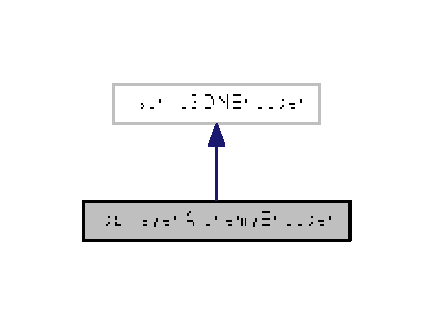
\includegraphics[width=208pt]{classdb__layer_1_1_alchemy_encoder__inherit__graph}
\end{center}
\end{figure}


Diagrama de colaboración para db\-\_\-layer.\-Alchemy\-Encoder\-:\nopagebreak
\begin{figure}[H]
\begin{center}
\leavevmode
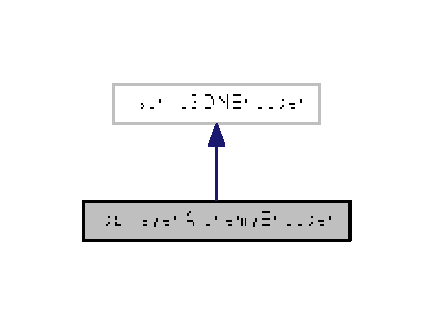
\includegraphics[width=208pt]{classdb__layer_1_1_alchemy_encoder__coll__graph}
\end{center}
\end{figure}
\subsection*{Métodos públicos}
\begin{DoxyCompactItemize}
\item 
def \hyperlink{classdb__layer_1_1_alchemy_encoder_abe41d36769d9edad84e480fed20c96f7}{default}
\end{DoxyCompactItemize}


\subsection{Descripción detallada}


Definición en la línea 80 del archivo db\-\_\-layer.\-py.



\subsection{Documentación de las funciones miembro}
\hypertarget{classdb__layer_1_1_alchemy_encoder_abe41d36769d9edad84e480fed20c96f7}{\index{db\-\_\-layer\-::\-Alchemy\-Encoder@{db\-\_\-layer\-::\-Alchemy\-Encoder}!default@{default}}
\index{default@{default}!db_layer::AlchemyEncoder@{db\-\_\-layer\-::\-Alchemy\-Encoder}}
\subsubsection[{default}]{\setlength{\rightskip}{0pt plus 5cm}def db\-\_\-layer.\-Alchemy\-Encoder.\-default (
\begin{DoxyParamCaption}
\item[{}]{self, }
\item[{}]{obj}
\end{DoxyParamCaption}
)}}\label{classdb__layer_1_1_alchemy_encoder_abe41d36769d9edad84e480fed20c96f7}


Definición en la línea 81 del archivo db\-\_\-layer.\-py.



La documentación para esta clase fue generada a partir del siguiente fichero\-:\begin{DoxyCompactItemize}
\item 
\hyperlink{db__layer_8py}{db\-\_\-layer.\-py}\end{DoxyCompactItemize}

\hypertarget{class_headers_1_1_client_headers}{\section{Referencia de la Clase Headers.\-Client\-Headers}
\label{class_headers_1_1_client_headers}\index{Headers.\-Client\-Headers@{Headers.\-Client\-Headers}}
}


Diagrama de colaboración para Headers.\-Client\-Headers\-:\nopagebreak
\begin{figure}[H]
\begin{center}
\leavevmode
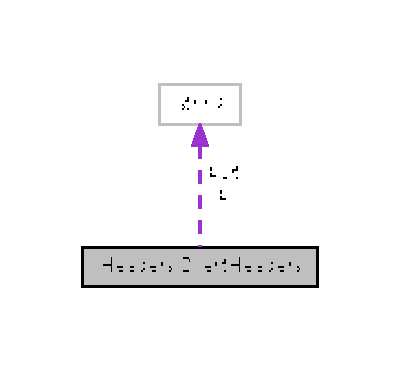
\includegraphics[width=192pt]{class_headers_1_1_client_headers__coll__graph}
\end{center}
\end{figure}
\subsection*{Métodos públicos}
\begin{DoxyCompactItemize}
\item 
def \hyperlink{class_headers_1_1_client_headers_a7dfc5b4ba33e104c0c4c320273583f06}{\-\_\-\-\_\-init\-\_\-\-\_\-}
\item 
def \hyperlink{class_headers_1_1_client_headers_a7ee0d7e2c47c1c9810e8427116479f3d}{parse}
\end{DoxyCompactItemize}
\subsection*{Atributos públicos}
\begin{DoxyCompactItemize}
\item 
\hyperlink{class_headers_1_1_client_headers_ad6a52ab3ffc9bdb7a023e8b42ce7083a}{D\-E\-B\-U\-G}
\item 
\hyperlink{class_headers_1_1_client_headers_a3b830916eb5f486466733a631debd80f}{ip}
\item 
\hyperlink{class_headers_1_1_client_headers_af5c53154eabf8999c0445d47c2ec2e93}{port}
\end{DoxyCompactItemize}
\subsection*{Atributos públicos estáticos}
\begin{DoxyCompactItemize}
\item 
list \hyperlink{class_headers_1_1_client_headers_a94f0846ec0ba5288c82e0cc43f240f78}{D\-E\-B\-U\-G} = Config.\-D\-E\-B\-U\-G\mbox{[}'Client\-Headers.\-D\-E\-B\-U\-G'\mbox{]}
\item 
string \hyperlink{class_headers_1_1_client_headers_a15b94d4c64d520378cf021770469ff74}{ip} = ''
\item 
string \hyperlink{class_headers_1_1_client_headers_a6f9c18e89358e04c9c869aec27095d74}{port} = ''
\item 
tuple \hyperlink{class_headers_1_1_client_headers_a5502fdd869b7ab7185c1049cbe5a534c}{log} = \hyperlink{class_log_1_1_log}{Log}()
\end{DoxyCompactItemize}


\subsection{Descripción detallada}


Definición en la línea 9 del archivo Headers.\-py.



\subsection{Documentación del constructor y destructor}
\hypertarget{class_headers_1_1_client_headers_a7dfc5b4ba33e104c0c4c320273583f06}{\index{Headers\-::\-Client\-Headers@{Headers\-::\-Client\-Headers}!\-\_\-\-\_\-init\-\_\-\-\_\-@{\-\_\-\-\_\-init\-\_\-\-\_\-}}
\index{\-\_\-\-\_\-init\-\_\-\-\_\-@{\-\_\-\-\_\-init\-\_\-\-\_\-}!Headers::ClientHeaders@{Headers\-::\-Client\-Headers}}
\subsubsection[{\-\_\-\-\_\-init\-\_\-\-\_\-}]{\setlength{\rightskip}{0pt plus 5cm}def Headers.\-Client\-Headers.\-\_\-\-\_\-init\-\_\-\-\_\- (
\begin{DoxyParamCaption}
\item[{}]{self, }
\item[{}]{headers, }
\item[{}]{debug = {\ttfamily False}, }
\item[{}]{ip = {\ttfamily ''}, }
\item[{}]{port = {\ttfamily ''}}
\end{DoxyParamCaption}
)}}\label{class_headers_1_1_client_headers_a7dfc5b4ba33e104c0c4c320273583f06}


Definición en la línea 19 del archivo Headers.\-py.



\subsection{Documentación de las funciones miembro}
\hypertarget{class_headers_1_1_client_headers_a7ee0d7e2c47c1c9810e8427116479f3d}{\index{Headers\-::\-Client\-Headers@{Headers\-::\-Client\-Headers}!parse@{parse}}
\index{parse@{parse}!Headers::ClientHeaders@{Headers\-::\-Client\-Headers}}
\subsubsection[{parse}]{\setlength{\rightskip}{0pt plus 5cm}def Headers.\-Client\-Headers.\-parse (
\begin{DoxyParamCaption}
\item[{}]{self}
\end{DoxyParamCaption}
)}}\label{class_headers_1_1_client_headers_a7ee0d7e2c47c1c9810e8427116479f3d}


Definición en la línea 31 del archivo Headers.\-py.



\subsection{Documentación de los datos miembro}
\hypertarget{class_headers_1_1_client_headers_a94f0846ec0ba5288c82e0cc43f240f78}{\index{Headers\-::\-Client\-Headers@{Headers\-::\-Client\-Headers}!D\-E\-B\-U\-G@{D\-E\-B\-U\-G}}
\index{D\-E\-B\-U\-G@{D\-E\-B\-U\-G}!Headers::ClientHeaders@{Headers\-::\-Client\-Headers}}
\subsubsection[{D\-E\-B\-U\-G}]{\setlength{\rightskip}{0pt plus 5cm}list Headers.\-Client\-Headers.\-D\-E\-B\-U\-G = Config.\-D\-E\-B\-U\-G\mbox{[}'Client\-Headers.\-D\-E\-B\-U\-G'\mbox{]}\hspace{0.3cm}{\ttfamily [static]}}}\label{class_headers_1_1_client_headers_a94f0846ec0ba5288c82e0cc43f240f78}


Definición en la línea 10 del archivo Headers.\-py.

\hypertarget{class_headers_1_1_client_headers_ad6a52ab3ffc9bdb7a023e8b42ce7083a}{\index{Headers\-::\-Client\-Headers@{Headers\-::\-Client\-Headers}!D\-E\-B\-U\-G@{D\-E\-B\-U\-G}}
\index{D\-E\-B\-U\-G@{D\-E\-B\-U\-G}!Headers::ClientHeaders@{Headers\-::\-Client\-Headers}}
\subsubsection[{D\-E\-B\-U\-G}]{\setlength{\rightskip}{0pt plus 5cm}Headers.\-Client\-Headers.\-D\-E\-B\-U\-G}}\label{class_headers_1_1_client_headers_ad6a52ab3ffc9bdb7a023e8b42ce7083a}


Definición en la línea 23 del archivo Headers.\-py.

\hypertarget{class_headers_1_1_client_headers_a15b94d4c64d520378cf021770469ff74}{\index{Headers\-::\-Client\-Headers@{Headers\-::\-Client\-Headers}!ip@{ip}}
\index{ip@{ip}!Headers::ClientHeaders@{Headers\-::\-Client\-Headers}}
\subsubsection[{ip}]{\setlength{\rightskip}{0pt plus 5cm}string Headers.\-Client\-Headers.\-ip = ''\hspace{0.3cm}{\ttfamily [static]}}}\label{class_headers_1_1_client_headers_a15b94d4c64d520378cf021770469ff74}


Definición en la línea 14 del archivo Headers.\-py.

\hypertarget{class_headers_1_1_client_headers_a3b830916eb5f486466733a631debd80f}{\index{Headers\-::\-Client\-Headers@{Headers\-::\-Client\-Headers}!ip@{ip}}
\index{ip@{ip}!Headers::ClientHeaders@{Headers\-::\-Client\-Headers}}
\subsubsection[{ip}]{\setlength{\rightskip}{0pt plus 5cm}Headers.\-Client\-Headers.\-ip}}\label{class_headers_1_1_client_headers_a3b830916eb5f486466733a631debd80f}


Definición en la línea 24 del archivo Headers.\-py.

\hypertarget{class_headers_1_1_client_headers_a5502fdd869b7ab7185c1049cbe5a534c}{\index{Headers\-::\-Client\-Headers@{Headers\-::\-Client\-Headers}!log@{log}}
\index{log@{log}!Headers::ClientHeaders@{Headers\-::\-Client\-Headers}}
\subsubsection[{log}]{\setlength{\rightskip}{0pt plus 5cm}tuple Headers.\-Client\-Headers.\-log = {\bf Log}()\hspace{0.3cm}{\ttfamily [static]}}}\label{class_headers_1_1_client_headers_a5502fdd869b7ab7185c1049cbe5a534c}


Definición en la línea 16 del archivo Headers.\-py.

\hypertarget{class_headers_1_1_client_headers_a6f9c18e89358e04c9c869aec27095d74}{\index{Headers\-::\-Client\-Headers@{Headers\-::\-Client\-Headers}!port@{port}}
\index{port@{port}!Headers::ClientHeaders@{Headers\-::\-Client\-Headers}}
\subsubsection[{port}]{\setlength{\rightskip}{0pt plus 5cm}string Headers.\-Client\-Headers.\-port = ''\hspace{0.3cm}{\ttfamily [static]}}}\label{class_headers_1_1_client_headers_a6f9c18e89358e04c9c869aec27095d74}


Definición en la línea 15 del archivo Headers.\-py.

\hypertarget{class_headers_1_1_client_headers_af5c53154eabf8999c0445d47c2ec2e93}{\index{Headers\-::\-Client\-Headers@{Headers\-::\-Client\-Headers}!port@{port}}
\index{port@{port}!Headers::ClientHeaders@{Headers\-::\-Client\-Headers}}
\subsubsection[{port}]{\setlength{\rightskip}{0pt plus 5cm}Headers.\-Client\-Headers.\-port}}\label{class_headers_1_1_client_headers_af5c53154eabf8999c0445d47c2ec2e93}


Definición en la línea 25 del archivo Headers.\-py.



La documentación para esta clase fue generada a partir del siguiente fichero\-:\begin{DoxyCompactItemize}
\item 
\hyperlink{_headers_8py}{Headers.\-py}\end{DoxyCompactItemize}

\hypertarget{class_config_1_1_config}{\section{Referencia de la Clase Config.\-Config}
\label{class_config_1_1_config}\index{Config.\-Config@{Config.\-Config}}
}


Diagrama de colaboración para Config.\-Config\-:\nopagebreak
\begin{figure}[H]
\begin{center}
\leavevmode
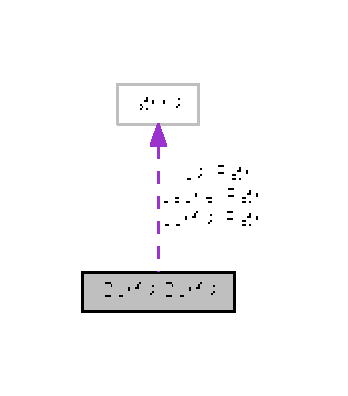
\includegraphics[width=167pt]{class_config_1_1_config__coll__graph}
\end{center}
\end{figure}
\subsection*{Atributos públicos estáticos}
\begin{DoxyCompactItemize}
\item 
int \hyperlink{class_config_1_1_config_a81b4f232892a63987c0712d291d68cd3}{M\-A\-X\-\_\-\-L\-E\-N\-\_\-\-M\-S\-G} = 140
\item 
int \hyperlink{class_config_1_1_config_a30a0b4f26a731f1f315b86b16eef807c}{N\-U\-M\-\_\-\-T\-H\-R\-E\-A\-D\-S} = 180
\item 
int \hyperlink{class_config_1_1_config_aef20c383d5c356bfc5771e132ad241df}{P\-O\-R\-T} = 8002
\item 
string \hyperlink{class_config_1_1_config_a2cf86b6dc19ce8b8458261d408a66d3a}{config\-\_\-\-Path} = \char`\"{}./db\char`\"{}
\item 
string \hyperlink{class_config_1_1_config_ac40dcb73f850406655e85747ee4f244a}{cache\-\_\-\-Path} = \char`\"{}./cache\char`\"{}
\item 
string \hyperlink{class_config_1_1_config_a101073e22bb0e11ae1e78063267eaf35}{log\-\_\-\-Path} = \char`\"{}./cache\char`\"{}
\item 
dictionary \hyperlink{class_config_1_1_config_a62ca676b07391529a5c1abd433bed57f}{db\-Files}
\item 
dictionary \hyperlink{class_config_1_1_config_af7a49b43885faa51f5f5b5687a05120c}{db\-Trace}
\item 
dictionary \hyperlink{class_config_1_1_config_a1d5bf72f9f7f8047bc648261155e3141}{D\-E\-B\-U\-G}
\item 
dictionary \hyperlink{class_config_1_1_config_aedf405e5fbfe131f86b5bde5de495fbc}{T\-R\-A\-C\-E}
\end{DoxyCompactItemize}


\subsection{Descripción detallada}


Definición en la línea 6 del archivo Config.\-py.



\subsection{Documentación de los datos miembro}
\hypertarget{class_config_1_1_config_ac40dcb73f850406655e85747ee4f244a}{\index{Config\-::\-Config@{Config\-::\-Config}!cache\-\_\-\-Path@{cache\-\_\-\-Path}}
\index{cache\-\_\-\-Path@{cache\-\_\-\-Path}!Config::Config@{Config\-::\-Config}}
\subsubsection[{cache\-\_\-\-Path}]{\setlength{\rightskip}{0pt plus 5cm}string Config.\-Config.\-cache\-\_\-\-Path = \char`\"{}./cache\char`\"{}\hspace{0.3cm}{\ttfamily [static]}}}\label{class_config_1_1_config_ac40dcb73f850406655e85747ee4f244a}


Definición en la línea 12 del archivo Config.\-py.

\hypertarget{class_config_1_1_config_a2cf86b6dc19ce8b8458261d408a66d3a}{\index{Config\-::\-Config@{Config\-::\-Config}!config\-\_\-\-Path@{config\-\_\-\-Path}}
\index{config\-\_\-\-Path@{config\-\_\-\-Path}!Config::Config@{Config\-::\-Config}}
\subsubsection[{config\-\_\-\-Path}]{\setlength{\rightskip}{0pt plus 5cm}string Config.\-Config.\-config\-\_\-\-Path = \char`\"{}./db\char`\"{}\hspace{0.3cm}{\ttfamily [static]}}}\label{class_config_1_1_config_a2cf86b6dc19ce8b8458261d408a66d3a}


Definición en la línea 11 del archivo Config.\-py.

\hypertarget{class_config_1_1_config_a62ca676b07391529a5c1abd433bed57f}{\index{Config\-::\-Config@{Config\-::\-Config}!db\-Files@{db\-Files}}
\index{db\-Files@{db\-Files}!Config::Config@{Config\-::\-Config}}
\subsubsection[{db\-Files}]{\setlength{\rightskip}{0pt plus 5cm}dictionary Config.\-Config.\-db\-Files\hspace{0.3cm}{\ttfamily [static]}}}\label{class_config_1_1_config_a62ca676b07391529a5c1abd433bed57f}
{\bfseries Valor inicial\-:}
\begin{DoxyCode}
1 = \{
2         \textcolor{stringliteral}{'proxy'}: \textcolor{stringliteral}{'sqlite:///'} + config\_Path+\textcolor{stringliteral}{'/proxy.db'},
3         \textcolor{stringliteral}{'log'}: \textcolor{stringliteral}{'sqlite:///'} + config\_Path+\textcolor{stringliteral}{'/log.db'}
4     \}
\end{DoxyCode}


Definición en la línea 15 del archivo Config.\-py.

\hypertarget{class_config_1_1_config_af7a49b43885faa51f5f5b5687a05120c}{\index{Config\-::\-Config@{Config\-::\-Config}!db\-Trace@{db\-Trace}}
\index{db\-Trace@{db\-Trace}!Config::Config@{Config\-::\-Config}}
\subsubsection[{db\-Trace}]{\setlength{\rightskip}{0pt plus 5cm}dictionary Config.\-Config.\-db\-Trace\hspace{0.3cm}{\ttfamily [static]}}}\label{class_config_1_1_config_af7a49b43885faa51f5f5b5687a05120c}
{\bfseries Valor inicial\-:}
\begin{DoxyCode}
1 = \{
2         \textcolor{stringliteral}{'proxy'}: \textcolor{keyword}{False},
3         \textcolor{stringliteral}{'log'}: \textcolor{keyword}{False}
4     \}
\end{DoxyCode}


Definición en la línea 20 del archivo Config.\-py.

\hypertarget{class_config_1_1_config_a1d5bf72f9f7f8047bc648261155e3141}{\index{Config\-::\-Config@{Config\-::\-Config}!D\-E\-B\-U\-G@{D\-E\-B\-U\-G}}
\index{D\-E\-B\-U\-G@{D\-E\-B\-U\-G}!Config::Config@{Config\-::\-Config}}
\subsubsection[{D\-E\-B\-U\-G}]{\setlength{\rightskip}{0pt plus 5cm}dictionary Config.\-Config.\-D\-E\-B\-U\-G\hspace{0.3cm}{\ttfamily [static]}}}\label{class_config_1_1_config_a1d5bf72f9f7f8047bc648261155e3141}
{\bfseries Valor inicial\-:}
\begin{DoxyCode}
1 = \{
2         \textcolor{stringliteral}{'db\_mapper.DEBUGCALL'} : \textcolor{keyword}{False},
3         \textcolor{stringliteral}{'db\_mapper.DEBUGANSWER'} : \textcolor{keyword}{False},
4         \textcolor{stringliteral}{'db\_mapper.DEBUG'} : \textcolor{keyword}{False},
5         \textcolor{stringliteral}{'Proxy.DEBUG'}: \textcolor{keyword}{False},
6         \textcolor{stringliteral}{'Proxy.DEBUG\_BEFORE\_HANDLING'}: \textcolor{keyword}{False},
7         \textcolor{stringliteral}{'Cache.DEBUG'}: \textcolor{keyword}{False},
8         \textcolor{stringliteral}{'ClientHeaders.DEBUG'}: \textcolor{keyword}{False},
9         \textcolor{stringliteral}{'ServerHeaders.DEBUG'}: \textcolor{keyword}{False},
10     \}
\end{DoxyCode}


Definición en la línea 25 del archivo Config.\-py.

\hypertarget{class_config_1_1_config_a101073e22bb0e11ae1e78063267eaf35}{\index{Config\-::\-Config@{Config\-::\-Config}!log\-\_\-\-Path@{log\-\_\-\-Path}}
\index{log\-\_\-\-Path@{log\-\_\-\-Path}!Config::Config@{Config\-::\-Config}}
\subsubsection[{log\-\_\-\-Path}]{\setlength{\rightskip}{0pt plus 5cm}string Config.\-Config.\-log\-\_\-\-Path = \char`\"{}./cache\char`\"{}\hspace{0.3cm}{\ttfamily [static]}}}\label{class_config_1_1_config_a101073e22bb0e11ae1e78063267eaf35}


Definición en la línea 13 del archivo Config.\-py.

\hypertarget{class_config_1_1_config_a81b4f232892a63987c0712d291d68cd3}{\index{Config\-::\-Config@{Config\-::\-Config}!M\-A\-X\-\_\-\-L\-E\-N\-\_\-\-M\-S\-G@{M\-A\-X\-\_\-\-L\-E\-N\-\_\-\-M\-S\-G}}
\index{M\-A\-X\-\_\-\-L\-E\-N\-\_\-\-M\-S\-G@{M\-A\-X\-\_\-\-L\-E\-N\-\_\-\-M\-S\-G}!Config::Config@{Config\-::\-Config}}
\subsubsection[{M\-A\-X\-\_\-\-L\-E\-N\-\_\-\-M\-S\-G}]{\setlength{\rightskip}{0pt plus 5cm}int Config.\-Config.\-M\-A\-X\-\_\-\-L\-E\-N\-\_\-\-M\-S\-G = 140\hspace{0.3cm}{\ttfamily [static]}}}\label{class_config_1_1_config_a81b4f232892a63987c0712d291d68cd3}


Definición en la línea 7 del archivo Config.\-py.

\hypertarget{class_config_1_1_config_a30a0b4f26a731f1f315b86b16eef807c}{\index{Config\-::\-Config@{Config\-::\-Config}!N\-U\-M\-\_\-\-T\-H\-R\-E\-A\-D\-S@{N\-U\-M\-\_\-\-T\-H\-R\-E\-A\-D\-S}}
\index{N\-U\-M\-\_\-\-T\-H\-R\-E\-A\-D\-S@{N\-U\-M\-\_\-\-T\-H\-R\-E\-A\-D\-S}!Config::Config@{Config\-::\-Config}}
\subsubsection[{N\-U\-M\-\_\-\-T\-H\-R\-E\-A\-D\-S}]{\setlength{\rightskip}{0pt plus 5cm}int Config.\-Config.\-N\-U\-M\-\_\-\-T\-H\-R\-E\-A\-D\-S = 180\hspace{0.3cm}{\ttfamily [static]}}}\label{class_config_1_1_config_a30a0b4f26a731f1f315b86b16eef807c}


Definición en la línea 8 del archivo Config.\-py.

\hypertarget{class_config_1_1_config_aef20c383d5c356bfc5771e132ad241df}{\index{Config\-::\-Config@{Config\-::\-Config}!P\-O\-R\-T@{P\-O\-R\-T}}
\index{P\-O\-R\-T@{P\-O\-R\-T}!Config::Config@{Config\-::\-Config}}
\subsubsection[{P\-O\-R\-T}]{\setlength{\rightskip}{0pt plus 5cm}int Config.\-Config.\-P\-O\-R\-T = 8002\hspace{0.3cm}{\ttfamily [static]}}}\label{class_config_1_1_config_aef20c383d5c356bfc5771e132ad241df}


Definición en la línea 9 del archivo Config.\-py.

\hypertarget{class_config_1_1_config_aedf405e5fbfe131f86b5bde5de495fbc}{\index{Config\-::\-Config@{Config\-::\-Config}!T\-R\-A\-C\-E@{T\-R\-A\-C\-E}}
\index{T\-R\-A\-C\-E@{T\-R\-A\-C\-E}!Config::Config@{Config\-::\-Config}}
\subsubsection[{T\-R\-A\-C\-E}]{\setlength{\rightskip}{0pt plus 5cm}dictionary Config.\-Config.\-T\-R\-A\-C\-E\hspace{0.3cm}{\ttfamily [static]}}}\label{class_config_1_1_config_aedf405e5fbfe131f86b5bde5de495fbc}
{\bfseries Valor inicial\-:}
\begin{DoxyCode}
1 = \{
2         \textcolor{stringliteral}{'Log\_TRACE'}: \textcolor{keyword}{True}
3     \}
\end{DoxyCode}


Definición en la línea 36 del archivo Config.\-py.



La documentación para esta clase fue generada a partir del siguiente fichero\-:\begin{DoxyCompactItemize}
\item 
\hyperlink{_config_8py}{Config.\-py}\end{DoxyCompactItemize}

\hypertarget{classdb__layer_1_1_database}{\section{Referencia de la Clase db\-\_\-layer.\-Database}
\label{classdb__layer_1_1_database}\index{db\-\_\-layer.\-Database@{db\-\_\-layer.\-Database}}
}
\subsection*{Métodos públicos}
\begin{DoxyCompactItemize}
\item 
def \hyperlink{classdb__layer_1_1_database_a2e4b8be9ebcb91f37e9377164e060c2a}{\-\_\-\-\_\-init\-\_\-\-\_\-}
\item 
def \hyperlink{classdb__layer_1_1_database_aaa54107650dc6511c7afdaf98112d4c1}{find\-User}
\item 
def \hyperlink{classdb__layer_1_1_database_a321ec63103a76c21fb556f82bc03e08f}{find\-User\-By\-Username}
\item 
def \hyperlink{classdb__layer_1_1_database_a738e07ff3b7292931bb057d174866249}{is\-User\-Allowed}
\item 
def \hyperlink{classdb__layer_1_1_database_a1f4a9b4e8dbd15d9f0ce74c1464ec3f9}{is\-Admin\-Allowed}
\item 
def \hyperlink{classdb__layer_1_1_database_aa97a7c93c41d97e60600dec9fb87270e}{find\-User\-By\-U\-I\-D}
\item 
def \hyperlink{classdb__layer_1_1_database_aa56ec835e0baf06452952528e12062bc}{get\-All\-User}
\item 
def \hyperlink{classdb__layer_1_1_database_a99ba044bb2e8692e27c34b74f6420ce8}{get\-Lowest\-Unused\-U\-I\-Dfrom\-User}
\item 
def \hyperlink{classdb__layer_1_1_database_a607d0253401fe69017f3e2b397a66c65}{add\-User}
\item 
def \hyperlink{classdb__layer_1_1_database_a1d5f62d1f3ee91d692483abe8c774c89}{add\-Relation}
\item 
def \hyperlink{classdb__layer_1_1_database_aa682552b52caba32fde23ef44fb63ade}{wr\-\_\-add\-Relation}
\item 
def \hyperlink{classdb__layer_1_1_database_ab4e221a9ae93a5780c084d49d01029d8}{del\-Relation}
\item 
def \hyperlink{classdb__layer_1_1_database_ab20da0ac6137c6a276f27f59a90d87e3}{wr\-\_\-del\-Relation}
\item 
def \hyperlink{classdb__layer_1_1_database_ad8447f580fdb6dc37c23fe4220ee62b9}{del\-User}
\item 
def \hyperlink{classdb__layer_1_1_database_a03795c597d3a3ca0ef5d7c73299f8421}{set\-User\-Admin}
\item 
def \hyperlink{classdb__layer_1_1_database_a6b55a92453cf88fd95b0e6b565663bbc}{change\-User}
\item 
def \hyperlink{classdb__layer_1_1_database_a203864bb4a53dfb89f57c23392559b46}{set\-User\-Advanced}
\item 
def \hyperlink{classdb__layer_1_1_database_a03a583931163ed9bac45c5b05e4bf69f}{set\-User\-Kid}
\item 
def \hyperlink{classdb__layer_1_1_database_ab86b18a8ab851b48703101ab53af6f8b}{set\-User\-Guest}
\item 
def \hyperlink{classdb__layer_1_1_database_a2faddc3de17c5f91a96d835339e5b187}{change\-User\-Password}
\item 
def \hyperlink{classdb__layer_1_1_database_ad49eca83ffa1263e355f5757e9b4d814}{change\-User\-Description}
\item 
def \hyperlink{classdb__layer_1_1_database_a3cdf214f598de4b4c5d08e5a1f7c218b}{commit\-D\-B\-Changes}
\item 
def \hyperlink{classdb__layer_1_1_database_a39d62bdcc06c57e3a02aa86c31a45f8d}{find\-Group}
\item 
def \hyperlink{classdb__layer_1_1_database_a20c7dd43617755b5ebaf0e1d22a4a2f8}{find\-Group\-By\-Groupname}
\item 
def \hyperlink{classdb__layer_1_1_database_a16008b08c96fa493d7ee12b2a7a5b181}{find\-Group\-By\-G\-I\-D}
\item 
def \hyperlink{classdb__layer_1_1_database_a8470bd9042a562ac6205dc6edcb374ea}{del\-Group}
\item 
def \hyperlink{classdb__layer_1_1_database_a36251bcd67a2b86157830f7c4df7c35d}{change\-Group}
\item 
def \hyperlink{classdb__layer_1_1_database_aec26922467f83a27ddc41b583f0f1cb0}{get\-All\-Groups}
\item 
def \hyperlink{classdb__layer_1_1_database_a22ed5c7f36dbb61e6f60c4040987bf55}{get\-All\-Custom\-Groups}
\item 
def \hyperlink{classdb__layer_1_1_database_a98fa2d3a8377bca1fe5f2d2946ef2929}{get\-Lowest\-Unused\-G\-I\-Dfrom\-Group}
\item 
def \hyperlink{classdb__layer_1_1_database_a472b95b106b4fe0185582d99f36edb85}{add\-Group}
\item 
def \hyperlink{classdb__layer_1_1_database_ab3e162f3cda68dacdfaa3de68e300567}{change\-Group\-Description}
\item 
def \hyperlink{classdb__layer_1_1_database_af6ba4fcf6bcd589b0c85b05f49f46ef5}{is\-User\-Allowed\-Now}
\item 
def \hyperlink{classdb__layer_1_1_database_a9ddac6b8ec475ecd6e817329416e3d22}{is\-User\-Admin}
\item 
def \hyperlink{classdb__layer_1_1_database_abbe6297269170e88f0ebe7da784fb62b}{is\-User\-Advanced}
\item 
def \hyperlink{classdb__layer_1_1_database_a3aaf3d095b7c6d005ec9061f83ccdc66}{is\-User\-Kid}
\item 
def \hyperlink{classdb__layer_1_1_database_a9ff75e8e93503e1e6b5ceb083910864a}{is\-User\-Guest}
\item 
def \hyperlink{classdb__layer_1_1_database_acf2271857a561c1e17069068f5c7e317}{find\-Groups\-By\-User}
\item 
def \hyperlink{classdb__layer_1_1_database_a782bfdf0a4415ef9f520722125851924}{find\-Not\-Groups\-By\-User}
\item 
def \hyperlink{classdb__layer_1_1_database_abe7e2fc7937e3fd641a8ec5275b4db60}{find\-U\-R\-I\-Sby\-G\-I\-D}
\item 
def \hyperlink{classdb__layer_1_1_database_a9182f4e89992da5de14ae67f466514df}{delete\-U\-R\-I\-Sby\-G\-I\-D}
\item 
def \hyperlink{classdb__layer_1_1_database_aebc7fd132c862539ede9959fa4257d2a}{insert\-U\-R\-I\-Sby\-G\-I\-D}
\item 
def \hyperlink{classdb__layer_1_1_database_a3ede692ddfa18fd73ce142341f21e6a0}{wr\-\_\-insert\-U\-R\-I\-Sby\-G\-I\-D}
\item 
def \hyperlink{classdb__layer_1_1_database_a7f168024109c6490cca9f764cd0bbeac}{find\-W\-O\-R\-D\-Sby\-G\-I\-D}
\item 
def \hyperlink{classdb__layer_1_1_database_af7c91fdd73898b9e2aa1d1e04ebcb8a6}{delete\-W\-O\-R\-D\-Sby\-G\-I\-D}
\item 
def \hyperlink{classdb__layer_1_1_database_a849faf2993ee0d75f38639f22c3553e7}{insert\-W\-O\-R\-D\-Sby\-G\-I\-D}
\item 
def \hyperlink{classdb__layer_1_1_database_abf6ce37aea5202f161dbd3e3c41d6a6e}{wr\-\_\-insert\-W\-O\-R\-D\-Sby\-G\-I\-D}
\item 
def \hyperlink{classdb__layer_1_1_database_a940f5d9df2aa98c4c4452d9a005a0788}{find\-M\-I\-M\-E\-Sby\-G\-I\-D}
\item 
def \hyperlink{classdb__layer_1_1_database_a844ac1872f0ddf55d238e2bc229354c0}{delete\-M\-I\-M\-E\-Sby\-G\-I\-D}
\item 
def \hyperlink{classdb__layer_1_1_database_ae95955bc5ae21324a753dca4d76f69f1}{insert\-M\-I\-M\-E\-Sby\-G\-I\-D}
\item 
def \hyperlink{classdb__layer_1_1_database_ac2a8936466701acf8972dd1dbb73d0ad}{wr\-\_\-insert\-M\-I\-M\-E\-Sby\-G\-I\-D}
\item 
def \hyperlink{classdb__layer_1_1_database_a014383f7f432ef974c12c87bdbe08546}{get\-R\-U\-L\-E\-S}
\end{DoxyCompactItemize}
\subsection*{Atributos públicos estáticos}
\begin{DoxyCompactItemize}
\item 
\hyperlink{classdb__layer_1_1_database_a232d5477efc9b4c8d8a36b7541c851e1}{session} = None
\end{DoxyCompactItemize}


\subsection{Descripción detallada}


Definición en la línea 104 del archivo db\-\_\-layer.\-py.



\subsection{Documentación del constructor y destructor}
\hypertarget{classdb__layer_1_1_database_a2e4b8be9ebcb91f37e9377164e060c2a}{\index{db\-\_\-layer\-::\-Database@{db\-\_\-layer\-::\-Database}!\-\_\-\-\_\-init\-\_\-\-\_\-@{\-\_\-\-\_\-init\-\_\-\-\_\-}}
\index{\-\_\-\-\_\-init\-\_\-\-\_\-@{\-\_\-\-\_\-init\-\_\-\-\_\-}!db_layer::Database@{db\-\_\-layer\-::\-Database}}
\subsubsection[{\-\_\-\-\_\-init\-\_\-\-\_\-}]{\setlength{\rightskip}{0pt plus 5cm}def db\-\_\-layer.\-Database.\-\_\-\-\_\-init\-\_\-\-\_\- (
\begin{DoxyParamCaption}
\item[{}]{self}
\end{DoxyParamCaption}
)}}\label{classdb__layer_1_1_database_a2e4b8be9ebcb91f37e9377164e060c2a}


Definición en la línea 110 del archivo db\-\_\-layer.\-py.



\subsection{Documentación de las funciones miembro}
\hypertarget{classdb__layer_1_1_database_a472b95b106b4fe0185582d99f36edb85}{\index{db\-\_\-layer\-::\-Database@{db\-\_\-layer\-::\-Database}!add\-Group@{add\-Group}}
\index{add\-Group@{add\-Group}!db_layer::Database@{db\-\_\-layer\-::\-Database}}
\subsubsection[{add\-Group}]{\setlength{\rightskip}{0pt plus 5cm}def db\-\_\-layer.\-Database.\-add\-Group (
\begin{DoxyParamCaption}
\item[{}]{self, }
\item[{}]{new\-Group}
\end{DoxyParamCaption}
)}}\label{classdb__layer_1_1_database_a472b95b106b4fe0185582d99f36edb85}


Definición en la línea 560 del archivo db\-\_\-layer.\-py.



Gráfico de llamadas para esta función\-:\nopagebreak
\begin{figure}[H]
\begin{center}
\leavevmode
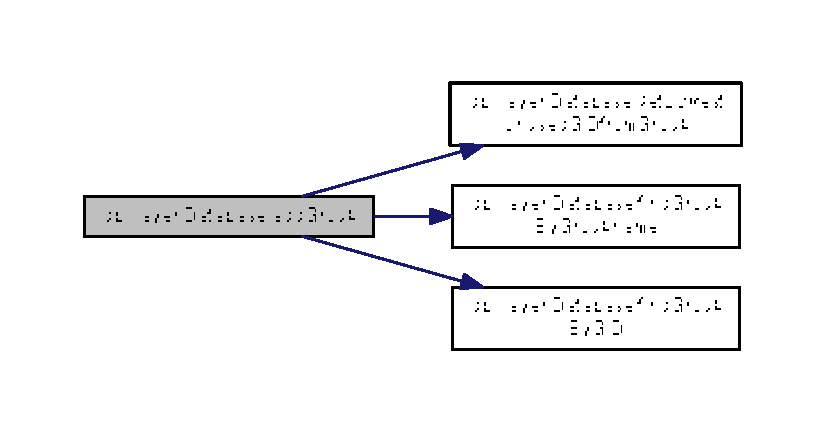
\includegraphics[width=350pt]{classdb__layer_1_1_database_a472b95b106b4fe0185582d99f36edb85_cgraph}
\end{center}
\end{figure}


\hypertarget{classdb__layer_1_1_database_a1d5f62d1f3ee91d692483abe8c774c89}{\index{db\-\_\-layer\-::\-Database@{db\-\_\-layer\-::\-Database}!add\-Relation@{add\-Relation}}
\index{add\-Relation@{add\-Relation}!db_layer::Database@{db\-\_\-layer\-::\-Database}}
\subsubsection[{add\-Relation}]{\setlength{\rightskip}{0pt plus 5cm}def db\-\_\-layer.\-Database.\-add\-Relation (
\begin{DoxyParamCaption}
\item[{}]{self, }
\item[{}]{uid, }
\item[{}]{gid}
\end{DoxyParamCaption}
)}}\label{classdb__layer_1_1_database_a1d5f62d1f3ee91d692483abe8c774c89}


Definición en la línea 269 del archivo db\-\_\-layer.\-py.



Gráfico de llamadas para esta función\-:\nopagebreak
\begin{figure}[H]
\begin{center}
\leavevmode
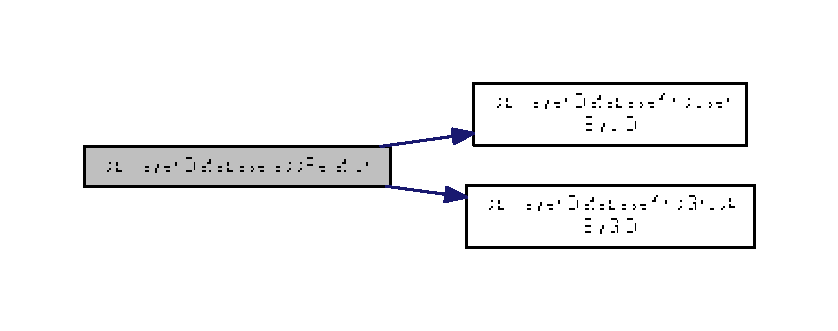
\includegraphics[width=350pt]{classdb__layer_1_1_database_a1d5f62d1f3ee91d692483abe8c774c89_cgraph}
\end{center}
\end{figure}




Gráfico de llamadas a esta función\-:\nopagebreak
\begin{figure}[H]
\begin{center}
\leavevmode
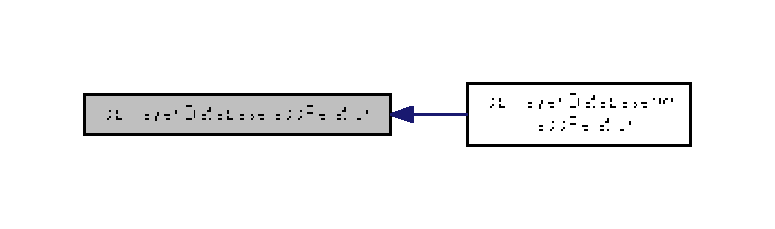
\includegraphics[width=350pt]{classdb__layer_1_1_database_a1d5f62d1f3ee91d692483abe8c774c89_icgraph}
\end{center}
\end{figure}


\hypertarget{classdb__layer_1_1_database_a607d0253401fe69017f3e2b397a66c65}{\index{db\-\_\-layer\-::\-Database@{db\-\_\-layer\-::\-Database}!add\-User@{add\-User}}
\index{add\-User@{add\-User}!db_layer::Database@{db\-\_\-layer\-::\-Database}}
\subsubsection[{add\-User}]{\setlength{\rightskip}{0pt plus 5cm}def db\-\_\-layer.\-Database.\-add\-User (
\begin{DoxyParamCaption}
\item[{}]{self, }
\item[{}]{new\-User}
\end{DoxyParamCaption}
)}}\label{classdb__layer_1_1_database_a607d0253401fe69017f3e2b397a66c65}


Definición en la línea 206 del archivo db\-\_\-layer.\-py.



Gráfico de llamadas para esta función\-:\nopagebreak
\begin{figure}[H]
\begin{center}
\leavevmode
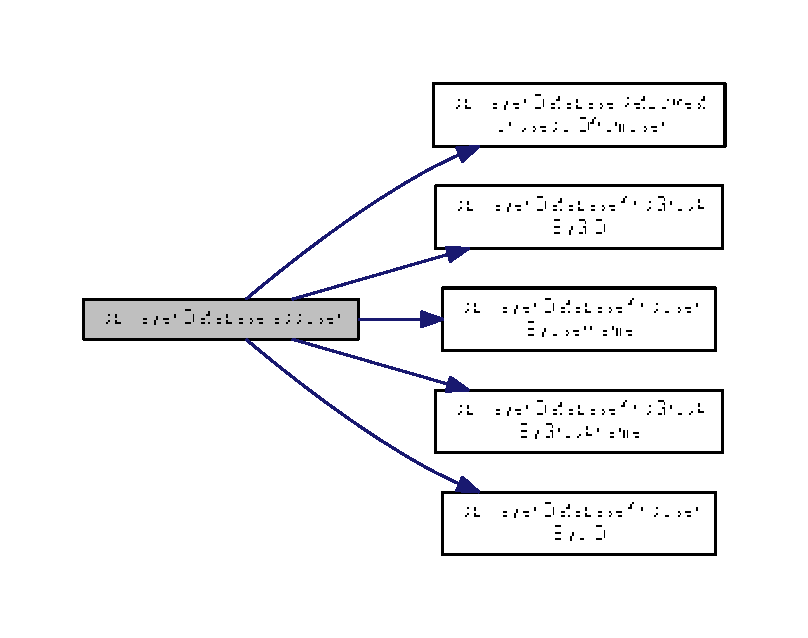
\includegraphics[width=350pt]{classdb__layer_1_1_database_a607d0253401fe69017f3e2b397a66c65_cgraph}
\end{center}
\end{figure}


\hypertarget{classdb__layer_1_1_database_a36251bcd67a2b86157830f7c4df7c35d}{\index{db\-\_\-layer\-::\-Database@{db\-\_\-layer\-::\-Database}!change\-Group@{change\-Group}}
\index{change\-Group@{change\-Group}!db_layer::Database@{db\-\_\-layer\-::\-Database}}
\subsubsection[{change\-Group}]{\setlength{\rightskip}{0pt plus 5cm}def db\-\_\-layer.\-Database.\-change\-Group (
\begin{DoxyParamCaption}
\item[{}]{self, }
\item[{}]{requested\-Group}
\end{DoxyParamCaption}
)}}\label{classdb__layer_1_1_database_a36251bcd67a2b86157830f7c4df7c35d}


Definición en la línea 519 del archivo db\-\_\-layer.\-py.



Gráfico de llamadas para esta función\-:\nopagebreak
\begin{figure}[H]
\begin{center}
\leavevmode
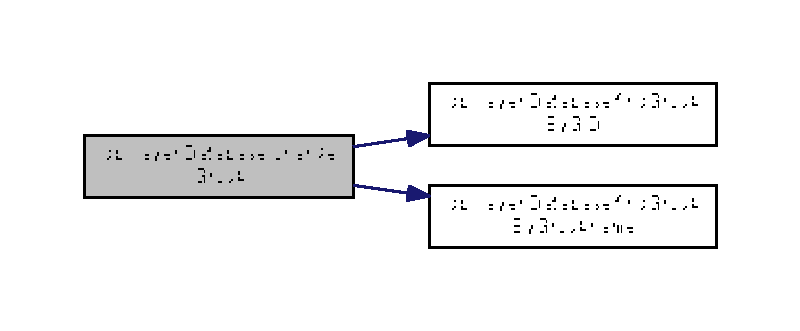
\includegraphics[width=350pt]{classdb__layer_1_1_database_a36251bcd67a2b86157830f7c4df7c35d_cgraph}
\end{center}
\end{figure}


\hypertarget{classdb__layer_1_1_database_ab3e162f3cda68dacdfaa3de68e300567}{\index{db\-\_\-layer\-::\-Database@{db\-\_\-layer\-::\-Database}!change\-Group\-Description@{change\-Group\-Description}}
\index{change\-Group\-Description@{change\-Group\-Description}!db_layer::Database@{db\-\_\-layer\-::\-Database}}
\subsubsection[{change\-Group\-Description}]{\setlength{\rightskip}{0pt plus 5cm}def db\-\_\-layer.\-Database.\-change\-Group\-Description (
\begin{DoxyParamCaption}
\item[{}]{self, }
\item[{}]{requested\-Group}
\end{DoxyParamCaption}
)}}\label{classdb__layer_1_1_database_ab3e162f3cda68dacdfaa3de68e300567}


Definición en la línea 591 del archivo db\-\_\-layer.\-py.



Gráfico de llamadas para esta función\-:\nopagebreak
\begin{figure}[H]
\begin{center}
\leavevmode
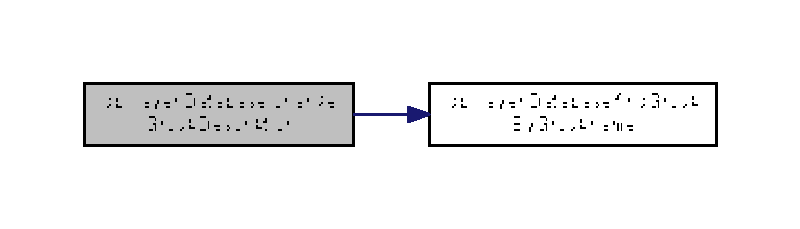
\includegraphics[width=350pt]{classdb__layer_1_1_database_ab3e162f3cda68dacdfaa3de68e300567_cgraph}
\end{center}
\end{figure}


\hypertarget{classdb__layer_1_1_database_a6b55a92453cf88fd95b0e6b565663bbc}{\index{db\-\_\-layer\-::\-Database@{db\-\_\-layer\-::\-Database}!change\-User@{change\-User}}
\index{change\-User@{change\-User}!db_layer::Database@{db\-\_\-layer\-::\-Database}}
\subsubsection[{change\-User}]{\setlength{\rightskip}{0pt plus 5cm}def db\-\_\-layer.\-Database.\-change\-User (
\begin{DoxyParamCaption}
\item[{}]{self, }
\item[{}]{requested\-User}
\end{DoxyParamCaption}
)}}\label{classdb__layer_1_1_database_a6b55a92453cf88fd95b0e6b565663bbc}


Definición en la línea 348 del archivo db\-\_\-layer.\-py.



Gráfico de llamadas para esta función\-:\nopagebreak
\begin{figure}[H]
\begin{center}
\leavevmode
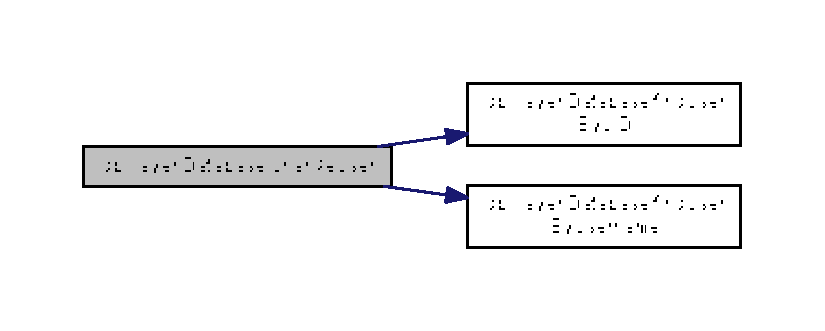
\includegraphics[width=350pt]{classdb__layer_1_1_database_a6b55a92453cf88fd95b0e6b565663bbc_cgraph}
\end{center}
\end{figure}


\hypertarget{classdb__layer_1_1_database_ad49eca83ffa1263e355f5757e9b4d814}{\index{db\-\_\-layer\-::\-Database@{db\-\_\-layer\-::\-Database}!change\-User\-Description@{change\-User\-Description}}
\index{change\-User\-Description@{change\-User\-Description}!db_layer::Database@{db\-\_\-layer\-::\-Database}}
\subsubsection[{change\-User\-Description}]{\setlength{\rightskip}{0pt plus 5cm}def db\-\_\-layer.\-Database.\-change\-User\-Description (
\begin{DoxyParamCaption}
\item[{}]{self, }
\item[{}]{requested\-User}
\end{DoxyParamCaption}
)}}\label{classdb__layer_1_1_database_ad49eca83ffa1263e355f5757e9b4d814}


Definición en la línea 438 del archivo db\-\_\-layer.\-py.



Gráfico de llamadas para esta función\-:\nopagebreak
\begin{figure}[H]
\begin{center}
\leavevmode
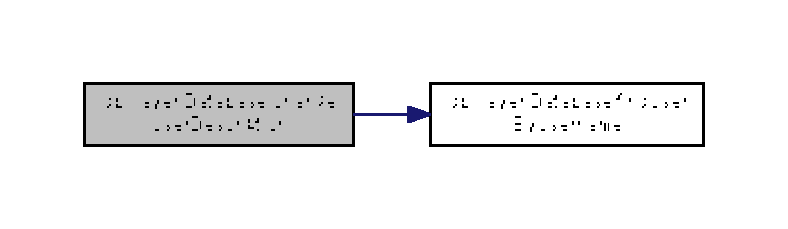
\includegraphics[width=350pt]{classdb__layer_1_1_database_ad49eca83ffa1263e355f5757e9b4d814_cgraph}
\end{center}
\end{figure}


\hypertarget{classdb__layer_1_1_database_a2faddc3de17c5f91a96d835339e5b187}{\index{db\-\_\-layer\-::\-Database@{db\-\_\-layer\-::\-Database}!change\-User\-Password@{change\-User\-Password}}
\index{change\-User\-Password@{change\-User\-Password}!db_layer::Database@{db\-\_\-layer\-::\-Database}}
\subsubsection[{change\-User\-Password}]{\setlength{\rightskip}{0pt plus 5cm}def db\-\_\-layer.\-Database.\-change\-User\-Password (
\begin{DoxyParamCaption}
\item[{}]{self, }
\item[{}]{requested\-User}
\end{DoxyParamCaption}
)}}\label{classdb__layer_1_1_database_a2faddc3de17c5f91a96d835339e5b187}


Definición en la línea 423 del archivo db\-\_\-layer.\-py.



Gráfico de llamadas para esta función\-:\nopagebreak
\begin{figure}[H]
\begin{center}
\leavevmode
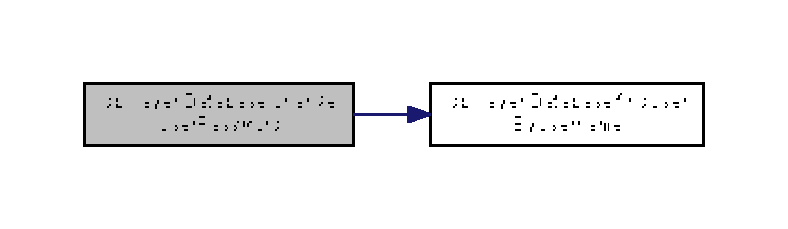
\includegraphics[width=350pt]{classdb__layer_1_1_database_a2faddc3de17c5f91a96d835339e5b187_cgraph}
\end{center}
\end{figure}


\hypertarget{classdb__layer_1_1_database_a3cdf214f598de4b4c5d08e5a1f7c218b}{\index{db\-\_\-layer\-::\-Database@{db\-\_\-layer\-::\-Database}!commit\-D\-B\-Changes@{commit\-D\-B\-Changes}}
\index{commit\-D\-B\-Changes@{commit\-D\-B\-Changes}!db_layer::Database@{db\-\_\-layer\-::\-Database}}
\subsubsection[{commit\-D\-B\-Changes}]{\setlength{\rightskip}{0pt plus 5cm}def db\-\_\-layer.\-Database.\-commit\-D\-B\-Changes (
\begin{DoxyParamCaption}
\item[{}]{self}
\end{DoxyParamCaption}
)}}\label{classdb__layer_1_1_database_a3cdf214f598de4b4c5d08e5a1f7c218b}


Definición en la línea 453 del archivo db\-\_\-layer.\-py.

\hypertarget{classdb__layer_1_1_database_a844ac1872f0ddf55d238e2bc229354c0}{\index{db\-\_\-layer\-::\-Database@{db\-\_\-layer\-::\-Database}!delete\-M\-I\-M\-E\-Sby\-G\-I\-D@{delete\-M\-I\-M\-E\-Sby\-G\-I\-D}}
\index{delete\-M\-I\-M\-E\-Sby\-G\-I\-D@{delete\-M\-I\-M\-E\-Sby\-G\-I\-D}!db_layer::Database@{db\-\_\-layer\-::\-Database}}
\subsubsection[{delete\-M\-I\-M\-E\-Sby\-G\-I\-D}]{\setlength{\rightskip}{0pt plus 5cm}def db\-\_\-layer.\-Database.\-delete\-M\-I\-M\-E\-Sby\-G\-I\-D (
\begin{DoxyParamCaption}
\item[{}]{self, }
\item[{}]{gid}
\end{DoxyParamCaption}
)}}\label{classdb__layer_1_1_database_a844ac1872f0ddf55d238e2bc229354c0}


Definición en la línea 854 del archivo db\-\_\-layer.\-py.



Gráfico de llamadas a esta función\-:\nopagebreak
\begin{figure}[H]
\begin{center}
\leavevmode
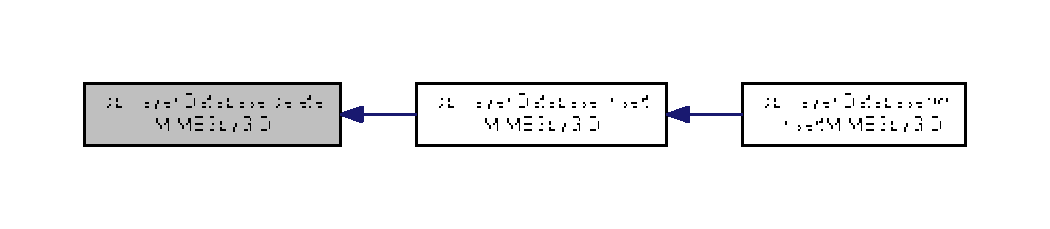
\includegraphics[width=350pt]{classdb__layer_1_1_database_a844ac1872f0ddf55d238e2bc229354c0_icgraph}
\end{center}
\end{figure}


\hypertarget{classdb__layer_1_1_database_a9182f4e89992da5de14ae67f466514df}{\index{db\-\_\-layer\-::\-Database@{db\-\_\-layer\-::\-Database}!delete\-U\-R\-I\-Sby\-G\-I\-D@{delete\-U\-R\-I\-Sby\-G\-I\-D}}
\index{delete\-U\-R\-I\-Sby\-G\-I\-D@{delete\-U\-R\-I\-Sby\-G\-I\-D}!db_layer::Database@{db\-\_\-layer\-::\-Database}}
\subsubsection[{delete\-U\-R\-I\-Sby\-G\-I\-D}]{\setlength{\rightskip}{0pt plus 5cm}def db\-\_\-layer.\-Database.\-delete\-U\-R\-I\-Sby\-G\-I\-D (
\begin{DoxyParamCaption}
\item[{}]{self, }
\item[{}]{gid}
\end{DoxyParamCaption}
)}}\label{classdb__layer_1_1_database_a9182f4e89992da5de14ae67f466514df}


Definición en la línea 759 del archivo db\-\_\-layer.\-py.



Gráfico de llamadas a esta función\-:\nopagebreak
\begin{figure}[H]
\begin{center}
\leavevmode
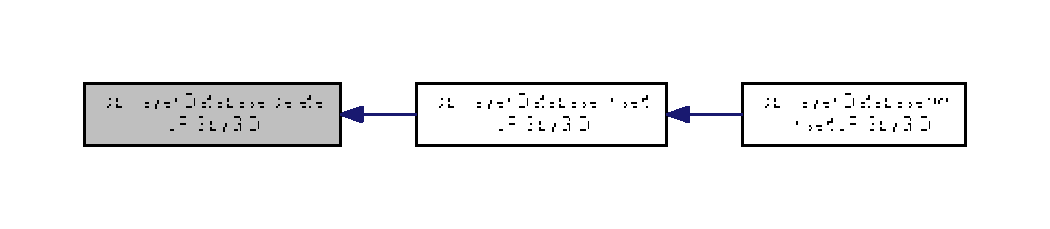
\includegraphics[width=350pt]{classdb__layer_1_1_database_a9182f4e89992da5de14ae67f466514df_icgraph}
\end{center}
\end{figure}


\hypertarget{classdb__layer_1_1_database_af7c91fdd73898b9e2aa1d1e04ebcb8a6}{\index{db\-\_\-layer\-::\-Database@{db\-\_\-layer\-::\-Database}!delete\-W\-O\-R\-D\-Sby\-G\-I\-D@{delete\-W\-O\-R\-D\-Sby\-G\-I\-D}}
\index{delete\-W\-O\-R\-D\-Sby\-G\-I\-D@{delete\-W\-O\-R\-D\-Sby\-G\-I\-D}!db_layer::Database@{db\-\_\-layer\-::\-Database}}
\subsubsection[{delete\-W\-O\-R\-D\-Sby\-G\-I\-D}]{\setlength{\rightskip}{0pt plus 5cm}def db\-\_\-layer.\-Database.\-delete\-W\-O\-R\-D\-Sby\-G\-I\-D (
\begin{DoxyParamCaption}
\item[{}]{self, }
\item[{}]{gid}
\end{DoxyParamCaption}
)}}\label{classdb__layer_1_1_database_af7c91fdd73898b9e2aa1d1e04ebcb8a6}


Definición en la línea 809 del archivo db\-\_\-layer.\-py.



Gráfico de llamadas a esta función\-:\nopagebreak
\begin{figure}[H]
\begin{center}
\leavevmode
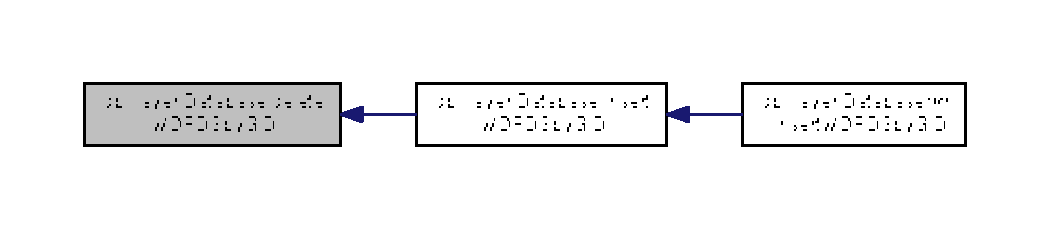
\includegraphics[width=350pt]{classdb__layer_1_1_database_af7c91fdd73898b9e2aa1d1e04ebcb8a6_icgraph}
\end{center}
\end{figure}


\hypertarget{classdb__layer_1_1_database_a8470bd9042a562ac6205dc6edcb374ea}{\index{db\-\_\-layer\-::\-Database@{db\-\_\-layer\-::\-Database}!del\-Group@{del\-Group}}
\index{del\-Group@{del\-Group}!db_layer::Database@{db\-\_\-layer\-::\-Database}}
\subsubsection[{del\-Group}]{\setlength{\rightskip}{0pt plus 5cm}def db\-\_\-layer.\-Database.\-del\-Group (
\begin{DoxyParamCaption}
\item[{}]{self, }
\item[{}]{groupto\-Delete}
\end{DoxyParamCaption}
)}}\label{classdb__layer_1_1_database_a8470bd9042a562ac6205dc6edcb374ea}


Definición en la línea 500 del archivo db\-\_\-layer.\-py.

\hypertarget{classdb__layer_1_1_database_ab4e221a9ae93a5780c084d49d01029d8}{\index{db\-\_\-layer\-::\-Database@{db\-\_\-layer\-::\-Database}!del\-Relation@{del\-Relation}}
\index{del\-Relation@{del\-Relation}!db_layer::Database@{db\-\_\-layer\-::\-Database}}
\subsubsection[{del\-Relation}]{\setlength{\rightskip}{0pt plus 5cm}def db\-\_\-layer.\-Database.\-del\-Relation (
\begin{DoxyParamCaption}
\item[{}]{self, }
\item[{}]{uid, }
\item[{}]{gid}
\end{DoxyParamCaption}
)}}\label{classdb__layer_1_1_database_ab4e221a9ae93a5780c084d49d01029d8}


Definición en la línea 288 del archivo db\-\_\-layer.\-py.



Gráfico de llamadas a esta función\-:\nopagebreak
\begin{figure}[H]
\begin{center}
\leavevmode
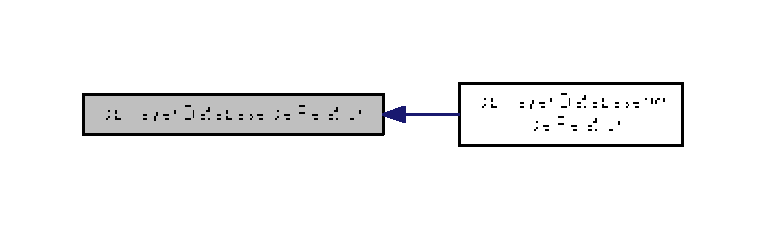
\includegraphics[width=350pt]{classdb__layer_1_1_database_ab4e221a9ae93a5780c084d49d01029d8_icgraph}
\end{center}
\end{figure}


\hypertarget{classdb__layer_1_1_database_ad8447f580fdb6dc37c23fe4220ee62b9}{\index{db\-\_\-layer\-::\-Database@{db\-\_\-layer\-::\-Database}!del\-User@{del\-User}}
\index{del\-User@{del\-User}!db_layer::Database@{db\-\_\-layer\-::\-Database}}
\subsubsection[{del\-User}]{\setlength{\rightskip}{0pt plus 5cm}def db\-\_\-layer.\-Database.\-del\-User (
\begin{DoxyParamCaption}
\item[{}]{self, }
\item[{}]{userto\-Delete}
\end{DoxyParamCaption}
)}}\label{classdb__layer_1_1_database_ad8447f580fdb6dc37c23fe4220ee62b9}


Definición en la línea 308 del archivo db\-\_\-layer.\-py.

\hypertarget{classdb__layer_1_1_database_a39d62bdcc06c57e3a02aa86c31a45f8d}{\index{db\-\_\-layer\-::\-Database@{db\-\_\-layer\-::\-Database}!find\-Group@{find\-Group}}
\index{find\-Group@{find\-Group}!db_layer::Database@{db\-\_\-layer\-::\-Database}}
\subsubsection[{find\-Group}]{\setlength{\rightskip}{0pt plus 5cm}def db\-\_\-layer.\-Database.\-find\-Group (
\begin{DoxyParamCaption}
\item[{}]{self, }
\item[{}]{str2find}
\end{DoxyParamCaption}
)}}\label{classdb__layer_1_1_database_a39d62bdcc06c57e3a02aa86c31a45f8d}


Definición en la línea 462 del archivo db\-\_\-layer.\-py.

\hypertarget{classdb__layer_1_1_database_a16008b08c96fa493d7ee12b2a7a5b181}{\index{db\-\_\-layer\-::\-Database@{db\-\_\-layer\-::\-Database}!find\-Group\-By\-G\-I\-D@{find\-Group\-By\-G\-I\-D}}
\index{find\-Group\-By\-G\-I\-D@{find\-Group\-By\-G\-I\-D}!db_layer::Database@{db\-\_\-layer\-::\-Database}}
\subsubsection[{find\-Group\-By\-G\-I\-D}]{\setlength{\rightskip}{0pt plus 5cm}def db\-\_\-layer.\-Database.\-find\-Group\-By\-G\-I\-D (
\begin{DoxyParamCaption}
\item[{}]{self, }
\item[{}]{gid}
\end{DoxyParamCaption}
)}}\label{classdb__layer_1_1_database_a16008b08c96fa493d7ee12b2a7a5b181}


Definición en la línea 491 del archivo db\-\_\-layer.\-py.



Gráfico de llamadas a esta función\-:\nopagebreak
\begin{figure}[H]
\begin{center}
\leavevmode
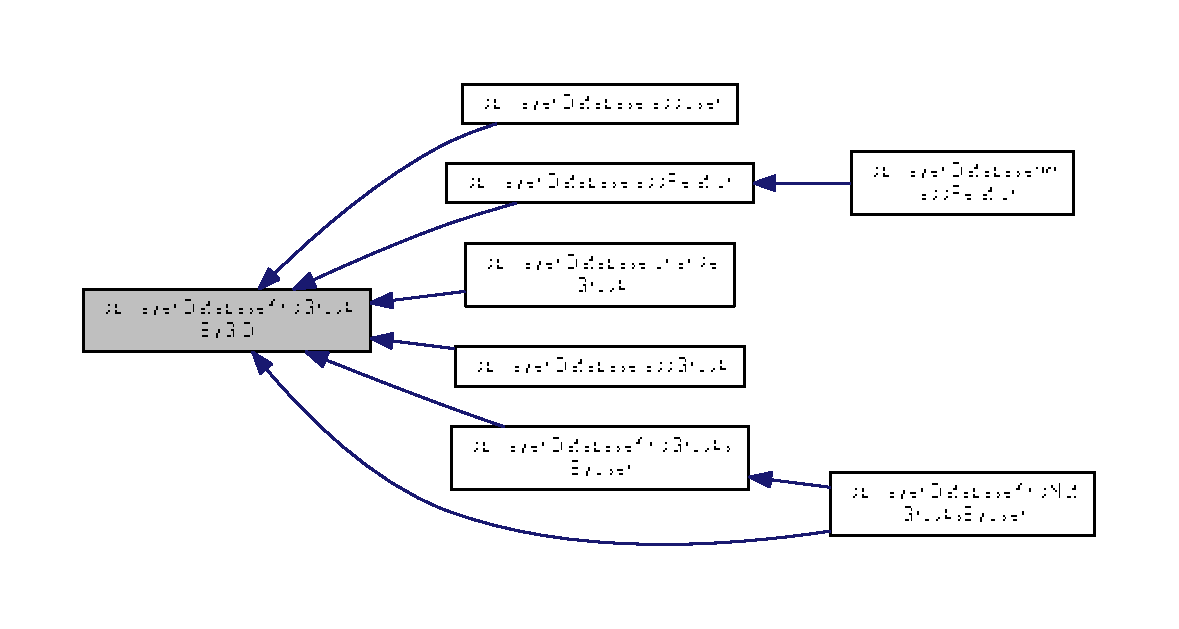
\includegraphics[width=350pt]{classdb__layer_1_1_database_a16008b08c96fa493d7ee12b2a7a5b181_icgraph}
\end{center}
\end{figure}


\hypertarget{classdb__layer_1_1_database_a20c7dd43617755b5ebaf0e1d22a4a2f8}{\index{db\-\_\-layer\-::\-Database@{db\-\_\-layer\-::\-Database}!find\-Group\-By\-Groupname@{find\-Group\-By\-Groupname}}
\index{find\-Group\-By\-Groupname@{find\-Group\-By\-Groupname}!db_layer::Database@{db\-\_\-layer\-::\-Database}}
\subsubsection[{find\-Group\-By\-Groupname}]{\setlength{\rightskip}{0pt plus 5cm}def db\-\_\-layer.\-Database.\-find\-Group\-By\-Groupname (
\begin{DoxyParamCaption}
\item[{}]{self, }
\item[{}]{groupname}
\end{DoxyParamCaption}
)}}\label{classdb__layer_1_1_database_a20c7dd43617755b5ebaf0e1d22a4a2f8}


Definición en la línea 482 del archivo db\-\_\-layer.\-py.



Gráfico de llamadas a esta función\-:\nopagebreak
\begin{figure}[H]
\begin{center}
\leavevmode
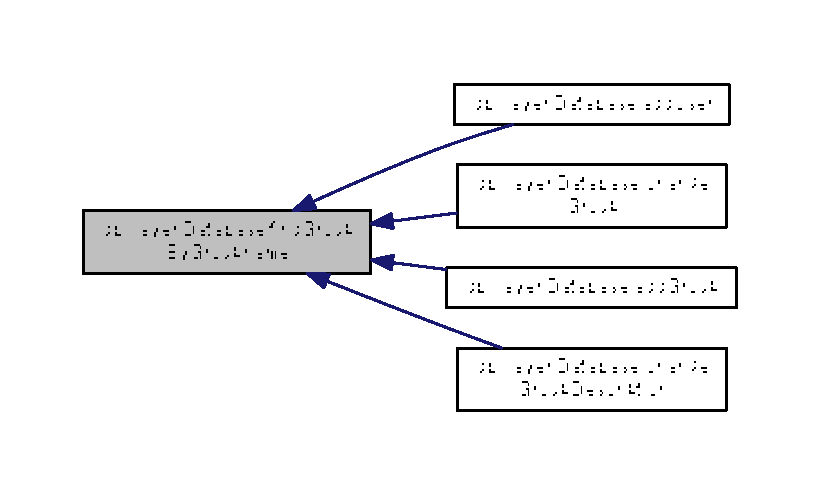
\includegraphics[width=350pt]{classdb__layer_1_1_database_a20c7dd43617755b5ebaf0e1d22a4a2f8_icgraph}
\end{center}
\end{figure}


\hypertarget{classdb__layer_1_1_database_acf2271857a561c1e17069068f5c7e317}{\index{db\-\_\-layer\-::\-Database@{db\-\_\-layer\-::\-Database}!find\-Groups\-By\-User@{find\-Groups\-By\-User}}
\index{find\-Groups\-By\-User@{find\-Groups\-By\-User}!db_layer::Database@{db\-\_\-layer\-::\-Database}}
\subsubsection[{find\-Groups\-By\-User}]{\setlength{\rightskip}{0pt plus 5cm}def db\-\_\-layer.\-Database.\-find\-Groups\-By\-User (
\begin{DoxyParamCaption}
\item[{}]{self, }
\item[{}]{username}
\end{DoxyParamCaption}
)}}\label{classdb__layer_1_1_database_acf2271857a561c1e17069068f5c7e317}


Definición en la línea 703 del archivo db\-\_\-layer.\-py.



Gráfico de llamadas para esta función\-:\nopagebreak
\begin{figure}[H]
\begin{center}
\leavevmode
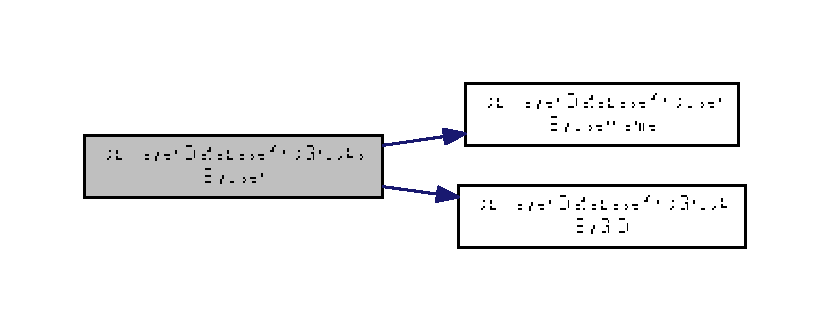
\includegraphics[width=350pt]{classdb__layer_1_1_database_acf2271857a561c1e17069068f5c7e317_cgraph}
\end{center}
\end{figure}




Gráfico de llamadas a esta función\-:\nopagebreak
\begin{figure}[H]
\begin{center}
\leavevmode
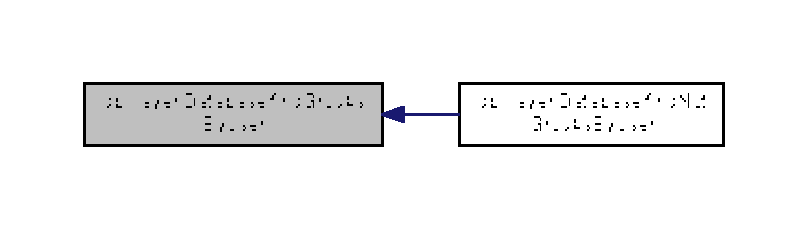
\includegraphics[width=350pt]{classdb__layer_1_1_database_acf2271857a561c1e17069068f5c7e317_icgraph}
\end{center}
\end{figure}


\hypertarget{classdb__layer_1_1_database_a940f5d9df2aa98c4c4452d9a005a0788}{\index{db\-\_\-layer\-::\-Database@{db\-\_\-layer\-::\-Database}!find\-M\-I\-M\-E\-Sby\-G\-I\-D@{find\-M\-I\-M\-E\-Sby\-G\-I\-D}}
\index{find\-M\-I\-M\-E\-Sby\-G\-I\-D@{find\-M\-I\-M\-E\-Sby\-G\-I\-D}!db_layer::Database@{db\-\_\-layer\-::\-Database}}
\subsubsection[{find\-M\-I\-M\-E\-Sby\-G\-I\-D}]{\setlength{\rightskip}{0pt plus 5cm}def db\-\_\-layer.\-Database.\-find\-M\-I\-M\-E\-Sby\-G\-I\-D (
\begin{DoxyParamCaption}
\item[{}]{self, }
\item[{}]{gid}
\end{DoxyParamCaption}
)}}\label{classdb__layer_1_1_database_a940f5d9df2aa98c4c4452d9a005a0788}


Definición en la línea 845 del archivo db\-\_\-layer.\-py.



Gráfico de llamadas a esta función\-:\nopagebreak
\begin{figure}[H]
\begin{center}
\leavevmode
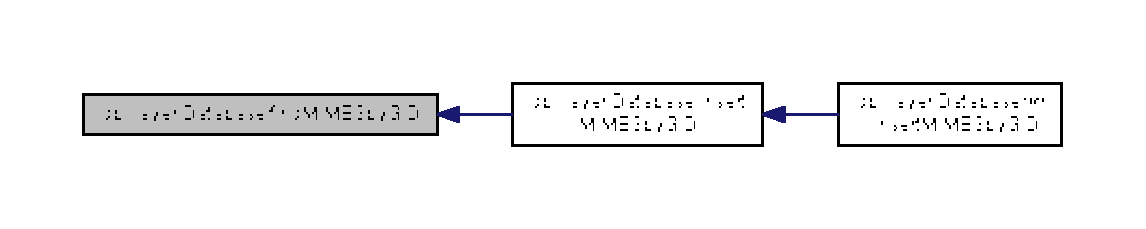
\includegraphics[width=350pt]{classdb__layer_1_1_database_a940f5d9df2aa98c4c4452d9a005a0788_icgraph}
\end{center}
\end{figure}


\hypertarget{classdb__layer_1_1_database_a782bfdf0a4415ef9f520722125851924}{\index{db\-\_\-layer\-::\-Database@{db\-\_\-layer\-::\-Database}!find\-Not\-Groups\-By\-User@{find\-Not\-Groups\-By\-User}}
\index{find\-Not\-Groups\-By\-User@{find\-Not\-Groups\-By\-User}!db_layer::Database@{db\-\_\-layer\-::\-Database}}
\subsubsection[{find\-Not\-Groups\-By\-User}]{\setlength{\rightskip}{0pt plus 5cm}def db\-\_\-layer.\-Database.\-find\-Not\-Groups\-By\-User (
\begin{DoxyParamCaption}
\item[{}]{self, }
\item[{}]{username}
\end{DoxyParamCaption}
)}}\label{classdb__layer_1_1_database_a782bfdf0a4415ef9f520722125851924}


Definición en la línea 729 del archivo db\-\_\-layer.\-py.



Gráfico de llamadas para esta función\-:\nopagebreak
\begin{figure}[H]
\begin{center}
\leavevmode
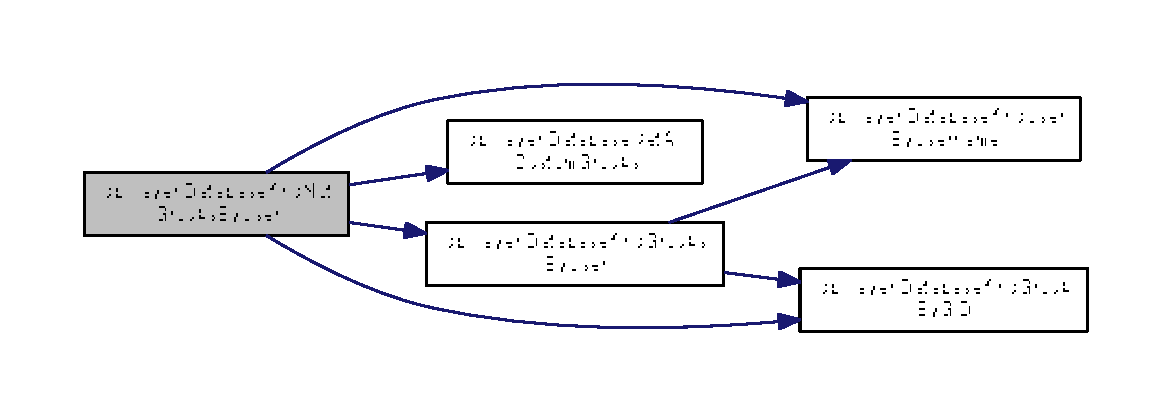
\includegraphics[width=350pt]{classdb__layer_1_1_database_a782bfdf0a4415ef9f520722125851924_cgraph}
\end{center}
\end{figure}


\hypertarget{classdb__layer_1_1_database_abe7e2fc7937e3fd641a8ec5275b4db60}{\index{db\-\_\-layer\-::\-Database@{db\-\_\-layer\-::\-Database}!find\-U\-R\-I\-Sby\-G\-I\-D@{find\-U\-R\-I\-Sby\-G\-I\-D}}
\index{find\-U\-R\-I\-Sby\-G\-I\-D@{find\-U\-R\-I\-Sby\-G\-I\-D}!db_layer::Database@{db\-\_\-layer\-::\-Database}}
\subsubsection[{find\-U\-R\-I\-Sby\-G\-I\-D}]{\setlength{\rightskip}{0pt plus 5cm}def db\-\_\-layer.\-Database.\-find\-U\-R\-I\-Sby\-G\-I\-D (
\begin{DoxyParamCaption}
\item[{}]{self, }
\item[{}]{gid}
\end{DoxyParamCaption}
)}}\label{classdb__layer_1_1_database_abe7e2fc7937e3fd641a8ec5275b4db60}


Definición en la línea 750 del archivo db\-\_\-layer.\-py.



Gráfico de llamadas a esta función\-:\nopagebreak
\begin{figure}[H]
\begin{center}
\leavevmode
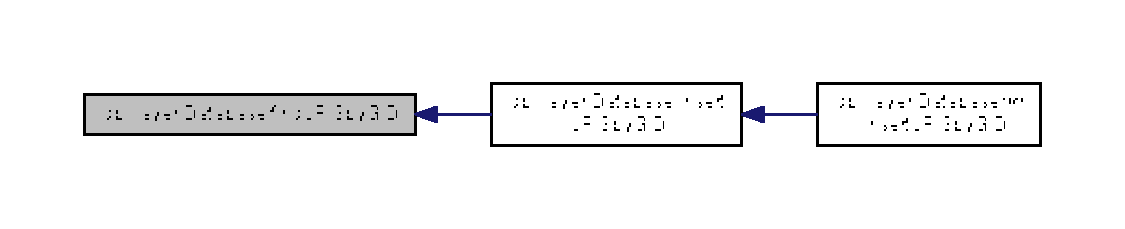
\includegraphics[width=350pt]{classdb__layer_1_1_database_abe7e2fc7937e3fd641a8ec5275b4db60_icgraph}
\end{center}
\end{figure}


\hypertarget{classdb__layer_1_1_database_aaa54107650dc6511c7afdaf98112d4c1}{\index{db\-\_\-layer\-::\-Database@{db\-\_\-layer\-::\-Database}!find\-User@{find\-User}}
\index{find\-User@{find\-User}!db_layer::Database@{db\-\_\-layer\-::\-Database}}
\subsubsection[{find\-User}]{\setlength{\rightskip}{0pt plus 5cm}def db\-\_\-layer.\-Database.\-find\-User (
\begin{DoxyParamCaption}
\item[{}]{self, }
\item[{}]{str2find}
\end{DoxyParamCaption}
)}}\label{classdb__layer_1_1_database_aaa54107650dc6511c7afdaf98112d4c1}


Definición en la línea 125 del archivo db\-\_\-layer.\-py.

\hypertarget{classdb__layer_1_1_database_aa97a7c93c41d97e60600dec9fb87270e}{\index{db\-\_\-layer\-::\-Database@{db\-\_\-layer\-::\-Database}!find\-User\-By\-U\-I\-D@{find\-User\-By\-U\-I\-D}}
\index{find\-User\-By\-U\-I\-D@{find\-User\-By\-U\-I\-D}!db_layer::Database@{db\-\_\-layer\-::\-Database}}
\subsubsection[{find\-User\-By\-U\-I\-D}]{\setlength{\rightskip}{0pt plus 5cm}def db\-\_\-layer.\-Database.\-find\-User\-By\-U\-I\-D (
\begin{DoxyParamCaption}
\item[{}]{self, }
\item[{}]{uid}
\end{DoxyParamCaption}
)}}\label{classdb__layer_1_1_database_aa97a7c93c41d97e60600dec9fb87270e}


Definición en la línea 178 del archivo db\-\_\-layer.\-py.



Gráfico de llamadas a esta función\-:\nopagebreak
\begin{figure}[H]
\begin{center}
\leavevmode
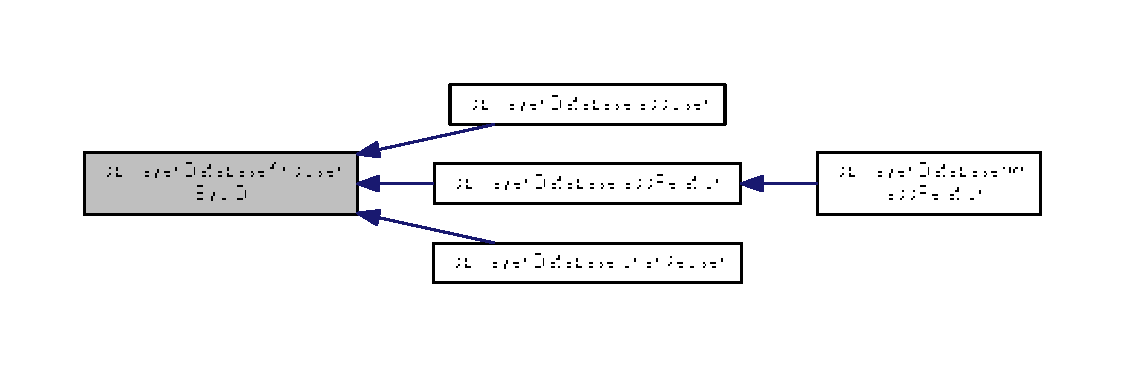
\includegraphics[width=350pt]{classdb__layer_1_1_database_aa97a7c93c41d97e60600dec9fb87270e_icgraph}
\end{center}
\end{figure}


\hypertarget{classdb__layer_1_1_database_a321ec63103a76c21fb556f82bc03e08f}{\index{db\-\_\-layer\-::\-Database@{db\-\_\-layer\-::\-Database}!find\-User\-By\-Username@{find\-User\-By\-Username}}
\index{find\-User\-By\-Username@{find\-User\-By\-Username}!db_layer::Database@{db\-\_\-layer\-::\-Database}}
\subsubsection[{find\-User\-By\-Username}]{\setlength{\rightskip}{0pt plus 5cm}def db\-\_\-layer.\-Database.\-find\-User\-By\-Username (
\begin{DoxyParamCaption}
\item[{}]{self, }
\item[{}]{username}
\end{DoxyParamCaption}
)}}\label{classdb__layer_1_1_database_a321ec63103a76c21fb556f82bc03e08f}


Definición en la línea 146 del archivo db\-\_\-layer.\-py.



Gráfico de llamadas a esta función\-:\nopagebreak
\begin{figure}[H]
\begin{center}
\leavevmode
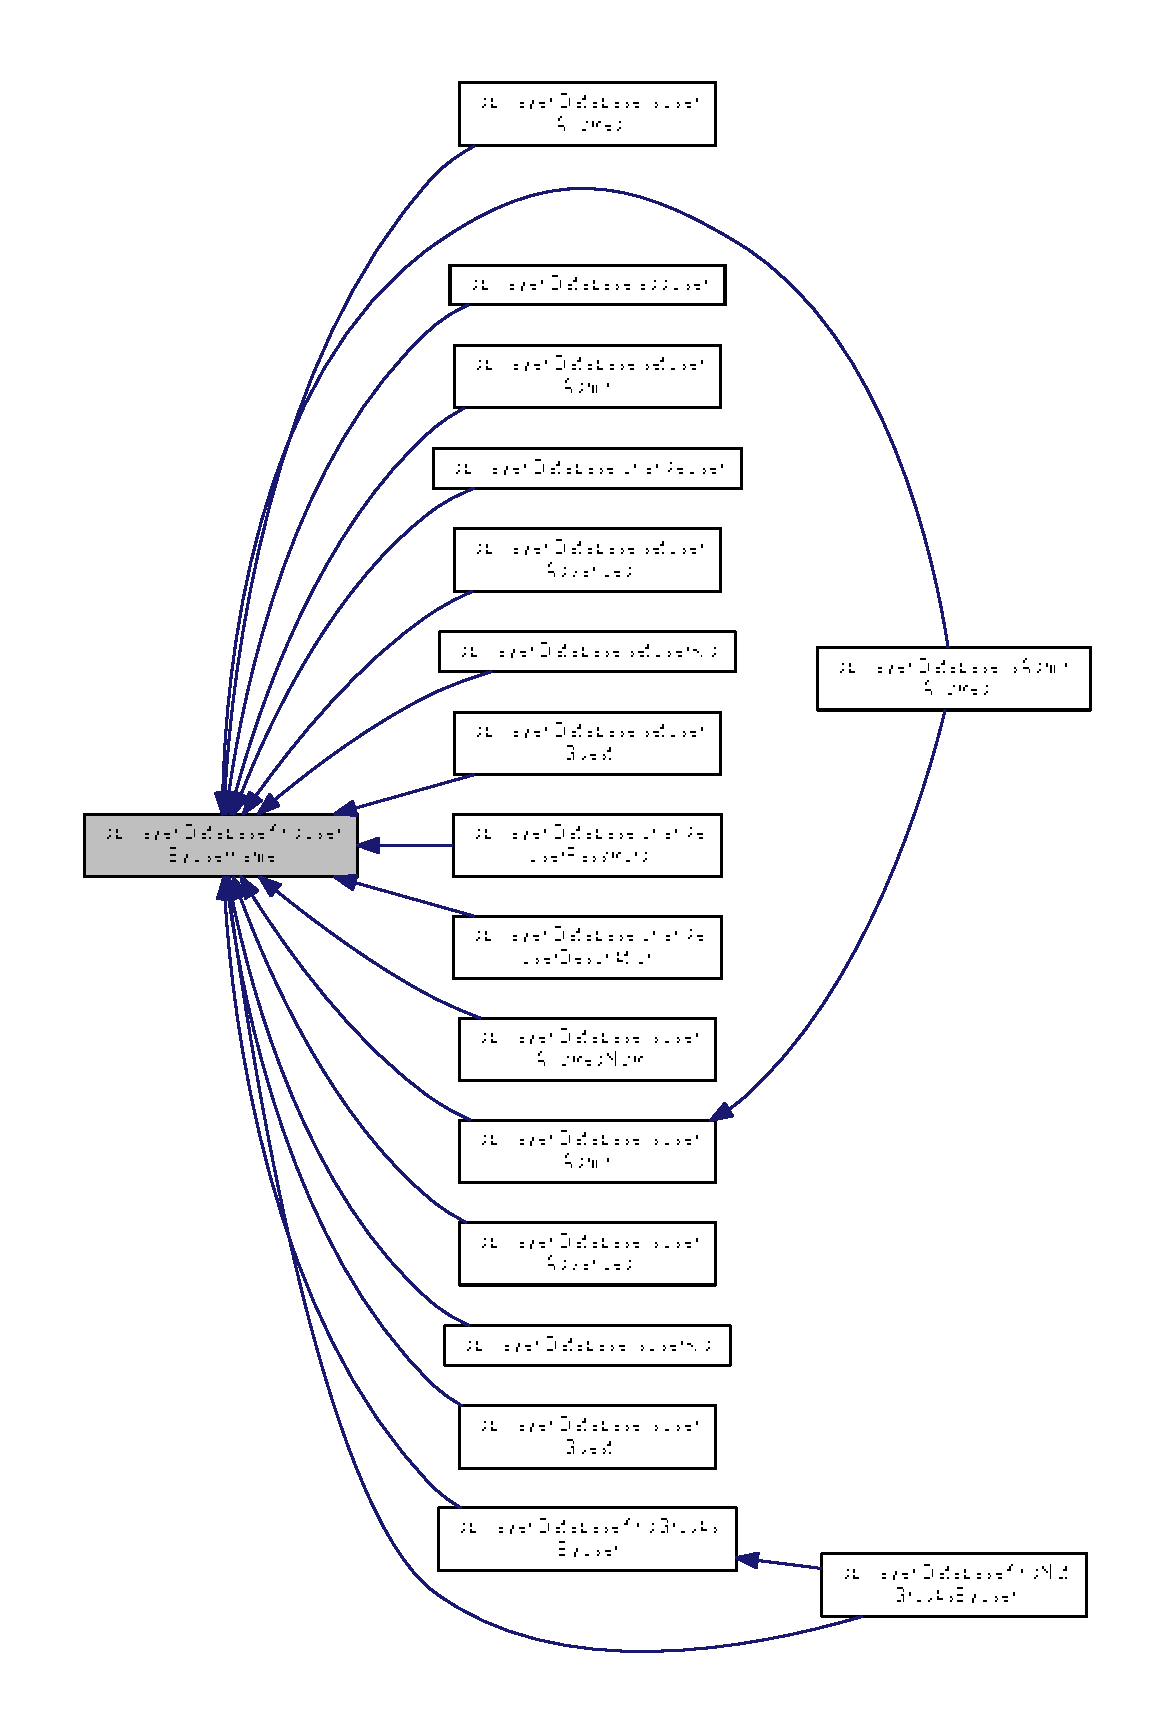
\includegraphics[width=350pt]{classdb__layer_1_1_database_a321ec63103a76c21fb556f82bc03e08f_icgraph}
\end{center}
\end{figure}


\hypertarget{classdb__layer_1_1_database_a7f168024109c6490cca9f764cd0bbeac}{\index{db\-\_\-layer\-::\-Database@{db\-\_\-layer\-::\-Database}!find\-W\-O\-R\-D\-Sby\-G\-I\-D@{find\-W\-O\-R\-D\-Sby\-G\-I\-D}}
\index{find\-W\-O\-R\-D\-Sby\-G\-I\-D@{find\-W\-O\-R\-D\-Sby\-G\-I\-D}!db_layer::Database@{db\-\_\-layer\-::\-Database}}
\subsubsection[{find\-W\-O\-R\-D\-Sby\-G\-I\-D}]{\setlength{\rightskip}{0pt plus 5cm}def db\-\_\-layer.\-Database.\-find\-W\-O\-R\-D\-Sby\-G\-I\-D (
\begin{DoxyParamCaption}
\item[{}]{self, }
\item[{}]{gid}
\end{DoxyParamCaption}
)}}\label{classdb__layer_1_1_database_a7f168024109c6490cca9f764cd0bbeac}


Definición en la línea 800 del archivo db\-\_\-layer.\-py.



Gráfico de llamadas a esta función\-:\nopagebreak
\begin{figure}[H]
\begin{center}
\leavevmode
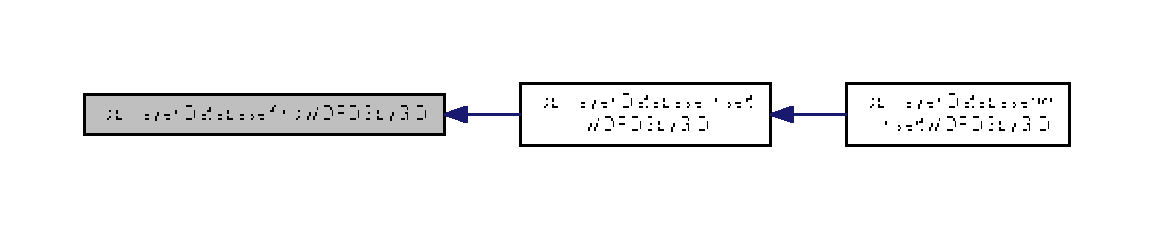
\includegraphics[width=350pt]{classdb__layer_1_1_database_a7f168024109c6490cca9f764cd0bbeac_icgraph}
\end{center}
\end{figure}


\hypertarget{classdb__layer_1_1_database_a22ed5c7f36dbb61e6f60c4040987bf55}{\index{db\-\_\-layer\-::\-Database@{db\-\_\-layer\-::\-Database}!get\-All\-Custom\-Groups@{get\-All\-Custom\-Groups}}
\index{get\-All\-Custom\-Groups@{get\-All\-Custom\-Groups}!db_layer::Database@{db\-\_\-layer\-::\-Database}}
\subsubsection[{get\-All\-Custom\-Groups}]{\setlength{\rightskip}{0pt plus 5cm}def db\-\_\-layer.\-Database.\-get\-All\-Custom\-Groups (
\begin{DoxyParamCaption}
\item[{}]{self}
\end{DoxyParamCaption}
)}}\label{classdb__layer_1_1_database_a22ed5c7f36dbb61e6f60c4040987bf55}


Definición en la línea 541 del archivo db\-\_\-layer.\-py.



Gráfico de llamadas a esta función\-:\nopagebreak
\begin{figure}[H]
\begin{center}
\leavevmode
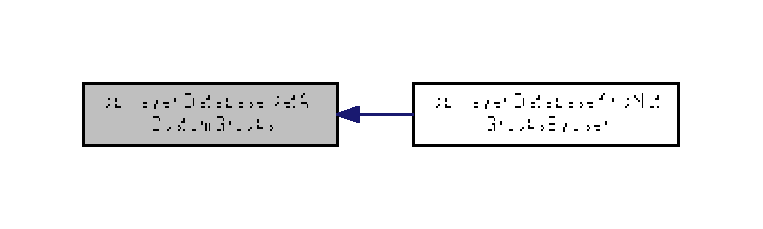
\includegraphics[width=350pt]{classdb__layer_1_1_database_a22ed5c7f36dbb61e6f60c4040987bf55_icgraph}
\end{center}
\end{figure}


\hypertarget{classdb__layer_1_1_database_aec26922467f83a27ddc41b583f0f1cb0}{\index{db\-\_\-layer\-::\-Database@{db\-\_\-layer\-::\-Database}!get\-All\-Groups@{get\-All\-Groups}}
\index{get\-All\-Groups@{get\-All\-Groups}!db_layer::Database@{db\-\_\-layer\-::\-Database}}
\subsubsection[{get\-All\-Groups}]{\setlength{\rightskip}{0pt plus 5cm}def db\-\_\-layer.\-Database.\-get\-All\-Groups (
\begin{DoxyParamCaption}
\item[{}]{self}
\end{DoxyParamCaption}
)}}\label{classdb__layer_1_1_database_aec26922467f83a27ddc41b583f0f1cb0}


Definición en la línea 535 del archivo db\-\_\-layer.\-py.

\hypertarget{classdb__layer_1_1_database_aa56ec835e0baf06452952528e12062bc}{\index{db\-\_\-layer\-::\-Database@{db\-\_\-layer\-::\-Database}!get\-All\-User@{get\-All\-User}}
\index{get\-All\-User@{get\-All\-User}!db_layer::Database@{db\-\_\-layer\-::\-Database}}
\subsubsection[{get\-All\-User}]{\setlength{\rightskip}{0pt plus 5cm}def db\-\_\-layer.\-Database.\-get\-All\-User (
\begin{DoxyParamCaption}
\item[{}]{self}
\end{DoxyParamCaption}
)}}\label{classdb__layer_1_1_database_aa56ec835e0baf06452952528e12062bc}


Definición en la línea 188 del archivo db\-\_\-layer.\-py.

\hypertarget{classdb__layer_1_1_database_a98fa2d3a8377bca1fe5f2d2946ef2929}{\index{db\-\_\-layer\-::\-Database@{db\-\_\-layer\-::\-Database}!get\-Lowest\-Unused\-G\-I\-Dfrom\-Group@{get\-Lowest\-Unused\-G\-I\-Dfrom\-Group}}
\index{get\-Lowest\-Unused\-G\-I\-Dfrom\-Group@{get\-Lowest\-Unused\-G\-I\-Dfrom\-Group}!db_layer::Database@{db\-\_\-layer\-::\-Database}}
\subsubsection[{get\-Lowest\-Unused\-G\-I\-Dfrom\-Group}]{\setlength{\rightskip}{0pt plus 5cm}def db\-\_\-layer.\-Database.\-get\-Lowest\-Unused\-G\-I\-Dfrom\-Group (
\begin{DoxyParamCaption}
\item[{}]{self}
\end{DoxyParamCaption}
)}}\label{classdb__layer_1_1_database_a98fa2d3a8377bca1fe5f2d2946ef2929}


Definición en la línea 550 del archivo db\-\_\-layer.\-py.



Gráfico de llamadas a esta función\-:\nopagebreak
\begin{figure}[H]
\begin{center}
\leavevmode
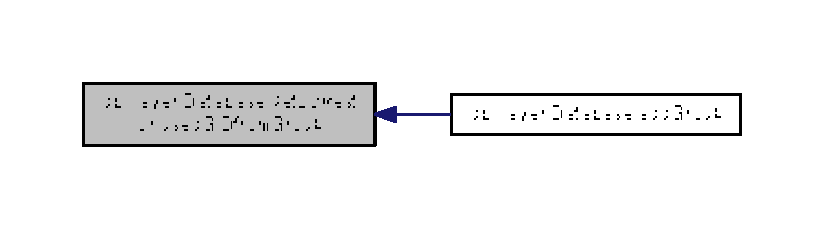
\includegraphics[width=350pt]{classdb__layer_1_1_database_a98fa2d3a8377bca1fe5f2d2946ef2929_icgraph}
\end{center}
\end{figure}


\hypertarget{classdb__layer_1_1_database_a99ba044bb2e8692e27c34b74f6420ce8}{\index{db\-\_\-layer\-::\-Database@{db\-\_\-layer\-::\-Database}!get\-Lowest\-Unused\-U\-I\-Dfrom\-User@{get\-Lowest\-Unused\-U\-I\-Dfrom\-User}}
\index{get\-Lowest\-Unused\-U\-I\-Dfrom\-User@{get\-Lowest\-Unused\-U\-I\-Dfrom\-User}!db_layer::Database@{db\-\_\-layer\-::\-Database}}
\subsubsection[{get\-Lowest\-Unused\-U\-I\-Dfrom\-User}]{\setlength{\rightskip}{0pt plus 5cm}def db\-\_\-layer.\-Database.\-get\-Lowest\-Unused\-U\-I\-Dfrom\-User (
\begin{DoxyParamCaption}
\item[{}]{self}
\end{DoxyParamCaption}
)}}\label{classdb__layer_1_1_database_a99ba044bb2e8692e27c34b74f6420ce8}


Definición en la línea 196 del archivo db\-\_\-layer.\-py.



Gráfico de llamadas a esta función\-:\nopagebreak
\begin{figure}[H]
\begin{center}
\leavevmode
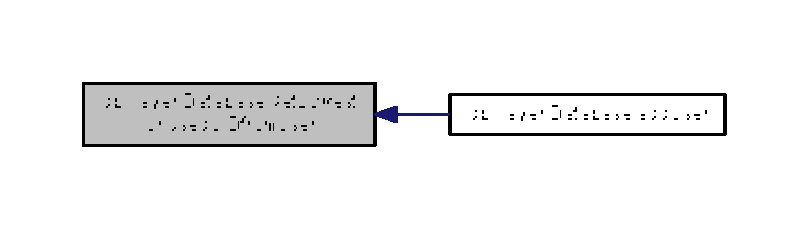
\includegraphics[width=350pt]{classdb__layer_1_1_database_a99ba044bb2e8692e27c34b74f6420ce8_icgraph}
\end{center}
\end{figure}


\hypertarget{classdb__layer_1_1_database_a014383f7f432ef974c12c87bdbe08546}{\index{db\-\_\-layer\-::\-Database@{db\-\_\-layer\-::\-Database}!get\-R\-U\-L\-E\-S@{get\-R\-U\-L\-E\-S}}
\index{get\-R\-U\-L\-E\-S@{get\-R\-U\-L\-E\-S}!db_layer::Database@{db\-\_\-layer\-::\-Database}}
\subsubsection[{get\-R\-U\-L\-E\-S}]{\setlength{\rightskip}{0pt plus 5cm}def db\-\_\-layer.\-Database.\-get\-R\-U\-L\-E\-S (
\begin{DoxyParamCaption}
\item[{}]{self, }
\item[{}]{kind, }
\item[{}]{username}
\end{DoxyParamCaption}
)}}\label{classdb__layer_1_1_database_a014383f7f432ef974c12c87bdbe08546}


Definición en la línea 891 del archivo db\-\_\-layer.\-py.

\hypertarget{classdb__layer_1_1_database_ae95955bc5ae21324a753dca4d76f69f1}{\index{db\-\_\-layer\-::\-Database@{db\-\_\-layer\-::\-Database}!insert\-M\-I\-M\-E\-Sby\-G\-I\-D@{insert\-M\-I\-M\-E\-Sby\-G\-I\-D}}
\index{insert\-M\-I\-M\-E\-Sby\-G\-I\-D@{insert\-M\-I\-M\-E\-Sby\-G\-I\-D}!db_layer::Database@{db\-\_\-layer\-::\-Database}}
\subsubsection[{insert\-M\-I\-M\-E\-Sby\-G\-I\-D}]{\setlength{\rightskip}{0pt plus 5cm}def db\-\_\-layer.\-Database.\-insert\-M\-I\-M\-E\-Sby\-G\-I\-D (
\begin{DoxyParamCaption}
\item[{}]{self, }
\item[{}]{gid, }
\item[{}]{data}
\end{DoxyParamCaption}
)}}\label{classdb__layer_1_1_database_ae95955bc5ae21324a753dca4d76f69f1}


Definición en la línea 863 del archivo db\-\_\-layer.\-py.



Gráfico de llamadas para esta función\-:\nopagebreak
\begin{figure}[H]
\begin{center}
\leavevmode
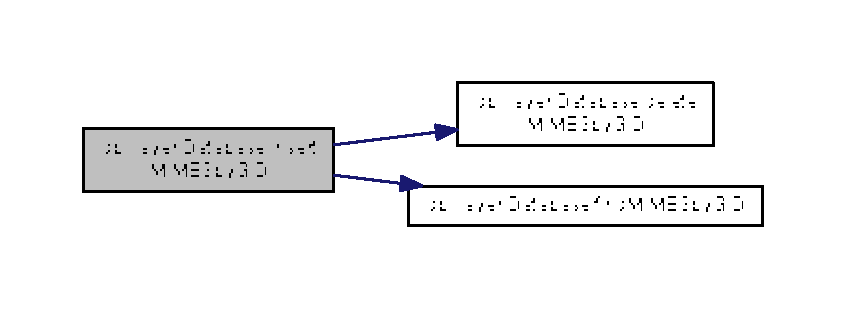
\includegraphics[width=350pt]{classdb__layer_1_1_database_ae95955bc5ae21324a753dca4d76f69f1_cgraph}
\end{center}
\end{figure}




Gráfico de llamadas a esta función\-:\nopagebreak
\begin{figure}[H]
\begin{center}
\leavevmode
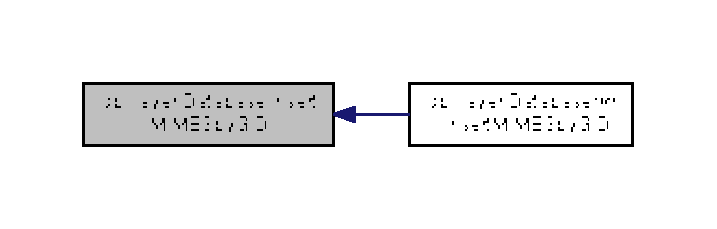
\includegraphics[width=344pt]{classdb__layer_1_1_database_ae95955bc5ae21324a753dca4d76f69f1_icgraph}
\end{center}
\end{figure}


\hypertarget{classdb__layer_1_1_database_aebc7fd132c862539ede9959fa4257d2a}{\index{db\-\_\-layer\-::\-Database@{db\-\_\-layer\-::\-Database}!insert\-U\-R\-I\-Sby\-G\-I\-D@{insert\-U\-R\-I\-Sby\-G\-I\-D}}
\index{insert\-U\-R\-I\-Sby\-G\-I\-D@{insert\-U\-R\-I\-Sby\-G\-I\-D}!db_layer::Database@{db\-\_\-layer\-::\-Database}}
\subsubsection[{insert\-U\-R\-I\-Sby\-G\-I\-D}]{\setlength{\rightskip}{0pt plus 5cm}def db\-\_\-layer.\-Database.\-insert\-U\-R\-I\-Sby\-G\-I\-D (
\begin{DoxyParamCaption}
\item[{}]{self, }
\item[{}]{gid, }
\item[{}]{data}
\end{DoxyParamCaption}
)}}\label{classdb__layer_1_1_database_aebc7fd132c862539ede9959fa4257d2a}


Definición en la línea 771 del archivo db\-\_\-layer.\-py.



Gráfico de llamadas para esta función\-:\nopagebreak
\begin{figure}[H]
\begin{center}
\leavevmode
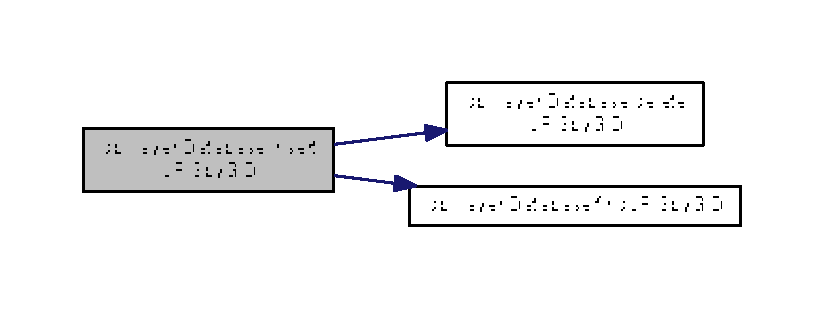
\includegraphics[width=350pt]{classdb__layer_1_1_database_aebc7fd132c862539ede9959fa4257d2a_cgraph}
\end{center}
\end{figure}




Gráfico de llamadas a esta función\-:\nopagebreak
\begin{figure}[H]
\begin{center}
\leavevmode
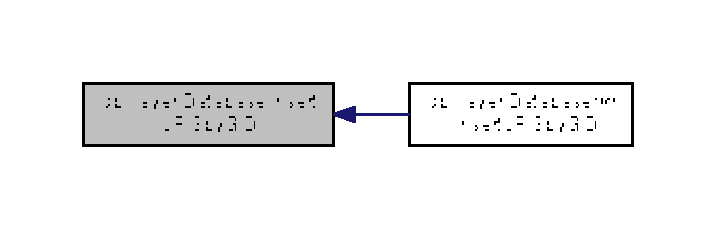
\includegraphics[width=344pt]{classdb__layer_1_1_database_aebc7fd132c862539ede9959fa4257d2a_icgraph}
\end{center}
\end{figure}


\hypertarget{classdb__layer_1_1_database_a849faf2993ee0d75f38639f22c3553e7}{\index{db\-\_\-layer\-::\-Database@{db\-\_\-layer\-::\-Database}!insert\-W\-O\-R\-D\-Sby\-G\-I\-D@{insert\-W\-O\-R\-D\-Sby\-G\-I\-D}}
\index{insert\-W\-O\-R\-D\-Sby\-G\-I\-D@{insert\-W\-O\-R\-D\-Sby\-G\-I\-D}!db_layer::Database@{db\-\_\-layer\-::\-Database}}
\subsubsection[{insert\-W\-O\-R\-D\-Sby\-G\-I\-D}]{\setlength{\rightskip}{0pt plus 5cm}def db\-\_\-layer.\-Database.\-insert\-W\-O\-R\-D\-Sby\-G\-I\-D (
\begin{DoxyParamCaption}
\item[{}]{self, }
\item[{}]{gid, }
\item[{}]{data}
\end{DoxyParamCaption}
)}}\label{classdb__layer_1_1_database_a849faf2993ee0d75f38639f22c3553e7}


Definición en la línea 818 del archivo db\-\_\-layer.\-py.



Gráfico de llamadas para esta función\-:\nopagebreak
\begin{figure}[H]
\begin{center}
\leavevmode
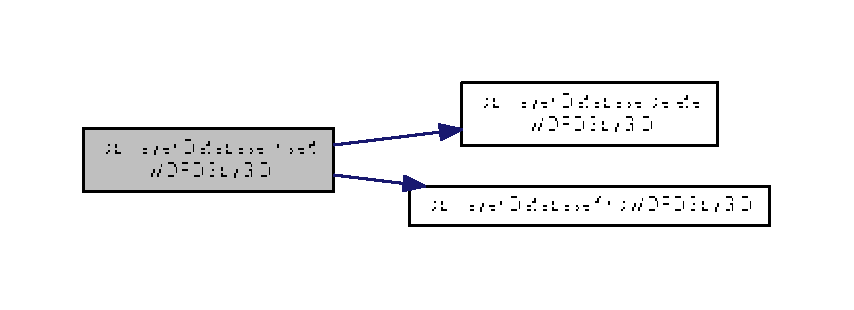
\includegraphics[width=350pt]{classdb__layer_1_1_database_a849faf2993ee0d75f38639f22c3553e7_cgraph}
\end{center}
\end{figure}




Gráfico de llamadas a esta función\-:\nopagebreak
\begin{figure}[H]
\begin{center}
\leavevmode
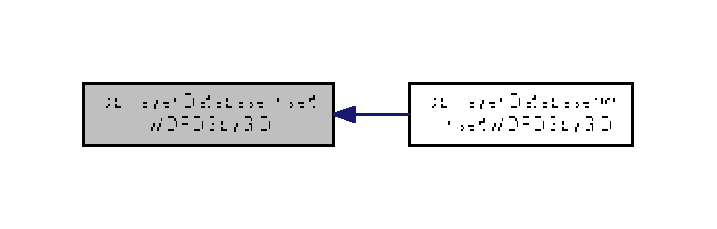
\includegraphics[width=344pt]{classdb__layer_1_1_database_a849faf2993ee0d75f38639f22c3553e7_icgraph}
\end{center}
\end{figure}


\hypertarget{classdb__layer_1_1_database_a1f4a9b4e8dbd15d9f0ce74c1464ec3f9}{\index{db\-\_\-layer\-::\-Database@{db\-\_\-layer\-::\-Database}!is\-Admin\-Allowed@{is\-Admin\-Allowed}}
\index{is\-Admin\-Allowed@{is\-Admin\-Allowed}!db_layer::Database@{db\-\_\-layer\-::\-Database}}
\subsubsection[{is\-Admin\-Allowed}]{\setlength{\rightskip}{0pt plus 5cm}def db\-\_\-layer.\-Database.\-is\-Admin\-Allowed (
\begin{DoxyParamCaption}
\item[{}]{self, }
\item[{}]{username, }
\item[{}]{password}
\end{DoxyParamCaption}
)}}\label{classdb__layer_1_1_database_a1f4a9b4e8dbd15d9f0ce74c1464ec3f9}


Definición en la línea 166 del archivo db\-\_\-layer.\-py.



Gráfico de llamadas para esta función\-:\nopagebreak
\begin{figure}[H]
\begin{center}
\leavevmode
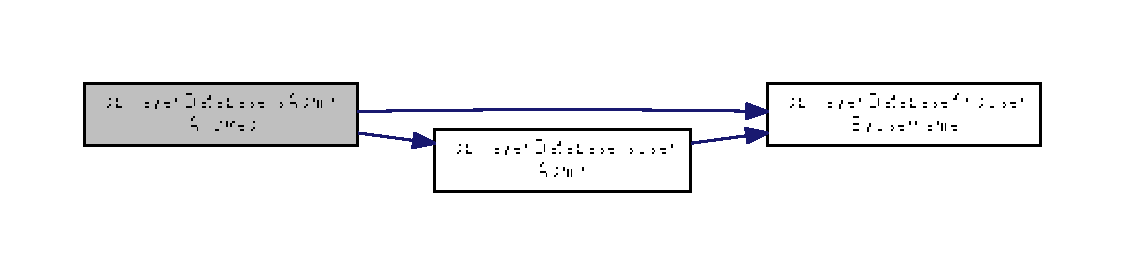
\includegraphics[width=350pt]{classdb__layer_1_1_database_a1f4a9b4e8dbd15d9f0ce74c1464ec3f9_cgraph}
\end{center}
\end{figure}


\hypertarget{classdb__layer_1_1_database_a9ddac6b8ec475ecd6e817329416e3d22}{\index{db\-\_\-layer\-::\-Database@{db\-\_\-layer\-::\-Database}!is\-User\-Admin@{is\-User\-Admin}}
\index{is\-User\-Admin@{is\-User\-Admin}!db_layer::Database@{db\-\_\-layer\-::\-Database}}
\subsubsection[{is\-User\-Admin}]{\setlength{\rightskip}{0pt plus 5cm}def db\-\_\-layer.\-Database.\-is\-User\-Admin (
\begin{DoxyParamCaption}
\item[{}]{self, }
\item[{}]{username}
\end{DoxyParamCaption}
)}}\label{classdb__layer_1_1_database_a9ddac6b8ec475ecd6e817329416e3d22}


Definición en la línea 655 del archivo db\-\_\-layer.\-py.



Gráfico de llamadas para esta función\-:\nopagebreak
\begin{figure}[H]
\begin{center}
\leavevmode
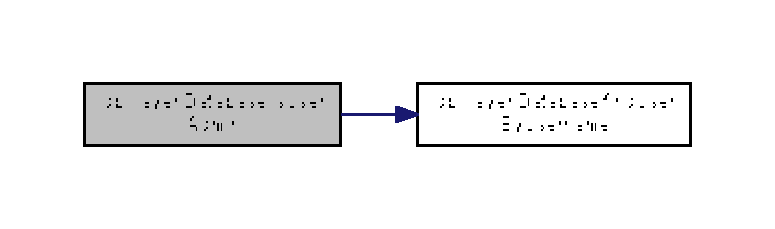
\includegraphics[width=350pt]{classdb__layer_1_1_database_a9ddac6b8ec475ecd6e817329416e3d22_cgraph}
\end{center}
\end{figure}




Gráfico de llamadas a esta función\-:\nopagebreak
\begin{figure}[H]
\begin{center}
\leavevmode
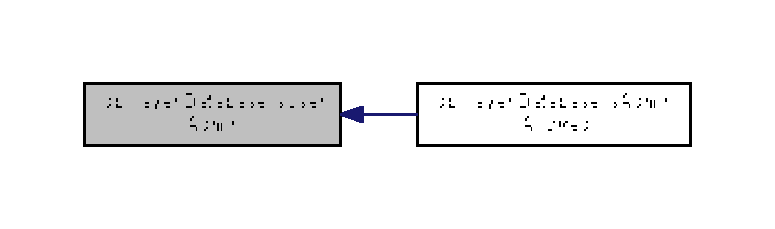
\includegraphics[width=350pt]{classdb__layer_1_1_database_a9ddac6b8ec475ecd6e817329416e3d22_icgraph}
\end{center}
\end{figure}


\hypertarget{classdb__layer_1_1_database_abbe6297269170e88f0ebe7da784fb62b}{\index{db\-\_\-layer\-::\-Database@{db\-\_\-layer\-::\-Database}!is\-User\-Advanced@{is\-User\-Advanced}}
\index{is\-User\-Advanced@{is\-User\-Advanced}!db_layer::Database@{db\-\_\-layer\-::\-Database}}
\subsubsection[{is\-User\-Advanced}]{\setlength{\rightskip}{0pt plus 5cm}def db\-\_\-layer.\-Database.\-is\-User\-Advanced (
\begin{DoxyParamCaption}
\item[{}]{self, }
\item[{}]{username}
\end{DoxyParamCaption}
)}}\label{classdb__layer_1_1_database_abbe6297269170e88f0ebe7da784fb62b}


Definición en la línea 667 del archivo db\-\_\-layer.\-py.



Gráfico de llamadas para esta función\-:\nopagebreak
\begin{figure}[H]
\begin{center}
\leavevmode
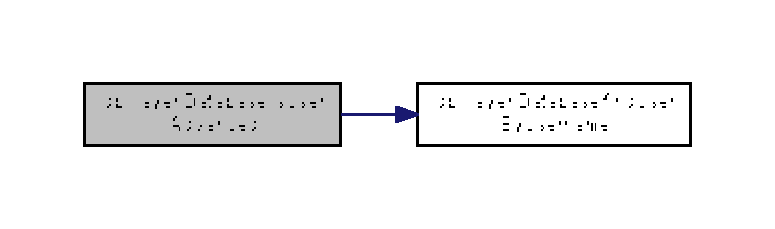
\includegraphics[width=350pt]{classdb__layer_1_1_database_abbe6297269170e88f0ebe7da784fb62b_cgraph}
\end{center}
\end{figure}


\hypertarget{classdb__layer_1_1_database_a738e07ff3b7292931bb057d174866249}{\index{db\-\_\-layer\-::\-Database@{db\-\_\-layer\-::\-Database}!is\-User\-Allowed@{is\-User\-Allowed}}
\index{is\-User\-Allowed@{is\-User\-Allowed}!db_layer::Database@{db\-\_\-layer\-::\-Database}}
\subsubsection[{is\-User\-Allowed}]{\setlength{\rightskip}{0pt plus 5cm}def db\-\_\-layer.\-Database.\-is\-User\-Allowed (
\begin{DoxyParamCaption}
\item[{}]{self, }
\item[{}]{username, }
\item[{}]{password}
\end{DoxyParamCaption}
)}}\label{classdb__layer_1_1_database_a738e07ff3b7292931bb057d174866249}


Definición en la línea 156 del archivo db\-\_\-layer.\-py.



Gráfico de llamadas para esta función\-:\nopagebreak
\begin{figure}[H]
\begin{center}
\leavevmode
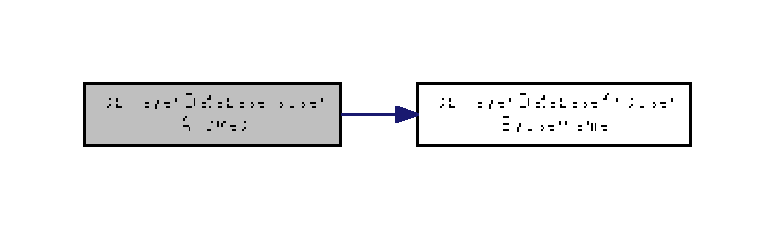
\includegraphics[width=350pt]{classdb__layer_1_1_database_a738e07ff3b7292931bb057d174866249_cgraph}
\end{center}
\end{figure}


\hypertarget{classdb__layer_1_1_database_af6ba4fcf6bcd589b0c85b05f49f46ef5}{\index{db\-\_\-layer\-::\-Database@{db\-\_\-layer\-::\-Database}!is\-User\-Allowed\-Now@{is\-User\-Allowed\-Now}}
\index{is\-User\-Allowed\-Now@{is\-User\-Allowed\-Now}!db_layer::Database@{db\-\_\-layer\-::\-Database}}
\subsubsection[{is\-User\-Allowed\-Now}]{\setlength{\rightskip}{0pt plus 5cm}def db\-\_\-layer.\-Database.\-is\-User\-Allowed\-Now (
\begin{DoxyParamCaption}
\item[{}]{self, }
\item[{}]{username}
\end{DoxyParamCaption}
)}}\label{classdb__layer_1_1_database_af6ba4fcf6bcd589b0c85b05f49f46ef5}


Definición en la línea 605 del archivo db\-\_\-layer.\-py.



Gráfico de llamadas para esta función\-:\nopagebreak
\begin{figure}[H]
\begin{center}
\leavevmode
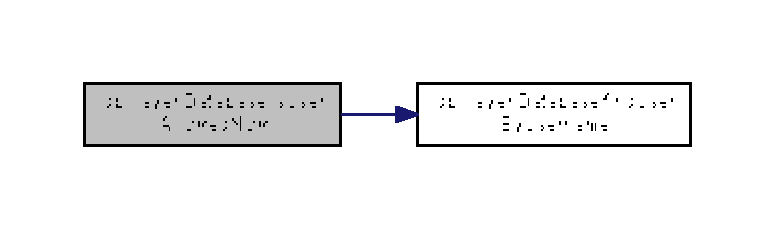
\includegraphics[width=350pt]{classdb__layer_1_1_database_af6ba4fcf6bcd589b0c85b05f49f46ef5_cgraph}
\end{center}
\end{figure}


\hypertarget{classdb__layer_1_1_database_a9ff75e8e93503e1e6b5ceb083910864a}{\index{db\-\_\-layer\-::\-Database@{db\-\_\-layer\-::\-Database}!is\-User\-Guest@{is\-User\-Guest}}
\index{is\-User\-Guest@{is\-User\-Guest}!db_layer::Database@{db\-\_\-layer\-::\-Database}}
\subsubsection[{is\-User\-Guest}]{\setlength{\rightskip}{0pt plus 5cm}def db\-\_\-layer.\-Database.\-is\-User\-Guest (
\begin{DoxyParamCaption}
\item[{}]{self, }
\item[{}]{username}
\end{DoxyParamCaption}
)}}\label{classdb__layer_1_1_database_a9ff75e8e93503e1e6b5ceb083910864a}


Definición en la línea 691 del archivo db\-\_\-layer.\-py.



Gráfico de llamadas para esta función\-:\nopagebreak
\begin{figure}[H]
\begin{center}
\leavevmode
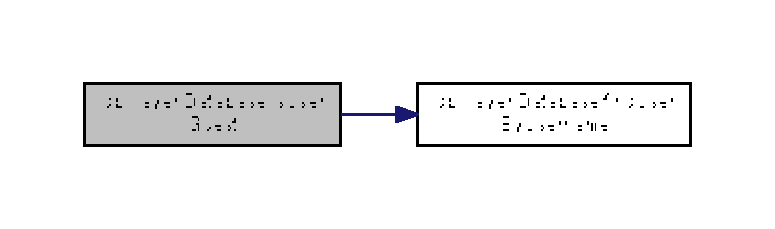
\includegraphics[width=350pt]{classdb__layer_1_1_database_a9ff75e8e93503e1e6b5ceb083910864a_cgraph}
\end{center}
\end{figure}


\hypertarget{classdb__layer_1_1_database_a3aaf3d095b7c6d005ec9061f83ccdc66}{\index{db\-\_\-layer\-::\-Database@{db\-\_\-layer\-::\-Database}!is\-User\-Kid@{is\-User\-Kid}}
\index{is\-User\-Kid@{is\-User\-Kid}!db_layer::Database@{db\-\_\-layer\-::\-Database}}
\subsubsection[{is\-User\-Kid}]{\setlength{\rightskip}{0pt plus 5cm}def db\-\_\-layer.\-Database.\-is\-User\-Kid (
\begin{DoxyParamCaption}
\item[{}]{self, }
\item[{}]{username}
\end{DoxyParamCaption}
)}}\label{classdb__layer_1_1_database_a3aaf3d095b7c6d005ec9061f83ccdc66}


Definición en la línea 679 del archivo db\-\_\-layer.\-py.



Gráfico de llamadas para esta función\-:\nopagebreak
\begin{figure}[H]
\begin{center}
\leavevmode
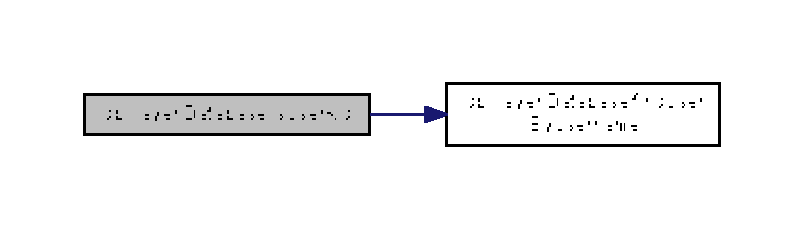
\includegraphics[width=350pt]{classdb__layer_1_1_database_a3aaf3d095b7c6d005ec9061f83ccdc66_cgraph}
\end{center}
\end{figure}


\hypertarget{classdb__layer_1_1_database_a03795c597d3a3ca0ef5d7c73299f8421}{\index{db\-\_\-layer\-::\-Database@{db\-\_\-layer\-::\-Database}!set\-User\-Admin@{set\-User\-Admin}}
\index{set\-User\-Admin@{set\-User\-Admin}!db_layer::Database@{db\-\_\-layer\-::\-Database}}
\subsubsection[{set\-User\-Admin}]{\setlength{\rightskip}{0pt plus 5cm}def db\-\_\-layer.\-Database.\-set\-User\-Admin (
\begin{DoxyParamCaption}
\item[{}]{self, }
\item[{}]{requested\-User}
\end{DoxyParamCaption}
)}}\label{classdb__layer_1_1_database_a03795c597d3a3ca0ef5d7c73299f8421}


Definición en la línea 332 del archivo db\-\_\-layer.\-py.



Gráfico de llamadas para esta función\-:\nopagebreak
\begin{figure}[H]
\begin{center}
\leavevmode
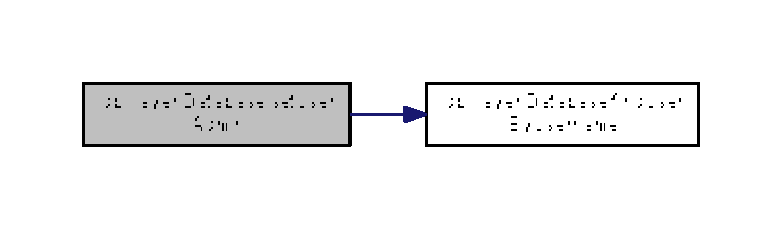
\includegraphics[width=350pt]{classdb__layer_1_1_database_a03795c597d3a3ca0ef5d7c73299f8421_cgraph}
\end{center}
\end{figure}


\hypertarget{classdb__layer_1_1_database_a203864bb4a53dfb89f57c23392559b46}{\index{db\-\_\-layer\-::\-Database@{db\-\_\-layer\-::\-Database}!set\-User\-Advanced@{set\-User\-Advanced}}
\index{set\-User\-Advanced@{set\-User\-Advanced}!db_layer::Database@{db\-\_\-layer\-::\-Database}}
\subsubsection[{set\-User\-Advanced}]{\setlength{\rightskip}{0pt plus 5cm}def db\-\_\-layer.\-Database.\-set\-User\-Advanced (
\begin{DoxyParamCaption}
\item[{}]{self, }
\item[{}]{requested\-User}
\end{DoxyParamCaption}
)}}\label{classdb__layer_1_1_database_a203864bb4a53dfb89f57c23392559b46}


Definición en la línea 375 del archivo db\-\_\-layer.\-py.



Gráfico de llamadas para esta función\-:\nopagebreak
\begin{figure}[H]
\begin{center}
\leavevmode
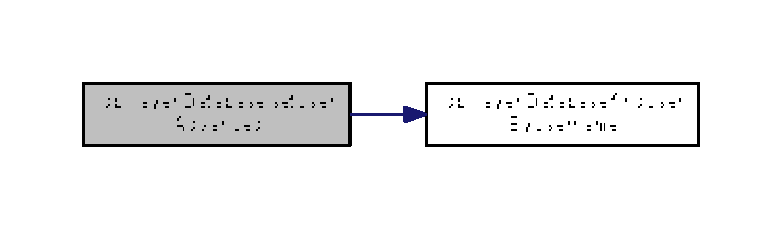
\includegraphics[width=350pt]{classdb__layer_1_1_database_a203864bb4a53dfb89f57c23392559b46_cgraph}
\end{center}
\end{figure}


\hypertarget{classdb__layer_1_1_database_ab86b18a8ab851b48703101ab53af6f8b}{\index{db\-\_\-layer\-::\-Database@{db\-\_\-layer\-::\-Database}!set\-User\-Guest@{set\-User\-Guest}}
\index{set\-User\-Guest@{set\-User\-Guest}!db_layer::Database@{db\-\_\-layer\-::\-Database}}
\subsubsection[{set\-User\-Guest}]{\setlength{\rightskip}{0pt plus 5cm}def db\-\_\-layer.\-Database.\-set\-User\-Guest (
\begin{DoxyParamCaption}
\item[{}]{self, }
\item[{}]{requested\-User}
\end{DoxyParamCaption}
)}}\label{classdb__layer_1_1_database_ab86b18a8ab851b48703101ab53af6f8b}


Definición en la línea 407 del archivo db\-\_\-layer.\-py.



Gráfico de llamadas para esta función\-:\nopagebreak
\begin{figure}[H]
\begin{center}
\leavevmode
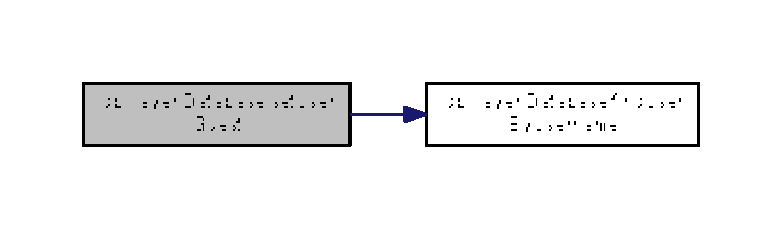
\includegraphics[width=350pt]{classdb__layer_1_1_database_ab86b18a8ab851b48703101ab53af6f8b_cgraph}
\end{center}
\end{figure}


\hypertarget{classdb__layer_1_1_database_a03a583931163ed9bac45c5b05e4bf69f}{\index{db\-\_\-layer\-::\-Database@{db\-\_\-layer\-::\-Database}!set\-User\-Kid@{set\-User\-Kid}}
\index{set\-User\-Kid@{set\-User\-Kid}!db_layer::Database@{db\-\_\-layer\-::\-Database}}
\subsubsection[{set\-User\-Kid}]{\setlength{\rightskip}{0pt plus 5cm}def db\-\_\-layer.\-Database.\-set\-User\-Kid (
\begin{DoxyParamCaption}
\item[{}]{self, }
\item[{}]{requested\-User}
\end{DoxyParamCaption}
)}}\label{classdb__layer_1_1_database_a03a583931163ed9bac45c5b05e4bf69f}


Definición en la línea 391 del archivo db\-\_\-layer.\-py.



Gráfico de llamadas para esta función\-:\nopagebreak
\begin{figure}[H]
\begin{center}
\leavevmode
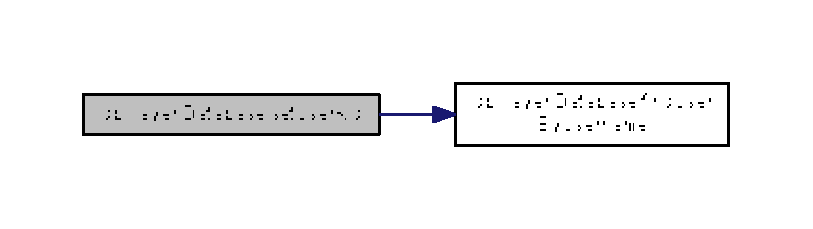
\includegraphics[width=350pt]{classdb__layer_1_1_database_a03a583931163ed9bac45c5b05e4bf69f_cgraph}
\end{center}
\end{figure}


\hypertarget{classdb__layer_1_1_database_aa682552b52caba32fde23ef44fb63ade}{\index{db\-\_\-layer\-::\-Database@{db\-\_\-layer\-::\-Database}!wr\-\_\-add\-Relation@{wr\-\_\-add\-Relation}}
\index{wr\-\_\-add\-Relation@{wr\-\_\-add\-Relation}!db_layer::Database@{db\-\_\-layer\-::\-Database}}
\subsubsection[{wr\-\_\-add\-Relation}]{\setlength{\rightskip}{0pt plus 5cm}def db\-\_\-layer.\-Database.\-wr\-\_\-add\-Relation (
\begin{DoxyParamCaption}
\item[{}]{self, }
\item[{}]{the\-Dict}
\end{DoxyParamCaption}
)}}\label{classdb__layer_1_1_database_aa682552b52caba32fde23ef44fb63ade}


Definición en la línea 279 del archivo db\-\_\-layer.\-py.



Gráfico de llamadas para esta función\-:\nopagebreak
\begin{figure}[H]
\begin{center}
\leavevmode
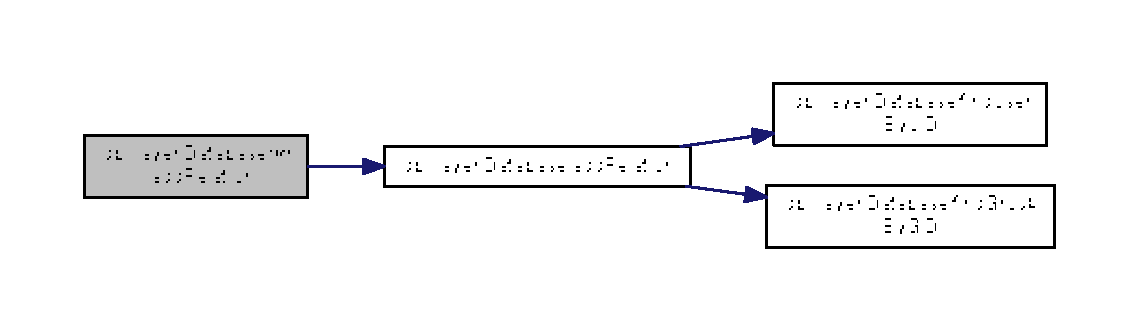
\includegraphics[width=350pt]{classdb__layer_1_1_database_aa682552b52caba32fde23ef44fb63ade_cgraph}
\end{center}
\end{figure}


\hypertarget{classdb__layer_1_1_database_ab20da0ac6137c6a276f27f59a90d87e3}{\index{db\-\_\-layer\-::\-Database@{db\-\_\-layer\-::\-Database}!wr\-\_\-del\-Relation@{wr\-\_\-del\-Relation}}
\index{wr\-\_\-del\-Relation@{wr\-\_\-del\-Relation}!db_layer::Database@{db\-\_\-layer\-::\-Database}}
\subsubsection[{wr\-\_\-del\-Relation}]{\setlength{\rightskip}{0pt plus 5cm}def db\-\_\-layer.\-Database.\-wr\-\_\-del\-Relation (
\begin{DoxyParamCaption}
\item[{}]{self, }
\item[{}]{the\-Dict}
\end{DoxyParamCaption}
)}}\label{classdb__layer_1_1_database_ab20da0ac6137c6a276f27f59a90d87e3}


Definición en la línea 299 del archivo db\-\_\-layer.\-py.



Gráfico de llamadas para esta función\-:\nopagebreak
\begin{figure}[H]
\begin{center}
\leavevmode
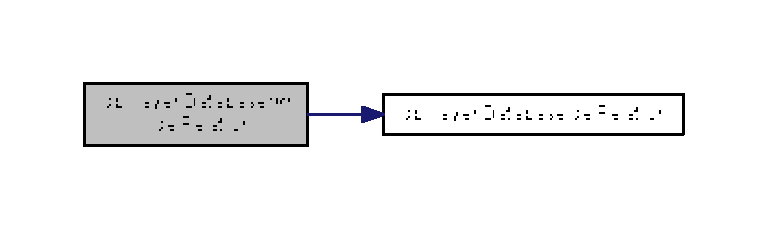
\includegraphics[width=350pt]{classdb__layer_1_1_database_ab20da0ac6137c6a276f27f59a90d87e3_cgraph}
\end{center}
\end{figure}


\hypertarget{classdb__layer_1_1_database_ac2a8936466701acf8972dd1dbb73d0ad}{\index{db\-\_\-layer\-::\-Database@{db\-\_\-layer\-::\-Database}!wr\-\_\-insert\-M\-I\-M\-E\-Sby\-G\-I\-D@{wr\-\_\-insert\-M\-I\-M\-E\-Sby\-G\-I\-D}}
\index{wr\-\_\-insert\-M\-I\-M\-E\-Sby\-G\-I\-D@{wr\-\_\-insert\-M\-I\-M\-E\-Sby\-G\-I\-D}!db_layer::Database@{db\-\_\-layer\-::\-Database}}
\subsubsection[{wr\-\_\-insert\-M\-I\-M\-E\-Sby\-G\-I\-D}]{\setlength{\rightskip}{0pt plus 5cm}def db\-\_\-layer.\-Database.\-wr\-\_\-insert\-M\-I\-M\-E\-Sby\-G\-I\-D (
\begin{DoxyParamCaption}
\item[{}]{self, }
\item[{}]{the\-Dict}
\end{DoxyParamCaption}
)}}\label{classdb__layer_1_1_database_ac2a8936466701acf8972dd1dbb73d0ad}


Definición en la línea 881 del archivo db\-\_\-layer.\-py.



Gráfico de llamadas para esta función\-:\nopagebreak
\begin{figure}[H]
\begin{center}
\leavevmode
\includegraphics[width=350pt]{classdb__layer_1_1_database_ac2a8936466701acf8972dd1dbb73d0ad_cgraph}
\end{center}
\end{figure}


\hypertarget{classdb__layer_1_1_database_a3ede692ddfa18fd73ce142341f21e6a0}{\index{db\-\_\-layer\-::\-Database@{db\-\_\-layer\-::\-Database}!wr\-\_\-insert\-U\-R\-I\-Sby\-G\-I\-D@{wr\-\_\-insert\-U\-R\-I\-Sby\-G\-I\-D}}
\index{wr\-\_\-insert\-U\-R\-I\-Sby\-G\-I\-D@{wr\-\_\-insert\-U\-R\-I\-Sby\-G\-I\-D}!db_layer::Database@{db\-\_\-layer\-::\-Database}}
\subsubsection[{wr\-\_\-insert\-U\-R\-I\-Sby\-G\-I\-D}]{\setlength{\rightskip}{0pt plus 5cm}def db\-\_\-layer.\-Database.\-wr\-\_\-insert\-U\-R\-I\-Sby\-G\-I\-D (
\begin{DoxyParamCaption}
\item[{}]{self, }
\item[{}]{the\-Dict}
\end{DoxyParamCaption}
)}}\label{classdb__layer_1_1_database_a3ede692ddfa18fd73ce142341f21e6a0}


Definición en la línea 790 del archivo db\-\_\-layer.\-py.



Gráfico de llamadas para esta función\-:\nopagebreak
\begin{figure}[H]
\begin{center}
\leavevmode
\includegraphics[width=350pt]{classdb__layer_1_1_database_a3ede692ddfa18fd73ce142341f21e6a0_cgraph}
\end{center}
\end{figure}


\hypertarget{classdb__layer_1_1_database_abf6ce37aea5202f161dbd3e3c41d6a6e}{\index{db\-\_\-layer\-::\-Database@{db\-\_\-layer\-::\-Database}!wr\-\_\-insert\-W\-O\-R\-D\-Sby\-G\-I\-D@{wr\-\_\-insert\-W\-O\-R\-D\-Sby\-G\-I\-D}}
\index{wr\-\_\-insert\-W\-O\-R\-D\-Sby\-G\-I\-D@{wr\-\_\-insert\-W\-O\-R\-D\-Sby\-G\-I\-D}!db_layer::Database@{db\-\_\-layer\-::\-Database}}
\subsubsection[{wr\-\_\-insert\-W\-O\-R\-D\-Sby\-G\-I\-D}]{\setlength{\rightskip}{0pt plus 5cm}def db\-\_\-layer.\-Database.\-wr\-\_\-insert\-W\-O\-R\-D\-Sby\-G\-I\-D (
\begin{DoxyParamCaption}
\item[{}]{self, }
\item[{}]{the\-Dict}
\end{DoxyParamCaption}
)}}\label{classdb__layer_1_1_database_abf6ce37aea5202f161dbd3e3c41d6a6e}


Definición en la línea 836 del archivo db\-\_\-layer.\-py.



Gráfico de llamadas para esta función\-:\nopagebreak
\begin{figure}[H]
\begin{center}
\leavevmode
\includegraphics[width=350pt]{classdb__layer_1_1_database_abf6ce37aea5202f161dbd3e3c41d6a6e_cgraph}
\end{center}
\end{figure}




\subsection{Documentación de los datos miembro}
\hypertarget{classdb__layer_1_1_database_a232d5477efc9b4c8d8a36b7541c851e1}{\index{db\-\_\-layer\-::\-Database@{db\-\_\-layer\-::\-Database}!session@{session}}
\index{session@{session}!db_layer::Database@{db\-\_\-layer\-::\-Database}}
\subsubsection[{session}]{\setlength{\rightskip}{0pt plus 5cm}db\-\_\-layer.\-Database.\-session = None\hspace{0.3cm}{\ttfamily [static]}}}\label{classdb__layer_1_1_database_a232d5477efc9b4c8d8a36b7541c851e1}


Definición en la línea 109 del archivo db\-\_\-layer.\-py.



La documentación para esta clase fue generada a partir del siguiente fichero\-:\begin{DoxyCompactItemize}
\item 
\hyperlink{db__layer_8py}{db\-\_\-layer.\-py}\end{DoxyCompactItemize}

\hypertarget{classdb__log_1_1_database}{\section{Referencia de la Clase db\-\_\-log.\-Database}
\label{classdb__log_1_1_database}\index{db\-\_\-log.\-Database@{db\-\_\-log.\-Database}}
}
\subsection*{Métodos públicos}
\begin{DoxyCompactItemize}
\item 
def \hyperlink{classdb__log_1_1_database_a8ca8cf39fcc9ed91f39d6a8254cd38ca}{\-\_\-\-\_\-init\-\_\-\-\_\-}
\item 
def \hyperlink{classdb__log_1_1_database_ae34e71223e9896b44ef7ad9e9426718b}{get\-Last\-Lines}
\item 
def \hyperlink{classdb__log_1_1_database_a395b1cf70a83f2d01422566d3e08484c}{add\-Line}
\end{DoxyCompactItemize}
\subsection*{Atributos públicos estáticos}
\begin{DoxyCompactItemize}
\item 
\hyperlink{classdb__log_1_1_database_af6b2deacd2e4d21f3292d2143a4e14ba}{session} = None
\end{DoxyCompactItemize}


\subsection{Descripción detallada}


Definición en la línea 31 del archivo db\-\_\-log.\-py.



\subsection{Documentación del constructor y destructor}
\hypertarget{classdb__log_1_1_database_a8ca8cf39fcc9ed91f39d6a8254cd38ca}{\index{db\-\_\-log\-::\-Database@{db\-\_\-log\-::\-Database}!\-\_\-\-\_\-init\-\_\-\-\_\-@{\-\_\-\-\_\-init\-\_\-\-\_\-}}
\index{\-\_\-\-\_\-init\-\_\-\-\_\-@{\-\_\-\-\_\-init\-\_\-\-\_\-}!db_log::Database@{db\-\_\-log\-::\-Database}}
\subsubsection[{\-\_\-\-\_\-init\-\_\-\-\_\-}]{\setlength{\rightskip}{0pt plus 5cm}def db\-\_\-log.\-Database.\-\_\-\-\_\-init\-\_\-\-\_\- (
\begin{DoxyParamCaption}
\item[{}]{self}
\end{DoxyParamCaption}
)}}\label{classdb__log_1_1_database_a8ca8cf39fcc9ed91f39d6a8254cd38ca}


Definición en la línea 37 del archivo db\-\_\-log.\-py.



\subsection{Documentación de las funciones miembro}
\hypertarget{classdb__log_1_1_database_a395b1cf70a83f2d01422566d3e08484c}{\index{db\-\_\-log\-::\-Database@{db\-\_\-log\-::\-Database}!add\-Line@{add\-Line}}
\index{add\-Line@{add\-Line}!db_log::Database@{db\-\_\-log\-::\-Database}}
\subsubsection[{add\-Line}]{\setlength{\rightskip}{0pt plus 5cm}def db\-\_\-log.\-Database.\-add\-Line (
\begin{DoxyParamCaption}
\item[{}]{self, }
\item[{}]{data}
\end{DoxyParamCaption}
)}}\label{classdb__log_1_1_database_a395b1cf70a83f2d01422566d3e08484c}


Definición en la línea 63 del archivo db\-\_\-log.\-py.

\hypertarget{classdb__log_1_1_database_ae34e71223e9896b44ef7ad9e9426718b}{\index{db\-\_\-log\-::\-Database@{db\-\_\-log\-::\-Database}!get\-Last\-Lines@{get\-Last\-Lines}}
\index{get\-Last\-Lines@{get\-Last\-Lines}!db_log::Database@{db\-\_\-log\-::\-Database}}
\subsubsection[{get\-Last\-Lines}]{\setlength{\rightskip}{0pt plus 5cm}def db\-\_\-log.\-Database.\-get\-Last\-Lines (
\begin{DoxyParamCaption}
\item[{}]{self, }
\item[{}]{num\-Lines}
\end{DoxyParamCaption}
)}}\label{classdb__log_1_1_database_ae34e71223e9896b44ef7ad9e9426718b}


Definición en la línea 53 del archivo db\-\_\-log.\-py.



\subsection{Documentación de los datos miembro}
\hypertarget{classdb__log_1_1_database_af6b2deacd2e4d21f3292d2143a4e14ba}{\index{db\-\_\-log\-::\-Database@{db\-\_\-log\-::\-Database}!session@{session}}
\index{session@{session}!db_log::Database@{db\-\_\-log\-::\-Database}}
\subsubsection[{session}]{\setlength{\rightskip}{0pt plus 5cm}db\-\_\-log.\-Database.\-session = None\hspace{0.3cm}{\ttfamily [static]}}}\label{classdb__log_1_1_database_af6b2deacd2e4d21f3292d2143a4e14ba}


Definición en la línea 36 del archivo db\-\_\-log.\-py.



La documentación para esta clase fue generada a partir del siguiente fichero\-:\begin{DoxyCompactItemize}
\item 
\hyperlink{db__log_8py}{db\-\_\-log.\-py}\end{DoxyCompactItemize}

\hypertarget{classdb__mapper_1_1db__handler}{\section{Referencia de la Clase db\-\_\-mapper.\-db\-\_\-handler}
\label{classdb__mapper_1_1db__handler}\index{db\-\_\-mapper.\-db\-\_\-handler@{db\-\_\-mapper.\-db\-\_\-handler}}
}
\subsection*{Métodos públicos}
\begin{DoxyCompactItemize}
\item 
def \hyperlink{classdb__mapper_1_1db__handler_a479a5e4baa7d3a4a0c086b5f20b19886}{\-\_\-\-\_\-init\-\_\-\-\_\-}
\item 
def \hyperlink{classdb__mapper_1_1db__handler_a5fcc6f04805b1668cfdd37a56b96e481}{answer\-\_\-wrapper}
\item 
def \hyperlink{classdb__mapper_1_1db__handler_a4d3b0376c65e8fafd85e7ebd66c9b268}{map\-\_\-db2answer}
\item 
def \hyperlink{classdb__mapper_1_1db__handler_adebfe1a956d4058883ce07bdaf253365}{handle\-\_\-request}
\item 
def \hyperlink{classdb__mapper_1_1db__handler_acab02d962db6d8b42cdeae79bf46425d}{map\-\_\-query2db}
\item 
def \hyperlink{classdb__mapper_1_1db__handler_ab82596ecdbec3136052c2f63ea282f0c}{map\-\_\-parms2db}
\item 
def \hyperlink{classdb__mapper_1_1db__handler_aadb435084c4d5fccc96513605042b49b}{map\-\_\-dict2\-User}
\item 
def \hyperlink{classdb__mapper_1_1db__handler_aa0a226e11a8afd0b8dfa20fd76362832}{map\-\_\-dict2\-Group}
\item 
def \hyperlink{classdb__mapper_1_1db__handler_a7f56361e908c36b3b9a89679276b70c9}{map\-\_\-dict2\-U\-R\-I\-S}
\item 
def \hyperlink{classdb__mapper_1_1db__handler_a622709833c8db8cf253628fb6e599f17}{map\-\_\-dict2\-W\-O\-R\-D\-S}
\item 
def \hyperlink{classdb__mapper_1_1db__handler_a911bd297d667fd50426a75ad13ab8779}{map\-\_\-dict2\-M\-I\-M\-E\-S}
\end{DoxyCompactItemize}


\subsection{Descripción detallada}


Definición en la línea 17 del archivo db\-\_\-mapper.\-py.



\subsection{Documentación del constructor y destructor}
\hypertarget{classdb__mapper_1_1db__handler_a479a5e4baa7d3a4a0c086b5f20b19886}{\index{db\-\_\-mapper\-::db\-\_\-handler@{db\-\_\-mapper\-::db\-\_\-handler}!\-\_\-\-\_\-init\-\_\-\-\_\-@{\-\_\-\-\_\-init\-\_\-\-\_\-}}
\index{\-\_\-\-\_\-init\-\_\-\-\_\-@{\-\_\-\-\_\-init\-\_\-\-\_\-}!db_mapper::db_handler@{db\-\_\-mapper\-::db\-\_\-handler}}
\subsubsection[{\-\_\-\-\_\-init\-\_\-\-\_\-}]{\setlength{\rightskip}{0pt plus 5cm}def db\-\_\-mapper.\-db\-\_\-handler.\-\_\-\-\_\-init\-\_\-\-\_\- (
\begin{DoxyParamCaption}
\item[{}]{self}
\end{DoxyParamCaption}
)}}\label{classdb__mapper_1_1db__handler_a479a5e4baa7d3a4a0c086b5f20b19886}


Definición en la línea 21 del archivo db\-\_\-mapper.\-py.



\subsection{Documentación de las funciones miembro}
\hypertarget{classdb__mapper_1_1db__handler_a5fcc6f04805b1668cfdd37a56b96e481}{\index{db\-\_\-mapper\-::db\-\_\-handler@{db\-\_\-mapper\-::db\-\_\-handler}!answer\-\_\-wrapper@{answer\-\_\-wrapper}}
\index{answer\-\_\-wrapper@{answer\-\_\-wrapper}!db_mapper::db_handler@{db\-\_\-mapper\-::db\-\_\-handler}}
\subsubsection[{answer\-\_\-wrapper}]{\setlength{\rightskip}{0pt plus 5cm}def db\-\_\-mapper.\-db\-\_\-handler.\-answer\-\_\-wrapper (
\begin{DoxyParamCaption}
\item[{}]{self, }
\item[{}]{to\-\_\-type, }
\item[{}]{answer}
\end{DoxyParamCaption}
)}}\label{classdb__mapper_1_1db__handler_a5fcc6f04805b1668cfdd37a56b96e481}


Definición en la línea 25 del archivo db\-\_\-mapper.\-py.



Gráfico de llamadas a esta función\-:\nopagebreak
\begin{figure}[H]
\begin{center}
\leavevmode
\includegraphics[width=350pt]{classdb__mapper_1_1db__handler_a5fcc6f04805b1668cfdd37a56b96e481_icgraph}
\end{center}
\end{figure}


\hypertarget{classdb__mapper_1_1db__handler_adebfe1a956d4058883ce07bdaf253365}{\index{db\-\_\-mapper\-::db\-\_\-handler@{db\-\_\-mapper\-::db\-\_\-handler}!handle\-\_\-request@{handle\-\_\-request}}
\index{handle\-\_\-request@{handle\-\_\-request}!db_mapper::db_handler@{db\-\_\-mapper\-::db\-\_\-handler}}
\subsubsection[{handle\-\_\-request}]{\setlength{\rightskip}{0pt plus 5cm}def db\-\_\-mapper.\-db\-\_\-handler.\-handle\-\_\-request (
\begin{DoxyParamCaption}
\item[{}]{self, }
\item[{}]{query, }
\item[{}]{parms}
\end{DoxyParamCaption}
)}}\label{classdb__mapper_1_1db__handler_adebfe1a956d4058883ce07bdaf253365}


Definición en la línea 53 del archivo db\-\_\-mapper.\-py.



Gráfico de llamadas para esta función\-:\nopagebreak
\begin{figure}[H]
\begin{center}
\leavevmode
\includegraphics[width=350pt]{classdb__mapper_1_1db__handler_adebfe1a956d4058883ce07bdaf253365_cgraph}
\end{center}
\end{figure}


\hypertarget{classdb__mapper_1_1db__handler_a4d3b0376c65e8fafd85e7ebd66c9b268}{\index{db\-\_\-mapper\-::db\-\_\-handler@{db\-\_\-mapper\-::db\-\_\-handler}!map\-\_\-db2answer@{map\-\_\-db2answer}}
\index{map\-\_\-db2answer@{map\-\_\-db2answer}!db_mapper::db_handler@{db\-\_\-mapper\-::db\-\_\-handler}}
\subsubsection[{map\-\_\-db2answer}]{\setlength{\rightskip}{0pt plus 5cm}def db\-\_\-mapper.\-db\-\_\-handler.\-map\-\_\-db2answer (
\begin{DoxyParamCaption}
\item[{}]{self, }
\item[{}]{query, }
\item[{}]{answer}
\end{DoxyParamCaption}
)}}\label{classdb__mapper_1_1db__handler_a4d3b0376c65e8fafd85e7ebd66c9b268}


Definición en la línea 41 del archivo db\-\_\-mapper.\-py.



Gráfico de llamadas para esta función\-:\nopagebreak
\begin{figure}[H]
\begin{center}
\leavevmode
\includegraphics[width=350pt]{classdb__mapper_1_1db__handler_a4d3b0376c65e8fafd85e7ebd66c9b268_cgraph}
\end{center}
\end{figure}




Gráfico de llamadas a esta función\-:\nopagebreak
\begin{figure}[H]
\begin{center}
\leavevmode
\includegraphics[width=350pt]{classdb__mapper_1_1db__handler_a4d3b0376c65e8fafd85e7ebd66c9b268_icgraph}
\end{center}
\end{figure}


\hypertarget{classdb__mapper_1_1db__handler_aa0a226e11a8afd0b8dfa20fd76362832}{\index{db\-\_\-mapper\-::db\-\_\-handler@{db\-\_\-mapper\-::db\-\_\-handler}!map\-\_\-dict2\-Group@{map\-\_\-dict2\-Group}}
\index{map\-\_\-dict2\-Group@{map\-\_\-dict2\-Group}!db_mapper::db_handler@{db\-\_\-mapper\-::db\-\_\-handler}}
\subsubsection[{map\-\_\-dict2\-Group}]{\setlength{\rightskip}{0pt plus 5cm}def db\-\_\-mapper.\-db\-\_\-handler.\-map\-\_\-dict2\-Group (
\begin{DoxyParamCaption}
\item[{}]{self, }
\item[{}]{parms}
\end{DoxyParamCaption}
)}}\label{classdb__mapper_1_1db__handler_aa0a226e11a8afd0b8dfa20fd76362832}


Definición en la línea 151 del archivo db\-\_\-mapper.\-py.



Gráfico de llamadas a esta función\-:\nopagebreak
\begin{figure}[H]
\begin{center}
\leavevmode
\includegraphics[width=350pt]{classdb__mapper_1_1db__handler_aa0a226e11a8afd0b8dfa20fd76362832_icgraph}
\end{center}
\end{figure}


\hypertarget{classdb__mapper_1_1db__handler_a911bd297d667fd50426a75ad13ab8779}{\index{db\-\_\-mapper\-::db\-\_\-handler@{db\-\_\-mapper\-::db\-\_\-handler}!map\-\_\-dict2\-M\-I\-M\-E\-S@{map\-\_\-dict2\-M\-I\-M\-E\-S}}
\index{map\-\_\-dict2\-M\-I\-M\-E\-S@{map\-\_\-dict2\-M\-I\-M\-E\-S}!db_mapper::db_handler@{db\-\_\-mapper\-::db\-\_\-handler}}
\subsubsection[{map\-\_\-dict2\-M\-I\-M\-E\-S}]{\setlength{\rightskip}{0pt plus 5cm}def db\-\_\-mapper.\-db\-\_\-handler.\-map\-\_\-dict2\-M\-I\-M\-E\-S (
\begin{DoxyParamCaption}
\item[{}]{self, }
\item[{}]{parms}
\end{DoxyParamCaption}
)}}\label{classdb__mapper_1_1db__handler_a911bd297d667fd50426a75ad13ab8779}


Definición en la línea 204 del archivo db\-\_\-mapper.\-py.

\hypertarget{classdb__mapper_1_1db__handler_a7f56361e908c36b3b9a89679276b70c9}{\index{db\-\_\-mapper\-::db\-\_\-handler@{db\-\_\-mapper\-::db\-\_\-handler}!map\-\_\-dict2\-U\-R\-I\-S@{map\-\_\-dict2\-U\-R\-I\-S}}
\index{map\-\_\-dict2\-U\-R\-I\-S@{map\-\_\-dict2\-U\-R\-I\-S}!db_mapper::db_handler@{db\-\_\-mapper\-::db\-\_\-handler}}
\subsubsection[{map\-\_\-dict2\-U\-R\-I\-S}]{\setlength{\rightskip}{0pt plus 5cm}def db\-\_\-mapper.\-db\-\_\-handler.\-map\-\_\-dict2\-U\-R\-I\-S (
\begin{DoxyParamCaption}
\item[{}]{self, }
\item[{}]{parms}
\end{DoxyParamCaption}
)}}\label{classdb__mapper_1_1db__handler_a7f56361e908c36b3b9a89679276b70c9}


Definición en la línea 168 del archivo db\-\_\-mapper.\-py.

\hypertarget{classdb__mapper_1_1db__handler_aadb435084c4d5fccc96513605042b49b}{\index{db\-\_\-mapper\-::db\-\_\-handler@{db\-\_\-mapper\-::db\-\_\-handler}!map\-\_\-dict2\-User@{map\-\_\-dict2\-User}}
\index{map\-\_\-dict2\-User@{map\-\_\-dict2\-User}!db_mapper::db_handler@{db\-\_\-mapper\-::db\-\_\-handler}}
\subsubsection[{map\-\_\-dict2\-User}]{\setlength{\rightskip}{0pt plus 5cm}def db\-\_\-mapper.\-db\-\_\-handler.\-map\-\_\-dict2\-User (
\begin{DoxyParamCaption}
\item[{}]{self, }
\item[{}]{parms}
\end{DoxyParamCaption}
)}}\label{classdb__mapper_1_1db__handler_aadb435084c4d5fccc96513605042b49b}


Definición en la línea 134 del archivo db\-\_\-mapper.\-py.



Gráfico de llamadas a esta función\-:\nopagebreak
\begin{figure}[H]
\begin{center}
\leavevmode
\includegraphics[width=350pt]{classdb__mapper_1_1db__handler_aadb435084c4d5fccc96513605042b49b_icgraph}
\end{center}
\end{figure}


\hypertarget{classdb__mapper_1_1db__handler_a622709833c8db8cf253628fb6e599f17}{\index{db\-\_\-mapper\-::db\-\_\-handler@{db\-\_\-mapper\-::db\-\_\-handler}!map\-\_\-dict2\-W\-O\-R\-D\-S@{map\-\_\-dict2\-W\-O\-R\-D\-S}}
\index{map\-\_\-dict2\-W\-O\-R\-D\-S@{map\-\_\-dict2\-W\-O\-R\-D\-S}!db_mapper::db_handler@{db\-\_\-mapper\-::db\-\_\-handler}}
\subsubsection[{map\-\_\-dict2\-W\-O\-R\-D\-S}]{\setlength{\rightskip}{0pt plus 5cm}def db\-\_\-mapper.\-db\-\_\-handler.\-map\-\_\-dict2\-W\-O\-R\-D\-S (
\begin{DoxyParamCaption}
\item[{}]{self, }
\item[{}]{parms}
\end{DoxyParamCaption}
)}}\label{classdb__mapper_1_1db__handler_a622709833c8db8cf253628fb6e599f17}


Definición en la línea 187 del archivo db\-\_\-mapper.\-py.

\hypertarget{classdb__mapper_1_1db__handler_ab82596ecdbec3136052c2f63ea282f0c}{\index{db\-\_\-mapper\-::db\-\_\-handler@{db\-\_\-mapper\-::db\-\_\-handler}!map\-\_\-parms2db@{map\-\_\-parms2db}}
\index{map\-\_\-parms2db@{map\-\_\-parms2db}!db_mapper::db_handler@{db\-\_\-mapper\-::db\-\_\-handler}}
\subsubsection[{map\-\_\-parms2db}]{\setlength{\rightskip}{0pt plus 5cm}def db\-\_\-mapper.\-db\-\_\-handler.\-map\-\_\-parms2db (
\begin{DoxyParamCaption}
\item[{}]{self, }
\item[{}]{query, }
\item[{}]{parms}
\end{DoxyParamCaption}
)}}\label{classdb__mapper_1_1db__handler_ab82596ecdbec3136052c2f63ea282f0c}


Definición en la línea 105 del archivo db\-\_\-mapper.\-py.



Gráfico de llamadas para esta función\-:\nopagebreak
\begin{figure}[H]
\begin{center}
\leavevmode
\includegraphics[width=350pt]{classdb__mapper_1_1db__handler_ab82596ecdbec3136052c2f63ea282f0c_cgraph}
\end{center}
\end{figure}




Gráfico de llamadas a esta función\-:\nopagebreak
\begin{figure}[H]
\begin{center}
\leavevmode
\includegraphics[width=350pt]{classdb__mapper_1_1db__handler_ab82596ecdbec3136052c2f63ea282f0c_icgraph}
\end{center}
\end{figure}


\hypertarget{classdb__mapper_1_1db__handler_acab02d962db6d8b42cdeae79bf46425d}{\index{db\-\_\-mapper\-::db\-\_\-handler@{db\-\_\-mapper\-::db\-\_\-handler}!map\-\_\-query2db@{map\-\_\-query2db}}
\index{map\-\_\-query2db@{map\-\_\-query2db}!db_mapper::db_handler@{db\-\_\-mapper\-::db\-\_\-handler}}
\subsubsection[{map\-\_\-query2db}]{\setlength{\rightskip}{0pt plus 5cm}def db\-\_\-mapper.\-db\-\_\-handler.\-map\-\_\-query2db (
\begin{DoxyParamCaption}
\item[{}]{self, }
\item[{}]{query}
\end{DoxyParamCaption}
)}}\label{classdb__mapper_1_1db__handler_acab02d962db6d8b42cdeae79bf46425d}


Definición en la línea 72 del archivo db\-\_\-mapper.\-py.



Gráfico de llamadas a esta función\-:\nopagebreak
\begin{figure}[H]
\begin{center}
\leavevmode
\includegraphics[width=350pt]{classdb__mapper_1_1db__handler_acab02d962db6d8b42cdeae79bf46425d_icgraph}
\end{center}
\end{figure}




La documentación para esta clase fue generada a partir del siguiente fichero\-:\begin{DoxyCompactItemize}
\item 
\hyperlink{db__mapper_8py}{db\-\_\-mapper.\-py}\end{DoxyCompactItemize}

\hypertarget{class_cache_1_1_file_cache}{\section{Referencia de la Clase Cache.\-File\-Cache}
\label{class_cache_1_1_file_cache}\index{Cache.\-File\-Cache@{Cache.\-File\-Cache}}
}


Diagrama de colaboración para Cache.\-File\-Cache\-:\nopagebreak
\begin{figure}[H]
\begin{center}
\leavevmode
\includegraphics[width=226pt]{class_cache_1_1_file_cache__coll__graph}
\end{center}
\end{figure}
\subsection*{Métodos públicos}
\begin{DoxyCompactItemize}
\item 
def \hyperlink{class_cache_1_1_file_cache_ac5fa19d6e9b990f58ae6969abfdeceed}{remove\-\_\-html\-\_\-markup}
\item 
def \hyperlink{class_cache_1_1_file_cache_a794781e8000f88b6990d1d1a2b24fbe6}{\-\_\-\-\_\-init\-\_\-\-\_\-}
\item 
def \hyperlink{class_cache_1_1_file_cache_a3a0ff0a693d8eb05c5635ac68c86a65b}{setup}
\item 
def \hyperlink{class_cache_1_1_file_cache_a45b17bfd8c65aa650fd0f53209d03b5c}{is\-\_\-cached}
\item 
def \hyperlink{class_cache_1_1_file_cache_a474cd0cce36603d869add65a52ec852b}{put}
\item 
def \hyperlink{class_cache_1_1_file_cache_a6580598cf60ffda8176dbe4036c4929c}{get}
\end{DoxyCompactItemize}
\subsection*{Atributos públicos}
\begin{DoxyCompactItemize}
\item 
\hyperlink{class_cache_1_1_file_cache_ac795fe342f956e8b8cd2ec23267c674d}{was\-\_\-checked}
\item 
\hyperlink{class_cache_1_1_file_cache_aca5f594f2c828bbb00e29385b527b5c4}{D\-E\-B\-U\-G}
\item 
\hyperlink{class_cache_1_1_file_cache_a969a9af6b255a6d9b14d71ee429cf6af}{path}
\item 
\hyperlink{class_cache_1_1_file_cache_a2b1c48cd0ee88344f405391545633787}{md5hash}
\item 
\hyperlink{class_cache_1_1_file_cache_ad4c782bcbd654eff2aea4c3b76815723}{cache\-\_\-filename\-\_\-base}
\item 
\hyperlink{class_cache_1_1_file_cache_abb789c23d266d9148f2fb9c3bc3e8d3c}{cache\-\_\-filename\-\_\-meta}
\item 
\hyperlink{class_cache_1_1_file_cache_af64994359a6b953e12a1f3352cbf057a}{cache\-\_\-filename\-\_\-cache}
\item 
\hyperlink{class_cache_1_1_file_cache_a4a427efcf91e7550463882b99d6b3df2}{cache\-\_\-filename\-\_\-header}
\item 
\hyperlink{class_cache_1_1_file_cache_a7a879f97bdb8d6f8a5b14390db395cdf}{cache\-\_\-filename\-\_\-strip}
\item 
\hyperlink{class_cache_1_1_file_cache_a6660cc5f8e2408bdece63291305a5e5e}{content\-\_\-stripped}
\end{DoxyCompactItemize}
\subsection*{Atributos públicos estáticos}
\begin{DoxyCompactItemize}
\item 
string \hyperlink{class_cache_1_1_file_cache_aa3e48c8aceb54811558590d05769af11}{path} = ''
\item 
string \hyperlink{class_cache_1_1_file_cache_a94712bab05ce67c5a20c3e2cfba47509}{md5hash\-\_\-str} = ''
\item 
string \hyperlink{class_cache_1_1_file_cache_a643dfb38067e5c4785397ef0e8c20944}{cache\-\_\-filename\-\_\-base} = ''
\item 
string \hyperlink{class_cache_1_1_file_cache_ab6e30d3196eea1c3cae1186945c8e0e2}{cache\-\_\-filename\-\_\-meta} = ''
\item 
string \hyperlink{class_cache_1_1_file_cache_abf7b20e99585e8ff1fd1c205eb02c2b3}{cache\-\_\-filename\-\_\-cache} = ''
\item 
string \hyperlink{class_cache_1_1_file_cache_a2f7d1283375128a83f657d9eb2ed5d3d}{cache\-\_\-filename\-\_\-strip} = ''
\item 
string \hyperlink{class_cache_1_1_file_cache_a27cec37d2b4d4aac26eb0999e220031e}{cache\-\_\-filename\-\_\-header} = ''
\item 
\hyperlink{class_cache_1_1_file_cache_afda3d5760616e47bd8fda4fe7490d7a9}{content\-\_\-is\-\_\-text} = False
\item 
tuple \hyperlink{class_cache_1_1_file_cache_a6add3c86ea9523a23c289b660d064e57}{content\-\_\-stripped} = bytes()
\item 
tuple \hyperlink{class_cache_1_1_file_cache_a7ebf67b0706f9ce71f54cdfadacbfe2e}{logger} = \hyperlink{class_log_1_1_log}{Log}()
\item 
\hyperlink{class_cache_1_1_file_cache_a8582c66c170deb664f9e7cd78b21d6b1}{is\-\_\-initialized} = False
\item 
list \hyperlink{class_cache_1_1_file_cache_a263cdec129a60caf90b7c6d5eb5c64f3}{D\-E\-B\-U\-G} = Config.\-D\-E\-B\-U\-G\mbox{[}'Cache.\-D\-E\-B\-U\-G'\mbox{]}
\end{DoxyCompactItemize}


\subsection{Descripción detallada}


Definición en la línea 33 del archivo Cache.\-py.



\subsection{Documentación del constructor y destructor}
\hypertarget{class_cache_1_1_file_cache_a794781e8000f88b6990d1d1a2b24fbe6}{\index{Cache\-::\-File\-Cache@{Cache\-::\-File\-Cache}!\-\_\-\-\_\-init\-\_\-\-\_\-@{\-\_\-\-\_\-init\-\_\-\-\_\-}}
\index{\-\_\-\-\_\-init\-\_\-\-\_\-@{\-\_\-\-\_\-init\-\_\-\-\_\-}!Cache::FileCache@{Cache\-::\-File\-Cache}}
\subsubsection[{\-\_\-\-\_\-init\-\_\-\-\_\-}]{\setlength{\rightskip}{0pt plus 5cm}def Cache.\-File\-Cache.\-\_\-\-\_\-init\-\_\-\-\_\- (
\begin{DoxyParamCaption}
\item[{}]{self}
\end{DoxyParamCaption}
)}}\label{class_cache_1_1_file_cache_a794781e8000f88b6990d1d1a2b24fbe6}


Definición en la línea 66 del archivo Cache.\-py.



\subsection{Documentación de las funciones miembro}
\hypertarget{class_cache_1_1_file_cache_a6580598cf60ffda8176dbe4036c4929c}{\index{Cache\-::\-File\-Cache@{Cache\-::\-File\-Cache}!get@{get}}
\index{get@{get}!Cache::FileCache@{Cache\-::\-File\-Cache}}
\subsubsection[{get}]{\setlength{\rightskip}{0pt plus 5cm}def Cache.\-File\-Cache.\-get (
\begin{DoxyParamCaption}
\item[{}]{self, }
\item[{}]{path, }
\item[{}]{debug = {\ttfamily False}, }
\item[{}]{ip = {\ttfamily ''}, }
\item[{}]{port = {\ttfamily ''}}
\end{DoxyParamCaption}
)}}\label{class_cache_1_1_file_cache_a6580598cf60ffda8176dbe4036c4929c}


Definición en la línea 167 del archivo Cache.\-py.



Gráfico de llamadas para esta función\-:\nopagebreak
\begin{figure}[H]
\begin{center}
\leavevmode
\includegraphics[width=338pt]{class_cache_1_1_file_cache_a6580598cf60ffda8176dbe4036c4929c_cgraph}
\end{center}
\end{figure}


\hypertarget{class_cache_1_1_file_cache_a45b17bfd8c65aa650fd0f53209d03b5c}{\index{Cache\-::\-File\-Cache@{Cache\-::\-File\-Cache}!is\-\_\-cached@{is\-\_\-cached}}
\index{is\-\_\-cached@{is\-\_\-cached}!Cache::FileCache@{Cache\-::\-File\-Cache}}
\subsubsection[{is\-\_\-cached}]{\setlength{\rightskip}{0pt plus 5cm}def Cache.\-File\-Cache.\-is\-\_\-cached (
\begin{DoxyParamCaption}
\item[{}]{self, }
\item[{}]{path, }
\item[{}]{debug = {\ttfamily False}, }
\item[{}]{ip = {\ttfamily ''}, }
\item[{}]{port = {\ttfamily ''}}
\end{DoxyParamCaption}
)}}\label{class_cache_1_1_file_cache_a45b17bfd8c65aa650fd0f53209d03b5c}


Definición en la línea 96 del archivo Cache.\-py.



Gráfico de llamadas para esta función\-:\nopagebreak
\begin{figure}[H]
\begin{center}
\leavevmode
\includegraphics[width=332pt]{class_cache_1_1_file_cache_a45b17bfd8c65aa650fd0f53209d03b5c_cgraph}
\end{center}
\end{figure}


\hypertarget{class_cache_1_1_file_cache_a474cd0cce36603d869add65a52ec852b}{\index{Cache\-::\-File\-Cache@{Cache\-::\-File\-Cache}!put@{put}}
\index{put@{put}!Cache::FileCache@{Cache\-::\-File\-Cache}}
\subsubsection[{put}]{\setlength{\rightskip}{0pt plus 5cm}def Cache.\-File\-Cache.\-put (
\begin{DoxyParamCaption}
\item[{}]{self, }
\item[{}]{path, }
\item[{}]{content, }
\item[{}]{headers, }
\item[{}]{strip\-\_\-text, }
\item[{}]{debug = {\ttfamily False}, }
\item[{}]{ip = {\ttfamily ''}, }
\item[{}]{port = {\ttfamily ''}}
\end{DoxyParamCaption}
)}}\label{class_cache_1_1_file_cache_a474cd0cce36603d869add65a52ec852b}


Definición en la línea 116 del archivo Cache.\-py.



Gráfico de llamadas para esta función\-:\nopagebreak
\begin{figure}[H]
\begin{center}
\leavevmode
\includegraphics[width=338pt]{class_cache_1_1_file_cache_a474cd0cce36603d869add65a52ec852b_cgraph}
\end{center}
\end{figure}


\hypertarget{class_cache_1_1_file_cache_ac5fa19d6e9b990f58ae6969abfdeceed}{\index{Cache\-::\-File\-Cache@{Cache\-::\-File\-Cache}!remove\-\_\-html\-\_\-markup@{remove\-\_\-html\-\_\-markup}}
\index{remove\-\_\-html\-\_\-markup@{remove\-\_\-html\-\_\-markup}!Cache::FileCache@{Cache\-::\-File\-Cache}}
\subsubsection[{remove\-\_\-html\-\_\-markup}]{\setlength{\rightskip}{0pt plus 5cm}def Cache.\-File\-Cache.\-remove\-\_\-html\-\_\-markup (
\begin{DoxyParamCaption}
\item[{}]{self, }
\item[{}]{s}
\end{DoxyParamCaption}
)}}\label{class_cache_1_1_file_cache_ac5fa19d6e9b990f58ae6969abfdeceed}


Definición en la línea 49 del archivo Cache.\-py.

\hypertarget{class_cache_1_1_file_cache_a3a0ff0a693d8eb05c5635ac68c86a65b}{\index{Cache\-::\-File\-Cache@{Cache\-::\-File\-Cache}!setup@{setup}}
\index{setup@{setup}!Cache::FileCache@{Cache\-::\-File\-Cache}}
\subsubsection[{setup}]{\setlength{\rightskip}{0pt plus 5cm}def Cache.\-File\-Cache.\-setup (
\begin{DoxyParamCaption}
\item[{}]{self, }
\item[{}]{path, }
\item[{}]{debug = {\ttfamily False}, }
\item[{}]{ip = {\ttfamily ''}, }
\item[{}]{port = {\ttfamily ''}}
\end{DoxyParamCaption}
)}}\label{class_cache_1_1_file_cache_a3a0ff0a693d8eb05c5635ac68c86a65b}


Definición en la línea 73 del archivo Cache.\-py.



Gráfico de llamadas a esta función\-:\nopagebreak
\begin{figure}[H]
\begin{center}
\leavevmode
\includegraphics[width=338pt]{class_cache_1_1_file_cache_a3a0ff0a693d8eb05c5635ac68c86a65b_icgraph}
\end{center}
\end{figure}




\subsection{Documentación de los datos miembro}
\hypertarget{class_cache_1_1_file_cache_a643dfb38067e5c4785397ef0e8c20944}{\index{Cache\-::\-File\-Cache@{Cache\-::\-File\-Cache}!cache\-\_\-filename\-\_\-base@{cache\-\_\-filename\-\_\-base}}
\index{cache\-\_\-filename\-\_\-base@{cache\-\_\-filename\-\_\-base}!Cache::FileCache@{Cache\-::\-File\-Cache}}
\subsubsection[{cache\-\_\-filename\-\_\-base}]{\setlength{\rightskip}{0pt plus 5cm}string Cache.\-File\-Cache.\-cache\-\_\-filename\-\_\-base = ''\hspace{0.3cm}{\ttfamily [static]}}}\label{class_cache_1_1_file_cache_a643dfb38067e5c4785397ef0e8c20944}


Definición en la línea 36 del archivo Cache.\-py.

\hypertarget{class_cache_1_1_file_cache_ad4c782bcbd654eff2aea4c3b76815723}{\index{Cache\-::\-File\-Cache@{Cache\-::\-File\-Cache}!cache\-\_\-filename\-\_\-base@{cache\-\_\-filename\-\_\-base}}
\index{cache\-\_\-filename\-\_\-base@{cache\-\_\-filename\-\_\-base}!Cache::FileCache@{Cache\-::\-File\-Cache}}
\subsubsection[{cache\-\_\-filename\-\_\-base}]{\setlength{\rightskip}{0pt plus 5cm}Cache.\-File\-Cache.\-cache\-\_\-filename\-\_\-base}}\label{class_cache_1_1_file_cache_ad4c782bcbd654eff2aea4c3b76815723}


Definición en la línea 83 del archivo Cache.\-py.

\hypertarget{class_cache_1_1_file_cache_abf7b20e99585e8ff1fd1c205eb02c2b3}{\index{Cache\-::\-File\-Cache@{Cache\-::\-File\-Cache}!cache\-\_\-filename\-\_\-cache@{cache\-\_\-filename\-\_\-cache}}
\index{cache\-\_\-filename\-\_\-cache@{cache\-\_\-filename\-\_\-cache}!Cache::FileCache@{Cache\-::\-File\-Cache}}
\subsubsection[{cache\-\_\-filename\-\_\-cache}]{\setlength{\rightskip}{0pt plus 5cm}string Cache.\-File\-Cache.\-cache\-\_\-filename\-\_\-cache = ''\hspace{0.3cm}{\ttfamily [static]}}}\label{class_cache_1_1_file_cache_abf7b20e99585e8ff1fd1c205eb02c2b3}


Definición en la línea 38 del archivo Cache.\-py.

\hypertarget{class_cache_1_1_file_cache_af64994359a6b953e12a1f3352cbf057a}{\index{Cache\-::\-File\-Cache@{Cache\-::\-File\-Cache}!cache\-\_\-filename\-\_\-cache@{cache\-\_\-filename\-\_\-cache}}
\index{cache\-\_\-filename\-\_\-cache@{cache\-\_\-filename\-\_\-cache}!Cache::FileCache@{Cache\-::\-File\-Cache}}
\subsubsection[{cache\-\_\-filename\-\_\-cache}]{\setlength{\rightskip}{0pt plus 5cm}Cache.\-File\-Cache.\-cache\-\_\-filename\-\_\-cache}}\label{class_cache_1_1_file_cache_af64994359a6b953e12a1f3352cbf057a}


Definición en la línea 85 del archivo Cache.\-py.

\hypertarget{class_cache_1_1_file_cache_a27cec37d2b4d4aac26eb0999e220031e}{\index{Cache\-::\-File\-Cache@{Cache\-::\-File\-Cache}!cache\-\_\-filename\-\_\-header@{cache\-\_\-filename\-\_\-header}}
\index{cache\-\_\-filename\-\_\-header@{cache\-\_\-filename\-\_\-header}!Cache::FileCache@{Cache\-::\-File\-Cache}}
\subsubsection[{cache\-\_\-filename\-\_\-header}]{\setlength{\rightskip}{0pt plus 5cm}string Cache.\-File\-Cache.\-cache\-\_\-filename\-\_\-header = ''\hspace{0.3cm}{\ttfamily [static]}}}\label{class_cache_1_1_file_cache_a27cec37d2b4d4aac26eb0999e220031e}


Definición en la línea 40 del archivo Cache.\-py.

\hypertarget{class_cache_1_1_file_cache_a4a427efcf91e7550463882b99d6b3df2}{\index{Cache\-::\-File\-Cache@{Cache\-::\-File\-Cache}!cache\-\_\-filename\-\_\-header@{cache\-\_\-filename\-\_\-header}}
\index{cache\-\_\-filename\-\_\-header@{cache\-\_\-filename\-\_\-header}!Cache::FileCache@{Cache\-::\-File\-Cache}}
\subsubsection[{cache\-\_\-filename\-\_\-header}]{\setlength{\rightskip}{0pt plus 5cm}Cache.\-File\-Cache.\-cache\-\_\-filename\-\_\-header}}\label{class_cache_1_1_file_cache_a4a427efcf91e7550463882b99d6b3df2}


Definición en la línea 86 del archivo Cache.\-py.

\hypertarget{class_cache_1_1_file_cache_ab6e30d3196eea1c3cae1186945c8e0e2}{\index{Cache\-::\-File\-Cache@{Cache\-::\-File\-Cache}!cache\-\_\-filename\-\_\-meta@{cache\-\_\-filename\-\_\-meta}}
\index{cache\-\_\-filename\-\_\-meta@{cache\-\_\-filename\-\_\-meta}!Cache::FileCache@{Cache\-::\-File\-Cache}}
\subsubsection[{cache\-\_\-filename\-\_\-meta}]{\setlength{\rightskip}{0pt plus 5cm}string Cache.\-File\-Cache.\-cache\-\_\-filename\-\_\-meta = ''\hspace{0.3cm}{\ttfamily [static]}}}\label{class_cache_1_1_file_cache_ab6e30d3196eea1c3cae1186945c8e0e2}


Definición en la línea 37 del archivo Cache.\-py.

\hypertarget{class_cache_1_1_file_cache_abb789c23d266d9148f2fb9c3bc3e8d3c}{\index{Cache\-::\-File\-Cache@{Cache\-::\-File\-Cache}!cache\-\_\-filename\-\_\-meta@{cache\-\_\-filename\-\_\-meta}}
\index{cache\-\_\-filename\-\_\-meta@{cache\-\_\-filename\-\_\-meta}!Cache::FileCache@{Cache\-::\-File\-Cache}}
\subsubsection[{cache\-\_\-filename\-\_\-meta}]{\setlength{\rightskip}{0pt plus 5cm}Cache.\-File\-Cache.\-cache\-\_\-filename\-\_\-meta}}\label{class_cache_1_1_file_cache_abb789c23d266d9148f2fb9c3bc3e8d3c}


Definición en la línea 84 del archivo Cache.\-py.

\hypertarget{class_cache_1_1_file_cache_a2f7d1283375128a83f657d9eb2ed5d3d}{\index{Cache\-::\-File\-Cache@{Cache\-::\-File\-Cache}!cache\-\_\-filename\-\_\-strip@{cache\-\_\-filename\-\_\-strip}}
\index{cache\-\_\-filename\-\_\-strip@{cache\-\_\-filename\-\_\-strip}!Cache::FileCache@{Cache\-::\-File\-Cache}}
\subsubsection[{cache\-\_\-filename\-\_\-strip}]{\setlength{\rightskip}{0pt plus 5cm}string Cache.\-File\-Cache.\-cache\-\_\-filename\-\_\-strip = ''\hspace{0.3cm}{\ttfamily [static]}}}\label{class_cache_1_1_file_cache_a2f7d1283375128a83f657d9eb2ed5d3d}


Definición en la línea 39 del archivo Cache.\-py.

\hypertarget{class_cache_1_1_file_cache_a7a879f97bdb8d6f8a5b14390db395cdf}{\index{Cache\-::\-File\-Cache@{Cache\-::\-File\-Cache}!cache\-\_\-filename\-\_\-strip@{cache\-\_\-filename\-\_\-strip}}
\index{cache\-\_\-filename\-\_\-strip@{cache\-\_\-filename\-\_\-strip}!Cache::FileCache@{Cache\-::\-File\-Cache}}
\subsubsection[{cache\-\_\-filename\-\_\-strip}]{\setlength{\rightskip}{0pt plus 5cm}Cache.\-File\-Cache.\-cache\-\_\-filename\-\_\-strip}}\label{class_cache_1_1_file_cache_a7a879f97bdb8d6f8a5b14390db395cdf}


Definición en la línea 87 del archivo Cache.\-py.

\hypertarget{class_cache_1_1_file_cache_afda3d5760616e47bd8fda4fe7490d7a9}{\index{Cache\-::\-File\-Cache@{Cache\-::\-File\-Cache}!content\-\_\-is\-\_\-text@{content\-\_\-is\-\_\-text}}
\index{content\-\_\-is\-\_\-text@{content\-\_\-is\-\_\-text}!Cache::FileCache@{Cache\-::\-File\-Cache}}
\subsubsection[{content\-\_\-is\-\_\-text}]{\setlength{\rightskip}{0pt plus 5cm}Cache.\-File\-Cache.\-content\-\_\-is\-\_\-text = False\hspace{0.3cm}{\ttfamily [static]}}}\label{class_cache_1_1_file_cache_afda3d5760616e47bd8fda4fe7490d7a9}


Definición en la línea 41 del archivo Cache.\-py.

\hypertarget{class_cache_1_1_file_cache_a6add3c86ea9523a23c289b660d064e57}{\index{Cache\-::\-File\-Cache@{Cache\-::\-File\-Cache}!content\-\_\-stripped@{content\-\_\-stripped}}
\index{content\-\_\-stripped@{content\-\_\-stripped}!Cache::FileCache@{Cache\-::\-File\-Cache}}
\subsubsection[{content\-\_\-stripped}]{\setlength{\rightskip}{0pt plus 5cm}tuple Cache.\-File\-Cache.\-content\-\_\-stripped = bytes()\hspace{0.3cm}{\ttfamily [static]}}}\label{class_cache_1_1_file_cache_a6add3c86ea9523a23c289b660d064e57}


Definición en la línea 42 del archivo Cache.\-py.

\hypertarget{class_cache_1_1_file_cache_a6660cc5f8e2408bdece63291305a5e5e}{\index{Cache\-::\-File\-Cache@{Cache\-::\-File\-Cache}!content\-\_\-stripped@{content\-\_\-stripped}}
\index{content\-\_\-stripped@{content\-\_\-stripped}!Cache::FileCache@{Cache\-::\-File\-Cache}}
\subsubsection[{content\-\_\-stripped}]{\setlength{\rightskip}{0pt plus 5cm}Cache.\-File\-Cache.\-content\-\_\-stripped}}\label{class_cache_1_1_file_cache_a6660cc5f8e2408bdece63291305a5e5e}


Definición en la línea 145 del archivo Cache.\-py.

\hypertarget{class_cache_1_1_file_cache_a263cdec129a60caf90b7c6d5eb5c64f3}{\index{Cache\-::\-File\-Cache@{Cache\-::\-File\-Cache}!D\-E\-B\-U\-G@{D\-E\-B\-U\-G}}
\index{D\-E\-B\-U\-G@{D\-E\-B\-U\-G}!Cache::FileCache@{Cache\-::\-File\-Cache}}
\subsubsection[{D\-E\-B\-U\-G}]{\setlength{\rightskip}{0pt plus 5cm}list Cache.\-File\-Cache.\-D\-E\-B\-U\-G = Config.\-D\-E\-B\-U\-G\mbox{[}'Cache.\-D\-E\-B\-U\-G'\mbox{]}\hspace{0.3cm}{\ttfamily [static]}}}\label{class_cache_1_1_file_cache_a263cdec129a60caf90b7c6d5eb5c64f3}


Definición en la línea 47 del archivo Cache.\-py.

\hypertarget{class_cache_1_1_file_cache_aca5f594f2c828bbb00e29385b527b5c4}{\index{Cache\-::\-File\-Cache@{Cache\-::\-File\-Cache}!D\-E\-B\-U\-G@{D\-E\-B\-U\-G}}
\index{D\-E\-B\-U\-G@{D\-E\-B\-U\-G}!Cache::FileCache@{Cache\-::\-File\-Cache}}
\subsubsection[{D\-E\-B\-U\-G}]{\setlength{\rightskip}{0pt plus 5cm}Cache.\-File\-Cache.\-D\-E\-B\-U\-G}}\label{class_cache_1_1_file_cache_aca5f594f2c828bbb00e29385b527b5c4}


Definición en la línea 70 del archivo Cache.\-py.

\hypertarget{class_cache_1_1_file_cache_a8582c66c170deb664f9e7cd78b21d6b1}{\index{Cache\-::\-File\-Cache@{Cache\-::\-File\-Cache}!is\-\_\-initialized@{is\-\_\-initialized}}
\index{is\-\_\-initialized@{is\-\_\-initialized}!Cache::FileCache@{Cache\-::\-File\-Cache}}
\subsubsection[{is\-\_\-initialized}]{\setlength{\rightskip}{0pt plus 5cm}Cache.\-File\-Cache.\-is\-\_\-initialized = False\hspace{0.3cm}{\ttfamily [static]}}}\label{class_cache_1_1_file_cache_a8582c66c170deb664f9e7cd78b21d6b1}


Definición en la línea 46 del archivo Cache.\-py.

\hypertarget{class_cache_1_1_file_cache_a7ebf67b0706f9ce71f54cdfadacbfe2e}{\index{Cache\-::\-File\-Cache@{Cache\-::\-File\-Cache}!logger@{logger}}
\index{logger@{logger}!Cache::FileCache@{Cache\-::\-File\-Cache}}
\subsubsection[{logger}]{\setlength{\rightskip}{0pt plus 5cm}tuple Cache.\-File\-Cache.\-logger = {\bf Log}()\hspace{0.3cm}{\ttfamily [static]}}}\label{class_cache_1_1_file_cache_a7ebf67b0706f9ce71f54cdfadacbfe2e}


Definición en la línea 43 del archivo Cache.\-py.

\hypertarget{class_cache_1_1_file_cache_a2b1c48cd0ee88344f405391545633787}{\index{Cache\-::\-File\-Cache@{Cache\-::\-File\-Cache}!md5hash@{md5hash}}
\index{md5hash@{md5hash}!Cache::FileCache@{Cache\-::\-File\-Cache}}
\subsubsection[{md5hash}]{\setlength{\rightskip}{0pt plus 5cm}Cache.\-File\-Cache.\-md5hash}}\label{class_cache_1_1_file_cache_a2b1c48cd0ee88344f405391545633787}


Definición en la línea 81 del archivo Cache.\-py.

\hypertarget{class_cache_1_1_file_cache_a94712bab05ce67c5a20c3e2cfba47509}{\index{Cache\-::\-File\-Cache@{Cache\-::\-File\-Cache}!md5hash\-\_\-str@{md5hash\-\_\-str}}
\index{md5hash\-\_\-str@{md5hash\-\_\-str}!Cache::FileCache@{Cache\-::\-File\-Cache}}
\subsubsection[{md5hash\-\_\-str}]{\setlength{\rightskip}{0pt plus 5cm}string Cache.\-File\-Cache.\-md5hash\-\_\-str = ''\hspace{0.3cm}{\ttfamily [static]}}}\label{class_cache_1_1_file_cache_a94712bab05ce67c5a20c3e2cfba47509}


Definición en la línea 35 del archivo Cache.\-py.

\hypertarget{class_cache_1_1_file_cache_aa3e48c8aceb54811558590d05769af11}{\index{Cache\-::\-File\-Cache@{Cache\-::\-File\-Cache}!path@{path}}
\index{path@{path}!Cache::FileCache@{Cache\-::\-File\-Cache}}
\subsubsection[{path}]{\setlength{\rightskip}{0pt plus 5cm}string Cache.\-File\-Cache.\-path = ''\hspace{0.3cm}{\ttfamily [static]}}}\label{class_cache_1_1_file_cache_aa3e48c8aceb54811558590d05769af11}


Definición en la línea 34 del archivo Cache.\-py.

\hypertarget{class_cache_1_1_file_cache_a969a9af6b255a6d9b14d71ee429cf6af}{\index{Cache\-::\-File\-Cache@{Cache\-::\-File\-Cache}!path@{path}}
\index{path@{path}!Cache::FileCache@{Cache\-::\-File\-Cache}}
\subsubsection[{path}]{\setlength{\rightskip}{0pt plus 5cm}Cache.\-File\-Cache.\-path}}\label{class_cache_1_1_file_cache_a969a9af6b255a6d9b14d71ee429cf6af}


Definición en la línea 74 del archivo Cache.\-py.

\hypertarget{class_cache_1_1_file_cache_ac795fe342f956e8b8cd2ec23267c674d}{\index{Cache\-::\-File\-Cache@{Cache\-::\-File\-Cache}!was\-\_\-checked@{was\-\_\-checked}}
\index{was\-\_\-checked@{was\-\_\-checked}!Cache::FileCache@{Cache\-::\-File\-Cache}}
\subsubsection[{was\-\_\-checked}]{\setlength{\rightskip}{0pt plus 5cm}Cache.\-File\-Cache.\-was\-\_\-checked}}\label{class_cache_1_1_file_cache_ac795fe342f956e8b8cd2ec23267c674d}


Definición en la línea 69 del archivo Cache.\-py.



La documentación para esta clase fue generada a partir del siguiente fichero\-:\begin{DoxyCompactItemize}
\item 
\hyperlink{_cache_8py}{Cache.\-py}\end{DoxyCompactItemize}

\hypertarget{classdb__layer_1_1_group}{\section{Referencia de la Clase db\-\_\-layer.\-Group}
\label{classdb__layer_1_1_group}\index{db\-\_\-layer.\-Group@{db\-\_\-layer.\-Group}}
}


Diagrama de herencias de db\-\_\-layer.\-Group\nopagebreak
\begin{figure}[H]
\begin{center}
\leavevmode
\includegraphics[width=160pt]{classdb__layer_1_1_group__inherit__graph}
\end{center}
\end{figure}


Diagrama de colaboración para db\-\_\-layer.\-Group\-:\nopagebreak
\begin{figure}[H]
\begin{center}
\leavevmode
\includegraphics[width=160pt]{classdb__layer_1_1_group__coll__graph}
\end{center}
\end{figure}
\subsection*{Métodos públicos}
\begin{DoxyCompactItemize}
\item 
def \hyperlink{classdb__layer_1_1_group_a004ab9d415246c36f039e1afb2564927}{string\-Columns}
\item 
def \hyperlink{classdb__layer_1_1_group_aac09676e343d6fde6b9168b78612f60c}{int\-Columns}
\item 
def \hyperlink{classdb__layer_1_1_group_a9a3107391f24a653186fc349940c1370}{fromdict}
\item 
def \hyperlink{classdb__layer_1_1_group_a1c492e33e84e5d601f33b719ab55fc87}{fromjson}
\item 
def \hyperlink{classdb__layer_1_1_group_aef6cf965b5d044fd05881fb31dd8aed6}{\-\_\-\-\_\-repr\-\_\-\-\_\-}
\item 
def \hyperlink{classdb__layer_1_1_group_a3aeaee5af2612241745f52de063bee7f}{\-\_\-\-\_\-to\-Sring\-\_\-\-\_\-}
\end{DoxyCompactItemize}
\subsection*{Atributos públicos}
\begin{DoxyCompactItemize}
\item 
\hyperlink{classdb__layer_1_1_group_a552e384a20b221ca4638a4b4657e5dcd}{gid}
\item 
\hyperlink{classdb__layer_1_1_group_a564387ddb516e801f8f0ab0ec0537d5c}{groupname}
\item 
\hyperlink{classdb__layer_1_1_group_a35bd06719f741837e5dda249b6d87de5}{description}
\end{DoxyCompactItemize}
\subsection*{Atributos públicos estáticos}
\begin{DoxyCompactItemize}
\item 
tuple \hyperlink{classdb__layer_1_1_group_ad04297ad13e077524983def6a0af935b}{gid} = Column(Integer, primary\-\_\-key=True, autoincrement=True, unique=True, index=True)
\item 
tuple \hyperlink{classdb__layer_1_1_group_adc9753e87b2f964d8f97215cd689ad16}{groupname} = Column(String(20), nullable=False, unique=True, index=True)
\item 
tuple \hyperlink{classdb__layer_1_1_group_a00befb85344be6b17805cd048b2b1d6d}{description} = Column(String(80), nullable=False)
\end{DoxyCompactItemize}


\subsection{Descripción detallada}


Definición en la línea 1117 del archivo db\-\_\-layer.\-py.



\subsection{Documentación de las funciones miembro}
\hypertarget{classdb__layer_1_1_group_aef6cf965b5d044fd05881fb31dd8aed6}{\index{db\-\_\-layer\-::\-Group@{db\-\_\-layer\-::\-Group}!\-\_\-\-\_\-repr\-\_\-\-\_\-@{\-\_\-\-\_\-repr\-\_\-\-\_\-}}
\index{\-\_\-\-\_\-repr\-\_\-\-\_\-@{\-\_\-\-\_\-repr\-\_\-\-\_\-}!db_layer::Group@{db\-\_\-layer\-::\-Group}}
\subsubsection[{\-\_\-\-\_\-repr\-\_\-\-\_\-}]{\setlength{\rightskip}{0pt plus 5cm}def db\-\_\-layer.\-Group.\-\_\-\-\_\-repr\-\_\-\-\_\- (
\begin{DoxyParamCaption}
\item[{}]{self}
\end{DoxyParamCaption}
)}}\label{classdb__layer_1_1_group_aef6cf965b5d044fd05881fb31dd8aed6}


Definición en la línea 1144 del archivo db\-\_\-layer.\-py.

\hypertarget{classdb__layer_1_1_group_a3aeaee5af2612241745f52de063bee7f}{\index{db\-\_\-layer\-::\-Group@{db\-\_\-layer\-::\-Group}!\-\_\-\-\_\-to\-Sring\-\_\-\-\_\-@{\-\_\-\-\_\-to\-Sring\-\_\-\-\_\-}}
\index{\-\_\-\-\_\-to\-Sring\-\_\-\-\_\-@{\-\_\-\-\_\-to\-Sring\-\_\-\-\_\-}!db_layer::Group@{db\-\_\-layer\-::\-Group}}
\subsubsection[{\-\_\-\-\_\-to\-Sring\-\_\-\-\_\-}]{\setlength{\rightskip}{0pt plus 5cm}def db\-\_\-layer.\-Group.\-\_\-\-\_\-to\-Sring\-\_\-\-\_\- (
\begin{DoxyParamCaption}
\item[{}]{self}
\end{DoxyParamCaption}
)}}\label{classdb__layer_1_1_group_a3aeaee5af2612241745f52de063bee7f}


Definición en la línea 1147 del archivo db\-\_\-layer.\-py.

\hypertarget{classdb__layer_1_1_group_a9a3107391f24a653186fc349940c1370}{\index{db\-\_\-layer\-::\-Group@{db\-\_\-layer\-::\-Group}!fromdict@{fromdict}}
\index{fromdict@{fromdict}!db_layer::Group@{db\-\_\-layer\-::\-Group}}
\subsubsection[{fromdict}]{\setlength{\rightskip}{0pt plus 5cm}def db\-\_\-layer.\-Group.\-fromdict (
\begin{DoxyParamCaption}
\item[{}]{self, }
\item[{}]{dict\-\_\-data}
\end{DoxyParamCaption}
)}}\label{classdb__layer_1_1_group_a9a3107391f24a653186fc349940c1370}


Definición en la línea 1130 del archivo db\-\_\-layer.\-py.

\hypertarget{classdb__layer_1_1_group_a1c492e33e84e5d601f33b719ab55fc87}{\index{db\-\_\-layer\-::\-Group@{db\-\_\-layer\-::\-Group}!fromjson@{fromjson}}
\index{fromjson@{fromjson}!db_layer::Group@{db\-\_\-layer\-::\-Group}}
\subsubsection[{fromjson}]{\setlength{\rightskip}{0pt plus 5cm}def db\-\_\-layer.\-Group.\-fromjson (
\begin{DoxyParamCaption}
\item[{}]{self, }
\item[{}]{jsondata}
\end{DoxyParamCaption}
)}}\label{classdb__layer_1_1_group_a1c492e33e84e5d601f33b719ab55fc87}


Definición en la línea 1137 del archivo db\-\_\-layer.\-py.

\hypertarget{classdb__layer_1_1_group_aac09676e343d6fde6b9168b78612f60c}{\index{db\-\_\-layer\-::\-Group@{db\-\_\-layer\-::\-Group}!int\-Columns@{int\-Columns}}
\index{int\-Columns@{int\-Columns}!db_layer::Group@{db\-\_\-layer\-::\-Group}}
\subsubsection[{int\-Columns}]{\setlength{\rightskip}{0pt plus 5cm}def db\-\_\-layer.\-Group.\-int\-Columns (
\begin{DoxyParamCaption}
\item[{}]{self}
\end{DoxyParamCaption}
)}}\label{classdb__layer_1_1_group_aac09676e343d6fde6b9168b78612f60c}


Definición en la línea 1127 del archivo db\-\_\-layer.\-py.

\hypertarget{classdb__layer_1_1_group_a004ab9d415246c36f039e1afb2564927}{\index{db\-\_\-layer\-::\-Group@{db\-\_\-layer\-::\-Group}!string\-Columns@{string\-Columns}}
\index{string\-Columns@{string\-Columns}!db_layer::Group@{db\-\_\-layer\-::\-Group}}
\subsubsection[{string\-Columns}]{\setlength{\rightskip}{0pt plus 5cm}def db\-\_\-layer.\-Group.\-string\-Columns (
\begin{DoxyParamCaption}
\item[{}]{self}
\end{DoxyParamCaption}
)}}\label{classdb__layer_1_1_group_a004ab9d415246c36f039e1afb2564927}


Definición en la línea 1124 del archivo db\-\_\-layer.\-py.



\subsection{Documentación de los datos miembro}
\hypertarget{classdb__layer_1_1_group_a00befb85344be6b17805cd048b2b1d6d}{\index{db\-\_\-layer\-::\-Group@{db\-\_\-layer\-::\-Group}!description@{description}}
\index{description@{description}!db_layer::Group@{db\-\_\-layer\-::\-Group}}
\subsubsection[{description}]{\setlength{\rightskip}{0pt plus 5cm}tuple db\-\_\-layer.\-Group.\-description = Column(String(80), nullable=False)\hspace{0.3cm}{\ttfamily [static]}}}\label{classdb__layer_1_1_group_a00befb85344be6b17805cd048b2b1d6d}


Definición en la línea 1121 del archivo db\-\_\-layer.\-py.

\hypertarget{classdb__layer_1_1_group_a35bd06719f741837e5dda249b6d87de5}{\index{db\-\_\-layer\-::\-Group@{db\-\_\-layer\-::\-Group}!description@{description}}
\index{description@{description}!db_layer::Group@{db\-\_\-layer\-::\-Group}}
\subsubsection[{description}]{\setlength{\rightskip}{0pt plus 5cm}db\-\_\-layer.\-Group.\-description}}\label{classdb__layer_1_1_group_a35bd06719f741837e5dda249b6d87de5}


Definición en la línea 1134 del archivo db\-\_\-layer.\-py.

\hypertarget{classdb__layer_1_1_group_ad04297ad13e077524983def6a0af935b}{\index{db\-\_\-layer\-::\-Group@{db\-\_\-layer\-::\-Group}!gid@{gid}}
\index{gid@{gid}!db_layer::Group@{db\-\_\-layer\-::\-Group}}
\subsubsection[{gid}]{\setlength{\rightskip}{0pt plus 5cm}tuple db\-\_\-layer.\-Group.\-gid = Column(Integer, primary\-\_\-key=True, autoincrement=True, unique=True, index=True)\hspace{0.3cm}{\ttfamily [static]}}}\label{classdb__layer_1_1_group_ad04297ad13e077524983def6a0af935b}


Definición en la línea 1119 del archivo db\-\_\-layer.\-py.

\hypertarget{classdb__layer_1_1_group_a552e384a20b221ca4638a4b4657e5dcd}{\index{db\-\_\-layer\-::\-Group@{db\-\_\-layer\-::\-Group}!gid@{gid}}
\index{gid@{gid}!db_layer::Group@{db\-\_\-layer\-::\-Group}}
\subsubsection[{gid}]{\setlength{\rightskip}{0pt plus 5cm}db\-\_\-layer.\-Group.\-gid}}\label{classdb__layer_1_1_group_a552e384a20b221ca4638a4b4657e5dcd}


Definición en la línea 1132 del archivo db\-\_\-layer.\-py.

\hypertarget{classdb__layer_1_1_group_adc9753e87b2f964d8f97215cd689ad16}{\index{db\-\_\-layer\-::\-Group@{db\-\_\-layer\-::\-Group}!groupname@{groupname}}
\index{groupname@{groupname}!db_layer::Group@{db\-\_\-layer\-::\-Group}}
\subsubsection[{groupname}]{\setlength{\rightskip}{0pt plus 5cm}tuple db\-\_\-layer.\-Group.\-groupname = Column(String(20), nullable=False, unique=True, index=True)\hspace{0.3cm}{\ttfamily [static]}}}\label{classdb__layer_1_1_group_adc9753e87b2f964d8f97215cd689ad16}


Definición en la línea 1120 del archivo db\-\_\-layer.\-py.

\hypertarget{classdb__layer_1_1_group_a564387ddb516e801f8f0ab0ec0537d5c}{\index{db\-\_\-layer\-::\-Group@{db\-\_\-layer\-::\-Group}!groupname@{groupname}}
\index{groupname@{groupname}!db_layer::Group@{db\-\_\-layer\-::\-Group}}
\subsubsection[{groupname}]{\setlength{\rightskip}{0pt plus 5cm}db\-\_\-layer.\-Group.\-groupname}}\label{classdb__layer_1_1_group_a564387ddb516e801f8f0ab0ec0537d5c}


Definición en la línea 1133 del archivo db\-\_\-layer.\-py.



La documentación para esta clase fue generada a partir del siguiente fichero\-:\begin{DoxyCompactItemize}
\item 
\hyperlink{db__layer_8py}{db\-\_\-layer.\-py}\end{DoxyCompactItemize}

\hypertarget{classdb__layer_1_1_groups}{\section{Referencia de la Clase db\-\_\-layer.\-Groups}
\label{classdb__layer_1_1_groups}\index{db\-\_\-layer.\-Groups@{db\-\_\-layer.\-Groups}}
}


Diagrama de herencias de db\-\_\-layer.\-Groups\nopagebreak
\begin{figure}[H]
\begin{center}
\leavevmode
\includegraphics[width=166pt]{classdb__layer_1_1_groups__inherit__graph}
\end{center}
\end{figure}


Diagrama de colaboración para db\-\_\-layer.\-Groups\-:\nopagebreak
\begin{figure}[H]
\begin{center}
\leavevmode
\includegraphics[width=166pt]{classdb__layer_1_1_groups__coll__graph}
\end{center}
\end{figure}
\subsection*{Métodos públicos}
\begin{DoxyCompactItemize}
\item 
def \hyperlink{classdb__layer_1_1_groups_a7aa22d0c37d3330a08590a6af6260387}{\-\_\-\-\_\-init\-\_\-\-\_\-}
\item 
def \hyperlink{classdb__layer_1_1_groups_ad6c13cffa730507128cffd4401485225}{fromjson}
\item 
def \hyperlink{classdb__layer_1_1_groups_a8ce7c44c7a07175c805663313741c54e}{\-\_\-\-\_\-repr\-\_\-\-\_\-}
\item 
def \hyperlink{classdb__layer_1_1_groups_a42a22e15d4c61b933187e912db73be95}{\-\_\-\-\_\-to\-Sring\-\_\-\-\_\-}
\item 
def \hyperlink{classdb__layer_1_1_groups_a76ff037df6adbeec12fc23130f48c542}{J\-S\-O\-Ndump}
\item 
def \hyperlink{classdb__layer_1_1_groups_acb2877ad9f52af696b7a1b3d1c2ccce2}{\-\_\-\-\_\-eq\-\_\-\-\_\-}
\item 
def \hyperlink{classdb__layer_1_1_groups_ac11f473a264eb8924516c1e19053d571}{pertenece}
\item 
def \hyperlink{classdb__layer_1_1_groups_a654f6803bf6349c14312e034f3b7112e}{contiene}
\end{DoxyCompactItemize}
\subsection*{Atributos públicos}
\begin{DoxyCompactItemize}
\item 
\hyperlink{classdb__layer_1_1_groups_a392e40281e072b1c43e562928f656a1e}{uid}
\item 
\hyperlink{classdb__layer_1_1_groups_af0a5178fa5eced1a1d3ff053a8171bd6}{gid}
\end{DoxyCompactItemize}
\subsection*{Atributos públicos estáticos}
\begin{DoxyCompactItemize}
\item 
tuple \hyperlink{classdb__layer_1_1_groups_a14ee9c00efa52f89924369f75532c416}{uid} = Column(Integer, Foreign\-Key('U\-S\-U\-A\-R\-I\-O.\-uid'), nullable=False, primary\-\_\-key=True, index=True)
\item 
tuple \hyperlink{classdb__layer_1_1_groups_aded07ebac158a99bf9fd01c87bba222c}{gid} = Column(Integer, Foreign\-Key('G\-R\-U\-P\-O.\-gid'), nullable=False, primary\-\_\-key=True, index=True)
\end{DoxyCompactItemize}


\subsection{Descripción detallada}


Definición en la línea 968 del archivo db\-\_\-layer.\-py.



\subsection{Documentación del constructor y destructor}
\hypertarget{classdb__layer_1_1_groups_a7aa22d0c37d3330a08590a6af6260387}{\index{db\-\_\-layer\-::\-Groups@{db\-\_\-layer\-::\-Groups}!\-\_\-\-\_\-init\-\_\-\-\_\-@{\-\_\-\-\_\-init\-\_\-\-\_\-}}
\index{\-\_\-\-\_\-init\-\_\-\-\_\-@{\-\_\-\-\_\-init\-\_\-\-\_\-}!db_layer::Groups@{db\-\_\-layer\-::\-Groups}}
\subsubsection[{\-\_\-\-\_\-init\-\_\-\-\_\-}]{\setlength{\rightskip}{0pt plus 5cm}def db\-\_\-layer.\-Groups.\-\_\-\-\_\-init\-\_\-\-\_\- (
\begin{DoxyParamCaption}
\item[{}]{self, }
\item[{}]{user, }
\item[{}]{group}
\end{DoxyParamCaption}
)}}\label{classdb__layer_1_1_groups_a7aa22d0c37d3330a08590a6af6260387}


Definición en la línea 976 del archivo db\-\_\-layer.\-py.



\subsection{Documentación de las funciones miembro}
\hypertarget{classdb__layer_1_1_groups_acb2877ad9f52af696b7a1b3d1c2ccce2}{\index{db\-\_\-layer\-::\-Groups@{db\-\_\-layer\-::\-Groups}!\-\_\-\-\_\-eq\-\_\-\-\_\-@{\-\_\-\-\_\-eq\-\_\-\-\_\-}}
\index{\-\_\-\-\_\-eq\-\_\-\-\_\-@{\-\_\-\-\_\-eq\-\_\-\-\_\-}!db_layer::Groups@{db\-\_\-layer\-::\-Groups}}
\subsubsection[{\-\_\-\-\_\-eq\-\_\-\-\_\-}]{\setlength{\rightskip}{0pt plus 5cm}def db\-\_\-layer.\-Groups.\-\_\-\-\_\-eq\-\_\-\-\_\- (
\begin{DoxyParamCaption}
\item[{}]{self, }
\item[{}]{other}
\end{DoxyParamCaption}
)}}\label{classdb__layer_1_1_groups_acb2877ad9f52af696b7a1b3d1c2ccce2}


Definición en la línea 995 del archivo db\-\_\-layer.\-py.

\hypertarget{classdb__layer_1_1_groups_a8ce7c44c7a07175c805663313741c54e}{\index{db\-\_\-layer\-::\-Groups@{db\-\_\-layer\-::\-Groups}!\-\_\-\-\_\-repr\-\_\-\-\_\-@{\-\_\-\-\_\-repr\-\_\-\-\_\-}}
\index{\-\_\-\-\_\-repr\-\_\-\-\_\-@{\-\_\-\-\_\-repr\-\_\-\-\_\-}!db_layer::Groups@{db\-\_\-layer\-::\-Groups}}
\subsubsection[{\-\_\-\-\_\-repr\-\_\-\-\_\-}]{\setlength{\rightskip}{0pt plus 5cm}def db\-\_\-layer.\-Groups.\-\_\-\-\_\-repr\-\_\-\-\_\- (
\begin{DoxyParamCaption}
\item[{}]{self}
\end{DoxyParamCaption}
)}}\label{classdb__layer_1_1_groups_a8ce7c44c7a07175c805663313741c54e}


Definición en la línea 986 del archivo db\-\_\-layer.\-py.

\hypertarget{classdb__layer_1_1_groups_a42a22e15d4c61b933187e912db73be95}{\index{db\-\_\-layer\-::\-Groups@{db\-\_\-layer\-::\-Groups}!\-\_\-\-\_\-to\-Sring\-\_\-\-\_\-@{\-\_\-\-\_\-to\-Sring\-\_\-\-\_\-}}
\index{\-\_\-\-\_\-to\-Sring\-\_\-\-\_\-@{\-\_\-\-\_\-to\-Sring\-\_\-\-\_\-}!db_layer::Groups@{db\-\_\-layer\-::\-Groups}}
\subsubsection[{\-\_\-\-\_\-to\-Sring\-\_\-\-\_\-}]{\setlength{\rightskip}{0pt plus 5cm}def db\-\_\-layer.\-Groups.\-\_\-\-\_\-to\-Sring\-\_\-\-\_\- (
\begin{DoxyParamCaption}
\item[{}]{self}
\end{DoxyParamCaption}
)}}\label{classdb__layer_1_1_groups_a42a22e15d4c61b933187e912db73be95}


Definición en la línea 989 del archivo db\-\_\-layer.\-py.

\hypertarget{classdb__layer_1_1_groups_a654f6803bf6349c14312e034f3b7112e}{\index{db\-\_\-layer\-::\-Groups@{db\-\_\-layer\-::\-Groups}!contiene@{contiene}}
\index{contiene@{contiene}!db_layer::Groups@{db\-\_\-layer\-::\-Groups}}
\subsubsection[{contiene}]{\setlength{\rightskip}{0pt plus 5cm}def db\-\_\-layer.\-Groups.\-contiene (
\begin{DoxyParamCaption}
\item[{}]{self, }
\item[{}]{group}
\end{DoxyParamCaption}
)}}\label{classdb__layer_1_1_groups_a654f6803bf6349c14312e034f3b7112e}


Definición en la línea 1006 del archivo db\-\_\-layer.\-py.

\hypertarget{classdb__layer_1_1_groups_ad6c13cffa730507128cffd4401485225}{\index{db\-\_\-layer\-::\-Groups@{db\-\_\-layer\-::\-Groups}!fromjson@{fromjson}}
\index{fromjson@{fromjson}!db_layer::Groups@{db\-\_\-layer\-::\-Groups}}
\subsubsection[{fromjson}]{\setlength{\rightskip}{0pt plus 5cm}def db\-\_\-layer.\-Groups.\-fromjson (
\begin{DoxyParamCaption}
\item[{}]{self, }
\item[{}]{jsondata}
\end{DoxyParamCaption}
)}}\label{classdb__layer_1_1_groups_ad6c13cffa730507128cffd4401485225}


Definición en la línea 980 del archivo db\-\_\-layer.\-py.

\hypertarget{classdb__layer_1_1_groups_a76ff037df6adbeec12fc23130f48c542}{\index{db\-\_\-layer\-::\-Groups@{db\-\_\-layer\-::\-Groups}!J\-S\-O\-Ndump@{J\-S\-O\-Ndump}}
\index{J\-S\-O\-Ndump@{J\-S\-O\-Ndump}!db_layer::Groups@{db\-\_\-layer\-::\-Groups}}
\subsubsection[{J\-S\-O\-Ndump}]{\setlength{\rightskip}{0pt plus 5cm}def db\-\_\-layer.\-Groups.\-J\-S\-O\-Ndump (
\begin{DoxyParamCaption}
\item[{}]{self}
\end{DoxyParamCaption}
)}}\label{classdb__layer_1_1_groups_a76ff037df6adbeec12fc23130f48c542}


Definición en la línea 992 del archivo db\-\_\-layer.\-py.

\hypertarget{classdb__layer_1_1_groups_ac11f473a264eb8924516c1e19053d571}{\index{db\-\_\-layer\-::\-Groups@{db\-\_\-layer\-::\-Groups}!pertenece@{pertenece}}
\index{pertenece@{pertenece}!db_layer::Groups@{db\-\_\-layer\-::\-Groups}}
\subsubsection[{pertenece}]{\setlength{\rightskip}{0pt plus 5cm}def db\-\_\-layer.\-Groups.\-pertenece (
\begin{DoxyParamCaption}
\item[{}]{self, }
\item[{}]{user}
\end{DoxyParamCaption}
)}}\label{classdb__layer_1_1_groups_ac11f473a264eb8924516c1e19053d571}


Definición en la línea 1000 del archivo db\-\_\-layer.\-py.



\subsection{Documentación de los datos miembro}
\hypertarget{classdb__layer_1_1_groups_aded07ebac158a99bf9fd01c87bba222c}{\index{db\-\_\-layer\-::\-Groups@{db\-\_\-layer\-::\-Groups}!gid@{gid}}
\index{gid@{gid}!db_layer::Groups@{db\-\_\-layer\-::\-Groups}}
\subsubsection[{gid}]{\setlength{\rightskip}{0pt plus 5cm}tuple db\-\_\-layer.\-Groups.\-gid = Column(Integer, Foreign\-Key('G\-R\-U\-P\-O.\-gid'), nullable=False, primary\-\_\-key=True, index=True)\hspace{0.3cm}{\ttfamily [static]}}}\label{classdb__layer_1_1_groups_aded07ebac158a99bf9fd01c87bba222c}


Definición en la línea 971 del archivo db\-\_\-layer.\-py.

\hypertarget{classdb__layer_1_1_groups_af0a5178fa5eced1a1d3ff053a8171bd6}{\index{db\-\_\-layer\-::\-Groups@{db\-\_\-layer\-::\-Groups}!gid@{gid}}
\index{gid@{gid}!db_layer::Groups@{db\-\_\-layer\-::\-Groups}}
\subsubsection[{gid}]{\setlength{\rightskip}{0pt plus 5cm}db\-\_\-layer.\-Groups.\-gid}}\label{classdb__layer_1_1_groups_af0a5178fa5eced1a1d3ff053a8171bd6}


Definición en la línea 978 del archivo db\-\_\-layer.\-py.

\hypertarget{classdb__layer_1_1_groups_a14ee9c00efa52f89924369f75532c416}{\index{db\-\_\-layer\-::\-Groups@{db\-\_\-layer\-::\-Groups}!uid@{uid}}
\index{uid@{uid}!db_layer::Groups@{db\-\_\-layer\-::\-Groups}}
\subsubsection[{uid}]{\setlength{\rightskip}{0pt plus 5cm}tuple db\-\_\-layer.\-Groups.\-uid = Column(Integer, Foreign\-Key('U\-S\-U\-A\-R\-I\-O.\-uid'), nullable=False, primary\-\_\-key=True, index=True)\hspace{0.3cm}{\ttfamily [static]}}}\label{classdb__layer_1_1_groups_a14ee9c00efa52f89924369f75532c416}


Definición en la línea 970 del archivo db\-\_\-layer.\-py.

\hypertarget{classdb__layer_1_1_groups_a392e40281e072b1c43e562928f656a1e}{\index{db\-\_\-layer\-::\-Groups@{db\-\_\-layer\-::\-Groups}!uid@{uid}}
\index{uid@{uid}!db_layer::Groups@{db\-\_\-layer\-::\-Groups}}
\subsubsection[{uid}]{\setlength{\rightskip}{0pt plus 5cm}db\-\_\-layer.\-Groups.\-uid}}\label{classdb__layer_1_1_groups_a392e40281e072b1c43e562928f656a1e}


Definición en la línea 977 del archivo db\-\_\-layer.\-py.



La documentación para esta clase fue generada a partir del siguiente fichero\-:\begin{DoxyCompactItemize}
\item 
\hyperlink{db__layer_8py}{db\-\_\-layer.\-py}\end{DoxyCompactItemize}

\hypertarget{classdb__log_1_1_lines}{\section{Referencia de la Clase db\-\_\-log.\-Lines}
\label{classdb__log_1_1_lines}\index{db\-\_\-log.\-Lines@{db\-\_\-log.\-Lines}}
}


Diagrama de herencias de db\-\_\-log.\-Lines\nopagebreak
\begin{figure}[H]
\begin{center}
\leavevmode
\includegraphics[width=150pt]{classdb__log_1_1_lines__inherit__graph}
\end{center}
\end{figure}


Diagrama de colaboración para db\-\_\-log.\-Lines\-:\nopagebreak
\begin{figure}[H]
\begin{center}
\leavevmode
\includegraphics[width=150pt]{classdb__log_1_1_lines__coll__graph}
\end{center}
\end{figure}
\subsection*{Métodos públicos}
\begin{DoxyCompactItemize}
\item 
def \hyperlink{classdb__log_1_1_lines_a7ed83f9b62253730ba834116b3a9dacb}{string\-Columns}
\item 
def \hyperlink{classdb__log_1_1_lines_af5b1c788ddcbd885dfd504a582bfb2cc}{int\-Columns}
\item 
def \hyperlink{classdb__log_1_1_lines_a52ae33670fb93711d6016d66c78a5619}{fromdict}
\item 
def \hyperlink{classdb__log_1_1_lines_a914fd0c463878da41107306755afeb4b}{fromjson}
\item 
def \hyperlink{classdb__log_1_1_lines_aa548522f88fa1ea01ffe26cdbdb26054}{\-\_\-\-\_\-repr\-\_\-\-\_\-}
\item 
def \hyperlink{classdb__log_1_1_lines_aff5943fbeba30789d71e44a6a5fd61f1}{\-\_\-\-\_\-to\-String\-\_\-\-\_\-}
\end{DoxyCompactItemize}
\subsection*{Atributos públicos}
\begin{DoxyCompactItemize}
\item 
\hyperlink{classdb__log_1_1_lines_af96b35a0ff4187be6583293d21f56c52}{lineid}
\item 
\hyperlink{classdb__log_1_1_lines_ac55c8876ae06fae44dab728313506935}{timestamp}
\item 
\hyperlink{classdb__log_1_1_lines_a2bdb98ff311182c24248853587f3ebb9}{line}
\end{DoxyCompactItemize}
\subsection*{Atributos públicos estáticos}
\begin{DoxyCompactItemize}
\item 
tuple \hyperlink{classdb__log_1_1_lines_a3356fd4f820f9182bf824d0b3e1b537b}{lineid} = Column(Integer, primary\-\_\-key=True, autoincrement=True, index=True)
\item 
tuple \hyperlink{classdb__log_1_1_lines_a19e178d833d57124bd08401e99865f3c}{timestamp} = Column(T\-I\-M\-E\-S\-T\-A\-M\-P(timezone=True), primary\-\_\-key=False, nullable=False, default=datetime.\-datetime.\-now())
\item 
tuple \hyperlink{classdb__log_1_1_lines_aa63d836730a16dfcf24119149e5faa44}{line} = Column(String(400), nullable=False)
\end{DoxyCompactItemize}


\subsection{Descripción detallada}


Definición en la línea 72 del archivo db\-\_\-log.\-py.



\subsection{Documentación de las funciones miembro}
\hypertarget{classdb__log_1_1_lines_aa548522f88fa1ea01ffe26cdbdb26054}{\index{db\-\_\-log\-::\-Lines@{db\-\_\-log\-::\-Lines}!\-\_\-\-\_\-repr\-\_\-\-\_\-@{\-\_\-\-\_\-repr\-\_\-\-\_\-}}
\index{\-\_\-\-\_\-repr\-\_\-\-\_\-@{\-\_\-\-\_\-repr\-\_\-\-\_\-}!db_log::Lines@{db\-\_\-log\-::\-Lines}}
\subsubsection[{\-\_\-\-\_\-repr\-\_\-\-\_\-}]{\setlength{\rightskip}{0pt plus 5cm}def db\-\_\-log.\-Lines.\-\_\-\-\_\-repr\-\_\-\-\_\- (
\begin{DoxyParamCaption}
\item[{}]{self}
\end{DoxyParamCaption}
)}}\label{classdb__log_1_1_lines_aa548522f88fa1ea01ffe26cdbdb26054}


Definición en la línea 103 del archivo db\-\_\-log.\-py.

\hypertarget{classdb__log_1_1_lines_aff5943fbeba30789d71e44a6a5fd61f1}{\index{db\-\_\-log\-::\-Lines@{db\-\_\-log\-::\-Lines}!\-\_\-\-\_\-to\-String\-\_\-\-\_\-@{\-\_\-\-\_\-to\-String\-\_\-\-\_\-}}
\index{\-\_\-\-\_\-to\-String\-\_\-\-\_\-@{\-\_\-\-\_\-to\-String\-\_\-\-\_\-}!db_log::Lines@{db\-\_\-log\-::\-Lines}}
\subsubsection[{\-\_\-\-\_\-to\-String\-\_\-\-\_\-}]{\setlength{\rightskip}{0pt plus 5cm}def db\-\_\-log.\-Lines.\-\_\-\-\_\-to\-String\-\_\-\-\_\- (
\begin{DoxyParamCaption}
\item[{}]{self}
\end{DoxyParamCaption}
)}}\label{classdb__log_1_1_lines_aff5943fbeba30789d71e44a6a5fd61f1}


Definición en la línea 106 del archivo db\-\_\-log.\-py.

\hypertarget{classdb__log_1_1_lines_a52ae33670fb93711d6016d66c78a5619}{\index{db\-\_\-log\-::\-Lines@{db\-\_\-log\-::\-Lines}!fromdict@{fromdict}}
\index{fromdict@{fromdict}!db_log::Lines@{db\-\_\-log\-::\-Lines}}
\subsubsection[{fromdict}]{\setlength{\rightskip}{0pt plus 5cm}def db\-\_\-log.\-Lines.\-fromdict (
\begin{DoxyParamCaption}
\item[{}]{self, }
\item[{}]{jsondata}
\end{DoxyParamCaption}
)}}\label{classdb__log_1_1_lines_a52ae33670fb93711d6016d66c78a5619}


Definición en la línea 90 del archivo db\-\_\-log.\-py.

\hypertarget{classdb__log_1_1_lines_a914fd0c463878da41107306755afeb4b}{\index{db\-\_\-log\-::\-Lines@{db\-\_\-log\-::\-Lines}!fromjson@{fromjson}}
\index{fromjson@{fromjson}!db_log::Lines@{db\-\_\-log\-::\-Lines}}
\subsubsection[{fromjson}]{\setlength{\rightskip}{0pt plus 5cm}def db\-\_\-log.\-Lines.\-fromjson (
\begin{DoxyParamCaption}
\item[{}]{self, }
\item[{}]{jsondata}
\end{DoxyParamCaption}
)}}\label{classdb__log_1_1_lines_a914fd0c463878da41107306755afeb4b}


Definición en la línea 96 del archivo db\-\_\-log.\-py.

\hypertarget{classdb__log_1_1_lines_af5b1c788ddcbd885dfd504a582bfb2cc}{\index{db\-\_\-log\-::\-Lines@{db\-\_\-log\-::\-Lines}!int\-Columns@{int\-Columns}}
\index{int\-Columns@{int\-Columns}!db_log::Lines@{db\-\_\-log\-::\-Lines}}
\subsubsection[{int\-Columns}]{\setlength{\rightskip}{0pt plus 5cm}def db\-\_\-log.\-Lines.\-int\-Columns (
\begin{DoxyParamCaption}
\item[{}]{self}
\end{DoxyParamCaption}
)}}\label{classdb__log_1_1_lines_af5b1c788ddcbd885dfd504a582bfb2cc}


Definición en la línea 87 del archivo db\-\_\-log.\-py.

\hypertarget{classdb__log_1_1_lines_a7ed83f9b62253730ba834116b3a9dacb}{\index{db\-\_\-log\-::\-Lines@{db\-\_\-log\-::\-Lines}!string\-Columns@{string\-Columns}}
\index{string\-Columns@{string\-Columns}!db_log::Lines@{db\-\_\-log\-::\-Lines}}
\subsubsection[{string\-Columns}]{\setlength{\rightskip}{0pt plus 5cm}def db\-\_\-log.\-Lines.\-string\-Columns (
\begin{DoxyParamCaption}
\item[{}]{self}
\end{DoxyParamCaption}
)}}\label{classdb__log_1_1_lines_a7ed83f9b62253730ba834116b3a9dacb}


Definición en la línea 84 del archivo db\-\_\-log.\-py.



\subsection{Documentación de los datos miembro}
\hypertarget{classdb__log_1_1_lines_aa63d836730a16dfcf24119149e5faa44}{\index{db\-\_\-log\-::\-Lines@{db\-\_\-log\-::\-Lines}!line@{line}}
\index{line@{line}!db_log::Lines@{db\-\_\-log\-::\-Lines}}
\subsubsection[{line}]{\setlength{\rightskip}{0pt plus 5cm}tuple db\-\_\-log.\-Lines.\-line = Column(String(400), nullable=False)\hspace{0.3cm}{\ttfamily [static]}}}\label{classdb__log_1_1_lines_aa63d836730a16dfcf24119149e5faa44}


Definición en la línea 76 del archivo db\-\_\-log.\-py.

\hypertarget{classdb__log_1_1_lines_a2bdb98ff311182c24248853587f3ebb9}{\index{db\-\_\-log\-::\-Lines@{db\-\_\-log\-::\-Lines}!line@{line}}
\index{line@{line}!db_log::Lines@{db\-\_\-log\-::\-Lines}}
\subsubsection[{line}]{\setlength{\rightskip}{0pt plus 5cm}db\-\_\-log.\-Lines.\-line}}\label{classdb__log_1_1_lines_a2bdb98ff311182c24248853587f3ebb9}


Definición en la línea 93 del archivo db\-\_\-log.\-py.

\hypertarget{classdb__log_1_1_lines_a3356fd4f820f9182bf824d0b3e1b537b}{\index{db\-\_\-log\-::\-Lines@{db\-\_\-log\-::\-Lines}!lineid@{lineid}}
\index{lineid@{lineid}!db_log::Lines@{db\-\_\-log\-::\-Lines}}
\subsubsection[{lineid}]{\setlength{\rightskip}{0pt plus 5cm}tuple db\-\_\-log.\-Lines.\-lineid = Column(Integer, primary\-\_\-key=True, autoincrement=True, index=True)\hspace{0.3cm}{\ttfamily [static]}}}\label{classdb__log_1_1_lines_a3356fd4f820f9182bf824d0b3e1b537b}


Definición en la línea 74 del archivo db\-\_\-log.\-py.

\hypertarget{classdb__log_1_1_lines_af96b35a0ff4187be6583293d21f56c52}{\index{db\-\_\-log\-::\-Lines@{db\-\_\-log\-::\-Lines}!lineid@{lineid}}
\index{lineid@{lineid}!db_log::Lines@{db\-\_\-log\-::\-Lines}}
\subsubsection[{lineid}]{\setlength{\rightskip}{0pt plus 5cm}db\-\_\-log.\-Lines.\-lineid}}\label{classdb__log_1_1_lines_af96b35a0ff4187be6583293d21f56c52}


Definición en la línea 91 del archivo db\-\_\-log.\-py.

\hypertarget{classdb__log_1_1_lines_a19e178d833d57124bd08401e99865f3c}{\index{db\-\_\-log\-::\-Lines@{db\-\_\-log\-::\-Lines}!timestamp@{timestamp}}
\index{timestamp@{timestamp}!db_log::Lines@{db\-\_\-log\-::\-Lines}}
\subsubsection[{timestamp}]{\setlength{\rightskip}{0pt plus 5cm}tuple db\-\_\-log.\-Lines.\-timestamp = Column(T\-I\-M\-E\-S\-T\-A\-M\-P(timezone=True), primary\-\_\-key=False, nullable=False, default=datetime.\-datetime.\-now())\hspace{0.3cm}{\ttfamily [static]}}}\label{classdb__log_1_1_lines_a19e178d833d57124bd08401e99865f3c}


Definición en la línea 75 del archivo db\-\_\-log.\-py.

\hypertarget{classdb__log_1_1_lines_ac55c8876ae06fae44dab728313506935}{\index{db\-\_\-log\-::\-Lines@{db\-\_\-log\-::\-Lines}!timestamp@{timestamp}}
\index{timestamp@{timestamp}!db_log::Lines@{db\-\_\-log\-::\-Lines}}
\subsubsection[{timestamp}]{\setlength{\rightskip}{0pt plus 5cm}db\-\_\-log.\-Lines.\-timestamp}}\label{classdb__log_1_1_lines_ac55c8876ae06fae44dab728313506935}


Definición en la línea 92 del archivo db\-\_\-log.\-py.



La documentación para esta clase fue generada a partir del siguiente fichero\-:\begin{DoxyCompactItemize}
\item 
\hyperlink{db__log_8py}{db\-\_\-log.\-py}\end{DoxyCompactItemize}

\hypertarget{class_log_1_1_log}{\section{Referencia de la Clase Log.\-Log}
\label{class_log_1_1_log}\index{Log.\-Log@{Log.\-Log}}
}
\subsection*{Métodos públicos}
\begin{DoxyCompactItemize}
\item 
def \hyperlink{class_log_1_1_log_a8f7e098f7a323dfe8f09a7c76d61d828}{\-\_\-\-\_\-init\-\_\-\-\_\-}
\item 
def \hyperlink{class_log_1_1_log_a69b4cadac782371d26ed0b12feb3451f}{get\-\_\-timestamp}
\item 
def \hyperlink{class_log_1_1_log_a1ccee7bac0f543ece376f29ee51ac3ad}{pdebug}
\end{DoxyCompactItemize}
\subsection*{Atributos públicos estáticos}
\begin{DoxyCompactItemize}
\item 
\hyperlink{class_log_1_1_log_a9cf05fd2c1a24e2b2ef2da956fc1dd08}{the\-L\-O\-G\-D\-B} = None
\end{DoxyCompactItemize}


\subsection{Descripción detallada}


Definición en la línea 15 del archivo Log.\-py.



\subsection{Documentación del constructor y destructor}
\hypertarget{class_log_1_1_log_a8f7e098f7a323dfe8f09a7c76d61d828}{\index{Log\-::\-Log@{Log\-::\-Log}!\-\_\-\-\_\-init\-\_\-\-\_\-@{\-\_\-\-\_\-init\-\_\-\-\_\-}}
\index{\-\_\-\-\_\-init\-\_\-\-\_\-@{\-\_\-\-\_\-init\-\_\-\-\_\-}!Log::Log@{Log\-::\-Log}}
\subsubsection[{\-\_\-\-\_\-init\-\_\-\-\_\-}]{\setlength{\rightskip}{0pt plus 5cm}def Log.\-Log.\-\_\-\-\_\-init\-\_\-\-\_\- (
\begin{DoxyParamCaption}
\item[{}]{self}
\end{DoxyParamCaption}
)}}\label{class_log_1_1_log_a8f7e098f7a323dfe8f09a7c76d61d828}


Definición en la línea 18 del archivo Log.\-py.



\subsection{Documentación de las funciones miembro}
\hypertarget{class_log_1_1_log_a69b4cadac782371d26ed0b12feb3451f}{\index{Log\-::\-Log@{Log\-::\-Log}!get\-\_\-timestamp@{get\-\_\-timestamp}}
\index{get\-\_\-timestamp@{get\-\_\-timestamp}!Log::Log@{Log\-::\-Log}}
\subsubsection[{get\-\_\-timestamp}]{\setlength{\rightskip}{0pt plus 5cm}def Log.\-Log.\-get\-\_\-timestamp (
\begin{DoxyParamCaption}
\item[{}]{self}
\end{DoxyParamCaption}
)}}\label{class_log_1_1_log_a69b4cadac782371d26ed0b12feb3451f}


Definición en la línea 21 del archivo Log.\-py.



Gráfico de llamadas a esta función\-:\nopagebreak
\begin{figure}[H]
\begin{center}
\leavevmode
\includegraphics[width=312pt]{class_log_1_1_log_a69b4cadac782371d26ed0b12feb3451f_icgraph}
\end{center}
\end{figure}


\hypertarget{class_log_1_1_log_a1ccee7bac0f543ece376f29ee51ac3ad}{\index{Log\-::\-Log@{Log\-::\-Log}!pdebug@{pdebug}}
\index{pdebug@{pdebug}!Log::Log@{Log\-::\-Log}}
\subsubsection[{pdebug}]{\setlength{\rightskip}{0pt plus 5cm}def Log.\-Log.\-pdebug (
\begin{DoxyParamCaption}
\item[{}]{self, }
\item[{}]{args}
\end{DoxyParamCaption}
)}}\label{class_log_1_1_log_a1ccee7bac0f543ece376f29ee51ac3ad}


Definición en la línea 24 del archivo Log.\-py.



Gráfico de llamadas para esta función\-:\nopagebreak
\begin{figure}[H]
\begin{center}
\leavevmode
\includegraphics[width=312pt]{class_log_1_1_log_a1ccee7bac0f543ece376f29ee51ac3ad_cgraph}
\end{center}
\end{figure}




\subsection{Documentación de los datos miembro}
\hypertarget{class_log_1_1_log_a9cf05fd2c1a24e2b2ef2da956fc1dd08}{\index{Log\-::\-Log@{Log\-::\-Log}!the\-L\-O\-G\-D\-B@{the\-L\-O\-G\-D\-B}}
\index{the\-L\-O\-G\-D\-B@{the\-L\-O\-G\-D\-B}!Log::Log@{Log\-::\-Log}}
\subsubsection[{the\-L\-O\-G\-D\-B}]{\setlength{\rightskip}{0pt plus 5cm}Log.\-Log.\-the\-L\-O\-G\-D\-B = None\hspace{0.3cm}{\ttfamily [static]}}}\label{class_log_1_1_log_a9cf05fd2c1a24e2b2ef2da956fc1dd08}


Definición en la línea 16 del archivo Log.\-py.



La documentación para esta clase fue generada a partir del siguiente fichero\-:\begin{DoxyCompactItemize}
\item 
\hyperlink{_log_8py}{Log.\-py}\end{DoxyCompactItemize}

\hypertarget{classdb__layer_1_1_m_i_m_e_s}{\section{Referencia de la Clase db\-\_\-layer.\-M\-I\-M\-E\-S}
\label{classdb__layer_1_1_m_i_m_e_s}\index{db\-\_\-layer.\-M\-I\-M\-E\-S@{db\-\_\-layer.\-M\-I\-M\-E\-S}}
}


Diagrama de herencias de db\-\_\-layer.\-M\-I\-M\-E\-S\nopagebreak
\begin{figure}[H]
\begin{center}
\leavevmode
\includegraphics[width=166pt]{classdb__layer_1_1_m_i_m_e_s__inherit__graph}
\end{center}
\end{figure}


Diagrama de colaboración para db\-\_\-layer.\-M\-I\-M\-E\-S\-:\nopagebreak
\begin{figure}[H]
\begin{center}
\leavevmode
\includegraphics[width=166pt]{classdb__layer_1_1_m_i_m_e_s__coll__graph}
\end{center}
\end{figure}
\subsection*{Métodos públicos}
\begin{DoxyCompactItemize}
\item 
def \hyperlink{classdb__layer_1_1_m_i_m_e_s_a507d01e47453b187461ccf737326e8de}{string\-Columns}
\item 
def \hyperlink{classdb__layer_1_1_m_i_m_e_s_a790fe339535f598d08ef553311075518}{int\-Columns}
\item 
def \hyperlink{classdb__layer_1_1_m_i_m_e_s_a08eafc4a1c69df96fa32d4f1c65cb04f}{fromdict}
\item 
def \hyperlink{classdb__layer_1_1_m_i_m_e_s_a4ec1674ef68ad1844d2afe45259bdc89}{fromjson}
\item 
def \hyperlink{classdb__layer_1_1_m_i_m_e_s_a76e9016c987bbe373eeb0416a35a4e51}{\-\_\-\-\_\-repr\-\_\-\-\_\-}
\item 
def \hyperlink{classdb__layer_1_1_m_i_m_e_s_a4101e5315f081b7675139e1c5eaa7db0}{\-\_\-\-\_\-to\-String\-\_\-\-\_\-}
\end{DoxyCompactItemize}
\subsection*{Atributos públicos}
\begin{DoxyCompactItemize}
\item 
\hyperlink{classdb__layer_1_1_m_i_m_e_s_a5dd5df331308d3e58b82811885724468}{wordsid}
\item 
\hyperlink{classdb__layer_1_1_m_i_m_e_s_a66f384fb971ec6f4d83f511e3fca7b7b}{gid}
\item 
\hyperlink{classdb__layer_1_1_m_i_m_e_s_a636fc98e28fedf6a5eb57058e2d402d8}{words}
\end{DoxyCompactItemize}
\subsection*{Atributos públicos estáticos}
\begin{DoxyCompactItemize}
\item 
tuple \hyperlink{classdb__layer_1_1_m_i_m_e_s_a66872c780c00042cd689fd6b0d2028df}{mimeid} = Column(Integer, primary\-\_\-key=True, autoincrement=True, index=True)
\item 
tuple \hyperlink{classdb__layer_1_1_m_i_m_e_s_a3ce87f789dd363c1a497bf44144ef051}{gid} = Column(Integer, Foreign\-Key('G\-R\-U\-P\-O.\-gid'), nullable=False, primary\-\_\-key=True, index=True)
\item 
tuple \hyperlink{classdb__layer_1_1_m_i_m_e_s_a0161e97244015d5d5828ef162f621897}{mimes} = Column(String(250), nullable=False)
\end{DoxyCompactItemize}


\subsection{Descripción detallada}


Definición en la línea 1218 del archivo db\-\_\-layer.\-py.



\subsection{Documentación de las funciones miembro}
\hypertarget{classdb__layer_1_1_m_i_m_e_s_a76e9016c987bbe373eeb0416a35a4e51}{\index{db\-\_\-layer\-::\-M\-I\-M\-E\-S@{db\-\_\-layer\-::\-M\-I\-M\-E\-S}!\-\_\-\-\_\-repr\-\_\-\-\_\-@{\-\_\-\-\_\-repr\-\_\-\-\_\-}}
\index{\-\_\-\-\_\-repr\-\_\-\-\_\-@{\-\_\-\-\_\-repr\-\_\-\-\_\-}!db_layer::MIMES@{db\-\_\-layer\-::\-M\-I\-M\-E\-S}}
\subsubsection[{\-\_\-\-\_\-repr\-\_\-\-\_\-}]{\setlength{\rightskip}{0pt plus 5cm}def db\-\_\-layer.\-M\-I\-M\-E\-S.\-\_\-\-\_\-repr\-\_\-\-\_\- (
\begin{DoxyParamCaption}
\item[{}]{self}
\end{DoxyParamCaption}
)}}\label{classdb__layer_1_1_m_i_m_e_s_a76e9016c987bbe373eeb0416a35a4e51}


Definición en la línea 1243 del archivo db\-\_\-layer.\-py.

\hypertarget{classdb__layer_1_1_m_i_m_e_s_a4101e5315f081b7675139e1c5eaa7db0}{\index{db\-\_\-layer\-::\-M\-I\-M\-E\-S@{db\-\_\-layer\-::\-M\-I\-M\-E\-S}!\-\_\-\-\_\-to\-String\-\_\-\-\_\-@{\-\_\-\-\_\-to\-String\-\_\-\-\_\-}}
\index{\-\_\-\-\_\-to\-String\-\_\-\-\_\-@{\-\_\-\-\_\-to\-String\-\_\-\-\_\-}!db_layer::MIMES@{db\-\_\-layer\-::\-M\-I\-M\-E\-S}}
\subsubsection[{\-\_\-\-\_\-to\-String\-\_\-\-\_\-}]{\setlength{\rightskip}{0pt plus 5cm}def db\-\_\-layer.\-M\-I\-M\-E\-S.\-\_\-\-\_\-to\-String\-\_\-\-\_\- (
\begin{DoxyParamCaption}
\item[{}]{self}
\end{DoxyParamCaption}
)}}\label{classdb__layer_1_1_m_i_m_e_s_a4101e5315f081b7675139e1c5eaa7db0}


Definición en la línea 1247 del archivo db\-\_\-layer.\-py.

\hypertarget{classdb__layer_1_1_m_i_m_e_s_a08eafc4a1c69df96fa32d4f1c65cb04f}{\index{db\-\_\-layer\-::\-M\-I\-M\-E\-S@{db\-\_\-layer\-::\-M\-I\-M\-E\-S}!fromdict@{fromdict}}
\index{fromdict@{fromdict}!db_layer::MIMES@{db\-\_\-layer\-::\-M\-I\-M\-E\-S}}
\subsubsection[{fromdict}]{\setlength{\rightskip}{0pt plus 5cm}def db\-\_\-layer.\-M\-I\-M\-E\-S.\-fromdict (
\begin{DoxyParamCaption}
\item[{}]{self, }
\item[{}]{jsondata}
\end{DoxyParamCaption}
)}}\label{classdb__layer_1_1_m_i_m_e_s_a08eafc4a1c69df96fa32d4f1c65cb04f}


Definición en la línea 1230 del archivo db\-\_\-layer.\-py.

\hypertarget{classdb__layer_1_1_m_i_m_e_s_a4ec1674ef68ad1844d2afe45259bdc89}{\index{db\-\_\-layer\-::\-M\-I\-M\-E\-S@{db\-\_\-layer\-::\-M\-I\-M\-E\-S}!fromjson@{fromjson}}
\index{fromjson@{fromjson}!db_layer::MIMES@{db\-\_\-layer\-::\-M\-I\-M\-E\-S}}
\subsubsection[{fromjson}]{\setlength{\rightskip}{0pt plus 5cm}def db\-\_\-layer.\-M\-I\-M\-E\-S.\-fromjson (
\begin{DoxyParamCaption}
\item[{}]{self, }
\item[{}]{jsondata}
\end{DoxyParamCaption}
)}}\label{classdb__layer_1_1_m_i_m_e_s_a4ec1674ef68ad1844d2afe45259bdc89}


Definición en la línea 1236 del archivo db\-\_\-layer.\-py.

\hypertarget{classdb__layer_1_1_m_i_m_e_s_a790fe339535f598d08ef553311075518}{\index{db\-\_\-layer\-::\-M\-I\-M\-E\-S@{db\-\_\-layer\-::\-M\-I\-M\-E\-S}!int\-Columns@{int\-Columns}}
\index{int\-Columns@{int\-Columns}!db_layer::MIMES@{db\-\_\-layer\-::\-M\-I\-M\-E\-S}}
\subsubsection[{int\-Columns}]{\setlength{\rightskip}{0pt plus 5cm}def db\-\_\-layer.\-M\-I\-M\-E\-S.\-int\-Columns (
\begin{DoxyParamCaption}
\item[{}]{self}
\end{DoxyParamCaption}
)}}\label{classdb__layer_1_1_m_i_m_e_s_a790fe339535f598d08ef553311075518}


Definición en la línea 1227 del archivo db\-\_\-layer.\-py.

\hypertarget{classdb__layer_1_1_m_i_m_e_s_a507d01e47453b187461ccf737326e8de}{\index{db\-\_\-layer\-::\-M\-I\-M\-E\-S@{db\-\_\-layer\-::\-M\-I\-M\-E\-S}!string\-Columns@{string\-Columns}}
\index{string\-Columns@{string\-Columns}!db_layer::MIMES@{db\-\_\-layer\-::\-M\-I\-M\-E\-S}}
\subsubsection[{string\-Columns}]{\setlength{\rightskip}{0pt plus 5cm}def db\-\_\-layer.\-M\-I\-M\-E\-S.\-string\-Columns (
\begin{DoxyParamCaption}
\item[{}]{self}
\end{DoxyParamCaption}
)}}\label{classdb__layer_1_1_m_i_m_e_s_a507d01e47453b187461ccf737326e8de}


Definición en la línea 1224 del archivo db\-\_\-layer.\-py.



\subsection{Documentación de los datos miembro}
\hypertarget{classdb__layer_1_1_m_i_m_e_s_a3ce87f789dd363c1a497bf44144ef051}{\index{db\-\_\-layer\-::\-M\-I\-M\-E\-S@{db\-\_\-layer\-::\-M\-I\-M\-E\-S}!gid@{gid}}
\index{gid@{gid}!db_layer::MIMES@{db\-\_\-layer\-::\-M\-I\-M\-E\-S}}
\subsubsection[{gid}]{\setlength{\rightskip}{0pt plus 5cm}tuple db\-\_\-layer.\-M\-I\-M\-E\-S.\-gid = Column(Integer, Foreign\-Key('G\-R\-U\-P\-O.\-gid'), nullable=False, primary\-\_\-key=True, index=True)\hspace{0.3cm}{\ttfamily [static]}}}\label{classdb__layer_1_1_m_i_m_e_s_a3ce87f789dd363c1a497bf44144ef051}


Definición en la línea 1221 del archivo db\-\_\-layer.\-py.

\hypertarget{classdb__layer_1_1_m_i_m_e_s_a66f384fb971ec6f4d83f511e3fca7b7b}{\index{db\-\_\-layer\-::\-M\-I\-M\-E\-S@{db\-\_\-layer\-::\-M\-I\-M\-E\-S}!gid@{gid}}
\index{gid@{gid}!db_layer::MIMES@{db\-\_\-layer\-::\-M\-I\-M\-E\-S}}
\subsubsection[{gid}]{\setlength{\rightskip}{0pt plus 5cm}db\-\_\-layer.\-M\-I\-M\-E\-S.\-gid}}\label{classdb__layer_1_1_m_i_m_e_s_a66f384fb971ec6f4d83f511e3fca7b7b}


Definición en la línea 1232 del archivo db\-\_\-layer.\-py.

\hypertarget{classdb__layer_1_1_m_i_m_e_s_a66872c780c00042cd689fd6b0d2028df}{\index{db\-\_\-layer\-::\-M\-I\-M\-E\-S@{db\-\_\-layer\-::\-M\-I\-M\-E\-S}!mimeid@{mimeid}}
\index{mimeid@{mimeid}!db_layer::MIMES@{db\-\_\-layer\-::\-M\-I\-M\-E\-S}}
\subsubsection[{mimeid}]{\setlength{\rightskip}{0pt plus 5cm}tuple db\-\_\-layer.\-M\-I\-M\-E\-S.\-mimeid = Column(Integer, primary\-\_\-key=True, autoincrement=True, index=True)\hspace{0.3cm}{\ttfamily [static]}}}\label{classdb__layer_1_1_m_i_m_e_s_a66872c780c00042cd689fd6b0d2028df}


Definición en la línea 1220 del archivo db\-\_\-layer.\-py.

\hypertarget{classdb__layer_1_1_m_i_m_e_s_a0161e97244015d5d5828ef162f621897}{\index{db\-\_\-layer\-::\-M\-I\-M\-E\-S@{db\-\_\-layer\-::\-M\-I\-M\-E\-S}!mimes@{mimes}}
\index{mimes@{mimes}!db_layer::MIMES@{db\-\_\-layer\-::\-M\-I\-M\-E\-S}}
\subsubsection[{mimes}]{\setlength{\rightskip}{0pt plus 5cm}tuple db\-\_\-layer.\-M\-I\-M\-E\-S.\-mimes = Column(String(250), nullable=False)\hspace{0.3cm}{\ttfamily [static]}}}\label{classdb__layer_1_1_m_i_m_e_s_a0161e97244015d5d5828ef162f621897}


Definición en la línea 1222 del archivo db\-\_\-layer.\-py.

\hypertarget{classdb__layer_1_1_m_i_m_e_s_a636fc98e28fedf6a5eb57058e2d402d8}{\index{db\-\_\-layer\-::\-M\-I\-M\-E\-S@{db\-\_\-layer\-::\-M\-I\-M\-E\-S}!words@{words}}
\index{words@{words}!db_layer::MIMES@{db\-\_\-layer\-::\-M\-I\-M\-E\-S}}
\subsubsection[{words}]{\setlength{\rightskip}{0pt plus 5cm}db\-\_\-layer.\-M\-I\-M\-E\-S.\-words}}\label{classdb__layer_1_1_m_i_m_e_s_a636fc98e28fedf6a5eb57058e2d402d8}


Definición en la línea 1233 del archivo db\-\_\-layer.\-py.

\hypertarget{classdb__layer_1_1_m_i_m_e_s_a5dd5df331308d3e58b82811885724468}{\index{db\-\_\-layer\-::\-M\-I\-M\-E\-S@{db\-\_\-layer\-::\-M\-I\-M\-E\-S}!wordsid@{wordsid}}
\index{wordsid@{wordsid}!db_layer::MIMES@{db\-\_\-layer\-::\-M\-I\-M\-E\-S}}
\subsubsection[{wordsid}]{\setlength{\rightskip}{0pt plus 5cm}db\-\_\-layer.\-M\-I\-M\-E\-S.\-wordsid}}\label{classdb__layer_1_1_m_i_m_e_s_a5dd5df331308d3e58b82811885724468}


Definición en la línea 1231 del archivo db\-\_\-layer.\-py.



La documentación para esta clase fue generada a partir del siguiente fichero\-:\begin{DoxyCompactItemize}
\item 
\hyperlink{db__layer_8py}{db\-\_\-layer.\-py}\end{DoxyCompactItemize}

\hypertarget{class_proxy_1_1_proxy}{\section{Referencia de la Clase Proxy.\-Proxy}
\label{class_proxy_1_1_proxy}\index{Proxy.\-Proxy@{Proxy.\-Proxy}}
}


Diagrama de herencias de Proxy.\-Proxy\nopagebreak
\begin{figure}[H]
\begin{center}
\leavevmode
\includegraphics[width=208pt]{class_proxy_1_1_proxy__inherit__graph}
\end{center}
\end{figure}


Diagrama de colaboración para Proxy.\-Proxy\-:\nopagebreak
\begin{figure}[H]
\begin{center}
\leavevmode
\includegraphics[width=305pt]{class_proxy_1_1_proxy__coll__graph}
\end{center}
\end{figure}
\subsection*{Métodos públicos}
\begin{DoxyCompactItemize}
\item 
def \hyperlink{class_proxy_1_1_proxy_ac2ac55dfff6cbcfcac643e7e3129e2da}{\-\_\-\-\_\-init\-\_\-\-\_\-}
\item 
def \hyperlink{class_proxy_1_1_proxy_a9db6864eab9f2006368fe909847d83bc}{log\-\_\-message}
\item 
def \hyperlink{class_proxy_1_1_proxy_ab39c82e0930ce514c746b5e0ec01c94e}{svc\-\_\-hndl\-\_\-\-F\-I\-L\-E}
\item 
def \hyperlink{class_proxy_1_1_proxy_a3d5391352ca830a079824ec9af61a0c9}{svc\-\_\-hndl\-\_\-\-L\-I\-B}
\item 
def \hyperlink{class_proxy_1_1_proxy_aad2d321a995641e7fecc7cfe9cd7a0f9}{svc\-\_\-hndl\-\_\-\-U\-L\-I\-B}
\item 
def \hyperlink{class_proxy_1_1_proxy_af21544c49ea3bd10fbe5e2df39ea0bfa}{svc\-\_\-hndl\-\_\-\-D\-B}
\item 
def \hyperlink{class_proxy_1_1_proxy_a722a6a583213ef2b5ed1f9b351a98ff0}{svc\-\_\-hndl\-\_\-\-V\-I\-R\-T\-U\-A\-L}
\item 
def \hyperlink{class_proxy_1_1_proxy_a1237202957a6b08d9b7af77df5f282e2}{svc\-\_\-hndl\-\_\-\-C\-O\-N\-F\-I\-G}
\item 
def \hyperlink{class_proxy_1_1_proxy_a00c77e59bfbd6f31df38461de9d3b86e}{svc\-\_\-hndl\-\_\-\-F\-A\-V\-I\-C\-O\-N}
\item 
def \hyperlink{class_proxy_1_1_proxy_a903eb309eb48270d1a81c4aafbdcd66b}{svc\-\_\-hndl\-\_\-\-S\-T\-O\-P}
\item 
def \hyperlink{class_proxy_1_1_proxy_afd2a93e40151bb893e17a161b3a9a592}{svc\-\_\-hndl\-\_\-\-P\-O\-S\-T}
\item 
def \hyperlink{class_proxy_1_1_proxy_a8197ed85f0e852510889d7b0027d18b0}{svc\-\_\-hndl\-\_\-\-N\-O\-O\-P}
\item 
def \hyperlink{class_proxy_1_1_proxy_ad86f15414a1c7ec360023c0100eb2b27}{int\-\_\-get\-\_\-html\-\_\-message}
\item 
def \hyperlink{class_proxy_1_1_proxy_a393429624d1944463a47b63c079f4722}{map\-\_\-ext\-\_\-to\-\_\-filetype}
\item 
def \hyperlink{class_proxy_1_1_proxy_a79f93e001c37ae2bbb63cfa14e5bb4d2}{int\-\_\-send\-\_\-\-H\-E\-A\-D\-E\-R\-S\-\_\-\-J\-S\-O\-N}
\item 
def \hyperlink{class_proxy_1_1_proxy_acab4f744c21caa18f64a9825630fe7c1}{int\-\_\-send\-\_\-\-H\-E\-A\-D\-E\-R\-S\-\_\-redirect}
\item 
def \hyperlink{class_proxy_1_1_proxy_a29b4b46dc227817d96e5decebda2643d}{int\-\_\-send\-\_\-\-H\-E\-A\-D\-E\-R\-S}
\item 
def \hyperlink{class_proxy_1_1_proxy_aebddfde379db60d1ded977e657e6bec4}{int\-\_\-send\-\_\-\-H\-E\-A\-D\-E\-R\-S\-\_\-\-F\-I\-L\-E\-T\-Y\-P\-E}
\item 
def \hyperlink{class_proxy_1_1_proxy_ac7477499203679f01ba59c0763de4be8}{int\-\_\-send\-\_\-\-B\-O\-D\-Y}
\item 
def \hyperlink{class_proxy_1_1_proxy_a8d819c5915ae01dcaf8018098c6960e9}{int\-\_\-\-H\-E\-A\-D\-\_\-\-P\-R\-O\-X\-Y\-\_\-\-A\-U\-T\-H}
\item 
def \hyperlink{class_proxy_1_1_proxy_ae9c85135fb49817252b73425b119040a}{int\-\_\-\-H\-E\-A\-D\-\_\-\-H\-T\-T\-P\-\_\-\-A\-U\-T\-H}
\item 
def \hyperlink{class_proxy_1_1_proxy_a6d31d5befd7c4b94ee5175d4b0a6c8bb}{parse\-\_\-query}
\item 
def \hyperlink{class_proxy_1_1_proxy_a7a49414b02686c27d29bc911dccd66fd}{handle\-\_\-\-P\-R\-O\-X\-Y\-\_\-\-A\-U\-T\-H}
\item 
def \hyperlink{class_proxy_1_1_proxy_af666b8280db350ab1754a04f8561a4b9}{handle\-\_\-\-H\-T\-T\-P\-\_\-\-A\-U\-T\-H}
\item 
def \hyperlink{class_proxy_1_1_proxy_ad2d9d933fc7adfa8b17e1a5f0b175298}{B\-A\-S\-I\-C}
\item 
def \hyperlink{class_proxy_1_1_proxy_a742f2490a7a47accf1b409fb62547ee6}{do\-\_\-\-C\-O\-N\-N\-E\-C\-T}
\end{DoxyCompactItemize}
\subsection*{Atributos públicos}
\begin{DoxyCompactItemize}
\item 
\hyperlink{class_proxy_1_1_proxy_a08a9034e04e2f83ab90d64595b5946b6}{content}
\item 
\hyperlink{class_proxy_1_1_proxy_aa22aa2049c12d112186e97e3e4649686}{content\-\_\-lenght}
\item 
\hyperlink{class_proxy_1_1_proxy_a8b14a11476e1a3b851ce385386590bd6}{code}
\item 
\hyperlink{class_proxy_1_1_proxy_abb25fa16c6d4a74eaf353de545a7f1ed}{Allowed}
\item 
\hyperlink{class_proxy_1_1_proxy_a7ff07ccd879fa486f5a51243ba65ca97}{parsed\-\_\-path}
\item 
\hyperlink{class_proxy_1_1_proxy_a6e94f2561fe165ea83cfd7871f78d847}{proxy\-\_\-user}
\begin{DoxyCompactList}\small\item\em Python 3 =$>$ removed self.\-headers. \end{DoxyCompactList}\item 
\hyperlink{class_proxy_1_1_proxy_a3a1b288bb4785d556eaf48f81a938f16}{proxy\-\_\-password}
\item 
\hyperlink{class_proxy_1_1_proxy_a4d932c725d9b809b5ba5dc56d7d3d5aa}{http\-\_\-user}
\begin{DoxyCompactList}\small\item\em Python 3 =$>$ removed self.\-headers. \end{DoxyCompactList}\item 
\hyperlink{class_proxy_1_1_proxy_adc00a281fb7111263639ffb60924877d}{http\-\_\-password}
\item 
\hyperlink{class_proxy_1_1_proxy_a69004ca892885efbc366741241b569a4}{selfquery}
\begin{DoxyCompactList}\small\item\em T\-O\-D\-O\-: aqui hay que cambiar que empiece por la cadena en vez de que sea la cadena T\-O\-D\-O\-: cuando atacamos localhost\-:P\-U\-E\-R\-T\-O (modo proxy), devuelve O\-K, pero cuando se ataca el servicio T\-O\-D\-O\-: sin puerto, se devuelve como contenido las cabeceras. \end{DoxyCompactList}\item 
\hyperlink{class_proxy_1_1_proxy_adf0eb725567f57446e803fdb9f665132}{what}
\item 
\hyperlink{class_proxy_1_1_proxy_ad923748d196f3f4cc70844214ae70e85}{client\-\_\-headers}
\item 
\hyperlink{class_proxy_1_1_proxy_a53d61e9b00af20aa42fcf1f8c5b3f2d9}{processed\-\_\-headers}
\item 
\hyperlink{class_proxy_1_1_proxy_aa0ad641288078cfa3c7ca4370e74859c}{server\-\_\-socket}
\item 
\hyperlink{class_proxy_1_1_proxy_abaa6decc509fa9749a7070681840e60f}{server\-\_\-wfile}
\end{DoxyCompactItemize}
\subsection*{Atributos públicos estáticos}
\begin{DoxyCompactItemize}
\item 
tuple \hyperlink{class_proxy_1_1_proxy_a19dcf84349392c1c43473fe836593307}{the\-D\-B} = \hyperlink{classdb__layer_1_1_database}{Database}()
\item 
\hyperlink{class_proxy_1_1_proxy_abeccfa250f08858f279dfba710a600c4}{thread\-Server} = None
\item 
string \hyperlink{class_proxy_1_1_proxy_a5b2e47ca8b9c1f1f1bb66947420ae45f}{server\-\_\-version} = \char`\"{}H\-T\-T\-P\-\_\-\-Proxy/\char`\"{}
\item 
string \hyperlink{class_proxy_1_1_proxy_a21e5768434deac18cef85f8a8a9870ac}{proxy\-\_\-user} = 'xxxxxxxxx'
\item 
string \hyperlink{class_proxy_1_1_proxy_ac53a135a1f0cd666c4a4136e433bbaab}{proxy\-\_\-password} = ''
\item 
string \hyperlink{class_proxy_1_1_proxy_aafb9a0c764e3e3439045f830cbb7276d}{http\-\_\-user} = 'xxxxxxxxx'
\item 
string \hyperlink{class_proxy_1_1_proxy_ac1cb73a7484ca9effbfe1f5075906894}{http\-\_\-password} = ''
\item 
\hyperlink{class_proxy_1_1_proxy_a69cca6a8dc492a7df46430f19598a27b}{body\-Size} = None
\item 
int \hyperlink{class_proxy_1_1_proxy_ac74831cde9a7ad2ebb39d6ef92d5aaf6}{Allowed} = 0
\item 
string \hyperlink{class_proxy_1_1_proxy_a7e88511cbc9940770aa5b62a2d05f0ff}{parsed\-\_\-path} = ''
\item 
string \hyperlink{class_proxy_1_1_proxy_a6415f8b9913c11a773f03f25618db57c}{content} = b''
\item 
int \hyperlink{class_proxy_1_1_proxy_a6db9fd736b73c14f6cf809c17abf6180}{content\-\_\-lenght} = 0
\item 
list \hyperlink{class_proxy_1_1_proxy_a83e27fbf0f02ac854aa73b8adf95b1e1}{processed\-\_\-headers} = \mbox{[}$\,$\mbox{]}
\item 
int \hyperlink{class_proxy_1_1_proxy_a570ab3ad0617dac2e5f6837f17da9385}{code} = 0
\item 
\hyperlink{class_proxy_1_1_proxy_ae24029c912f5ea05cad1ee6635954971}{content\-\_\-cached} = False
\item 
tuple \hyperlink{class_proxy_1_1_proxy_a062b5fa9885896b6c1e05542794d28d8}{my\-Server\-Address} = (socket.\-gethostname()+'\-:'+ str(\hyperlink{class_config_1_1_config_aef20c383d5c356bfc5771e132ad241df}{Config.\-P\-O\-R\-T}))
\item 
tuple \hyperlink{class_proxy_1_1_proxy_a1d1c37c018e4b8145ef91a90784e2652}{logger} = \hyperlink{class_log_1_1_log}{Log}()
\item 
dictionary \hyperlink{class_proxy_1_1_proxy_ab8904909599e432eceb2e73c44dca4ef}{Local\-Services}
\item 
dictionary \hyperlink{class_proxy_1_1_proxy_a3d8cb3aac8f5187e97d2b09e71d1d834}{Service\-Handle}
\end{DoxyCompactItemize}


\subsection{Descripción detallada}


Definición en la línea 34 del archivo Proxy.\-py.



\subsection{Documentación del constructor y destructor}
\hypertarget{class_proxy_1_1_proxy_ac2ac55dfff6cbcfcac643e7e3129e2da}{\index{Proxy\-::\-Proxy@{Proxy\-::\-Proxy}!\-\_\-\-\_\-init\-\_\-\-\_\-@{\-\_\-\-\_\-init\-\_\-\-\_\-}}
\index{\-\_\-\-\_\-init\-\_\-\-\_\-@{\-\_\-\-\_\-init\-\_\-\-\_\-}!Proxy::Proxy@{Proxy\-::\-Proxy}}
\subsubsection[{\-\_\-\-\_\-init\-\_\-\-\_\-}]{\setlength{\rightskip}{0pt plus 5cm}def Proxy.\-Proxy.\-\_\-\-\_\-init\-\_\-\-\_\- (
\begin{DoxyParamCaption}
\item[{}]{self, }
\item[{}]{request, }
\item[{}]{client\-\_\-address, }
\item[{}]{server}
\end{DoxyParamCaption}
)}}\label{class_proxy_1_1_proxy_ac2ac55dfff6cbcfcac643e7e3129e2da}


Definición en la línea 69 del archivo Proxy.\-py.



\subsection{Documentación de las funciones miembro}
\hypertarget{class_proxy_1_1_proxy_ad2d9d933fc7adfa8b17e1a5f0b175298}{\index{Proxy\-::\-Proxy@{Proxy\-::\-Proxy}!B\-A\-S\-I\-C@{B\-A\-S\-I\-C}}
\index{B\-A\-S\-I\-C@{B\-A\-S\-I\-C}!Proxy::Proxy@{Proxy\-::\-Proxy}}
\subsubsection[{B\-A\-S\-I\-C}]{\setlength{\rightskip}{0pt plus 5cm}def Proxy.\-Proxy.\-B\-A\-S\-I\-C (
\begin{DoxyParamCaption}
\item[{}]{self, }
\item[{}]{what}
\end{DoxyParamCaption}
)}}\label{class_proxy_1_1_proxy_ad2d9d933fc7adfa8b17e1a5f0b175298}


Definición en la línea 557 del archivo Proxy.\-py.

\hypertarget{class_proxy_1_1_proxy_a742f2490a7a47accf1b409fb62547ee6}{\index{Proxy\-::\-Proxy@{Proxy\-::\-Proxy}!do\-\_\-\-C\-O\-N\-N\-E\-C\-T@{do\-\_\-\-C\-O\-N\-N\-E\-C\-T}}
\index{do\-\_\-\-C\-O\-N\-N\-E\-C\-T@{do\-\_\-\-C\-O\-N\-N\-E\-C\-T}!Proxy::Proxy@{Proxy\-::\-Proxy}}
\subsubsection[{do\-\_\-\-C\-O\-N\-N\-E\-C\-T}]{\setlength{\rightskip}{0pt plus 5cm}def Proxy.\-Proxy.\-do\-\_\-\-C\-O\-N\-N\-E\-C\-T (
\begin{DoxyParamCaption}
\item[{}]{self}
\end{DoxyParamCaption}
)}}\label{class_proxy_1_1_proxy_a742f2490a7a47accf1b409fb62547ee6}


Definición en la línea 870 del archivo Proxy.\-py.



Gráfico de llamadas para esta función\-:\nopagebreak
\begin{figure}[H]
\begin{center}
\leavevmode
\includegraphics[width=350pt]{class_proxy_1_1_proxy_a742f2490a7a47accf1b409fb62547ee6_cgraph}
\end{center}
\end{figure}


\hypertarget{class_proxy_1_1_proxy_af666b8280db350ab1754a04f8561a4b9}{\index{Proxy\-::\-Proxy@{Proxy\-::\-Proxy}!handle\-\_\-\-H\-T\-T\-P\-\_\-\-A\-U\-T\-H@{handle\-\_\-\-H\-T\-T\-P\-\_\-\-A\-U\-T\-H}}
\index{handle\-\_\-\-H\-T\-T\-P\-\_\-\-A\-U\-T\-H@{handle\-\_\-\-H\-T\-T\-P\-\_\-\-A\-U\-T\-H}!Proxy::Proxy@{Proxy\-::\-Proxy}}
\subsubsection[{handle\-\_\-\-H\-T\-T\-P\-\_\-\-A\-U\-T\-H}]{\setlength{\rightskip}{0pt plus 5cm}def Proxy.\-Proxy.\-handle\-\_\-\-H\-T\-T\-P\-\_\-\-A\-U\-T\-H (
\begin{DoxyParamCaption}
\item[{}]{self}
\end{DoxyParamCaption}
)}}\label{class_proxy_1_1_proxy_af666b8280db350ab1754a04f8561a4b9}


Definición en la línea 491 del archivo Proxy.\-py.



Gráfico de llamadas para esta función\-:\nopagebreak
\begin{figure}[H]
\begin{center}
\leavevmode
\includegraphics[width=350pt]{class_proxy_1_1_proxy_af666b8280db350ab1754a04f8561a4b9_cgraph}
\end{center}
\end{figure}


\hypertarget{class_proxy_1_1_proxy_a7a49414b02686c27d29bc911dccd66fd}{\index{Proxy\-::\-Proxy@{Proxy\-::\-Proxy}!handle\-\_\-\-P\-R\-O\-X\-Y\-\_\-\-A\-U\-T\-H@{handle\-\_\-\-P\-R\-O\-X\-Y\-\_\-\-A\-U\-T\-H}}
\index{handle\-\_\-\-P\-R\-O\-X\-Y\-\_\-\-A\-U\-T\-H@{handle\-\_\-\-P\-R\-O\-X\-Y\-\_\-\-A\-U\-T\-H}!Proxy::Proxy@{Proxy\-::\-Proxy}}
\subsubsection[{handle\-\_\-\-P\-R\-O\-X\-Y\-\_\-\-A\-U\-T\-H}]{\setlength{\rightskip}{0pt plus 5cm}def Proxy.\-Proxy.\-handle\-\_\-\-P\-R\-O\-X\-Y\-\_\-\-A\-U\-T\-H (
\begin{DoxyParamCaption}
\item[{}]{self}
\end{DoxyParamCaption}
)}}\label{class_proxy_1_1_proxy_a7a49414b02686c27d29bc911dccd66fd}


Definición en la línea 427 del archivo Proxy.\-py.



Gráfico de llamadas para esta función\-:\nopagebreak
\begin{figure}[H]
\begin{center}
\leavevmode
\includegraphics[width=350pt]{class_proxy_1_1_proxy_a7a49414b02686c27d29bc911dccd66fd_cgraph}
\end{center}
\end{figure}


\hypertarget{class_proxy_1_1_proxy_ad86f15414a1c7ec360023c0100eb2b27}{\index{Proxy\-::\-Proxy@{Proxy\-::\-Proxy}!int\-\_\-get\-\_\-html\-\_\-message@{int\-\_\-get\-\_\-html\-\_\-message}}
\index{int\-\_\-get\-\_\-html\-\_\-message@{int\-\_\-get\-\_\-html\-\_\-message}!Proxy::Proxy@{Proxy\-::\-Proxy}}
\subsubsection[{int\-\_\-get\-\_\-html\-\_\-message}]{\setlength{\rightskip}{0pt plus 5cm}def Proxy.\-Proxy.\-int\-\_\-get\-\_\-html\-\_\-message (
\begin{DoxyParamCaption}
\item[{}]{self, }
\item[{}]{what}
\end{DoxyParamCaption}
)}}\label{class_proxy_1_1_proxy_ad86f15414a1c7ec360023c0100eb2b27}


Definición en la línea 304 del archivo Proxy.\-py.



Gráfico de llamadas a esta función\-:\nopagebreak
\begin{figure}[H]
\begin{center}
\leavevmode
\includegraphics[width=350pt]{class_proxy_1_1_proxy_ad86f15414a1c7ec360023c0100eb2b27_icgraph}
\end{center}
\end{figure}


\hypertarget{class_proxy_1_1_proxy_ae9c85135fb49817252b73425b119040a}{\index{Proxy\-::\-Proxy@{Proxy\-::\-Proxy}!int\-\_\-\-H\-E\-A\-D\-\_\-\-H\-T\-T\-P\-\_\-\-A\-U\-T\-H@{int\-\_\-\-H\-E\-A\-D\-\_\-\-H\-T\-T\-P\-\_\-\-A\-U\-T\-H}}
\index{int\-\_\-\-H\-E\-A\-D\-\_\-\-H\-T\-T\-P\-\_\-\-A\-U\-T\-H@{int\-\_\-\-H\-E\-A\-D\-\_\-\-H\-T\-T\-P\-\_\-\-A\-U\-T\-H}!Proxy::Proxy@{Proxy\-::\-Proxy}}
\subsubsection[{int\-\_\-\-H\-E\-A\-D\-\_\-\-H\-T\-T\-P\-\_\-\-A\-U\-T\-H}]{\setlength{\rightskip}{0pt plus 5cm}def Proxy.\-Proxy.\-int\-\_\-\-H\-E\-A\-D\-\_\-\-H\-T\-T\-P\-\_\-\-A\-U\-T\-H (
\begin{DoxyParamCaption}
\item[{}]{self}
\end{DoxyParamCaption}
)}}\label{class_proxy_1_1_proxy_ae9c85135fb49817252b73425b119040a}


Definición en la línea 409 del archivo Proxy.\-py.



Gráfico de llamadas a esta función\-:\nopagebreak
\begin{figure}[H]
\begin{center}
\leavevmode
\includegraphics[width=340pt]{class_proxy_1_1_proxy_ae9c85135fb49817252b73425b119040a_icgraph}
\end{center}
\end{figure}


\hypertarget{class_proxy_1_1_proxy_a8d819c5915ae01dcaf8018098c6960e9}{\index{Proxy\-::\-Proxy@{Proxy\-::\-Proxy}!int\-\_\-\-H\-E\-A\-D\-\_\-\-P\-R\-O\-X\-Y\-\_\-\-A\-U\-T\-H@{int\-\_\-\-H\-E\-A\-D\-\_\-\-P\-R\-O\-X\-Y\-\_\-\-A\-U\-T\-H}}
\index{int\-\_\-\-H\-E\-A\-D\-\_\-\-P\-R\-O\-X\-Y\-\_\-\-A\-U\-T\-H@{int\-\_\-\-H\-E\-A\-D\-\_\-\-P\-R\-O\-X\-Y\-\_\-\-A\-U\-T\-H}!Proxy::Proxy@{Proxy\-::\-Proxy}}
\subsubsection[{int\-\_\-\-H\-E\-A\-D\-\_\-\-P\-R\-O\-X\-Y\-\_\-\-A\-U\-T\-H}]{\setlength{\rightskip}{0pt plus 5cm}def Proxy.\-Proxy.\-int\-\_\-\-H\-E\-A\-D\-\_\-\-P\-R\-O\-X\-Y\-\_\-\-A\-U\-T\-H (
\begin{DoxyParamCaption}
\item[{}]{self}
\end{DoxyParamCaption}
)}}\label{class_proxy_1_1_proxy_a8d819c5915ae01dcaf8018098c6960e9}


Definición en la línea 400 del archivo Proxy.\-py.



Gráfico de llamadas a esta función\-:\nopagebreak
\begin{figure}[H]
\begin{center}
\leavevmode
\includegraphics[width=340pt]{class_proxy_1_1_proxy_a8d819c5915ae01dcaf8018098c6960e9_icgraph}
\end{center}
\end{figure}


\hypertarget{class_proxy_1_1_proxy_ac7477499203679f01ba59c0763de4be8}{\index{Proxy\-::\-Proxy@{Proxy\-::\-Proxy}!int\-\_\-send\-\_\-\-B\-O\-D\-Y@{int\-\_\-send\-\_\-\-B\-O\-D\-Y}}
\index{int\-\_\-send\-\_\-\-B\-O\-D\-Y@{int\-\_\-send\-\_\-\-B\-O\-D\-Y}!Proxy::Proxy@{Proxy\-::\-Proxy}}
\subsubsection[{int\-\_\-send\-\_\-\-B\-O\-D\-Y}]{\setlength{\rightskip}{0pt plus 5cm}def Proxy.\-Proxy.\-int\-\_\-send\-\_\-\-B\-O\-D\-Y (
\begin{DoxyParamCaption}
\item[{}]{self, }
\item[{}]{message = {\ttfamily ''}}
\end{DoxyParamCaption}
)}}\label{class_proxy_1_1_proxy_ac7477499203679f01ba59c0763de4be8}


Definición en la línea 384 del archivo Proxy.\-py.



Gráfico de llamadas a esta función\-:\nopagebreak
\begin{figure}[H]
\begin{center}
\leavevmode
\includegraphics[width=350pt]{class_proxy_1_1_proxy_ac7477499203679f01ba59c0763de4be8_icgraph}
\end{center}
\end{figure}


\hypertarget{class_proxy_1_1_proxy_a29b4b46dc227817d96e5decebda2643d}{\index{Proxy\-::\-Proxy@{Proxy\-::\-Proxy}!int\-\_\-send\-\_\-\-H\-E\-A\-D\-E\-R\-S@{int\-\_\-send\-\_\-\-H\-E\-A\-D\-E\-R\-S}}
\index{int\-\_\-send\-\_\-\-H\-E\-A\-D\-E\-R\-S@{int\-\_\-send\-\_\-\-H\-E\-A\-D\-E\-R\-S}!Proxy::Proxy@{Proxy\-::\-Proxy}}
\subsubsection[{int\-\_\-send\-\_\-\-H\-E\-A\-D\-E\-R\-S}]{\setlength{\rightskip}{0pt plus 5cm}def Proxy.\-Proxy.\-int\-\_\-send\-\_\-\-H\-E\-A\-D\-E\-R\-S (
\begin{DoxyParamCaption}
\item[{}]{self, }
\item[{}]{code = {\ttfamily 200}, }
\item[{}]{message = {\ttfamily ''}}
\end{DoxyParamCaption}
)}}\label{class_proxy_1_1_proxy_a29b4b46dc227817d96e5decebda2643d}


Definición en la línea 361 del archivo Proxy.\-py.



Gráfico de llamadas a esta función\-:\nopagebreak
\begin{figure}[H]
\begin{center}
\leavevmode
\includegraphics[width=350pt]{class_proxy_1_1_proxy_a29b4b46dc227817d96e5decebda2643d_icgraph}
\end{center}
\end{figure}


\hypertarget{class_proxy_1_1_proxy_aebddfde379db60d1ded977e657e6bec4}{\index{Proxy\-::\-Proxy@{Proxy\-::\-Proxy}!int\-\_\-send\-\_\-\-H\-E\-A\-D\-E\-R\-S\-\_\-\-F\-I\-L\-E\-T\-Y\-P\-E@{int\-\_\-send\-\_\-\-H\-E\-A\-D\-E\-R\-S\-\_\-\-F\-I\-L\-E\-T\-Y\-P\-E}}
\index{int\-\_\-send\-\_\-\-H\-E\-A\-D\-E\-R\-S\-\_\-\-F\-I\-L\-E\-T\-Y\-P\-E@{int\-\_\-send\-\_\-\-H\-E\-A\-D\-E\-R\-S\-\_\-\-F\-I\-L\-E\-T\-Y\-P\-E}!Proxy::Proxy@{Proxy\-::\-Proxy}}
\subsubsection[{int\-\_\-send\-\_\-\-H\-E\-A\-D\-E\-R\-S\-\_\-\-F\-I\-L\-E\-T\-Y\-P\-E}]{\setlength{\rightskip}{0pt plus 5cm}def Proxy.\-Proxy.\-int\-\_\-send\-\_\-\-H\-E\-A\-D\-E\-R\-S\-\_\-\-F\-I\-L\-E\-T\-Y\-P\-E (
\begin{DoxyParamCaption}
\item[{}]{self, }
\item[{}]{code, }
\item[{}]{filename, }
\item[{}]{tamagno}
\end{DoxyParamCaption}
)}}\label{class_proxy_1_1_proxy_aebddfde379db60d1ded977e657e6bec4}


Definición en la línea 375 del archivo Proxy.\-py.



Gráfico de llamadas para esta función\-:\nopagebreak
\begin{figure}[H]
\begin{center}
\leavevmode
\includegraphics[width=340pt]{class_proxy_1_1_proxy_aebddfde379db60d1ded977e657e6bec4_cgraph}
\end{center}
\end{figure}




Gráfico de llamadas a esta función\-:\nopagebreak
\begin{figure}[H]
\begin{center}
\leavevmode
\includegraphics[width=350pt]{class_proxy_1_1_proxy_aebddfde379db60d1ded977e657e6bec4_icgraph}
\end{center}
\end{figure}


\hypertarget{class_proxy_1_1_proxy_a79f93e001c37ae2bbb63cfa14e5bb4d2}{\index{Proxy\-::\-Proxy@{Proxy\-::\-Proxy}!int\-\_\-send\-\_\-\-H\-E\-A\-D\-E\-R\-S\-\_\-\-J\-S\-O\-N@{int\-\_\-send\-\_\-\-H\-E\-A\-D\-E\-R\-S\-\_\-\-J\-S\-O\-N}}
\index{int\-\_\-send\-\_\-\-H\-E\-A\-D\-E\-R\-S\-\_\-\-J\-S\-O\-N@{int\-\_\-send\-\_\-\-H\-E\-A\-D\-E\-R\-S\-\_\-\-J\-S\-O\-N}!Proxy::Proxy@{Proxy\-::\-Proxy}}
\subsubsection[{int\-\_\-send\-\_\-\-H\-E\-A\-D\-E\-R\-S\-\_\-\-J\-S\-O\-N}]{\setlength{\rightskip}{0pt plus 5cm}def Proxy.\-Proxy.\-int\-\_\-send\-\_\-\-H\-E\-A\-D\-E\-R\-S\-\_\-\-J\-S\-O\-N (
\begin{DoxyParamCaption}
\item[{}]{self, }
\item[{}]{code = {\ttfamily 200}, }
\item[{}]{message = {\ttfamily ''}}
\end{DoxyParamCaption}
)}}\label{class_proxy_1_1_proxy_a79f93e001c37ae2bbb63cfa14e5bb4d2}


Definición en la línea 337 del archivo Proxy.\-py.



Gráfico de llamadas a esta función\-:\nopagebreak
\begin{figure}[H]
\begin{center}
\leavevmode
\includegraphics[width=350pt]{class_proxy_1_1_proxy_a79f93e001c37ae2bbb63cfa14e5bb4d2_icgraph}
\end{center}
\end{figure}


\hypertarget{class_proxy_1_1_proxy_acab4f744c21caa18f64a9825630fe7c1}{\index{Proxy\-::\-Proxy@{Proxy\-::\-Proxy}!int\-\_\-send\-\_\-\-H\-E\-A\-D\-E\-R\-S\-\_\-redirect@{int\-\_\-send\-\_\-\-H\-E\-A\-D\-E\-R\-S\-\_\-redirect}}
\index{int\-\_\-send\-\_\-\-H\-E\-A\-D\-E\-R\-S\-\_\-redirect@{int\-\_\-send\-\_\-\-H\-E\-A\-D\-E\-R\-S\-\_\-redirect}!Proxy::Proxy@{Proxy\-::\-Proxy}}
\subsubsection[{int\-\_\-send\-\_\-\-H\-E\-A\-D\-E\-R\-S\-\_\-redirect}]{\setlength{\rightskip}{0pt plus 5cm}def Proxy.\-Proxy.\-int\-\_\-send\-\_\-\-H\-E\-A\-D\-E\-R\-S\-\_\-redirect (
\begin{DoxyParamCaption}
\item[{}]{self, }
\item[{}]{code = {\ttfamily 301}, }
\item[{}]{location = {\ttfamily ''}}
\end{DoxyParamCaption}
)}}\label{class_proxy_1_1_proxy_acab4f744c21caa18f64a9825630fe7c1}


Definición en la línea 351 del archivo Proxy.\-py.



Gráfico de llamadas a esta función\-:\nopagebreak
\begin{figure}[H]
\begin{center}
\leavevmode
\includegraphics[width=334pt]{class_proxy_1_1_proxy_acab4f744c21caa18f64a9825630fe7c1_icgraph}
\end{center}
\end{figure}


\hypertarget{class_proxy_1_1_proxy_a9db6864eab9f2006368fe909847d83bc}{\index{Proxy\-::\-Proxy@{Proxy\-::\-Proxy}!log\-\_\-message@{log\-\_\-message}}
\index{log\-\_\-message@{log\-\_\-message}!Proxy::Proxy@{Proxy\-::\-Proxy}}
\subsubsection[{log\-\_\-message}]{\setlength{\rightskip}{0pt plus 5cm}def Proxy.\-Proxy.\-log\-\_\-message (
\begin{DoxyParamCaption}
\item[{}]{self, }
\item[{}]{format, }
\item[{}]{args}
\end{DoxyParamCaption}
)}}\label{class_proxy_1_1_proxy_a9db6864eab9f2006368fe909847d83bc}


Definición en la línea 83 del archivo Proxy.\-py.

\hypertarget{class_proxy_1_1_proxy_a393429624d1944463a47b63c079f4722}{\index{Proxy\-::\-Proxy@{Proxy\-::\-Proxy}!map\-\_\-ext\-\_\-to\-\_\-filetype@{map\-\_\-ext\-\_\-to\-\_\-filetype}}
\index{map\-\_\-ext\-\_\-to\-\_\-filetype@{map\-\_\-ext\-\_\-to\-\_\-filetype}!Proxy::Proxy@{Proxy\-::\-Proxy}}
\subsubsection[{map\-\_\-ext\-\_\-to\-\_\-filetype}]{\setlength{\rightskip}{0pt plus 5cm}def Proxy.\-Proxy.\-map\-\_\-ext\-\_\-to\-\_\-filetype (
\begin{DoxyParamCaption}
\item[{}]{self, }
\item[{}]{extension}
\end{DoxyParamCaption}
)}}\label{class_proxy_1_1_proxy_a393429624d1944463a47b63c079f4722}


Definición en la línea 309 del archivo Proxy.\-py.



Gráfico de llamadas a esta función\-:\nopagebreak
\begin{figure}[H]
\begin{center}
\leavevmode
\includegraphics[width=350pt]{class_proxy_1_1_proxy_a393429624d1944463a47b63c079f4722_icgraph}
\end{center}
\end{figure}


\hypertarget{class_proxy_1_1_proxy_a6d31d5befd7c4b94ee5175d4b0a6c8bb}{\index{Proxy\-::\-Proxy@{Proxy\-::\-Proxy}!parse\-\_\-query@{parse\-\_\-query}}
\index{parse\-\_\-query@{parse\-\_\-query}!Proxy::Proxy@{Proxy\-::\-Proxy}}
\subsubsection[{parse\-\_\-query}]{\setlength{\rightskip}{0pt plus 5cm}def Proxy.\-Proxy.\-parse\-\_\-query (
\begin{DoxyParamCaption}
\item[{}]{self}
\end{DoxyParamCaption}
)}}\label{class_proxy_1_1_proxy_a6d31d5befd7c4b94ee5175d4b0a6c8bb}


Definición en la línea 417 del archivo Proxy.\-py.



Gráfico de llamadas a esta función\-:\nopagebreak
\begin{figure}[H]
\begin{center}
\leavevmode
\includegraphics[width=350pt]{class_proxy_1_1_proxy_a6d31d5befd7c4b94ee5175d4b0a6c8bb_icgraph}
\end{center}
\end{figure}


\hypertarget{class_proxy_1_1_proxy_a1237202957a6b08d9b7af77df5f282e2}{\index{Proxy\-::\-Proxy@{Proxy\-::\-Proxy}!svc\-\_\-hndl\-\_\-\-C\-O\-N\-F\-I\-G@{svc\-\_\-hndl\-\_\-\-C\-O\-N\-F\-I\-G}}
\index{svc\-\_\-hndl\-\_\-\-C\-O\-N\-F\-I\-G@{svc\-\_\-hndl\-\_\-\-C\-O\-N\-F\-I\-G}!Proxy::Proxy@{Proxy\-::\-Proxy}}
\subsubsection[{svc\-\_\-hndl\-\_\-\-C\-O\-N\-F\-I\-G}]{\setlength{\rightskip}{0pt plus 5cm}def Proxy.\-Proxy.\-svc\-\_\-hndl\-\_\-\-C\-O\-N\-F\-I\-G (
\begin{DoxyParamCaption}
\item[{}]{self, }
\item[{}]{parms, }
\item[{}]{query, }
\item[{}]{Verb = {\ttfamily ''}}
\end{DoxyParamCaption}
)}}\label{class_proxy_1_1_proxy_a1237202957a6b08d9b7af77df5f282e2}


Definición en la línea 210 del archivo Proxy.\-py.



Gráfico de llamadas para esta función\-:\nopagebreak
\begin{figure}[H]
\begin{center}
\leavevmode
\includegraphics[width=334pt]{class_proxy_1_1_proxy_a1237202957a6b08d9b7af77df5f282e2_cgraph}
\end{center}
\end{figure}


\hypertarget{class_proxy_1_1_proxy_af21544c49ea3bd10fbe5e2df39ea0bfa}{\index{Proxy\-::\-Proxy@{Proxy\-::\-Proxy}!svc\-\_\-hndl\-\_\-\-D\-B@{svc\-\_\-hndl\-\_\-\-D\-B}}
\index{svc\-\_\-hndl\-\_\-\-D\-B@{svc\-\_\-hndl\-\_\-\-D\-B}!Proxy::Proxy@{Proxy\-::\-Proxy}}
\subsubsection[{svc\-\_\-hndl\-\_\-\-D\-B}]{\setlength{\rightskip}{0pt plus 5cm}def Proxy.\-Proxy.\-svc\-\_\-hndl\-\_\-\-D\-B (
\begin{DoxyParamCaption}
\item[{}]{self, }
\item[{}]{query, }
\item[{}]{parms, }
\item[{}]{Verb = {\ttfamily ''}}
\end{DoxyParamCaption}
)}}\label{class_proxy_1_1_proxy_af21544c49ea3bd10fbe5e2df39ea0bfa}


Definición en la línea 180 del archivo Proxy.\-py.



Gráfico de llamadas para esta función\-:\nopagebreak
\begin{figure}[H]
\begin{center}
\leavevmode
\includegraphics[width=350pt]{class_proxy_1_1_proxy_af21544c49ea3bd10fbe5e2df39ea0bfa_cgraph}
\end{center}
\end{figure}


\hypertarget{class_proxy_1_1_proxy_a00c77e59bfbd6f31df38461de9d3b86e}{\index{Proxy\-::\-Proxy@{Proxy\-::\-Proxy}!svc\-\_\-hndl\-\_\-\-F\-A\-V\-I\-C\-O\-N@{svc\-\_\-hndl\-\_\-\-F\-A\-V\-I\-C\-O\-N}}
\index{svc\-\_\-hndl\-\_\-\-F\-A\-V\-I\-C\-O\-N@{svc\-\_\-hndl\-\_\-\-F\-A\-V\-I\-C\-O\-N}!Proxy::Proxy@{Proxy\-::\-Proxy}}
\subsubsection[{svc\-\_\-hndl\-\_\-\-F\-A\-V\-I\-C\-O\-N}]{\setlength{\rightskip}{0pt plus 5cm}def Proxy.\-Proxy.\-svc\-\_\-hndl\-\_\-\-F\-A\-V\-I\-C\-O\-N (
\begin{DoxyParamCaption}
\item[{}]{self, }
\item[{}]{parms, }
\item[{}]{query, }
\item[{}]{Verb = {\ttfamily ''}}
\end{DoxyParamCaption}
)}}\label{class_proxy_1_1_proxy_a00c77e59bfbd6f31df38461de9d3b86e}


Definición en la línea 222 del archivo Proxy.\-py.



Gráfico de llamadas para esta función\-:\nopagebreak
\begin{figure}[H]
\begin{center}
\leavevmode
\includegraphics[width=334pt]{class_proxy_1_1_proxy_a00c77e59bfbd6f31df38461de9d3b86e_cgraph}
\end{center}
\end{figure}


\hypertarget{class_proxy_1_1_proxy_ab39c82e0930ce514c746b5e0ec01c94e}{\index{Proxy\-::\-Proxy@{Proxy\-::\-Proxy}!svc\-\_\-hndl\-\_\-\-F\-I\-L\-E@{svc\-\_\-hndl\-\_\-\-F\-I\-L\-E}}
\index{svc\-\_\-hndl\-\_\-\-F\-I\-L\-E@{svc\-\_\-hndl\-\_\-\-F\-I\-L\-E}!Proxy::Proxy@{Proxy\-::\-Proxy}}
\subsubsection[{svc\-\_\-hndl\-\_\-\-F\-I\-L\-E}]{\setlength{\rightskip}{0pt plus 5cm}def Proxy.\-Proxy.\-svc\-\_\-hndl\-\_\-\-F\-I\-L\-E (
\begin{DoxyParamCaption}
\item[{}]{self, }
\item[{}]{parms, }
\item[{}]{query, }
\item[{}]{Verb = {\ttfamily ''}}
\end{DoxyParamCaption}
)}}\label{class_proxy_1_1_proxy_ab39c82e0930ce514c746b5e0ec01c94e}


Definición en la línea 95 del archivo Proxy.\-py.



Gráfico de llamadas para esta función\-:\nopagebreak
\begin{figure}[H]
\begin{center}
\leavevmode
\includegraphics[width=350pt]{class_proxy_1_1_proxy_ab39c82e0930ce514c746b5e0ec01c94e_cgraph}
\end{center}
\end{figure}


\hypertarget{class_proxy_1_1_proxy_a3d5391352ca830a079824ec9af61a0c9}{\index{Proxy\-::\-Proxy@{Proxy\-::\-Proxy}!svc\-\_\-hndl\-\_\-\-L\-I\-B@{svc\-\_\-hndl\-\_\-\-L\-I\-B}}
\index{svc\-\_\-hndl\-\_\-\-L\-I\-B@{svc\-\_\-hndl\-\_\-\-L\-I\-B}!Proxy::Proxy@{Proxy\-::\-Proxy}}
\subsubsection[{svc\-\_\-hndl\-\_\-\-L\-I\-B}]{\setlength{\rightskip}{0pt plus 5cm}def Proxy.\-Proxy.\-svc\-\_\-hndl\-\_\-\-L\-I\-B (
\begin{DoxyParamCaption}
\item[{}]{self, }
\item[{}]{parms, }
\item[{}]{query, }
\item[{}]{Verb = {\ttfamily ''}}
\end{DoxyParamCaption}
)}}\label{class_proxy_1_1_proxy_a3d5391352ca830a079824ec9af61a0c9}


Definición en la línea 123 del archivo Proxy.\-py.



Gráfico de llamadas para esta función\-:\nopagebreak
\begin{figure}[H]
\begin{center}
\leavevmode
\includegraphics[width=350pt]{class_proxy_1_1_proxy_a3d5391352ca830a079824ec9af61a0c9_cgraph}
\end{center}
\end{figure}


\hypertarget{class_proxy_1_1_proxy_a8197ed85f0e852510889d7b0027d18b0}{\index{Proxy\-::\-Proxy@{Proxy\-::\-Proxy}!svc\-\_\-hndl\-\_\-\-N\-O\-O\-P@{svc\-\_\-hndl\-\_\-\-N\-O\-O\-P}}
\index{svc\-\_\-hndl\-\_\-\-N\-O\-O\-P@{svc\-\_\-hndl\-\_\-\-N\-O\-O\-P}!Proxy::Proxy@{Proxy\-::\-Proxy}}
\subsubsection[{svc\-\_\-hndl\-\_\-\-N\-O\-O\-P}]{\setlength{\rightskip}{0pt plus 5cm}def Proxy.\-Proxy.\-svc\-\_\-hndl\-\_\-\-N\-O\-O\-P (
\begin{DoxyParamCaption}
\item[{}]{self, }
\item[{}]{parms, }
\item[{}]{query, }
\item[{}]{Verb = {\ttfamily ''}}
\end{DoxyParamCaption}
)}}\label{class_proxy_1_1_proxy_a8197ed85f0e852510889d7b0027d18b0}


Definición en la línea 263 del archivo Proxy.\-py.



Gráfico de llamadas para esta función\-:\nopagebreak
\begin{figure}[H]
\begin{center}
\leavevmode
\includegraphics[width=350pt]{class_proxy_1_1_proxy_a8197ed85f0e852510889d7b0027d18b0_cgraph}
\end{center}
\end{figure}


\hypertarget{class_proxy_1_1_proxy_afd2a93e40151bb893e17a161b3a9a592}{\index{Proxy\-::\-Proxy@{Proxy\-::\-Proxy}!svc\-\_\-hndl\-\_\-\-P\-O\-S\-T@{svc\-\_\-hndl\-\_\-\-P\-O\-S\-T}}
\index{svc\-\_\-hndl\-\_\-\-P\-O\-S\-T@{svc\-\_\-hndl\-\_\-\-P\-O\-S\-T}!Proxy::Proxy@{Proxy\-::\-Proxy}}
\subsubsection[{svc\-\_\-hndl\-\_\-\-P\-O\-S\-T}]{\setlength{\rightskip}{0pt plus 5cm}def Proxy.\-Proxy.\-svc\-\_\-hndl\-\_\-\-P\-O\-S\-T (
\begin{DoxyParamCaption}
\item[{}]{self, }
\item[{}]{parms, }
\item[{}]{query, }
\item[{}]{Verb = {\ttfamily ''}}
\end{DoxyParamCaption}
)}}\label{class_proxy_1_1_proxy_afd2a93e40151bb893e17a161b3a9a592}


Definición en la línea 250 del archivo Proxy.\-py.



Gráfico de llamadas para esta función\-:\nopagebreak
\begin{figure}[H]
\begin{center}
\leavevmode
\includegraphics[width=350pt]{class_proxy_1_1_proxy_afd2a93e40151bb893e17a161b3a9a592_cgraph}
\end{center}
\end{figure}


\hypertarget{class_proxy_1_1_proxy_a903eb309eb48270d1a81c4aafbdcd66b}{\index{Proxy\-::\-Proxy@{Proxy\-::\-Proxy}!svc\-\_\-hndl\-\_\-\-S\-T\-O\-P@{svc\-\_\-hndl\-\_\-\-S\-T\-O\-P}}
\index{svc\-\_\-hndl\-\_\-\-S\-T\-O\-P@{svc\-\_\-hndl\-\_\-\-S\-T\-O\-P}!Proxy::Proxy@{Proxy\-::\-Proxy}}
\subsubsection[{svc\-\_\-hndl\-\_\-\-S\-T\-O\-P}]{\setlength{\rightskip}{0pt plus 5cm}def Proxy.\-Proxy.\-svc\-\_\-hndl\-\_\-\-S\-T\-O\-P (
\begin{DoxyParamCaption}
\item[{}]{self, }
\item[{}]{parms, }
\item[{}]{query, }
\item[{}]{Verb = {\ttfamily ''}}
\end{DoxyParamCaption}
)}}\label{class_proxy_1_1_proxy_a903eb309eb48270d1a81c4aafbdcd66b}


Definición en la línea 234 del archivo Proxy.\-py.



Gráfico de llamadas para esta función\-:\nopagebreak
\begin{figure}[H]
\begin{center}
\leavevmode
\includegraphics[width=350pt]{class_proxy_1_1_proxy_a903eb309eb48270d1a81c4aafbdcd66b_cgraph}
\end{center}
\end{figure}


\hypertarget{class_proxy_1_1_proxy_aad2d321a995641e7fecc7cfe9cd7a0f9}{\index{Proxy\-::\-Proxy@{Proxy\-::\-Proxy}!svc\-\_\-hndl\-\_\-\-U\-L\-I\-B@{svc\-\_\-hndl\-\_\-\-U\-L\-I\-B}}
\index{svc\-\_\-hndl\-\_\-\-U\-L\-I\-B@{svc\-\_\-hndl\-\_\-\-U\-L\-I\-B}!Proxy::Proxy@{Proxy\-::\-Proxy}}
\subsubsection[{svc\-\_\-hndl\-\_\-\-U\-L\-I\-B}]{\setlength{\rightskip}{0pt plus 5cm}def Proxy.\-Proxy.\-svc\-\_\-hndl\-\_\-\-U\-L\-I\-B (
\begin{DoxyParamCaption}
\item[{}]{self, }
\item[{}]{parms, }
\item[{}]{query, }
\item[{}]{Verb = {\ttfamily ''}}
\end{DoxyParamCaption}
)}}\label{class_proxy_1_1_proxy_aad2d321a995641e7fecc7cfe9cd7a0f9}


Definición en la línea 151 del archivo Proxy.\-py.



Gráfico de llamadas para esta función\-:\nopagebreak
\begin{figure}[H]
\begin{center}
\leavevmode
\includegraphics[width=350pt]{class_proxy_1_1_proxy_aad2d321a995641e7fecc7cfe9cd7a0f9_cgraph}
\end{center}
\end{figure}


\hypertarget{class_proxy_1_1_proxy_a722a6a583213ef2b5ed1f9b351a98ff0}{\index{Proxy\-::\-Proxy@{Proxy\-::\-Proxy}!svc\-\_\-hndl\-\_\-\-V\-I\-R\-T\-U\-A\-L@{svc\-\_\-hndl\-\_\-\-V\-I\-R\-T\-U\-A\-L}}
\index{svc\-\_\-hndl\-\_\-\-V\-I\-R\-T\-U\-A\-L@{svc\-\_\-hndl\-\_\-\-V\-I\-R\-T\-U\-A\-L}!Proxy::Proxy@{Proxy\-::\-Proxy}}
\subsubsection[{svc\-\_\-hndl\-\_\-\-V\-I\-R\-T\-U\-A\-L}]{\setlength{\rightskip}{0pt plus 5cm}def Proxy.\-Proxy.\-svc\-\_\-hndl\-\_\-\-V\-I\-R\-T\-U\-A\-L (
\begin{DoxyParamCaption}
\item[{}]{self, }
\item[{}]{query, }
\item[{}]{parms, }
\item[{}]{Verb = {\ttfamily ''}}
\end{DoxyParamCaption}
)}}\label{class_proxy_1_1_proxy_a722a6a583213ef2b5ed1f9b351a98ff0}


Definición en la línea 198 del archivo Proxy.\-py.



Gráfico de llamadas para esta función\-:\nopagebreak
\begin{figure}[H]
\begin{center}
\leavevmode
\includegraphics[width=340pt]{class_proxy_1_1_proxy_a722a6a583213ef2b5ed1f9b351a98ff0_cgraph}
\end{center}
\end{figure}




\subsection{Documentación de los datos miembro}
\hypertarget{class_proxy_1_1_proxy_ac74831cde9a7ad2ebb39d6ef92d5aaf6}{\index{Proxy\-::\-Proxy@{Proxy\-::\-Proxy}!Allowed@{Allowed}}
\index{Allowed@{Allowed}!Proxy::Proxy@{Proxy\-::\-Proxy}}
\subsubsection[{Allowed}]{\setlength{\rightskip}{0pt plus 5cm}int Proxy.\-Proxy.\-Allowed = 0\hspace{0.3cm}{\ttfamily [static]}}}\label{class_proxy_1_1_proxy_ac74831cde9a7ad2ebb39d6ef92d5aaf6}


Definición en la línea 44 del archivo Proxy.\-py.

\hypertarget{class_proxy_1_1_proxy_abb25fa16c6d4a74eaf353de545a7f1ed}{\index{Proxy\-::\-Proxy@{Proxy\-::\-Proxy}!Allowed@{Allowed}}
\index{Allowed@{Allowed}!Proxy::Proxy@{Proxy\-::\-Proxy}}
\subsubsection[{Allowed}]{\setlength{\rightskip}{0pt plus 5cm}Proxy.\-Proxy.\-Allowed}}\label{class_proxy_1_1_proxy_abb25fa16c6d4a74eaf353de545a7f1ed}


Definición en la línea 81 del archivo Proxy.\-py.

\hypertarget{class_proxy_1_1_proxy_a69cca6a8dc492a7df46430f19598a27b}{\index{Proxy\-::\-Proxy@{Proxy\-::\-Proxy}!body\-Size@{body\-Size}}
\index{body\-Size@{body\-Size}!Proxy::Proxy@{Proxy\-::\-Proxy}}
\subsubsection[{body\-Size}]{\setlength{\rightskip}{0pt plus 5cm}Proxy.\-Proxy.\-body\-Size = None\hspace{0.3cm}{\ttfamily [static]}}}\label{class_proxy_1_1_proxy_a69cca6a8dc492a7df46430f19598a27b}


Definición en la línea 43 del archivo Proxy.\-py.

\hypertarget{class_proxy_1_1_proxy_ad923748d196f3f4cc70844214ae70e85}{\index{Proxy\-::\-Proxy@{Proxy\-::\-Proxy}!client\-\_\-headers@{client\-\_\-headers}}
\index{client\-\_\-headers@{client\-\_\-headers}!Proxy::Proxy@{Proxy\-::\-Proxy}}
\subsubsection[{client\-\_\-headers}]{\setlength{\rightskip}{0pt plus 5cm}Proxy.\-Proxy.\-client\-\_\-headers}}\label{class_proxy_1_1_proxy_ad923748d196f3f4cc70844214ae70e85}


Definición en la línea 663 del archivo Proxy.\-py.

\hypertarget{class_proxy_1_1_proxy_a570ab3ad0617dac2e5f6837f17da9385}{\index{Proxy\-::\-Proxy@{Proxy\-::\-Proxy}!code@{code}}
\index{code@{code}!Proxy::Proxy@{Proxy\-::\-Proxy}}
\subsubsection[{code}]{\setlength{\rightskip}{0pt plus 5cm}int Proxy.\-Proxy.\-code = 0\hspace{0.3cm}{\ttfamily [static]}}}\label{class_proxy_1_1_proxy_a570ab3ad0617dac2e5f6837f17da9385}


Definición en la línea 49 del archivo Proxy.\-py.

\hypertarget{class_proxy_1_1_proxy_a8b14a11476e1a3b851ce385386590bd6}{\index{Proxy\-::\-Proxy@{Proxy\-::\-Proxy}!code@{code}}
\index{code@{code}!Proxy::Proxy@{Proxy\-::\-Proxy}}
\subsubsection[{code}]{\setlength{\rightskip}{0pt plus 5cm}Proxy.\-Proxy.\-code}}\label{class_proxy_1_1_proxy_a8b14a11476e1a3b851ce385386590bd6}


Definición en la línea 78 del archivo Proxy.\-py.

\hypertarget{class_proxy_1_1_proxy_a6415f8b9913c11a773f03f25618db57c}{\index{Proxy\-::\-Proxy@{Proxy\-::\-Proxy}!content@{content}}
\index{content@{content}!Proxy::Proxy@{Proxy\-::\-Proxy}}
\subsubsection[{content}]{\setlength{\rightskip}{0pt plus 5cm}string Proxy.\-Proxy.\-content = b''\hspace{0.3cm}{\ttfamily [static]}}}\label{class_proxy_1_1_proxy_a6415f8b9913c11a773f03f25618db57c}


Definición en la línea 46 del archivo Proxy.\-py.

\hypertarget{class_proxy_1_1_proxy_a08a9034e04e2f83ab90d64595b5946b6}{\index{Proxy\-::\-Proxy@{Proxy\-::\-Proxy}!content@{content}}
\index{content@{content}!Proxy::Proxy@{Proxy\-::\-Proxy}}
\subsubsection[{content}]{\setlength{\rightskip}{0pt plus 5cm}Proxy.\-Proxy.\-content}}\label{class_proxy_1_1_proxy_a08a9034e04e2f83ab90d64595b5946b6}


Definición en la línea 76 del archivo Proxy.\-py.

\hypertarget{class_proxy_1_1_proxy_ae24029c912f5ea05cad1ee6635954971}{\index{Proxy\-::\-Proxy@{Proxy\-::\-Proxy}!content\-\_\-cached@{content\-\_\-cached}}
\index{content\-\_\-cached@{content\-\_\-cached}!Proxy::Proxy@{Proxy\-::\-Proxy}}
\subsubsection[{content\-\_\-cached}]{\setlength{\rightskip}{0pt plus 5cm}Proxy.\-Proxy.\-content\-\_\-cached = False\hspace{0.3cm}{\ttfamily [static]}}}\label{class_proxy_1_1_proxy_ae24029c912f5ea05cad1ee6635954971}


Definición en la línea 50 del archivo Proxy.\-py.

\hypertarget{class_proxy_1_1_proxy_a6db9fd736b73c14f6cf809c17abf6180}{\index{Proxy\-::\-Proxy@{Proxy\-::\-Proxy}!content\-\_\-lenght@{content\-\_\-lenght}}
\index{content\-\_\-lenght@{content\-\_\-lenght}!Proxy::Proxy@{Proxy\-::\-Proxy}}
\subsubsection[{content\-\_\-lenght}]{\setlength{\rightskip}{0pt plus 5cm}int Proxy.\-Proxy.\-content\-\_\-lenght = 0\hspace{0.3cm}{\ttfamily [static]}}}\label{class_proxy_1_1_proxy_a6db9fd736b73c14f6cf809c17abf6180}


Definición en la línea 47 del archivo Proxy.\-py.

\hypertarget{class_proxy_1_1_proxy_aa22aa2049c12d112186e97e3e4649686}{\index{Proxy\-::\-Proxy@{Proxy\-::\-Proxy}!content\-\_\-lenght@{content\-\_\-lenght}}
\index{content\-\_\-lenght@{content\-\_\-lenght}!Proxy::Proxy@{Proxy\-::\-Proxy}}
\subsubsection[{content\-\_\-lenght}]{\setlength{\rightskip}{0pt plus 5cm}Proxy.\-Proxy.\-content\-\_\-lenght}}\label{class_proxy_1_1_proxy_aa22aa2049c12d112186e97e3e4649686}


Definición en la línea 77 del archivo Proxy.\-py.

\hypertarget{class_proxy_1_1_proxy_ac1cb73a7484ca9effbfe1f5075906894}{\index{Proxy\-::\-Proxy@{Proxy\-::\-Proxy}!http\-\_\-password@{http\-\_\-password}}
\index{http\-\_\-password@{http\-\_\-password}!Proxy::Proxy@{Proxy\-::\-Proxy}}
\subsubsection[{http\-\_\-password}]{\setlength{\rightskip}{0pt plus 5cm}string Proxy.\-Proxy.\-http\-\_\-password = ''\hspace{0.3cm}{\ttfamily [static]}}}\label{class_proxy_1_1_proxy_ac1cb73a7484ca9effbfe1f5075906894}


Definición en la línea 42 del archivo Proxy.\-py.

\hypertarget{class_proxy_1_1_proxy_adc00a281fb7111263639ffb60924877d}{\index{Proxy\-::\-Proxy@{Proxy\-::\-Proxy}!http\-\_\-password@{http\-\_\-password}}
\index{http\-\_\-password@{http\-\_\-password}!Proxy::Proxy@{Proxy\-::\-Proxy}}
\subsubsection[{http\-\_\-password}]{\setlength{\rightskip}{0pt plus 5cm}Proxy.\-Proxy.\-http\-\_\-password}}\label{class_proxy_1_1_proxy_adc00a281fb7111263639ffb60924877d}


Definición en la línea 525 del archivo Proxy.\-py.

\hypertarget{class_proxy_1_1_proxy_aafb9a0c764e3e3439045f830cbb7276d}{\index{Proxy\-::\-Proxy@{Proxy\-::\-Proxy}!http\-\_\-user@{http\-\_\-user}}
\index{http\-\_\-user@{http\-\_\-user}!Proxy::Proxy@{Proxy\-::\-Proxy}}
\subsubsection[{http\-\_\-user}]{\setlength{\rightskip}{0pt plus 5cm}string Proxy.\-Proxy.\-http\-\_\-user = 'xxxxxxxxx'\hspace{0.3cm}{\ttfamily [static]}}}\label{class_proxy_1_1_proxy_aafb9a0c764e3e3439045f830cbb7276d}


Definición en la línea 41 del archivo Proxy.\-py.

\hypertarget{class_proxy_1_1_proxy_a4d932c725d9b809b5ba5dc56d7d3d5aa}{\index{Proxy\-::\-Proxy@{Proxy\-::\-Proxy}!http\-\_\-user@{http\-\_\-user}}
\index{http\-\_\-user@{http\-\_\-user}!Proxy::Proxy@{Proxy\-::\-Proxy}}
\subsubsection[{http\-\_\-user}]{\setlength{\rightskip}{0pt plus 5cm}Proxy.\-Proxy.\-http\-\_\-user}}\label{class_proxy_1_1_proxy_a4d932c725d9b809b5ba5dc56d7d3d5aa}


Python 3 =$>$ removed self.\-headers. 

$>$has\-\_\-key$<$('Authorization')\-: cambiado por 'in' 

Definición en la línea 524 del archivo Proxy.\-py.

\hypertarget{class_proxy_1_1_proxy_ab8904909599e432eceb2e73c44dca4ef}{\index{Proxy\-::\-Proxy@{Proxy\-::\-Proxy}!Local\-Services@{Local\-Services}}
\index{Local\-Services@{Local\-Services}!Proxy::Proxy@{Proxy\-::\-Proxy}}
\subsubsection[{Local\-Services}]{\setlength{\rightskip}{0pt plus 5cm}dictionary Proxy.\-Proxy.\-Local\-Services\hspace{0.3cm}{\ttfamily [static]}}}\label{class_proxy_1_1_proxy_ab8904909599e432eceb2e73c44dca4ef}
{\bfseries Valor inicial\-:}
\begin{DoxyCode}
1 = \{
2         re.compile(\textcolor{stringliteral}{r"/favicon.ico"}, re.IGNORECASE),
3         re.compile(\textcolor{stringliteral}{r"/STOP"}, re.IGNORECASE),
4         re.compile(\textcolor{stringliteral}{r"/CONFIG"}, re.IGNORECASE),
5         re.compile(\textcolor{stringliteral}{r"/POST/"}, re.IGNORECASE),
6         re.compile(\textcolor{stringliteral}{r"/VIRTUAL/"}, re.IGNORECASE),
7         re.compile(\textcolor{stringliteral}{r"/FILE/"}, re.IGNORECASE),
8         re.compile(\textcolor{stringliteral}{r"/LIB/"}, re.IGNORECASE),
9         re.compile(\textcolor{stringliteral}{r"/ULIB/"}, re.IGNORECASE),
10         re.compile(\textcolor{stringliteral}{r"/DB/"}, re.IGNORECASE),
11         re.compile(\textcolor{stringliteral}{r"/NOOP/"}, re.IGNORECASE)
12     \}
\end{DoxyCode}


Definición en la línea 277 del archivo Proxy.\-py.

\hypertarget{class_proxy_1_1_proxy_a1d1c37c018e4b8145ef91a90784e2652}{\index{Proxy\-::\-Proxy@{Proxy\-::\-Proxy}!logger@{logger}}
\index{logger@{logger}!Proxy::Proxy@{Proxy\-::\-Proxy}}
\subsubsection[{logger}]{\setlength{\rightskip}{0pt plus 5cm}tuple Proxy.\-Proxy.\-logger = {\bf Log}()\hspace{0.3cm}{\ttfamily [static]}}}\label{class_proxy_1_1_proxy_a1d1c37c018e4b8145ef91a90784e2652}


Definición en la línea 53 del archivo Proxy.\-py.

\hypertarget{class_proxy_1_1_proxy_a062b5fa9885896b6c1e05542794d28d8}{\index{Proxy\-::\-Proxy@{Proxy\-::\-Proxy}!my\-Server\-Address@{my\-Server\-Address}}
\index{my\-Server\-Address@{my\-Server\-Address}!Proxy::Proxy@{Proxy\-::\-Proxy}}
\subsubsection[{my\-Server\-Address}]{\setlength{\rightskip}{0pt plus 5cm}tuple Proxy.\-Proxy.\-my\-Server\-Address = (socket.\-gethostname()+'\-:'+ str({\bf Config.\-P\-O\-R\-T}))\hspace{0.3cm}{\ttfamily [static]}}}\label{class_proxy_1_1_proxy_a062b5fa9885896b6c1e05542794d28d8}


Definición en la línea 51 del archivo Proxy.\-py.

\hypertarget{class_proxy_1_1_proxy_a7e88511cbc9940770aa5b62a2d05f0ff}{\index{Proxy\-::\-Proxy@{Proxy\-::\-Proxy}!parsed\-\_\-path@{parsed\-\_\-path}}
\index{parsed\-\_\-path@{parsed\-\_\-path}!Proxy::Proxy@{Proxy\-::\-Proxy}}
\subsubsection[{parsed\-\_\-path}]{\setlength{\rightskip}{0pt plus 5cm}string Proxy.\-Proxy.\-parsed\-\_\-path = ''\hspace{0.3cm}{\ttfamily [static]}}}\label{class_proxy_1_1_proxy_a7e88511cbc9940770aa5b62a2d05f0ff}


Definición en la línea 45 del archivo Proxy.\-py.

\hypertarget{class_proxy_1_1_proxy_a7ff07ccd879fa486f5a51243ba65ca97}{\index{Proxy\-::\-Proxy@{Proxy\-::\-Proxy}!parsed\-\_\-path@{parsed\-\_\-path}}
\index{parsed\-\_\-path@{parsed\-\_\-path}!Proxy::Proxy@{Proxy\-::\-Proxy}}
\subsubsection[{parsed\-\_\-path}]{\setlength{\rightskip}{0pt plus 5cm}Proxy.\-Proxy.\-parsed\-\_\-path}}\label{class_proxy_1_1_proxy_a7ff07ccd879fa486f5a51243ba65ca97}


Definición en la línea 419 del archivo Proxy.\-py.

\hypertarget{class_proxy_1_1_proxy_a83e27fbf0f02ac854aa73b8adf95b1e1}{\index{Proxy\-::\-Proxy@{Proxy\-::\-Proxy}!processed\-\_\-headers@{processed\-\_\-headers}}
\index{processed\-\_\-headers@{processed\-\_\-headers}!Proxy::Proxy@{Proxy\-::\-Proxy}}
\subsubsection[{processed\-\_\-headers}]{\setlength{\rightskip}{0pt plus 5cm}list Proxy.\-Proxy.\-processed\-\_\-headers = \mbox{[}$\,$\mbox{]}\hspace{0.3cm}{\ttfamily [static]}}}\label{class_proxy_1_1_proxy_a83e27fbf0f02ac854aa73b8adf95b1e1}


Definición en la línea 48 del archivo Proxy.\-py.

\hypertarget{class_proxy_1_1_proxy_a53d61e9b00af20aa42fcf1f8c5b3f2d9}{\index{Proxy\-::\-Proxy@{Proxy\-::\-Proxy}!processed\-\_\-headers@{processed\-\_\-headers}}
\index{processed\-\_\-headers@{processed\-\_\-headers}!Proxy::Proxy@{Proxy\-::\-Proxy}}
\subsubsection[{processed\-\_\-headers}]{\setlength{\rightskip}{0pt plus 5cm}Proxy.\-Proxy.\-processed\-\_\-headers}}\label{class_proxy_1_1_proxy_a53d61e9b00af20aa42fcf1f8c5b3f2d9}


Definición en la línea 735 del archivo Proxy.\-py.

\hypertarget{class_proxy_1_1_proxy_ac53a135a1f0cd666c4a4136e433bbaab}{\index{Proxy\-::\-Proxy@{Proxy\-::\-Proxy}!proxy\-\_\-password@{proxy\-\_\-password}}
\index{proxy\-\_\-password@{proxy\-\_\-password}!Proxy::Proxy@{Proxy\-::\-Proxy}}
\subsubsection[{proxy\-\_\-password}]{\setlength{\rightskip}{0pt plus 5cm}string Proxy.\-Proxy.\-proxy\-\_\-password = ''\hspace{0.3cm}{\ttfamily [static]}}}\label{class_proxy_1_1_proxy_ac53a135a1f0cd666c4a4136e433bbaab}


Definición en la línea 40 del archivo Proxy.\-py.

\hypertarget{class_proxy_1_1_proxy_a3a1b288bb4785d556eaf48f81a938f16}{\index{Proxy\-::\-Proxy@{Proxy\-::\-Proxy}!proxy\-\_\-password@{proxy\-\_\-password}}
\index{proxy\-\_\-password@{proxy\-\_\-password}!Proxy::Proxy@{Proxy\-::\-Proxy}}
\subsubsection[{proxy\-\_\-password}]{\setlength{\rightskip}{0pt plus 5cm}Proxy.\-Proxy.\-proxy\-\_\-password}}\label{class_proxy_1_1_proxy_a3a1b288bb4785d556eaf48f81a938f16}


Definición en la línea 458 del archivo Proxy.\-py.

\hypertarget{class_proxy_1_1_proxy_a21e5768434deac18cef85f8a8a9870ac}{\index{Proxy\-::\-Proxy@{Proxy\-::\-Proxy}!proxy\-\_\-user@{proxy\-\_\-user}}
\index{proxy\-\_\-user@{proxy\-\_\-user}!Proxy::Proxy@{Proxy\-::\-Proxy}}
\subsubsection[{proxy\-\_\-user}]{\setlength{\rightskip}{0pt plus 5cm}string Proxy.\-Proxy.\-proxy\-\_\-user = 'xxxxxxxxx'\hspace{0.3cm}{\ttfamily [static]}}}\label{class_proxy_1_1_proxy_a21e5768434deac18cef85f8a8a9870ac}


Definición en la línea 39 del archivo Proxy.\-py.

\hypertarget{class_proxy_1_1_proxy_a6e94f2561fe165ea83cfd7871f78d847}{\index{Proxy\-::\-Proxy@{Proxy\-::\-Proxy}!proxy\-\_\-user@{proxy\-\_\-user}}
\index{proxy\-\_\-user@{proxy\-\_\-user}!Proxy::Proxy@{Proxy\-::\-Proxy}}
\subsubsection[{proxy\-\_\-user}]{\setlength{\rightskip}{0pt plus 5cm}Proxy.\-Proxy.\-proxy\-\_\-user}}\label{class_proxy_1_1_proxy_a6e94f2561fe165ea83cfd7871f78d847}


Python 3 =$>$ removed self.\-headers. 

$>$has\-\_\-key$<$('Proxy-\/\-Authorization')\-: cambiado por 'in' 

Definición en la línea 457 del archivo Proxy.\-py.

\hypertarget{class_proxy_1_1_proxy_a69004ca892885efbc366741241b569a4}{\index{Proxy\-::\-Proxy@{Proxy\-::\-Proxy}!selfquery@{selfquery}}
\index{selfquery@{selfquery}!Proxy::Proxy@{Proxy\-::\-Proxy}}
\subsubsection[{selfquery}]{\setlength{\rightskip}{0pt plus 5cm}Proxy.\-Proxy.\-selfquery}}\label{class_proxy_1_1_proxy_a69004ca892885efbc366741241b569a4}


T\-O\-D\-O\-: aqui hay que cambiar que empiece por la cadena en vez de que sea la cadena T\-O\-D\-O\-: cuando atacamos localhost\-:P\-U\-E\-R\-T\-O (modo proxy), devuelve O\-K, pero cuando se ataca el servicio T\-O\-D\-O\-: sin puerto, se devuelve como contenido las cabeceras. 



Definición en la línea 565 del archivo Proxy.\-py.

\hypertarget{class_proxy_1_1_proxy_aa0ad641288078cfa3c7ca4370e74859c}{\index{Proxy\-::\-Proxy@{Proxy\-::\-Proxy}!server\-\_\-socket@{server\-\_\-socket}}
\index{server\-\_\-socket@{server\-\_\-socket}!Proxy::Proxy@{Proxy\-::\-Proxy}}
\subsubsection[{server\-\_\-socket}]{\setlength{\rightskip}{0pt plus 5cm}Proxy.\-Proxy.\-server\-\_\-socket}}\label{class_proxy_1_1_proxy_aa0ad641288078cfa3c7ca4370e74859c}


Definición en la línea 897 del archivo Proxy.\-py.

\hypertarget{class_proxy_1_1_proxy_a5b2e47ca8b9c1f1f1bb66947420ae45f}{\index{Proxy\-::\-Proxy@{Proxy\-::\-Proxy}!server\-\_\-version@{server\-\_\-version}}
\index{server\-\_\-version@{server\-\_\-version}!Proxy::Proxy@{Proxy\-::\-Proxy}}
\subsubsection[{server\-\_\-version}]{\setlength{\rightskip}{0pt plus 5cm}string Proxy.\-Proxy.\-server\-\_\-version = \char`\"{}H\-T\-T\-P\-\_\-\-Proxy/\char`\"{}\hspace{0.3cm}{\ttfamily [static]}}}\label{class_proxy_1_1_proxy_a5b2e47ca8b9c1f1f1bb66947420ae45f}


Definición en la línea 38 del archivo Proxy.\-py.

\hypertarget{class_proxy_1_1_proxy_abaa6decc509fa9749a7070681840e60f}{\index{Proxy\-::\-Proxy@{Proxy\-::\-Proxy}!server\-\_\-wfile@{server\-\_\-wfile}}
\index{server\-\_\-wfile@{server\-\_\-wfile}!Proxy::Proxy@{Proxy\-::\-Proxy}}
\subsubsection[{server\-\_\-wfile}]{\setlength{\rightskip}{0pt plus 5cm}Proxy.\-Proxy.\-server\-\_\-wfile}}\label{class_proxy_1_1_proxy_abaa6decc509fa9749a7070681840e60f}


Definición en la línea 915 del archivo Proxy.\-py.

\hypertarget{class_proxy_1_1_proxy_a3d8cb3aac8f5187e97d2b09e71d1d834}{\index{Proxy\-::\-Proxy@{Proxy\-::\-Proxy}!Service\-Handle@{Service\-Handle}}
\index{Service\-Handle@{Service\-Handle}!Proxy::Proxy@{Proxy\-::\-Proxy}}
\subsubsection[{Service\-Handle}]{\setlength{\rightskip}{0pt plus 5cm}dictionary Proxy.\-Proxy.\-Service\-Handle\hspace{0.3cm}{\ttfamily [static]}}}\label{class_proxy_1_1_proxy_a3d8cb3aac8f5187e97d2b09e71d1d834}
{\bfseries Valor inicial\-:}
\begin{DoxyCode}
1 = \{
2         \textcolor{stringliteral}{"FAVICON.ICO"}: svc\_hndl\_FAVICON,
3         \textcolor{stringliteral}{"STOP"}: svc\_hndl\_STOP,
4         \textcolor{stringliteral}{"CONFIG"}: svc\_hndl\_CONFIG,
5         \textcolor{stringliteral}{"POST"}: svc\_hndl\_POST,
6         \textcolor{stringliteral}{"FILE"}: svc\_hndl\_FILE,
7         \textcolor{stringliteral}{"LIB"}: svc\_hndl\_LIB,
8         \textcolor{stringliteral}{"ULIB"}: svc\_hndl\_ULIB,
9         \textcolor{stringliteral}{"DB"}: svc\_hndl\_DB,
10         \textcolor{stringliteral}{"VIRTUAL"}: svc\_hndl\_VIRTUAL,
11         \textcolor{stringliteral}{"NOOP"}: svc\_hndl\_NOOP
12     \}
\end{DoxyCode}


Definición en la línea 290 del archivo Proxy.\-py.

\hypertarget{class_proxy_1_1_proxy_a19dcf84349392c1c43473fe836593307}{\index{Proxy\-::\-Proxy@{Proxy\-::\-Proxy}!the\-D\-B@{the\-D\-B}}
\index{the\-D\-B@{the\-D\-B}!Proxy::Proxy@{Proxy\-::\-Proxy}}
\subsubsection[{the\-D\-B}]{\setlength{\rightskip}{0pt plus 5cm}tuple Proxy.\-Proxy.\-the\-D\-B = {\bf Database}()\hspace{0.3cm}{\ttfamily [static]}}}\label{class_proxy_1_1_proxy_a19dcf84349392c1c43473fe836593307}


Definición en la línea 35 del archivo Proxy.\-py.

\hypertarget{class_proxy_1_1_proxy_abeccfa250f08858f279dfba710a600c4}{\index{Proxy\-::\-Proxy@{Proxy\-::\-Proxy}!thread\-Server@{thread\-Server}}
\index{thread\-Server@{thread\-Server}!Proxy::Proxy@{Proxy\-::\-Proxy}}
\subsubsection[{thread\-Server}]{\setlength{\rightskip}{0pt plus 5cm}Proxy.\-Proxy.\-thread\-Server = None\hspace{0.3cm}{\ttfamily [static]}}}\label{class_proxy_1_1_proxy_abeccfa250f08858f279dfba710a600c4}


Definición en la línea 36 del archivo Proxy.\-py.

\hypertarget{class_proxy_1_1_proxy_adf0eb725567f57446e803fdb9f665132}{\index{Proxy\-::\-Proxy@{Proxy\-::\-Proxy}!what@{what}}
\index{what@{what}!Proxy::Proxy@{Proxy\-::\-Proxy}}
\subsubsection[{what}]{\setlength{\rightskip}{0pt plus 5cm}Proxy.\-Proxy.\-what}}\label{class_proxy_1_1_proxy_adf0eb725567f57446e803fdb9f665132}


Definición en la línea 567 del archivo Proxy.\-py.



La documentación para esta clase fue generada a partir del siguiente fichero\-:\begin{DoxyCompactItemize}
\item 
\hyperlink{_proxy_8py}{Proxy.\-py}\end{DoxyCompactItemize}

\hypertarget{classdb__layer_1_1_rol_type}{\section{Referencia de la Clase db\-\_\-layer.\-Rol\-Type}
\label{classdb__layer_1_1_rol_type}\index{db\-\_\-layer.\-Rol\-Type@{db\-\_\-layer.\-Rol\-Type}}
}


Diagrama de herencias de db\-\_\-layer.\-Rol\-Type\nopagebreak
\begin{figure}[H]
\begin{center}
\leavevmode
\includegraphics[width=170pt]{classdb__layer_1_1_rol_type__inherit__graph}
\end{center}
\end{figure}


Diagrama de colaboración para db\-\_\-layer.\-Rol\-Type\-:\nopagebreak
\begin{figure}[H]
\begin{center}
\leavevmode
\includegraphics[width=170pt]{classdb__layer_1_1_rol_type__coll__graph}
\end{center}
\end{figure}
\subsection*{Métodos públicos}
\begin{DoxyCompactItemize}
\item 
def \hyperlink{classdb__layer_1_1_rol_type_ac219734b1185319c39edd2d1ce8ebdd3}{get\-Value}
\item 
def \hyperlink{classdb__layer_1_1_rol_type_a8c95271c5e2ca02343571ccc433a7ae7}{get\-Keys}
\item 
def \hyperlink{classdb__layer_1_1_rol_type_ac5bb27c22700d45efbcc4c70008bf132}{get\-Values}
\item 
def \hyperlink{classdb__layer_1_1_rol_type_af434fa575abfc7b77fc9a42232cfabce}{db\-Types}
\item 
def \hyperlink{classdb__layer_1_1_rol_type_a44f36ecca8c51e602cff1de6ea476851}{get\-\_\-adm\-\_\-user\-\_\-key}
\item 
def \hyperlink{classdb__layer_1_1_rol_type_a3c8749a4826906bc3f2f92f181161cd0}{get\-\_\-adv\-\_\-user\-\_\-key}
\item 
def \hyperlink{classdb__layer_1_1_rol_type_aa43cd09dad2819bca4e4da02f412d770}{get\-\_\-kid\-\_\-user\-\_\-key}
\item 
def \hyperlink{classdb__layer_1_1_rol_type_a3f6b03ea44b384f6793883881b8510b6}{get\-\_\-guest\-\_\-user\-\_\-key}
\item 
def \hyperlink{classdb__layer_1_1_rol_type_ac819be49bc1ef2a87970cf7e372bef0c}{get\-\_\-adm\-\_\-user}
\item 
def \hyperlink{classdb__layer_1_1_rol_type_a0707e3b825ccab3ea4bb857bfb4cd344}{get\-\_\-adv\-\_\-user}
\item 
def \hyperlink{classdb__layer_1_1_rol_type_ae03637b7a2156ef5524a408944153775}{get\-\_\-kid\-\_\-user}
\item 
def \hyperlink{classdb__layer_1_1_rol_type_a05917cf2e8a756295bd011f48ec4ddc3}{get\-\_\-guest\-\_\-user}
\end{DoxyCompactItemize}


\subsection{Descripción detallada}


Definición en la línea 1016 del archivo db\-\_\-layer.\-py.



\subsection{Documentación de las funciones miembro}
\hypertarget{classdb__layer_1_1_rol_type_af434fa575abfc7b77fc9a42232cfabce}{\index{db\-\_\-layer\-::\-Rol\-Type@{db\-\_\-layer\-::\-Rol\-Type}!db\-Types@{db\-Types}}
\index{db\-Types@{db\-Types}!db_layer::RolType@{db\-\_\-layer\-::\-Rol\-Type}}
\subsubsection[{db\-Types}]{\setlength{\rightskip}{0pt plus 5cm}def db\-\_\-layer.\-Rol\-Type.\-db\-Types (
\begin{DoxyParamCaption}
{}
\end{DoxyParamCaption}
)}}\label{classdb__layer_1_1_rol_type_af434fa575abfc7b77fc9a42232cfabce}


Definición en la línea 1023 del archivo db\-\_\-layer.\-py.



Gráfico de llamadas para esta función\-:\nopagebreak
\begin{figure}[H]
\begin{center}
\leavevmode
\includegraphics[width=350pt]{classdb__layer_1_1_rol_type_af434fa575abfc7b77fc9a42232cfabce_cgraph}
\end{center}
\end{figure}


\hypertarget{classdb__layer_1_1_rol_type_ac819be49bc1ef2a87970cf7e372bef0c}{\index{db\-\_\-layer\-::\-Rol\-Type@{db\-\_\-layer\-::\-Rol\-Type}!get\-\_\-adm\-\_\-user@{get\-\_\-adm\-\_\-user}}
\index{get\-\_\-adm\-\_\-user@{get\-\_\-adm\-\_\-user}!db_layer::RolType@{db\-\_\-layer\-::\-Rol\-Type}}
\subsubsection[{get\-\_\-adm\-\_\-user}]{\setlength{\rightskip}{0pt plus 5cm}def db\-\_\-layer.\-Rol\-Type.\-get\-\_\-adm\-\_\-user (
\begin{DoxyParamCaption}
{}
\end{DoxyParamCaption}
)}}\label{classdb__layer_1_1_rol_type_ac819be49bc1ef2a87970cf7e372bef0c}


Definición en la línea 1033 del archivo db\-\_\-layer.\-py.



Gráfico de llamadas para esta función\-:\nopagebreak
\begin{figure}[H]
\begin{center}
\leavevmode
\includegraphics[width=350pt]{classdb__layer_1_1_rol_type_ac819be49bc1ef2a87970cf7e372bef0c_cgraph}
\end{center}
\end{figure}


\hypertarget{classdb__layer_1_1_rol_type_a44f36ecca8c51e602cff1de6ea476851}{\index{db\-\_\-layer\-::\-Rol\-Type@{db\-\_\-layer\-::\-Rol\-Type}!get\-\_\-adm\-\_\-user\-\_\-key@{get\-\_\-adm\-\_\-user\-\_\-key}}
\index{get\-\_\-adm\-\_\-user\-\_\-key@{get\-\_\-adm\-\_\-user\-\_\-key}!db_layer::RolType@{db\-\_\-layer\-::\-Rol\-Type}}
\subsubsection[{get\-\_\-adm\-\_\-user\-\_\-key}]{\setlength{\rightskip}{0pt plus 5cm}def db\-\_\-layer.\-Rol\-Type.\-get\-\_\-adm\-\_\-user\-\_\-key (
\begin{DoxyParamCaption}
{}
\end{DoxyParamCaption}
)}}\label{classdb__layer_1_1_rol_type_a44f36ecca8c51e602cff1de6ea476851}


Definición en la línea 1025 del archivo db\-\_\-layer.\-py.

\hypertarget{classdb__layer_1_1_rol_type_a0707e3b825ccab3ea4bb857bfb4cd344}{\index{db\-\_\-layer\-::\-Rol\-Type@{db\-\_\-layer\-::\-Rol\-Type}!get\-\_\-adv\-\_\-user@{get\-\_\-adv\-\_\-user}}
\index{get\-\_\-adv\-\_\-user@{get\-\_\-adv\-\_\-user}!db_layer::RolType@{db\-\_\-layer\-::\-Rol\-Type}}
\subsubsection[{get\-\_\-adv\-\_\-user}]{\setlength{\rightskip}{0pt plus 5cm}def db\-\_\-layer.\-Rol\-Type.\-get\-\_\-adv\-\_\-user (
\begin{DoxyParamCaption}
{}
\end{DoxyParamCaption}
)}}\label{classdb__layer_1_1_rol_type_a0707e3b825ccab3ea4bb857bfb4cd344}


Definición en la línea 1035 del archivo db\-\_\-layer.\-py.



Gráfico de llamadas para esta función\-:\nopagebreak
\begin{figure}[H]
\begin{center}
\leavevmode
\includegraphics[width=350pt]{classdb__layer_1_1_rol_type_a0707e3b825ccab3ea4bb857bfb4cd344_cgraph}
\end{center}
\end{figure}


\hypertarget{classdb__layer_1_1_rol_type_a3c8749a4826906bc3f2f92f181161cd0}{\index{db\-\_\-layer\-::\-Rol\-Type@{db\-\_\-layer\-::\-Rol\-Type}!get\-\_\-adv\-\_\-user\-\_\-key@{get\-\_\-adv\-\_\-user\-\_\-key}}
\index{get\-\_\-adv\-\_\-user\-\_\-key@{get\-\_\-adv\-\_\-user\-\_\-key}!db_layer::RolType@{db\-\_\-layer\-::\-Rol\-Type}}
\subsubsection[{get\-\_\-adv\-\_\-user\-\_\-key}]{\setlength{\rightskip}{0pt plus 5cm}def db\-\_\-layer.\-Rol\-Type.\-get\-\_\-adv\-\_\-user\-\_\-key (
\begin{DoxyParamCaption}
{}
\end{DoxyParamCaption}
)}}\label{classdb__layer_1_1_rol_type_a3c8749a4826906bc3f2f92f181161cd0}


Definición en la línea 1027 del archivo db\-\_\-layer.\-py.

\hypertarget{classdb__layer_1_1_rol_type_a05917cf2e8a756295bd011f48ec4ddc3}{\index{db\-\_\-layer\-::\-Rol\-Type@{db\-\_\-layer\-::\-Rol\-Type}!get\-\_\-guest\-\_\-user@{get\-\_\-guest\-\_\-user}}
\index{get\-\_\-guest\-\_\-user@{get\-\_\-guest\-\_\-user}!db_layer::RolType@{db\-\_\-layer\-::\-Rol\-Type}}
\subsubsection[{get\-\_\-guest\-\_\-user}]{\setlength{\rightskip}{0pt plus 5cm}def db\-\_\-layer.\-Rol\-Type.\-get\-\_\-guest\-\_\-user (
\begin{DoxyParamCaption}
{}
\end{DoxyParamCaption}
)}}\label{classdb__layer_1_1_rol_type_a05917cf2e8a756295bd011f48ec4ddc3}


Definición en la línea 1039 del archivo db\-\_\-layer.\-py.



Gráfico de llamadas para esta función\-:\nopagebreak
\begin{figure}[H]
\begin{center}
\leavevmode
\includegraphics[width=350pt]{classdb__layer_1_1_rol_type_a05917cf2e8a756295bd011f48ec4ddc3_cgraph}
\end{center}
\end{figure}


\hypertarget{classdb__layer_1_1_rol_type_a3f6b03ea44b384f6793883881b8510b6}{\index{db\-\_\-layer\-::\-Rol\-Type@{db\-\_\-layer\-::\-Rol\-Type}!get\-\_\-guest\-\_\-user\-\_\-key@{get\-\_\-guest\-\_\-user\-\_\-key}}
\index{get\-\_\-guest\-\_\-user\-\_\-key@{get\-\_\-guest\-\_\-user\-\_\-key}!db_layer::RolType@{db\-\_\-layer\-::\-Rol\-Type}}
\subsubsection[{get\-\_\-guest\-\_\-user\-\_\-key}]{\setlength{\rightskip}{0pt plus 5cm}def db\-\_\-layer.\-Rol\-Type.\-get\-\_\-guest\-\_\-user\-\_\-key (
\begin{DoxyParamCaption}
{}
\end{DoxyParamCaption}
)}}\label{classdb__layer_1_1_rol_type_a3f6b03ea44b384f6793883881b8510b6}


Definición en la línea 1031 del archivo db\-\_\-layer.\-py.

\hypertarget{classdb__layer_1_1_rol_type_ae03637b7a2156ef5524a408944153775}{\index{db\-\_\-layer\-::\-Rol\-Type@{db\-\_\-layer\-::\-Rol\-Type}!get\-\_\-kid\-\_\-user@{get\-\_\-kid\-\_\-user}}
\index{get\-\_\-kid\-\_\-user@{get\-\_\-kid\-\_\-user}!db_layer::RolType@{db\-\_\-layer\-::\-Rol\-Type}}
\subsubsection[{get\-\_\-kid\-\_\-user}]{\setlength{\rightskip}{0pt plus 5cm}def db\-\_\-layer.\-Rol\-Type.\-get\-\_\-kid\-\_\-user (
\begin{DoxyParamCaption}
{}
\end{DoxyParamCaption}
)}}\label{classdb__layer_1_1_rol_type_ae03637b7a2156ef5524a408944153775}


Definición en la línea 1037 del archivo db\-\_\-layer.\-py.



Gráfico de llamadas para esta función\-:\nopagebreak
\begin{figure}[H]
\begin{center}
\leavevmode
\includegraphics[width=350pt]{classdb__layer_1_1_rol_type_ae03637b7a2156ef5524a408944153775_cgraph}
\end{center}
\end{figure}


\hypertarget{classdb__layer_1_1_rol_type_aa43cd09dad2819bca4e4da02f412d770}{\index{db\-\_\-layer\-::\-Rol\-Type@{db\-\_\-layer\-::\-Rol\-Type}!get\-\_\-kid\-\_\-user\-\_\-key@{get\-\_\-kid\-\_\-user\-\_\-key}}
\index{get\-\_\-kid\-\_\-user\-\_\-key@{get\-\_\-kid\-\_\-user\-\_\-key}!db_layer::RolType@{db\-\_\-layer\-::\-Rol\-Type}}
\subsubsection[{get\-\_\-kid\-\_\-user\-\_\-key}]{\setlength{\rightskip}{0pt plus 5cm}def db\-\_\-layer.\-Rol\-Type.\-get\-\_\-kid\-\_\-user\-\_\-key (
\begin{DoxyParamCaption}
{}
\end{DoxyParamCaption}
)}}\label{classdb__layer_1_1_rol_type_aa43cd09dad2819bca4e4da02f412d770}


Definición en la línea 1029 del archivo db\-\_\-layer.\-py.

\hypertarget{classdb__layer_1_1_rol_type_a8c95271c5e2ca02343571ccc433a7ae7}{\index{db\-\_\-layer\-::\-Rol\-Type@{db\-\_\-layer\-::\-Rol\-Type}!get\-Keys@{get\-Keys}}
\index{get\-Keys@{get\-Keys}!db_layer::RolType@{db\-\_\-layer\-::\-Rol\-Type}}
\subsubsection[{get\-Keys}]{\setlength{\rightskip}{0pt plus 5cm}def db\-\_\-layer.\-Rol\-Type.\-get\-Keys (
\begin{DoxyParamCaption}
{}
\end{DoxyParamCaption}
)}}\label{classdb__layer_1_1_rol_type_a8c95271c5e2ca02343571ccc433a7ae7}


Definición en la línea 1019 del archivo db\-\_\-layer.\-py.

\hypertarget{classdb__layer_1_1_rol_type_ac219734b1185319c39edd2d1ce8ebdd3}{\index{db\-\_\-layer\-::\-Rol\-Type@{db\-\_\-layer\-::\-Rol\-Type}!get\-Value@{get\-Value}}
\index{get\-Value@{get\-Value}!db_layer::RolType@{db\-\_\-layer\-::\-Rol\-Type}}
\subsubsection[{get\-Value}]{\setlength{\rightskip}{0pt plus 5cm}def db\-\_\-layer.\-Rol\-Type.\-get\-Value (
\begin{DoxyParamCaption}
\item[{}]{key}
\end{DoxyParamCaption}
)}}\label{classdb__layer_1_1_rol_type_ac219734b1185319c39edd2d1ce8ebdd3}


Definición en la línea 1017 del archivo db\-\_\-layer.\-py.



Gráfico de llamadas a esta función\-:\nopagebreak
\begin{figure}[H]
\begin{center}
\leavevmode
\includegraphics[width=350pt]{classdb__layer_1_1_rol_type_ac219734b1185319c39edd2d1ce8ebdd3_icgraph}
\end{center}
\end{figure}


\hypertarget{classdb__layer_1_1_rol_type_ac5bb27c22700d45efbcc4c70008bf132}{\index{db\-\_\-layer\-::\-Rol\-Type@{db\-\_\-layer\-::\-Rol\-Type}!get\-Values@{get\-Values}}
\index{get\-Values@{get\-Values}!db_layer::RolType@{db\-\_\-layer\-::\-Rol\-Type}}
\subsubsection[{get\-Values}]{\setlength{\rightskip}{0pt plus 5cm}def db\-\_\-layer.\-Rol\-Type.\-get\-Values (
\begin{DoxyParamCaption}
{}
\end{DoxyParamCaption}
)}}\label{classdb__layer_1_1_rol_type_ac5bb27c22700d45efbcc4c70008bf132}


Definición en la línea 1021 del archivo db\-\_\-layer.\-py.



Gráfico de llamadas a esta función\-:\nopagebreak
\begin{figure}[H]
\begin{center}
\leavevmode
\includegraphics[width=350pt]{classdb__layer_1_1_rol_type_ac5bb27c22700d45efbcc4c70008bf132_icgraph}
\end{center}
\end{figure}




La documentación para esta clase fue generada a partir del siguiente fichero\-:\begin{DoxyCompactItemize}
\item 
\hyperlink{db__layer_8py}{db\-\_\-layer.\-py}\end{DoxyCompactItemize}

\hypertarget{classdb__layer_1_1_rule}{\section{Referencia de la Clase db\-\_\-layer.\-Rule}
\label{classdb__layer_1_1_rule}\index{db\-\_\-layer.\-Rule@{db\-\_\-layer.\-Rule}}
}


Diagrama de herencias de db\-\_\-layer.\-Rule\nopagebreak
\begin{figure}[H]
\begin{center}
\leavevmode
\includegraphics[width=154pt]{classdb__layer_1_1_rule__inherit__graph}
\end{center}
\end{figure}


Diagrama de colaboración para db\-\_\-layer.\-Rule\-:\nopagebreak
\begin{figure}[H]
\begin{center}
\leavevmode
\includegraphics[width=199pt]{classdb__layer_1_1_rule__coll__graph}
\end{center}
\end{figure}
\subsection*{Métodos públicos}
\begin{DoxyCompactItemize}
\item 
def \hyperlink{classdb__layer_1_1_rule_a9b86f9db748678957d419cbf0ff1ab1b}{from\-Data}
\item 
def \hyperlink{classdb__layer_1_1_rule_a745c8dd200e8dfefd352f1e260e5ab50}{\-\_\-\-\_\-repr\-\_\-\-\_\-}
\item 
def \hyperlink{classdb__layer_1_1_rule_a727eb695fe5bb6d6a42219429ff8c7cc}{\-\_\-\-\_\-to\-String\-\_\-\-\_\-}
\end{DoxyCompactItemize}
\subsection*{Atributos públicos}
\begin{DoxyCompactItemize}
\item 
\hyperlink{classdb__layer_1_1_rule_a99584e0f74f7c52fb08bd7df132672ad}{uid}
\item 
\hyperlink{classdb__layer_1_1_rule_a91b3762b7d9fff303d381673fa4d2b7e}{gid}
\item 
\hyperlink{classdb__layer_1_1_rule_adb9fcf60a52edeada35d9074b1533080}{username}
\item 
\hyperlink{classdb__layer_1_1_rule_a55660655f1b48f3f9f6c564781e7146b}{groupname}
\item 
\hyperlink{classdb__layer_1_1_rule_a27231c3bdb91a5ca5182fd3d82b450f2}{tableid}
\item 
\hyperlink{classdb__layer_1_1_rule_af82864d81aca316dcd34545f42598160}{ruleid}
\item 
\hyperlink{classdb__layer_1_1_rule_a818bda1ddeae841530511302a3a4d12b}{rulecontent}
\end{DoxyCompactItemize}
\subsection*{Atributos públicos estáticos}
\begin{DoxyCompactItemize}
\item 
string \hyperlink{classdb__layer_1_1_rule_a95e5ea7102732d56c61b4a0b3f37619b}{tableid} = ''
\item 
int \hyperlink{classdb__layer_1_1_rule_a9826ed75d79061c3fe046e62864ffa58}{ruleid} = 0
\item 
int \hyperlink{classdb__layer_1_1_rule_acd0964c11f2797d211f109a379bfd595}{uid} = 0
\item 
int \hyperlink{classdb__layer_1_1_rule_acc2d1385294c5f2e6c904d5d45f6b993}{gid} = 0
\item 
string \hyperlink{classdb__layer_1_1_rule_a3b04471d06abe2199c7f9deb646be68d}{username} = ''
\item 
string \hyperlink{classdb__layer_1_1_rule_a34a1b2f08b6ff459e4a4ab84ddf6732e}{groupname} = ''
\item 
string \hyperlink{classdb__layer_1_1_rule_adda2b017e49fb9e1ce8a18821062e94d}{rulecontent} = ''
\end{DoxyCompactItemize}


\subsection{Descripción detallada}


Definición en la línea 931 del archivo db\-\_\-layer.\-py.



\subsection{Documentación de las funciones miembro}
\hypertarget{classdb__layer_1_1_rule_a745c8dd200e8dfefd352f1e260e5ab50}{\index{db\-\_\-layer\-::\-Rule@{db\-\_\-layer\-::\-Rule}!\-\_\-\-\_\-repr\-\_\-\-\_\-@{\-\_\-\-\_\-repr\-\_\-\-\_\-}}
\index{\-\_\-\-\_\-repr\-\_\-\-\_\-@{\-\_\-\-\_\-repr\-\_\-\-\_\-}!db_layer::Rule@{db\-\_\-layer\-::\-Rule}}
\subsubsection[{\-\_\-\-\_\-repr\-\_\-\-\_\-}]{\setlength{\rightskip}{0pt plus 5cm}def db\-\_\-layer.\-Rule.\-\_\-\-\_\-repr\-\_\-\-\_\- (
\begin{DoxyParamCaption}
\item[{}]{self}
\end{DoxyParamCaption}
)}}\label{classdb__layer_1_1_rule_a745c8dd200e8dfefd352f1e260e5ab50}


Definición en la línea 960 del archivo db\-\_\-layer.\-py.

\hypertarget{classdb__layer_1_1_rule_a727eb695fe5bb6d6a42219429ff8c7cc}{\index{db\-\_\-layer\-::\-Rule@{db\-\_\-layer\-::\-Rule}!\-\_\-\-\_\-to\-String\-\_\-\-\_\-@{\-\_\-\-\_\-to\-String\-\_\-\-\_\-}}
\index{\-\_\-\-\_\-to\-String\-\_\-\-\_\-@{\-\_\-\-\_\-to\-String\-\_\-\-\_\-}!db_layer::Rule@{db\-\_\-layer\-::\-Rule}}
\subsubsection[{\-\_\-\-\_\-to\-String\-\_\-\-\_\-}]{\setlength{\rightskip}{0pt plus 5cm}def db\-\_\-layer.\-Rule.\-\_\-\-\_\-to\-String\-\_\-\-\_\- (
\begin{DoxyParamCaption}
\item[{}]{self}
\end{DoxyParamCaption}
)}}\label{classdb__layer_1_1_rule_a727eb695fe5bb6d6a42219429ff8c7cc}


Definición en la línea 963 del archivo db\-\_\-layer.\-py.

\hypertarget{classdb__layer_1_1_rule_a9b86f9db748678957d419cbf0ff1ab1b}{\index{db\-\_\-layer\-::\-Rule@{db\-\_\-layer\-::\-Rule}!from\-Data@{from\-Data}}
\index{from\-Data@{from\-Data}!db_layer::Rule@{db\-\_\-layer\-::\-Rule}}
\subsubsection[{from\-Data}]{\setlength{\rightskip}{0pt plus 5cm}def db\-\_\-layer.\-Rule.\-from\-Data (
\begin{DoxyParamCaption}
\item[{}]{self, }
\item[{}]{data}
\end{DoxyParamCaption}
)}}\label{classdb__layer_1_1_rule_a9b86f9db748678957d419cbf0ff1ab1b}


Definición en la línea 940 del archivo db\-\_\-layer.\-py.



\subsection{Documentación de los datos miembro}
\hypertarget{classdb__layer_1_1_rule_acc2d1385294c5f2e6c904d5d45f6b993}{\index{db\-\_\-layer\-::\-Rule@{db\-\_\-layer\-::\-Rule}!gid@{gid}}
\index{gid@{gid}!db_layer::Rule@{db\-\_\-layer\-::\-Rule}}
\subsubsection[{gid}]{\setlength{\rightskip}{0pt plus 5cm}int db\-\_\-layer.\-Rule.\-gid = 0\hspace{0.3cm}{\ttfamily [static]}}}\label{classdb__layer_1_1_rule_acc2d1385294c5f2e6c904d5d45f6b993}


Definición en la línea 935 del archivo db\-\_\-layer.\-py.

\hypertarget{classdb__layer_1_1_rule_a91b3762b7d9fff303d381673fa4d2b7e}{\index{db\-\_\-layer\-::\-Rule@{db\-\_\-layer\-::\-Rule}!gid@{gid}}
\index{gid@{gid}!db_layer::Rule@{db\-\_\-layer\-::\-Rule}}
\subsubsection[{gid}]{\setlength{\rightskip}{0pt plus 5cm}db\-\_\-layer.\-Rule.\-gid}}\label{classdb__layer_1_1_rule_a91b3762b7d9fff303d381673fa4d2b7e}


Definición en la línea 943 del archivo db\-\_\-layer.\-py.

\hypertarget{classdb__layer_1_1_rule_a34a1b2f08b6ff459e4a4ab84ddf6732e}{\index{db\-\_\-layer\-::\-Rule@{db\-\_\-layer\-::\-Rule}!groupname@{groupname}}
\index{groupname@{groupname}!db_layer::Rule@{db\-\_\-layer\-::\-Rule}}
\subsubsection[{groupname}]{\setlength{\rightskip}{0pt plus 5cm}string db\-\_\-layer.\-Rule.\-groupname = ''\hspace{0.3cm}{\ttfamily [static]}}}\label{classdb__layer_1_1_rule_a34a1b2f08b6ff459e4a4ab84ddf6732e}


Definición en la línea 937 del archivo db\-\_\-layer.\-py.

\hypertarget{classdb__layer_1_1_rule_a55660655f1b48f3f9f6c564781e7146b}{\index{db\-\_\-layer\-::\-Rule@{db\-\_\-layer\-::\-Rule}!groupname@{groupname}}
\index{groupname@{groupname}!db_layer::Rule@{db\-\_\-layer\-::\-Rule}}
\subsubsection[{groupname}]{\setlength{\rightskip}{0pt plus 5cm}db\-\_\-layer.\-Rule.\-groupname}}\label{classdb__layer_1_1_rule_a55660655f1b48f3f9f6c564781e7146b}


Definición en la línea 945 del archivo db\-\_\-layer.\-py.

\hypertarget{classdb__layer_1_1_rule_adda2b017e49fb9e1ce8a18821062e94d}{\index{db\-\_\-layer\-::\-Rule@{db\-\_\-layer\-::\-Rule}!rulecontent@{rulecontent}}
\index{rulecontent@{rulecontent}!db_layer::Rule@{db\-\_\-layer\-::\-Rule}}
\subsubsection[{rulecontent}]{\setlength{\rightskip}{0pt plus 5cm}string db\-\_\-layer.\-Rule.\-rulecontent = ''\hspace{0.3cm}{\ttfamily [static]}}}\label{classdb__layer_1_1_rule_adda2b017e49fb9e1ce8a18821062e94d}


Definición en la línea 938 del archivo db\-\_\-layer.\-py.

\hypertarget{classdb__layer_1_1_rule_a818bda1ddeae841530511302a3a4d12b}{\index{db\-\_\-layer\-::\-Rule@{db\-\_\-layer\-::\-Rule}!rulecontent@{rulecontent}}
\index{rulecontent@{rulecontent}!db_layer::Rule@{db\-\_\-layer\-::\-Rule}}
\subsubsection[{rulecontent}]{\setlength{\rightskip}{0pt plus 5cm}db\-\_\-layer.\-Rule.\-rulecontent}}\label{classdb__layer_1_1_rule_a818bda1ddeae841530511302a3a4d12b}


Definición en la línea 949 del archivo db\-\_\-layer.\-py.

\hypertarget{classdb__layer_1_1_rule_a9826ed75d79061c3fe046e62864ffa58}{\index{db\-\_\-layer\-::\-Rule@{db\-\_\-layer\-::\-Rule}!ruleid@{ruleid}}
\index{ruleid@{ruleid}!db_layer::Rule@{db\-\_\-layer\-::\-Rule}}
\subsubsection[{ruleid}]{\setlength{\rightskip}{0pt plus 5cm}int db\-\_\-layer.\-Rule.\-ruleid = 0\hspace{0.3cm}{\ttfamily [static]}}}\label{classdb__layer_1_1_rule_a9826ed75d79061c3fe046e62864ffa58}


Definición en la línea 933 del archivo db\-\_\-layer.\-py.

\hypertarget{classdb__layer_1_1_rule_af82864d81aca316dcd34545f42598160}{\index{db\-\_\-layer\-::\-Rule@{db\-\_\-layer\-::\-Rule}!ruleid@{ruleid}}
\index{ruleid@{ruleid}!db_layer::Rule@{db\-\_\-layer\-::\-Rule}}
\subsubsection[{ruleid}]{\setlength{\rightskip}{0pt plus 5cm}db\-\_\-layer.\-Rule.\-ruleid}}\label{classdb__layer_1_1_rule_af82864d81aca316dcd34545f42598160}


Definición en la línea 948 del archivo db\-\_\-layer.\-py.

\hypertarget{classdb__layer_1_1_rule_a95e5ea7102732d56c61b4a0b3f37619b}{\index{db\-\_\-layer\-::\-Rule@{db\-\_\-layer\-::\-Rule}!tableid@{tableid}}
\index{tableid@{tableid}!db_layer::Rule@{db\-\_\-layer\-::\-Rule}}
\subsubsection[{tableid}]{\setlength{\rightskip}{0pt plus 5cm}string db\-\_\-layer.\-Rule.\-tableid = ''\hspace{0.3cm}{\ttfamily [static]}}}\label{classdb__layer_1_1_rule_a95e5ea7102732d56c61b4a0b3f37619b}


Definición en la línea 932 del archivo db\-\_\-layer.\-py.

\hypertarget{classdb__layer_1_1_rule_a27231c3bdb91a5ca5182fd3d82b450f2}{\index{db\-\_\-layer\-::\-Rule@{db\-\_\-layer\-::\-Rule}!tableid@{tableid}}
\index{tableid@{tableid}!db_layer::Rule@{db\-\_\-layer\-::\-Rule}}
\subsubsection[{tableid}]{\setlength{\rightskip}{0pt plus 5cm}db\-\_\-layer.\-Rule.\-tableid}}\label{classdb__layer_1_1_rule_a27231c3bdb91a5ca5182fd3d82b450f2}


Definición en la línea 947 del archivo db\-\_\-layer.\-py.

\hypertarget{classdb__layer_1_1_rule_acd0964c11f2797d211f109a379bfd595}{\index{db\-\_\-layer\-::\-Rule@{db\-\_\-layer\-::\-Rule}!uid@{uid}}
\index{uid@{uid}!db_layer::Rule@{db\-\_\-layer\-::\-Rule}}
\subsubsection[{uid}]{\setlength{\rightskip}{0pt plus 5cm}int db\-\_\-layer.\-Rule.\-uid = 0\hspace{0.3cm}{\ttfamily [static]}}}\label{classdb__layer_1_1_rule_acd0964c11f2797d211f109a379bfd595}


Definición en la línea 934 del archivo db\-\_\-layer.\-py.

\hypertarget{classdb__layer_1_1_rule_a99584e0f74f7c52fb08bd7df132672ad}{\index{db\-\_\-layer\-::\-Rule@{db\-\_\-layer\-::\-Rule}!uid@{uid}}
\index{uid@{uid}!db_layer::Rule@{db\-\_\-layer\-::\-Rule}}
\subsubsection[{uid}]{\setlength{\rightskip}{0pt plus 5cm}db\-\_\-layer.\-Rule.\-uid}}\label{classdb__layer_1_1_rule_a99584e0f74f7c52fb08bd7df132672ad}


Definición en la línea 942 del archivo db\-\_\-layer.\-py.

\hypertarget{classdb__layer_1_1_rule_a3b04471d06abe2199c7f9deb646be68d}{\index{db\-\_\-layer\-::\-Rule@{db\-\_\-layer\-::\-Rule}!username@{username}}
\index{username@{username}!db_layer::Rule@{db\-\_\-layer\-::\-Rule}}
\subsubsection[{username}]{\setlength{\rightskip}{0pt plus 5cm}string db\-\_\-layer.\-Rule.\-username = ''\hspace{0.3cm}{\ttfamily [static]}}}\label{classdb__layer_1_1_rule_a3b04471d06abe2199c7f9deb646be68d}


Definición en la línea 936 del archivo db\-\_\-layer.\-py.

\hypertarget{classdb__layer_1_1_rule_adb9fcf60a52edeada35d9074b1533080}{\index{db\-\_\-layer\-::\-Rule@{db\-\_\-layer\-::\-Rule}!username@{username}}
\index{username@{username}!db_layer::Rule@{db\-\_\-layer\-::\-Rule}}
\subsubsection[{username}]{\setlength{\rightskip}{0pt plus 5cm}db\-\_\-layer.\-Rule.\-username}}\label{classdb__layer_1_1_rule_adb9fcf60a52edeada35d9074b1533080}


Definición en la línea 944 del archivo db\-\_\-layer.\-py.



La documentación para esta clase fue generada a partir del siguiente fichero\-:\begin{DoxyCompactItemize}
\item 
\hyperlink{db__layer_8py}{db\-\_\-layer.\-py}\end{DoxyCompactItemize}

\hypertarget{class_headers_1_1_server_headers}{\section{Referencia de la Clase Headers.\-Server\-Headers}
\label{class_headers_1_1_server_headers}\index{Headers.\-Server\-Headers@{Headers.\-Server\-Headers}}
}


Diagrama de colaboración para Headers.\-Server\-Headers\-:\nopagebreak
\begin{figure}[H]
\begin{center}
\leavevmode
\includegraphics[width=196pt]{class_headers_1_1_server_headers__coll__graph}
\end{center}
\end{figure}
\subsection*{Métodos públicos}
\begin{DoxyCompactItemize}
\item 
def \hyperlink{class_headers_1_1_server_headers_a456a736b904107eddd7eba61ad716919}{\-\_\-\-\_\-init\-\_\-\-\_\-}
\item 
def \hyperlink{class_headers_1_1_server_headers_a7eb46fb6fc725c07fea7c9d59b185508}{is\-\_\-text}
\item 
def \hyperlink{class_headers_1_1_server_headers_ac1fe5a40cb91c4525b4fac1bb16b97c8}{get\-\_\-content\-\_\-type}
\item 
def \hyperlink{class_headers_1_1_server_headers_a7572d026e3212c61e6d384a4bcb4c8e7}{parsed\-\_\-headers}
\item 
def \hyperlink{class_headers_1_1_server_headers_a731227c073d6a6226d7e74b7c38e98ca}{dump}
\item 
def \hyperlink{class_headers_1_1_server_headers_af9b5c13f2416bdcd185452e209eff2da}{headers}
\end{DoxyCompactItemize}
\subsection*{Atributos públicos}
\begin{DoxyCompactItemize}
\item 
\hyperlink{class_headers_1_1_server_headers_a9e689b58646145828e47075285a01dfd}{ip}
\item 
\hyperlink{class_headers_1_1_server_headers_a65d328b83a9f2484d81cfff78c887a87}{port}
\item 
\hyperlink{class_headers_1_1_server_headers_a44a103ed7dd322396cbc0f403ae16c35}{D\-E\-B\-U\-G}
\item 
\hyperlink{class_headers_1_1_server_headers_a53a6310df6c7b3c19966b47313a6bdf4}{server\-\_\-version}
\end{DoxyCompactItemize}
\subsection*{Atributos públicos estáticos}
\begin{DoxyCompactItemize}
\item 
list \hyperlink{class_headers_1_1_server_headers_ad40c20e30870b97f13fb6c1b7c26901b}{D\-E\-B\-U\-G} = Config.\-D\-E\-B\-U\-G\mbox{[}'Server\-Headers.\-D\-E\-B\-U\-G'\mbox{]}
\item 
\hyperlink{class_headers_1_1_server_headers_a3ab7ddb505c5b674985f18ee4ebac340}{via\-\_\-header\-\_\-seen} = False
\item 
\hyperlink{class_headers_1_1_server_headers_af28d4aadceaef21602f69df4be674b47}{headers\-\_\-have\-\_\-been\-\_\-parsed} = False
\item 
string \hyperlink{class_headers_1_1_server_headers_ad49c893c7978250dad3f16542da29604}{ip} = ''
\item 
string \hyperlink{class_headers_1_1_server_headers_aca611671864297dbaf364e18ad40837a}{port} = ''
\item 
tuple \hyperlink{class_headers_1_1_server_headers_ac737ac570426a0a45fa1276e25a95a82}{log} = \hyperlink{class_log_1_1_log}{Log}()
\end{DoxyCompactItemize}


\subsection{Descripción detallada}


Definición en la línea 63 del archivo Headers.\-py.



\subsection{Documentación del constructor y destructor}
\hypertarget{class_headers_1_1_server_headers_a456a736b904107eddd7eba61ad716919}{\index{Headers\-::\-Server\-Headers@{Headers\-::\-Server\-Headers}!\-\_\-\-\_\-init\-\_\-\-\_\-@{\-\_\-\-\_\-init\-\_\-\-\_\-}}
\index{\-\_\-\-\_\-init\-\_\-\-\_\-@{\-\_\-\-\_\-init\-\_\-\-\_\-}!Headers::ServerHeaders@{Headers\-::\-Server\-Headers}}
\subsubsection[{\-\_\-\-\_\-init\-\_\-\-\_\-}]{\setlength{\rightskip}{0pt plus 5cm}def Headers.\-Server\-Headers.\-\_\-\-\_\-init\-\_\-\-\_\- (
\begin{DoxyParamCaption}
\item[{}]{self, }
\item[{}]{response, }
\item[{}]{debug = {\ttfamily False}, }
\item[{}]{ip = {\ttfamily ''}, }
\item[{}]{port = {\ttfamily ''}, }
\item[{}]{server\-\_\-version = {\ttfamily 'HTTP\-\_\-Proxy/0.1'}}
\end{DoxyParamCaption}
)}}\label{class_headers_1_1_server_headers_a456a736b904107eddd7eba61ad716919}


Definición en la línea 76 del archivo Headers.\-py.



\subsection{Documentación de las funciones miembro}
\hypertarget{class_headers_1_1_server_headers_a731227c073d6a6226d7e74b7c38e98ca}{\index{Headers\-::\-Server\-Headers@{Headers\-::\-Server\-Headers}!dump@{dump}}
\index{dump@{dump}!Headers::ServerHeaders@{Headers\-::\-Server\-Headers}}
\subsubsection[{dump}]{\setlength{\rightskip}{0pt plus 5cm}def Headers.\-Server\-Headers.\-dump (
\begin{DoxyParamCaption}
\item[{}]{self}
\end{DoxyParamCaption}
)}}\label{class_headers_1_1_server_headers_a731227c073d6a6226d7e74b7c38e98ca}


Definición en la línea 105 del archivo Headers.\-py.

\hypertarget{class_headers_1_1_server_headers_ac1fe5a40cb91c4525b4fac1bb16b97c8}{\index{Headers\-::\-Server\-Headers@{Headers\-::\-Server\-Headers}!get\-\_\-content\-\_\-type@{get\-\_\-content\-\_\-type}}
\index{get\-\_\-content\-\_\-type@{get\-\_\-content\-\_\-type}!Headers::ServerHeaders@{Headers\-::\-Server\-Headers}}
\subsubsection[{get\-\_\-content\-\_\-type}]{\setlength{\rightskip}{0pt plus 5cm}def Headers.\-Server\-Headers.\-get\-\_\-content\-\_\-type (
\begin{DoxyParamCaption}
\item[{}]{self}
\end{DoxyParamCaption}
)}}\label{class_headers_1_1_server_headers_ac1fe5a40cb91c4525b4fac1bb16b97c8}


Definición en la línea 96 del archivo Headers.\-py.

\hypertarget{class_headers_1_1_server_headers_af9b5c13f2416bdcd185452e209eff2da}{\index{Headers\-::\-Server\-Headers@{Headers\-::\-Server\-Headers}!headers@{headers}}
\index{headers@{headers}!Headers::ServerHeaders@{Headers\-::\-Server\-Headers}}
\subsubsection[{headers}]{\setlength{\rightskip}{0pt plus 5cm}def Headers.\-Server\-Headers.\-headers (
\begin{DoxyParamCaption}
{}
\end{DoxyParamCaption}
)}}\label{class_headers_1_1_server_headers_af9b5c13f2416bdcd185452e209eff2da}


Definición en la línea 227 del archivo Headers.\-py.



Gráfico de llamadas a esta función\-:\nopagebreak
\begin{figure}[H]
\begin{center}
\leavevmode
\includegraphics[width=350pt]{class_headers_1_1_server_headers_af9b5c13f2416bdcd185452e209eff2da_icgraph}
\end{center}
\end{figure}


\hypertarget{class_headers_1_1_server_headers_a7eb46fb6fc725c07fea7c9d59b185508}{\index{Headers\-::\-Server\-Headers@{Headers\-::\-Server\-Headers}!is\-\_\-text@{is\-\_\-text}}
\index{is\-\_\-text@{is\-\_\-text}!Headers::ServerHeaders@{Headers\-::\-Server\-Headers}}
\subsubsection[{is\-\_\-text}]{\setlength{\rightskip}{0pt plus 5cm}def Headers.\-Server\-Headers.\-is\-\_\-text (
\begin{DoxyParamCaption}
\item[{}]{self}
\end{DoxyParamCaption}
)}}\label{class_headers_1_1_server_headers_a7eb46fb6fc725c07fea7c9d59b185508}


Definición en la línea 93 del archivo Headers.\-py.

\hypertarget{class_headers_1_1_server_headers_a7572d026e3212c61e6d384a4bcb4c8e7}{\index{Headers\-::\-Server\-Headers@{Headers\-::\-Server\-Headers}!parsed\-\_\-headers@{parsed\-\_\-headers}}
\index{parsed\-\_\-headers@{parsed\-\_\-headers}!Headers::ServerHeaders@{Headers\-::\-Server\-Headers}}
\subsubsection[{parsed\-\_\-headers}]{\setlength{\rightskip}{0pt plus 5cm}def Headers.\-Server\-Headers.\-parsed\-\_\-headers (
\begin{DoxyParamCaption}
\item[{}]{self}
\end{DoxyParamCaption}
)}}\label{class_headers_1_1_server_headers_a7572d026e3212c61e6d384a4bcb4c8e7}


Definición en la línea 99 del archivo Headers.\-py.



Gráfico de llamadas para esta función\-:\nopagebreak
\begin{figure}[H]
\begin{center}
\leavevmode
\includegraphics[width=350pt]{class_headers_1_1_server_headers_a7572d026e3212c61e6d384a4bcb4c8e7_cgraph}
\end{center}
\end{figure}




\subsection{Documentación de los datos miembro}
\hypertarget{class_headers_1_1_server_headers_ad40c20e30870b97f13fb6c1b7c26901b}{\index{Headers\-::\-Server\-Headers@{Headers\-::\-Server\-Headers}!D\-E\-B\-U\-G@{D\-E\-B\-U\-G}}
\index{D\-E\-B\-U\-G@{D\-E\-B\-U\-G}!Headers::ServerHeaders@{Headers\-::\-Server\-Headers}}
\subsubsection[{D\-E\-B\-U\-G}]{\setlength{\rightskip}{0pt plus 5cm}list Headers.\-Server\-Headers.\-D\-E\-B\-U\-G = Config.\-D\-E\-B\-U\-G\mbox{[}'Server\-Headers.\-D\-E\-B\-U\-G'\mbox{]}\hspace{0.3cm}{\ttfamily [static]}}}\label{class_headers_1_1_server_headers_ad40c20e30870b97f13fb6c1b7c26901b}


Definición en la línea 64 del archivo Headers.\-py.

\hypertarget{class_headers_1_1_server_headers_a44a103ed7dd322396cbc0f403ae16c35}{\index{Headers\-::\-Server\-Headers@{Headers\-::\-Server\-Headers}!D\-E\-B\-U\-G@{D\-E\-B\-U\-G}}
\index{D\-E\-B\-U\-G@{D\-E\-B\-U\-G}!Headers::ServerHeaders@{Headers\-::\-Server\-Headers}}
\subsubsection[{D\-E\-B\-U\-G}]{\setlength{\rightskip}{0pt plus 5cm}Headers.\-Server\-Headers.\-D\-E\-B\-U\-G}}\label{class_headers_1_1_server_headers_a44a103ed7dd322396cbc0f403ae16c35}


Definición en la línea 81 del archivo Headers.\-py.

\hypertarget{class_headers_1_1_server_headers_af28d4aadceaef21602f69df4be674b47}{\index{Headers\-::\-Server\-Headers@{Headers\-::\-Server\-Headers}!headers\-\_\-have\-\_\-been\-\_\-parsed@{headers\-\_\-have\-\_\-been\-\_\-parsed}}
\index{headers\-\_\-have\-\_\-been\-\_\-parsed@{headers\-\_\-have\-\_\-been\-\_\-parsed}!Headers::ServerHeaders@{Headers\-::\-Server\-Headers}}
\subsubsection[{headers\-\_\-have\-\_\-been\-\_\-parsed}]{\setlength{\rightskip}{0pt plus 5cm}Headers.\-Server\-Headers.\-headers\-\_\-have\-\_\-been\-\_\-parsed = False\hspace{0.3cm}{\ttfamily [static]}}}\label{class_headers_1_1_server_headers_af28d4aadceaef21602f69df4be674b47}


Definición en la línea 66 del archivo Headers.\-py.

\hypertarget{class_headers_1_1_server_headers_ad49c893c7978250dad3f16542da29604}{\index{Headers\-::\-Server\-Headers@{Headers\-::\-Server\-Headers}!ip@{ip}}
\index{ip@{ip}!Headers::ServerHeaders@{Headers\-::\-Server\-Headers}}
\subsubsection[{ip}]{\setlength{\rightskip}{0pt plus 5cm}string Headers.\-Server\-Headers.\-ip = ''\hspace{0.3cm}{\ttfamily [static]}}}\label{class_headers_1_1_server_headers_ad49c893c7978250dad3f16542da29604}


Definición en la línea 69 del archivo Headers.\-py.

\hypertarget{class_headers_1_1_server_headers_a9e689b58646145828e47075285a01dfd}{\index{Headers\-::\-Server\-Headers@{Headers\-::\-Server\-Headers}!ip@{ip}}
\index{ip@{ip}!Headers::ServerHeaders@{Headers\-::\-Server\-Headers}}
\subsubsection[{ip}]{\setlength{\rightskip}{0pt plus 5cm}Headers.\-Server\-Headers.\-ip}}\label{class_headers_1_1_server_headers_a9e689b58646145828e47075285a01dfd}


Definición en la línea 79 del archivo Headers.\-py.

\hypertarget{class_headers_1_1_server_headers_ac737ac570426a0a45fa1276e25a95a82}{\index{Headers\-::\-Server\-Headers@{Headers\-::\-Server\-Headers}!log@{log}}
\index{log@{log}!Headers::ServerHeaders@{Headers\-::\-Server\-Headers}}
\subsubsection[{log}]{\setlength{\rightskip}{0pt plus 5cm}tuple Headers.\-Server\-Headers.\-log = {\bf Log}()\hspace{0.3cm}{\ttfamily [static]}}}\label{class_headers_1_1_server_headers_ac737ac570426a0a45fa1276e25a95a82}


Definición en la línea 71 del archivo Headers.\-py.

\hypertarget{class_headers_1_1_server_headers_aca611671864297dbaf364e18ad40837a}{\index{Headers\-::\-Server\-Headers@{Headers\-::\-Server\-Headers}!port@{port}}
\index{port@{port}!Headers::ServerHeaders@{Headers\-::\-Server\-Headers}}
\subsubsection[{port}]{\setlength{\rightskip}{0pt plus 5cm}string Headers.\-Server\-Headers.\-port = ''\hspace{0.3cm}{\ttfamily [static]}}}\label{class_headers_1_1_server_headers_aca611671864297dbaf364e18ad40837a}


Definición en la línea 70 del archivo Headers.\-py.

\hypertarget{class_headers_1_1_server_headers_a65d328b83a9f2484d81cfff78c887a87}{\index{Headers\-::\-Server\-Headers@{Headers\-::\-Server\-Headers}!port@{port}}
\index{port@{port}!Headers::ServerHeaders@{Headers\-::\-Server\-Headers}}
\subsubsection[{port}]{\setlength{\rightskip}{0pt plus 5cm}Headers.\-Server\-Headers.\-port}}\label{class_headers_1_1_server_headers_a65d328b83a9f2484d81cfff78c887a87}


Definición en la línea 80 del archivo Headers.\-py.

\hypertarget{class_headers_1_1_server_headers_a53a6310df6c7b3c19966b47313a6bdf4}{\index{Headers\-::\-Server\-Headers@{Headers\-::\-Server\-Headers}!server\-\_\-version@{server\-\_\-version}}
\index{server\-\_\-version@{server\-\_\-version}!Headers::ServerHeaders@{Headers\-::\-Server\-Headers}}
\subsubsection[{server\-\_\-version}]{\setlength{\rightskip}{0pt plus 5cm}Headers.\-Server\-Headers.\-server\-\_\-version}}\label{class_headers_1_1_server_headers_a53a6310df6c7b3c19966b47313a6bdf4}


Definición en la línea 84 del archivo Headers.\-py.

\hypertarget{class_headers_1_1_server_headers_a3ab7ddb505c5b674985f18ee4ebac340}{\index{Headers\-::\-Server\-Headers@{Headers\-::\-Server\-Headers}!via\-\_\-header\-\_\-seen@{via\-\_\-header\-\_\-seen}}
\index{via\-\_\-header\-\_\-seen@{via\-\_\-header\-\_\-seen}!Headers::ServerHeaders@{Headers\-::\-Server\-Headers}}
\subsubsection[{via\-\_\-header\-\_\-seen}]{\setlength{\rightskip}{0pt plus 5cm}Headers.\-Server\-Headers.\-via\-\_\-header\-\_\-seen = False\hspace{0.3cm}{\ttfamily [static]}}}\label{class_headers_1_1_server_headers_a3ab7ddb505c5b674985f18ee4ebac340}


Definición en la línea 65 del archivo Headers.\-py.



La documentación para esta clase fue generada a partir del siguiente fichero\-:\begin{DoxyCompactItemize}
\item 
\hyperlink{_headers_8py}{Headers.\-py}\end{DoxyCompactItemize}

\hypertarget{classmain_1_1_threaded_server}{\section{Referencia de la Clase main.\-Threaded\-Server}
\label{classmain_1_1_threaded_server}\index{main.\-Threaded\-Server@{main.\-Threaded\-Server}}
}


Diagrama de herencias de main.\-Threaded\-Server\nopagebreak
\begin{figure}[H]
\begin{center}
\leavevmode
\includegraphics[width=299pt]{classmain_1_1_threaded_server__inherit__graph}
\end{center}
\end{figure}


Diagrama de colaboración para main.\-Threaded\-Server\-:\nopagebreak
\begin{figure}[H]
\begin{center}
\leavevmode
\includegraphics[width=299pt]{classmain_1_1_threaded_server__coll__graph}
\end{center}
\end{figure}
\subsection*{Otros miembros heredados}


\subsection{Descripción detallada}


Definición en la línea 28 del archivo main.\-py.



La documentación para esta clase fue generada a partir del siguiente fichero\-:\begin{DoxyCompactItemize}
\item 
\hyperlink{main_8py}{main.\-py}\end{DoxyCompactItemize}

\hypertarget{class_thread_pool_1_1_thread_pool_mix_in}{\section{Referencia de la Clase Thread\-Pool.\-Thread\-Pool\-Mix\-In}
\label{class_thread_pool_1_1_thread_pool_mix_in}\index{Thread\-Pool.\-Thread\-Pool\-Mix\-In@{Thread\-Pool.\-Thread\-Pool\-Mix\-In}}
}


use a thread pool instead of a new thread on every request  




Diagrama de herencias de Thread\-Pool.\-Thread\-Pool\-Mix\-In\nopagebreak
\begin{figure}[H]
\begin{center}
\leavevmode
\includegraphics[width=218pt]{class_thread_pool_1_1_thread_pool_mix_in__inherit__graph}
\end{center}
\end{figure}


Diagrama de colaboración para Thread\-Pool.\-Thread\-Pool\-Mix\-In\-:\nopagebreak
\begin{figure}[H]
\begin{center}
\leavevmode
\includegraphics[width=218pt]{class_thread_pool_1_1_thread_pool_mix_in__coll__graph}
\end{center}
\end{figure}
\subsection*{Métodos públicos}
\begin{DoxyCompactItemize}
\item 
def \hyperlink{class_thread_pool_1_1_thread_pool_mix_in_aca5cd6b9a97351bc88b58a94b55d5bf8}{keep\-\_\-running}
\begin{DoxyCompactList}\small\item\em Changed\-: Start Changed\-: End. \end{DoxyCompactList}\item 
def \hyperlink{class_thread_pool_1_1_thread_pool_mix_in_a52ba9961e4dba0d2151dfc9bb1109c05}{force\-\_\-shutdown}
\item 
def \hyperlink{class_thread_pool_1_1_thread_pool_mix_in_ab81f98e7bd32d246c065f9d4da78e1cb}{serve\-\_\-forever}
\begin{DoxyCompactList}\small\item\em Handle one request at a time until doomsday. \end{DoxyCompactList}\item 
def \hyperlink{class_thread_pool_1_1_thread_pool_mix_in_a3967a11cc2a1ec6cf6d44368ac90ed42}{process\-\_\-request\-\_\-thread}
\begin{DoxyCompactList}\small\item\em obtain request from queue instead of directly from server socket \end{DoxyCompactList}\item 
def \hyperlink{class_thread_pool_1_1_thread_pool_mix_in_af2edfa9a820be9f947c90b737743dea4}{handle\-\_\-request}
\begin{DoxyCompactList}\small\item\em simply collect requests and put them on the queue for the workers. \end{DoxyCompactList}\end{DoxyCompactItemize}
\subsection*{Atributos públicos}
\begin{DoxyCompactItemize}
\item 
\hyperlink{class_thread_pool_1_1_thread_pool_mix_in_a93c8c7dd5f32ba5faa17096ea56070ad}{requests}
\end{DoxyCompactItemize}
\subsection*{Atributos públicos estáticos}
\begin{DoxyCompactItemize}
\item 
\hyperlink{class_thread_pool_1_1_thread_pool_mix_in_adc4a62f954256f803da312f6e26ee254}{num\-Threads} = \hyperlink{class_config_1_1_config_a30a0b4f26a731f1f315b86b16eef807c}{Config.\-N\-U\-M\-\_\-\-T\-H\-R\-E\-A\-D\-S}
\item 
\hyperlink{class_thread_pool_1_1_thread_pool_mix_in_a6be85971f1b071cd2f7d958ff988310f}{allow\-\_\-reuse\-\_\-address} = True
\item 
\hyperlink{class_thread_pool_1_1_thread_pool_mix_in_ac5a128ba2a86dc5cd90fd526a26ad148}{daemon\-\_\-threads} = True
\item 
\hyperlink{class_thread_pool_1_1_thread_pool_mix_in_a7e3bc178cfa9c8583685c62e1104a370}{K\-E\-E\-P\-\_\-\-R\-U\-N\-N\-I\-N\-G} = True
\item 
tuple \hyperlink{class_thread_pool_1_1_thread_pool_mix_in_ad8942e9f9352de2747eda5ecbc00c047}{logger} = \hyperlink{class_log_1_1_log}{Log}()
\end{DoxyCompactItemize}


\subsection{Descripción detallada}
use a thread pool instead of a new thread on every request 

Definición en la línea 36 del archivo Thread\-Pool.\-py.



\subsection{Documentación de las funciones miembro}
\hypertarget{class_thread_pool_1_1_thread_pool_mix_in_a52ba9961e4dba0d2151dfc9bb1109c05}{\index{Thread\-Pool\-::\-Thread\-Pool\-Mix\-In@{Thread\-Pool\-::\-Thread\-Pool\-Mix\-In}!force\-\_\-shutdown@{force\-\_\-shutdown}}
\index{force\-\_\-shutdown@{force\-\_\-shutdown}!ThreadPool::ThreadPoolMixIn@{Thread\-Pool\-::\-Thread\-Pool\-Mix\-In}}
\subsubsection[{force\-\_\-shutdown}]{\setlength{\rightskip}{0pt plus 5cm}def Thread\-Pool.\-Thread\-Pool\-Mix\-In.\-force\-\_\-shutdown (
\begin{DoxyParamCaption}
\item[{}]{self}
\end{DoxyParamCaption}
)}}\label{class_thread_pool_1_1_thread_pool_mix_in_a52ba9961e4dba0d2151dfc9bb1109c05}


Definición en la línea 50 del archivo Thread\-Pool.\-py.

\hypertarget{class_thread_pool_1_1_thread_pool_mix_in_af2edfa9a820be9f947c90b737743dea4}{\index{Thread\-Pool\-::\-Thread\-Pool\-Mix\-In@{Thread\-Pool\-::\-Thread\-Pool\-Mix\-In}!handle\-\_\-request@{handle\-\_\-request}}
\index{handle\-\_\-request@{handle\-\_\-request}!ThreadPool::ThreadPoolMixIn@{Thread\-Pool\-::\-Thread\-Pool\-Mix\-In}}
\subsubsection[{handle\-\_\-request}]{\setlength{\rightskip}{0pt plus 5cm}def Thread\-Pool.\-Thread\-Pool\-Mix\-In.\-handle\-\_\-request (
\begin{DoxyParamCaption}
\item[{}]{self}
\end{DoxyParamCaption}
)}}\label{class_thread_pool_1_1_thread_pool_mix_in_af2edfa9a820be9f947c90b737743dea4}


simply collect requests and put them on the queue for the workers. 



Definición en la línea 93 del archivo Thread\-Pool.\-py.

\hypertarget{class_thread_pool_1_1_thread_pool_mix_in_aca5cd6b9a97351bc88b58a94b55d5bf8}{\index{Thread\-Pool\-::\-Thread\-Pool\-Mix\-In@{Thread\-Pool\-::\-Thread\-Pool\-Mix\-In}!keep\-\_\-running@{keep\-\_\-running}}
\index{keep\-\_\-running@{keep\-\_\-running}!ThreadPool::ThreadPoolMixIn@{Thread\-Pool\-::\-Thread\-Pool\-Mix\-In}}
\subsubsection[{keep\-\_\-running}]{\setlength{\rightskip}{0pt plus 5cm}def Thread\-Pool.\-Thread\-Pool\-Mix\-In.\-keep\-\_\-running (
\begin{DoxyParamCaption}
\item[{}]{self}
\end{DoxyParamCaption}
)}}\label{class_thread_pool_1_1_thread_pool_mix_in_aca5cd6b9a97351bc88b58a94b55d5bf8}


Changed\-: Start Changed\-: End. 



Definición en la línea 47 del archivo Thread\-Pool.\-py.

\hypertarget{class_thread_pool_1_1_thread_pool_mix_in_a3967a11cc2a1ec6cf6d44368ac90ed42}{\index{Thread\-Pool\-::\-Thread\-Pool\-Mix\-In@{Thread\-Pool\-::\-Thread\-Pool\-Mix\-In}!process\-\_\-request\-\_\-thread@{process\-\_\-request\-\_\-thread}}
\index{process\-\_\-request\-\_\-thread@{process\-\_\-request\-\_\-thread}!ThreadPool::ThreadPoolMixIn@{Thread\-Pool\-::\-Thread\-Pool\-Mix\-In}}
\subsubsection[{process\-\_\-request\-\_\-thread}]{\setlength{\rightskip}{0pt plus 5cm}def Thread\-Pool.\-Thread\-Pool\-Mix\-In.\-process\-\_\-request\-\_\-thread (
\begin{DoxyParamCaption}
\item[{}]{self}
\end{DoxyParamCaption}
)}}\label{class_thread_pool_1_1_thread_pool_mix_in_a3967a11cc2a1ec6cf6d44368ac90ed42}


obtain request from queue instead of directly from server socket 



Definición en la línea 84 del archivo Thread\-Pool.\-py.

\hypertarget{class_thread_pool_1_1_thread_pool_mix_in_ab81f98e7bd32d246c065f9d4da78e1cb}{\index{Thread\-Pool\-::\-Thread\-Pool\-Mix\-In@{Thread\-Pool\-::\-Thread\-Pool\-Mix\-In}!serve\-\_\-forever@{serve\-\_\-forever}}
\index{serve\-\_\-forever@{serve\-\_\-forever}!ThreadPool::ThreadPoolMixIn@{Thread\-Pool\-::\-Thread\-Pool\-Mix\-In}}
\subsubsection[{serve\-\_\-forever}]{\setlength{\rightskip}{0pt plus 5cm}def Thread\-Pool.\-Thread\-Pool\-Mix\-In.\-serve\-\_\-forever (
\begin{DoxyParamCaption}
\item[{}]{self}
\end{DoxyParamCaption}
)}}\label{class_thread_pool_1_1_thread_pool_mix_in_ab81f98e7bd32d246c065f9d4da78e1cb}


Handle one request at a time until doomsday. 



Definición en la línea 60 del archivo Thread\-Pool.\-py.



\subsection{Documentación de los datos miembro}
\hypertarget{class_thread_pool_1_1_thread_pool_mix_in_a6be85971f1b071cd2f7d958ff988310f}{\index{Thread\-Pool\-::\-Thread\-Pool\-Mix\-In@{Thread\-Pool\-::\-Thread\-Pool\-Mix\-In}!allow\-\_\-reuse\-\_\-address@{allow\-\_\-reuse\-\_\-address}}
\index{allow\-\_\-reuse\-\_\-address@{allow\-\_\-reuse\-\_\-address}!ThreadPool::ThreadPoolMixIn@{Thread\-Pool\-::\-Thread\-Pool\-Mix\-In}}
\subsubsection[{allow\-\_\-reuse\-\_\-address}]{\setlength{\rightskip}{0pt plus 5cm}Thread\-Pool.\-Thread\-Pool\-Mix\-In.\-allow\-\_\-reuse\-\_\-address = True\hspace{0.3cm}{\ttfamily [static]}}}\label{class_thread_pool_1_1_thread_pool_mix_in_a6be85971f1b071cd2f7d958ff988310f}


Definición en la línea 39 del archivo Thread\-Pool.\-py.

\hypertarget{class_thread_pool_1_1_thread_pool_mix_in_ac5a128ba2a86dc5cd90fd526a26ad148}{\index{Thread\-Pool\-::\-Thread\-Pool\-Mix\-In@{Thread\-Pool\-::\-Thread\-Pool\-Mix\-In}!daemon\-\_\-threads@{daemon\-\_\-threads}}
\index{daemon\-\_\-threads@{daemon\-\_\-threads}!ThreadPool::ThreadPoolMixIn@{Thread\-Pool\-::\-Thread\-Pool\-Mix\-In}}
\subsubsection[{daemon\-\_\-threads}]{\setlength{\rightskip}{0pt plus 5cm}Thread\-Pool.\-Thread\-Pool\-Mix\-In.\-daemon\-\_\-threads = True\hspace{0.3cm}{\ttfamily [static]}}}\label{class_thread_pool_1_1_thread_pool_mix_in_ac5a128ba2a86dc5cd90fd526a26ad148}


Definición en la línea 40 del archivo Thread\-Pool.\-py.

\hypertarget{class_thread_pool_1_1_thread_pool_mix_in_a7e3bc178cfa9c8583685c62e1104a370}{\index{Thread\-Pool\-::\-Thread\-Pool\-Mix\-In@{Thread\-Pool\-::\-Thread\-Pool\-Mix\-In}!K\-E\-E\-P\-\_\-\-R\-U\-N\-N\-I\-N\-G@{K\-E\-E\-P\-\_\-\-R\-U\-N\-N\-I\-N\-G}}
\index{K\-E\-E\-P\-\_\-\-R\-U\-N\-N\-I\-N\-G@{K\-E\-E\-P\-\_\-\-R\-U\-N\-N\-I\-N\-G}!ThreadPool::ThreadPoolMixIn@{Thread\-Pool\-::\-Thread\-Pool\-Mix\-In}}
\subsubsection[{K\-E\-E\-P\-\_\-\-R\-U\-N\-N\-I\-N\-G}]{\setlength{\rightskip}{0pt plus 5cm}Thread\-Pool.\-Thread\-Pool\-Mix\-In.\-K\-E\-E\-P\-\_\-\-R\-U\-N\-N\-I\-N\-G = True\hspace{0.3cm}{\ttfamily [static]}}}\label{class_thread_pool_1_1_thread_pool_mix_in_a7e3bc178cfa9c8583685c62e1104a370}


Definición en la línea 41 del archivo Thread\-Pool.\-py.

\hypertarget{class_thread_pool_1_1_thread_pool_mix_in_ad8942e9f9352de2747eda5ecbc00c047}{\index{Thread\-Pool\-::\-Thread\-Pool\-Mix\-In@{Thread\-Pool\-::\-Thread\-Pool\-Mix\-In}!logger@{logger}}
\index{logger@{logger}!ThreadPool::ThreadPoolMixIn@{Thread\-Pool\-::\-Thread\-Pool\-Mix\-In}}
\subsubsection[{logger}]{\setlength{\rightskip}{0pt plus 5cm}tuple Thread\-Pool.\-Thread\-Pool\-Mix\-In.\-logger = {\bf Log}()\hspace{0.3cm}{\ttfamily [static]}}}\label{class_thread_pool_1_1_thread_pool_mix_in_ad8942e9f9352de2747eda5ecbc00c047}


Definición en la línea 42 del archivo Thread\-Pool.\-py.

\hypertarget{class_thread_pool_1_1_thread_pool_mix_in_adc4a62f954256f803da312f6e26ee254}{\index{Thread\-Pool\-::\-Thread\-Pool\-Mix\-In@{Thread\-Pool\-::\-Thread\-Pool\-Mix\-In}!num\-Threads@{num\-Threads}}
\index{num\-Threads@{num\-Threads}!ThreadPool::ThreadPoolMixIn@{Thread\-Pool\-::\-Thread\-Pool\-Mix\-In}}
\subsubsection[{num\-Threads}]{\setlength{\rightskip}{0pt plus 5cm}Thread\-Pool.\-Thread\-Pool\-Mix\-In.\-num\-Threads = {\bf Config.\-N\-U\-M\-\_\-\-T\-H\-R\-E\-A\-D\-S}\hspace{0.3cm}{\ttfamily [static]}}}\label{class_thread_pool_1_1_thread_pool_mix_in_adc4a62f954256f803da312f6e26ee254}


Definición en la línea 38 del archivo Thread\-Pool.\-py.

\hypertarget{class_thread_pool_1_1_thread_pool_mix_in_a93c8c7dd5f32ba5faa17096ea56070ad}{\index{Thread\-Pool\-::\-Thread\-Pool\-Mix\-In@{Thread\-Pool\-::\-Thread\-Pool\-Mix\-In}!requests@{requests}}
\index{requests@{requests}!ThreadPool::ThreadPoolMixIn@{Thread\-Pool\-::\-Thread\-Pool\-Mix\-In}}
\subsubsection[{requests}]{\setlength{\rightskip}{0pt plus 5cm}Thread\-Pool.\-Thread\-Pool\-Mix\-In.\-requests}}\label{class_thread_pool_1_1_thread_pool_mix_in_a93c8c7dd5f32ba5faa17096ea56070ad}


Definición en la línea 63 del archivo Thread\-Pool.\-py.



La documentación para esta clase fue generada a partir del siguiente fichero\-:\begin{DoxyCompactItemize}
\item 
\hyperlink{_thread_pool_8py}{Thread\-Pool.\-py}\end{DoxyCompactItemize}

\hypertarget{classdb__layer_1_1_u_r_i_s}{\section{Referencia de la Clase db\-\_\-layer.\-U\-R\-I\-S}
\label{classdb__layer_1_1_u_r_i_s}\index{db\-\_\-layer.\-U\-R\-I\-S@{db\-\_\-layer.\-U\-R\-I\-S}}
}


Diagrama de herencias de db\-\_\-layer.\-U\-R\-I\-S\nopagebreak
\begin{figure}[H]
\begin{center}
\leavevmode
\includegraphics[width=156pt]{classdb__layer_1_1_u_r_i_s__inherit__graph}
\end{center}
\end{figure}


Diagrama de colaboración para db\-\_\-layer.\-U\-R\-I\-S\-:\nopagebreak
\begin{figure}[H]
\begin{center}
\leavevmode
\includegraphics[width=156pt]{classdb__layer_1_1_u_r_i_s__coll__graph}
\end{center}
\end{figure}
\subsection*{Métodos públicos}
\begin{DoxyCompactItemize}
\item 
def \hyperlink{classdb__layer_1_1_u_r_i_s_abd12457dcfb2a81a6b788e10f30ca8a9}{string\-Columns}
\item 
def \hyperlink{classdb__layer_1_1_u_r_i_s_ae3a356f32006d48e4785f627ba7debb0}{int\-Columns}
\item 
def \hyperlink{classdb__layer_1_1_u_r_i_s_a6f10547450f029464c78dcf18ade87cc}{fromdict}
\item 
def \hyperlink{classdb__layer_1_1_u_r_i_s_a1742d3502f4701bb2ebeb4b0ccbfcf6c}{fromjson}
\item 
def \hyperlink{classdb__layer_1_1_u_r_i_s_a89b84b0303d692308a6c2eac9a17a5a9}{\-\_\-\-\_\-repr\-\_\-\-\_\-}
\item 
def \hyperlink{classdb__layer_1_1_u_r_i_s_ae1fb1b6feeed82040621396a68ab9fc6}{\-\_\-\-\_\-to\-String\-\_\-\-\_\-}
\end{DoxyCompactItemize}
\subsection*{Atributos públicos}
\begin{DoxyCompactItemize}
\item 
\hyperlink{classdb__layer_1_1_u_r_i_s_a28e0597e0d662150c83be1617ed84fb1}{uriid}
\item 
\hyperlink{classdb__layer_1_1_u_r_i_s_a264e2e0758357d18359f92380e8249dc}{gid}
\item 
\hyperlink{classdb__layer_1_1_u_r_i_s_a96adfe69ce986533f348b9534bd56ba1}{uri}
\end{DoxyCompactItemize}
\subsection*{Atributos públicos estáticos}
\begin{DoxyCompactItemize}
\item 
tuple \hyperlink{classdb__layer_1_1_u_r_i_s_a6120a757a93cee58b3edbd0a21c53ea1}{uriid} = Column(Integer, primary\-\_\-key=True, autoincrement=True, index=True)
\item 
tuple \hyperlink{classdb__layer_1_1_u_r_i_s_a1d76417de9c74a2a88a926ba6cd972ba}{gid} = Column(Integer, Foreign\-Key('G\-R\-U\-P\-O.\-gid'), nullable=False, primary\-\_\-key=True, index=True)
\item 
tuple \hyperlink{classdb__layer_1_1_u_r_i_s_adb880c6700b90a1413c072e1897fb5ba}{uri} = Column(String(250), nullable=False)
\end{DoxyCompactItemize}


\subsection{Descripción detallada}


Definición en la línea 1152 del archivo db\-\_\-layer.\-py.



\subsection{Documentación de las funciones miembro}
\hypertarget{classdb__layer_1_1_u_r_i_s_a89b84b0303d692308a6c2eac9a17a5a9}{\index{db\-\_\-layer\-::\-U\-R\-I\-S@{db\-\_\-layer\-::\-U\-R\-I\-S}!\-\_\-\-\_\-repr\-\_\-\-\_\-@{\-\_\-\-\_\-repr\-\_\-\-\_\-}}
\index{\-\_\-\-\_\-repr\-\_\-\-\_\-@{\-\_\-\-\_\-repr\-\_\-\-\_\-}!db_layer::URIS@{db\-\_\-layer\-::\-U\-R\-I\-S}}
\subsubsection[{\-\_\-\-\_\-repr\-\_\-\-\_\-}]{\setlength{\rightskip}{0pt plus 5cm}def db\-\_\-layer.\-U\-R\-I\-S.\-\_\-\-\_\-repr\-\_\-\-\_\- (
\begin{DoxyParamCaption}
\item[{}]{self}
\end{DoxyParamCaption}
)}}\label{classdb__layer_1_1_u_r_i_s_a89b84b0303d692308a6c2eac9a17a5a9}


Definición en la línea 1178 del archivo db\-\_\-layer.\-py.

\hypertarget{classdb__layer_1_1_u_r_i_s_ae1fb1b6feeed82040621396a68ab9fc6}{\index{db\-\_\-layer\-::\-U\-R\-I\-S@{db\-\_\-layer\-::\-U\-R\-I\-S}!\-\_\-\-\_\-to\-String\-\_\-\-\_\-@{\-\_\-\-\_\-to\-String\-\_\-\-\_\-}}
\index{\-\_\-\-\_\-to\-String\-\_\-\-\_\-@{\-\_\-\-\_\-to\-String\-\_\-\-\_\-}!db_layer::URIS@{db\-\_\-layer\-::\-U\-R\-I\-S}}
\subsubsection[{\-\_\-\-\_\-to\-String\-\_\-\-\_\-}]{\setlength{\rightskip}{0pt plus 5cm}def db\-\_\-layer.\-U\-R\-I\-S.\-\_\-\-\_\-to\-String\-\_\-\-\_\- (
\begin{DoxyParamCaption}
\item[{}]{self}
\end{DoxyParamCaption}
)}}\label{classdb__layer_1_1_u_r_i_s_ae1fb1b6feeed82040621396a68ab9fc6}


Definición en la línea 1181 del archivo db\-\_\-layer.\-py.

\hypertarget{classdb__layer_1_1_u_r_i_s_a6f10547450f029464c78dcf18ade87cc}{\index{db\-\_\-layer\-::\-U\-R\-I\-S@{db\-\_\-layer\-::\-U\-R\-I\-S}!fromdict@{fromdict}}
\index{fromdict@{fromdict}!db_layer::URIS@{db\-\_\-layer\-::\-U\-R\-I\-S}}
\subsubsection[{fromdict}]{\setlength{\rightskip}{0pt plus 5cm}def db\-\_\-layer.\-U\-R\-I\-S.\-fromdict (
\begin{DoxyParamCaption}
\item[{}]{self, }
\item[{}]{jsondata}
\end{DoxyParamCaption}
)}}\label{classdb__layer_1_1_u_r_i_s_a6f10547450f029464c78dcf18ade87cc}


Definición en la línea 1165 del archivo db\-\_\-layer.\-py.

\hypertarget{classdb__layer_1_1_u_r_i_s_a1742d3502f4701bb2ebeb4b0ccbfcf6c}{\index{db\-\_\-layer\-::\-U\-R\-I\-S@{db\-\_\-layer\-::\-U\-R\-I\-S}!fromjson@{fromjson}}
\index{fromjson@{fromjson}!db_layer::URIS@{db\-\_\-layer\-::\-U\-R\-I\-S}}
\subsubsection[{fromjson}]{\setlength{\rightskip}{0pt plus 5cm}def db\-\_\-layer.\-U\-R\-I\-S.\-fromjson (
\begin{DoxyParamCaption}
\item[{}]{self, }
\item[{}]{jsondata}
\end{DoxyParamCaption}
)}}\label{classdb__layer_1_1_u_r_i_s_a1742d3502f4701bb2ebeb4b0ccbfcf6c}


Definición en la línea 1171 del archivo db\-\_\-layer.\-py.

\hypertarget{classdb__layer_1_1_u_r_i_s_ae3a356f32006d48e4785f627ba7debb0}{\index{db\-\_\-layer\-::\-U\-R\-I\-S@{db\-\_\-layer\-::\-U\-R\-I\-S}!int\-Columns@{int\-Columns}}
\index{int\-Columns@{int\-Columns}!db_layer::URIS@{db\-\_\-layer\-::\-U\-R\-I\-S}}
\subsubsection[{int\-Columns}]{\setlength{\rightskip}{0pt plus 5cm}def db\-\_\-layer.\-U\-R\-I\-S.\-int\-Columns (
\begin{DoxyParamCaption}
\item[{}]{self}
\end{DoxyParamCaption}
)}}\label{classdb__layer_1_1_u_r_i_s_ae3a356f32006d48e4785f627ba7debb0}


Definición en la línea 1162 del archivo db\-\_\-layer.\-py.

\hypertarget{classdb__layer_1_1_u_r_i_s_abd12457dcfb2a81a6b788e10f30ca8a9}{\index{db\-\_\-layer\-::\-U\-R\-I\-S@{db\-\_\-layer\-::\-U\-R\-I\-S}!string\-Columns@{string\-Columns}}
\index{string\-Columns@{string\-Columns}!db_layer::URIS@{db\-\_\-layer\-::\-U\-R\-I\-S}}
\subsubsection[{string\-Columns}]{\setlength{\rightskip}{0pt plus 5cm}def db\-\_\-layer.\-U\-R\-I\-S.\-string\-Columns (
\begin{DoxyParamCaption}
\item[{}]{self}
\end{DoxyParamCaption}
)}}\label{classdb__layer_1_1_u_r_i_s_abd12457dcfb2a81a6b788e10f30ca8a9}


Definición en la línea 1159 del archivo db\-\_\-layer.\-py.



\subsection{Documentación de los datos miembro}
\hypertarget{classdb__layer_1_1_u_r_i_s_a1d76417de9c74a2a88a926ba6cd972ba}{\index{db\-\_\-layer\-::\-U\-R\-I\-S@{db\-\_\-layer\-::\-U\-R\-I\-S}!gid@{gid}}
\index{gid@{gid}!db_layer::URIS@{db\-\_\-layer\-::\-U\-R\-I\-S}}
\subsubsection[{gid}]{\setlength{\rightskip}{0pt plus 5cm}tuple db\-\_\-layer.\-U\-R\-I\-S.\-gid = Column(Integer, Foreign\-Key('G\-R\-U\-P\-O.\-gid'), nullable=False, primary\-\_\-key=True, index=True)\hspace{0.3cm}{\ttfamily [static]}}}\label{classdb__layer_1_1_u_r_i_s_a1d76417de9c74a2a88a926ba6cd972ba}


Definición en la línea 1155 del archivo db\-\_\-layer.\-py.

\hypertarget{classdb__layer_1_1_u_r_i_s_a264e2e0758357d18359f92380e8249dc}{\index{db\-\_\-layer\-::\-U\-R\-I\-S@{db\-\_\-layer\-::\-U\-R\-I\-S}!gid@{gid}}
\index{gid@{gid}!db_layer::URIS@{db\-\_\-layer\-::\-U\-R\-I\-S}}
\subsubsection[{gid}]{\setlength{\rightskip}{0pt plus 5cm}db\-\_\-layer.\-U\-R\-I\-S.\-gid}}\label{classdb__layer_1_1_u_r_i_s_a264e2e0758357d18359f92380e8249dc}


Definición en la línea 1167 del archivo db\-\_\-layer.\-py.

\hypertarget{classdb__layer_1_1_u_r_i_s_adb880c6700b90a1413c072e1897fb5ba}{\index{db\-\_\-layer\-::\-U\-R\-I\-S@{db\-\_\-layer\-::\-U\-R\-I\-S}!uri@{uri}}
\index{uri@{uri}!db_layer::URIS@{db\-\_\-layer\-::\-U\-R\-I\-S}}
\subsubsection[{uri}]{\setlength{\rightskip}{0pt plus 5cm}tuple db\-\_\-layer.\-U\-R\-I\-S.\-uri = Column(String(250), nullable=False)\hspace{0.3cm}{\ttfamily [static]}}}\label{classdb__layer_1_1_u_r_i_s_adb880c6700b90a1413c072e1897fb5ba}


Definición en la línea 1156 del archivo db\-\_\-layer.\-py.

\hypertarget{classdb__layer_1_1_u_r_i_s_a96adfe69ce986533f348b9534bd56ba1}{\index{db\-\_\-layer\-::\-U\-R\-I\-S@{db\-\_\-layer\-::\-U\-R\-I\-S}!uri@{uri}}
\index{uri@{uri}!db_layer::URIS@{db\-\_\-layer\-::\-U\-R\-I\-S}}
\subsubsection[{uri}]{\setlength{\rightskip}{0pt plus 5cm}db\-\_\-layer.\-U\-R\-I\-S.\-uri}}\label{classdb__layer_1_1_u_r_i_s_a96adfe69ce986533f348b9534bd56ba1}


Definición en la línea 1168 del archivo db\-\_\-layer.\-py.

\hypertarget{classdb__layer_1_1_u_r_i_s_a6120a757a93cee58b3edbd0a21c53ea1}{\index{db\-\_\-layer\-::\-U\-R\-I\-S@{db\-\_\-layer\-::\-U\-R\-I\-S}!uriid@{uriid}}
\index{uriid@{uriid}!db_layer::URIS@{db\-\_\-layer\-::\-U\-R\-I\-S}}
\subsubsection[{uriid}]{\setlength{\rightskip}{0pt plus 5cm}tuple db\-\_\-layer.\-U\-R\-I\-S.\-uriid = Column(Integer, primary\-\_\-key=True, autoincrement=True, index=True)\hspace{0.3cm}{\ttfamily [static]}}}\label{classdb__layer_1_1_u_r_i_s_a6120a757a93cee58b3edbd0a21c53ea1}


Definición en la línea 1154 del archivo db\-\_\-layer.\-py.

\hypertarget{classdb__layer_1_1_u_r_i_s_a28e0597e0d662150c83be1617ed84fb1}{\index{db\-\_\-layer\-::\-U\-R\-I\-S@{db\-\_\-layer\-::\-U\-R\-I\-S}!uriid@{uriid}}
\index{uriid@{uriid}!db_layer::URIS@{db\-\_\-layer\-::\-U\-R\-I\-S}}
\subsubsection[{uriid}]{\setlength{\rightskip}{0pt plus 5cm}db\-\_\-layer.\-U\-R\-I\-S.\-uriid}}\label{classdb__layer_1_1_u_r_i_s_a28e0597e0d662150c83be1617ed84fb1}


Definición en la línea 1166 del archivo db\-\_\-layer.\-py.



La documentación para esta clase fue generada a partir del siguiente fichero\-:\begin{DoxyCompactItemize}
\item 
\hyperlink{db__layer_8py}{db\-\_\-layer.\-py}\end{DoxyCompactItemize}

\hypertarget{classdb__layer_1_1_user}{\section{Referencia de la Clase db\-\_\-layer.\-User}
\label{classdb__layer_1_1_user}\index{db\-\_\-layer.\-User@{db\-\_\-layer.\-User}}
}


Diagrama de herencias de db\-\_\-layer.\-User\nopagebreak
\begin{figure}[H]
\begin{center}
\leavevmode
\includegraphics[width=154pt]{classdb__layer_1_1_user__inherit__graph}
\end{center}
\end{figure}


Diagrama de colaboración para db\-\_\-layer.\-User\-:\nopagebreak
\begin{figure}[H]
\begin{center}
\leavevmode
\includegraphics[width=154pt]{classdb__layer_1_1_user__coll__graph}
\end{center}
\end{figure}
\subsection*{Métodos públicos}
\begin{DoxyCompactItemize}
\item 
def \hyperlink{classdb__layer_1_1_user_a2d9e52ef307d7bba356ba9b1e65d6724}{string\-Columns}
\item 
def \hyperlink{classdb__layer_1_1_user_a7ab0409760a114e0901b490be218e3c6}{int\-Columns}
\item 
def \hyperlink{classdb__layer_1_1_user_a153f46dc9869527dcae554fea786d52f}{fromdict}
\item 
def \hyperlink{classdb__layer_1_1_user_a08d47a952fa6c5e35a53186babee6781}{\-\_\-\-\_\-repr\-\_\-\-\_\-}
\item 
def \hyperlink{classdb__layer_1_1_user_a6eb84d2363fb99e85e098f9ebd10cd19}{to\-String}
\end{DoxyCompactItemize}
\subsection*{Atributos públicos}
\begin{DoxyCompactItemize}
\item 
\hyperlink{classdb__layer_1_1_user_a6dd94ba7a77cae42cef41f5f96c01350}{uid}
\item 
\hyperlink{classdb__layer_1_1_user_a9c0caa7abefdca0584f2a1420afcab3c}{username}
\item 
\hyperlink{classdb__layer_1_1_user_a9653e795718277a60fad44950b9c7f35}{rol}
\item 
\hyperlink{classdb__layer_1_1_user_a0789b78aa38f55339c6d584363207566}{password}
\item 
\hyperlink{classdb__layer_1_1_user_aa2c9cfe4abc9eaa4a24a03f8cb2fb0f0}{description}
\item 
\hyperlink{classdb__layer_1_1_user_afd2659105a8f031b05e128a7e6280e3d}{L\-\_\-\-A\-H}
\item 
\hyperlink{classdb__layer_1_1_user_a8bf13647d6c4516d117c8d2ee34c0eb1}{M\-\_\-\-A\-H}
\item 
\hyperlink{classdb__layer_1_1_user_a3150f6b59d838d843a61afe7793c0c1b}{X\-\_\-\-A\-H}
\item 
\hyperlink{classdb__layer_1_1_user_a41f3568a4ad9b61374e53e3a44a23894}{J\-\_\-\-A\-H}
\item 
\hyperlink{classdb__layer_1_1_user_ae3a5a2f62fd59fb8e1527e18c5dd4681}{V\-\_\-\-A\-H}
\item 
\hyperlink{classdb__layer_1_1_user_a0360cfcd177fc4336b8ea141e5ca956a}{S\-\_\-\-A\-H}
\item 
\hyperlink{classdb__layer_1_1_user_a3c3567edc18b74fd8b72325dd92a7319}{D\-\_\-\-A\-H}
\end{DoxyCompactItemize}
\subsection*{Atributos públicos estáticos}
\begin{DoxyCompactItemize}
\item 
tuple \hyperlink{classdb__layer_1_1_user_aaf892db2c6e38a461364db0e751b9f63}{uid} = Column(Integer, primary\-\_\-key=True, autoincrement=True, unique=True, index=True)
\item 
tuple \hyperlink{classdb__layer_1_1_user_a096c898547257a09c296dd25a6625ff0}{username} = Column(String(20), nullable=False, unique=True, index=True)
\item 
tuple \hyperlink{classdb__layer_1_1_user_ae4e4cc108d1b9fcb54c93f28d8c04cce}{rol} = Column(Enum('A', 'V', 'K', 'G'), default = 'G')
\item 
tuple \hyperlink{classdb__layer_1_1_user_ae6293d034b011b8ff8c7c0d77d914ab6}{password} = Column(String(16), nullable=False)
\item 
tuple \hyperlink{classdb__layer_1_1_user_af10568688235c01f6244aebc285192a7}{description} = Column(String(80), nullable=False)
\item 
tuple \hyperlink{classdb__layer_1_1_user_a3746b030cfe8c68de00434e7f7aa55e8}{L\-\_\-\-A\-H} = Column(Integer, default=\hyperlink{namespacedb__layer_ad6ee299a7034867156fb8100ec6864d7}{H\-O\-U\-R\-S\-\_\-\-M\-A\-S\-K}\mbox{[}'N\-O\-N\-\_\-\-M'\mbox{]})
\item 
tuple \hyperlink{classdb__layer_1_1_user_aca612c160e61b610ecb37dd55b83f528}{M\-\_\-\-A\-H} = Column(Integer, default=\hyperlink{namespacedb__layer_ad6ee299a7034867156fb8100ec6864d7}{H\-O\-U\-R\-S\-\_\-\-M\-A\-S\-K}\mbox{[}'N\-O\-N\-\_\-\-M'\mbox{]})
\item 
tuple \hyperlink{classdb__layer_1_1_user_ada11ed7b535bdb0eb30e2e48c0cd5e8a}{X\-\_\-\-A\-H} = Column(Integer, default=\hyperlink{namespacedb__layer_ad6ee299a7034867156fb8100ec6864d7}{H\-O\-U\-R\-S\-\_\-\-M\-A\-S\-K}\mbox{[}'N\-O\-N\-\_\-\-M'\mbox{]})
\item 
tuple \hyperlink{classdb__layer_1_1_user_ad76a60aa40532d858fc7c47cc8ccfc6d}{J\-\_\-\-A\-H} = Column(Integer, default=\hyperlink{namespacedb__layer_ad6ee299a7034867156fb8100ec6864d7}{H\-O\-U\-R\-S\-\_\-\-M\-A\-S\-K}\mbox{[}'N\-O\-N\-\_\-\-M'\mbox{]})
\item 
tuple \hyperlink{classdb__layer_1_1_user_a52dcce70c5f6169a4edec3033868281c}{V\-\_\-\-A\-H} = Column(Integer, default=\hyperlink{namespacedb__layer_ad6ee299a7034867156fb8100ec6864d7}{H\-O\-U\-R\-S\-\_\-\-M\-A\-S\-K}\mbox{[}'N\-O\-N\-\_\-\-M'\mbox{]})
\item 
tuple \hyperlink{classdb__layer_1_1_user_a612925ca4a2496400fcdd7b6634ff812}{S\-\_\-\-A\-H} = Column(Integer, default=\hyperlink{namespacedb__layer_ad6ee299a7034867156fb8100ec6864d7}{H\-O\-U\-R\-S\-\_\-\-M\-A\-S\-K}\mbox{[}'N\-O\-N\-\_\-\-M'\mbox{]})
\item 
tuple \hyperlink{classdb__layer_1_1_user_a59e61bc39bfe07f6d3b4dfd06fa95262}{D\-\_\-\-A\-H} = Column(Integer, default=\hyperlink{namespacedb__layer_ad6ee299a7034867156fb8100ec6864d7}{H\-O\-U\-R\-S\-\_\-\-M\-A\-S\-K}\mbox{[}'N\-O\-N\-\_\-\-M'\mbox{]})
\end{DoxyCompactItemize}


\subsection{Descripción detallada}


Definición en la línea 1042 del archivo db\-\_\-layer.\-py.



\subsection{Documentación de las funciones miembro}
\hypertarget{classdb__layer_1_1_user_a08d47a952fa6c5e35a53186babee6781}{\index{db\-\_\-layer\-::\-User@{db\-\_\-layer\-::\-User}!\-\_\-\-\_\-repr\-\_\-\-\_\-@{\-\_\-\-\_\-repr\-\_\-\-\_\-}}
\index{\-\_\-\-\_\-repr\-\_\-\-\_\-@{\-\_\-\-\_\-repr\-\_\-\-\_\-}!db_layer::User@{db\-\_\-layer\-::\-User}}
\subsubsection[{\-\_\-\-\_\-repr\-\_\-\-\_\-}]{\setlength{\rightskip}{0pt plus 5cm}def db\-\_\-layer.\-User.\-\_\-\-\_\-repr\-\_\-\-\_\- (
\begin{DoxyParamCaption}
\item[{}]{self}
\end{DoxyParamCaption}
)}}\label{classdb__layer_1_1_user_a08d47a952fa6c5e35a53186babee6781}


Definición en la línea 1083 del archivo db\-\_\-layer.\-py.

\hypertarget{classdb__layer_1_1_user_a153f46dc9869527dcae554fea786d52f}{\index{db\-\_\-layer\-::\-User@{db\-\_\-layer\-::\-User}!fromdict@{fromdict}}
\index{fromdict@{fromdict}!db_layer::User@{db\-\_\-layer\-::\-User}}
\subsubsection[{fromdict}]{\setlength{\rightskip}{0pt plus 5cm}def db\-\_\-layer.\-User.\-fromdict (
\begin{DoxyParamCaption}
\item[{}]{self, }
\item[{}]{dict\-\_\-data}
\end{DoxyParamCaption}
)}}\label{classdb__layer_1_1_user_a153f46dc9869527dcae554fea786d52f}


Definición en la línea 1067 del archivo db\-\_\-layer.\-py.

\hypertarget{classdb__layer_1_1_user_a7ab0409760a114e0901b490be218e3c6}{\index{db\-\_\-layer\-::\-User@{db\-\_\-layer\-::\-User}!int\-Columns@{int\-Columns}}
\index{int\-Columns@{int\-Columns}!db_layer::User@{db\-\_\-layer\-::\-User}}
\subsubsection[{int\-Columns}]{\setlength{\rightskip}{0pt plus 5cm}def db\-\_\-layer.\-User.\-int\-Columns (
\begin{DoxyParamCaption}
\item[{}]{self}
\end{DoxyParamCaption}
)}}\label{classdb__layer_1_1_user_a7ab0409760a114e0901b490be218e3c6}


Definición en la línea 1064 del archivo db\-\_\-layer.\-py.

\hypertarget{classdb__layer_1_1_user_a2d9e52ef307d7bba356ba9b1e65d6724}{\index{db\-\_\-layer\-::\-User@{db\-\_\-layer\-::\-User}!string\-Columns@{string\-Columns}}
\index{string\-Columns@{string\-Columns}!db_layer::User@{db\-\_\-layer\-::\-User}}
\subsubsection[{string\-Columns}]{\setlength{\rightskip}{0pt plus 5cm}def db\-\_\-layer.\-User.\-string\-Columns (
\begin{DoxyParamCaption}
\item[{}]{self}
\end{DoxyParamCaption}
)}}\label{classdb__layer_1_1_user_a2d9e52ef307d7bba356ba9b1e65d6724}


Definición en la línea 1061 del archivo db\-\_\-layer.\-py.

\hypertarget{classdb__layer_1_1_user_a6eb84d2363fb99e85e098f9ebd10cd19}{\index{db\-\_\-layer\-::\-User@{db\-\_\-layer\-::\-User}!to\-String@{to\-String}}
\index{to\-String@{to\-String}!db_layer::User@{db\-\_\-layer\-::\-User}}
\subsubsection[{to\-String}]{\setlength{\rightskip}{0pt plus 5cm}def db\-\_\-layer.\-User.\-to\-String (
\begin{DoxyParamCaption}
\item[{}]{self}
\end{DoxyParamCaption}
)}}\label{classdb__layer_1_1_user_a6eb84d2363fb99e85e098f9ebd10cd19}


Definición en la línea 1089 del archivo db\-\_\-layer.\-py.



\subsection{Documentación de los datos miembro}
\hypertarget{classdb__layer_1_1_user_a59e61bc39bfe07f6d3b4dfd06fa95262}{\index{db\-\_\-layer\-::\-User@{db\-\_\-layer\-::\-User}!D\-\_\-\-A\-H@{D\-\_\-\-A\-H}}
\index{D\-\_\-\-A\-H@{D\-\_\-\-A\-H}!db_layer::User@{db\-\_\-layer\-::\-User}}
\subsubsection[{D\-\_\-\-A\-H}]{\setlength{\rightskip}{0pt plus 5cm}tuple db\-\_\-layer.\-User.\-D\-\_\-\-A\-H = Column(Integer, default={\bf H\-O\-U\-R\-S\-\_\-\-M\-A\-S\-K}\mbox{[}'N\-O\-N\-\_\-\-M'\mbox{]})\hspace{0.3cm}{\ttfamily [static]}}}\label{classdb__layer_1_1_user_a59e61bc39bfe07f6d3b4dfd06fa95262}


Definición en la línea 1058 del archivo db\-\_\-layer.\-py.

\hypertarget{classdb__layer_1_1_user_a3c3567edc18b74fd8b72325dd92a7319}{\index{db\-\_\-layer\-::\-User@{db\-\_\-layer\-::\-User}!D\-\_\-\-A\-H@{D\-\_\-\-A\-H}}
\index{D\-\_\-\-A\-H@{D\-\_\-\-A\-H}!db_layer::User@{db\-\_\-layer\-::\-User}}
\subsubsection[{D\-\_\-\-A\-H}]{\setlength{\rightskip}{0pt plus 5cm}db\-\_\-layer.\-User.\-D\-\_\-\-A\-H}}\label{classdb__layer_1_1_user_a3c3567edc18b74fd8b72325dd92a7319}


Definición en la línea 1080 del archivo db\-\_\-layer.\-py.

\hypertarget{classdb__layer_1_1_user_af10568688235c01f6244aebc285192a7}{\index{db\-\_\-layer\-::\-User@{db\-\_\-layer\-::\-User}!description@{description}}
\index{description@{description}!db_layer::User@{db\-\_\-layer\-::\-User}}
\subsubsection[{description}]{\setlength{\rightskip}{0pt plus 5cm}tuple db\-\_\-layer.\-User.\-description = Column(String(80), nullable=False)\hspace{0.3cm}{\ttfamily [static]}}}\label{classdb__layer_1_1_user_af10568688235c01f6244aebc285192a7}


Definición en la línea 1051 del archivo db\-\_\-layer.\-py.

\hypertarget{classdb__layer_1_1_user_aa2c9cfe4abc9eaa4a24a03f8cb2fb0f0}{\index{db\-\_\-layer\-::\-User@{db\-\_\-layer\-::\-User}!description@{description}}
\index{description@{description}!db_layer::User@{db\-\_\-layer\-::\-User}}
\subsubsection[{description}]{\setlength{\rightskip}{0pt plus 5cm}db\-\_\-layer.\-User.\-description}}\label{classdb__layer_1_1_user_aa2c9cfe4abc9eaa4a24a03f8cb2fb0f0}


Definición en la línea 1073 del archivo db\-\_\-layer.\-py.

\hypertarget{classdb__layer_1_1_user_ad76a60aa40532d858fc7c47cc8ccfc6d}{\index{db\-\_\-layer\-::\-User@{db\-\_\-layer\-::\-User}!J\-\_\-\-A\-H@{J\-\_\-\-A\-H}}
\index{J\-\_\-\-A\-H@{J\-\_\-\-A\-H}!db_layer::User@{db\-\_\-layer\-::\-User}}
\subsubsection[{J\-\_\-\-A\-H}]{\setlength{\rightskip}{0pt plus 5cm}tuple db\-\_\-layer.\-User.\-J\-\_\-\-A\-H = Column(Integer, default={\bf H\-O\-U\-R\-S\-\_\-\-M\-A\-S\-K}\mbox{[}'N\-O\-N\-\_\-\-M'\mbox{]})\hspace{0.3cm}{\ttfamily [static]}}}\label{classdb__layer_1_1_user_ad76a60aa40532d858fc7c47cc8ccfc6d}


Definición en la línea 1055 del archivo db\-\_\-layer.\-py.

\hypertarget{classdb__layer_1_1_user_a41f3568a4ad9b61374e53e3a44a23894}{\index{db\-\_\-layer\-::\-User@{db\-\_\-layer\-::\-User}!J\-\_\-\-A\-H@{J\-\_\-\-A\-H}}
\index{J\-\_\-\-A\-H@{J\-\_\-\-A\-H}!db_layer::User@{db\-\_\-layer\-::\-User}}
\subsubsection[{J\-\_\-\-A\-H}]{\setlength{\rightskip}{0pt plus 5cm}db\-\_\-layer.\-User.\-J\-\_\-\-A\-H}}\label{classdb__layer_1_1_user_a41f3568a4ad9b61374e53e3a44a23894}


Definición en la línea 1077 del archivo db\-\_\-layer.\-py.

\hypertarget{classdb__layer_1_1_user_a3746b030cfe8c68de00434e7f7aa55e8}{\index{db\-\_\-layer\-::\-User@{db\-\_\-layer\-::\-User}!L\-\_\-\-A\-H@{L\-\_\-\-A\-H}}
\index{L\-\_\-\-A\-H@{L\-\_\-\-A\-H}!db_layer::User@{db\-\_\-layer\-::\-User}}
\subsubsection[{L\-\_\-\-A\-H}]{\setlength{\rightskip}{0pt plus 5cm}tuple db\-\_\-layer.\-User.\-L\-\_\-\-A\-H = Column(Integer, default={\bf H\-O\-U\-R\-S\-\_\-\-M\-A\-S\-K}\mbox{[}'N\-O\-N\-\_\-\-M'\mbox{]})\hspace{0.3cm}{\ttfamily [static]}}}\label{classdb__layer_1_1_user_a3746b030cfe8c68de00434e7f7aa55e8}


Definición en la línea 1052 del archivo db\-\_\-layer.\-py.

\hypertarget{classdb__layer_1_1_user_afd2659105a8f031b05e128a7e6280e3d}{\index{db\-\_\-layer\-::\-User@{db\-\_\-layer\-::\-User}!L\-\_\-\-A\-H@{L\-\_\-\-A\-H}}
\index{L\-\_\-\-A\-H@{L\-\_\-\-A\-H}!db_layer::User@{db\-\_\-layer\-::\-User}}
\subsubsection[{L\-\_\-\-A\-H}]{\setlength{\rightskip}{0pt plus 5cm}db\-\_\-layer.\-User.\-L\-\_\-\-A\-H}}\label{classdb__layer_1_1_user_afd2659105a8f031b05e128a7e6280e3d}


Definición en la línea 1074 del archivo db\-\_\-layer.\-py.

\hypertarget{classdb__layer_1_1_user_aca612c160e61b610ecb37dd55b83f528}{\index{db\-\_\-layer\-::\-User@{db\-\_\-layer\-::\-User}!M\-\_\-\-A\-H@{M\-\_\-\-A\-H}}
\index{M\-\_\-\-A\-H@{M\-\_\-\-A\-H}!db_layer::User@{db\-\_\-layer\-::\-User}}
\subsubsection[{M\-\_\-\-A\-H}]{\setlength{\rightskip}{0pt plus 5cm}tuple db\-\_\-layer.\-User.\-M\-\_\-\-A\-H = Column(Integer, default={\bf H\-O\-U\-R\-S\-\_\-\-M\-A\-S\-K}\mbox{[}'N\-O\-N\-\_\-\-M'\mbox{]})\hspace{0.3cm}{\ttfamily [static]}}}\label{classdb__layer_1_1_user_aca612c160e61b610ecb37dd55b83f528}


Definición en la línea 1053 del archivo db\-\_\-layer.\-py.

\hypertarget{classdb__layer_1_1_user_a8bf13647d6c4516d117c8d2ee34c0eb1}{\index{db\-\_\-layer\-::\-User@{db\-\_\-layer\-::\-User}!M\-\_\-\-A\-H@{M\-\_\-\-A\-H}}
\index{M\-\_\-\-A\-H@{M\-\_\-\-A\-H}!db_layer::User@{db\-\_\-layer\-::\-User}}
\subsubsection[{M\-\_\-\-A\-H}]{\setlength{\rightskip}{0pt plus 5cm}db\-\_\-layer.\-User.\-M\-\_\-\-A\-H}}\label{classdb__layer_1_1_user_a8bf13647d6c4516d117c8d2ee34c0eb1}


Definición en la línea 1075 del archivo db\-\_\-layer.\-py.

\hypertarget{classdb__layer_1_1_user_ae6293d034b011b8ff8c7c0d77d914ab6}{\index{db\-\_\-layer\-::\-User@{db\-\_\-layer\-::\-User}!password@{password}}
\index{password@{password}!db_layer::User@{db\-\_\-layer\-::\-User}}
\subsubsection[{password}]{\setlength{\rightskip}{0pt plus 5cm}tuple db\-\_\-layer.\-User.\-password = Column(String(16), nullable=False)\hspace{0.3cm}{\ttfamily [static]}}}\label{classdb__layer_1_1_user_ae6293d034b011b8ff8c7c0d77d914ab6}


Definición en la línea 1050 del archivo db\-\_\-layer.\-py.

\hypertarget{classdb__layer_1_1_user_a0789b78aa38f55339c6d584363207566}{\index{db\-\_\-layer\-::\-User@{db\-\_\-layer\-::\-User}!password@{password}}
\index{password@{password}!db_layer::User@{db\-\_\-layer\-::\-User}}
\subsubsection[{password}]{\setlength{\rightskip}{0pt plus 5cm}db\-\_\-layer.\-User.\-password}}\label{classdb__layer_1_1_user_a0789b78aa38f55339c6d584363207566}


Definición en la línea 1072 del archivo db\-\_\-layer.\-py.

\hypertarget{classdb__layer_1_1_user_ae4e4cc108d1b9fcb54c93f28d8c04cce}{\index{db\-\_\-layer\-::\-User@{db\-\_\-layer\-::\-User}!rol@{rol}}
\index{rol@{rol}!db_layer::User@{db\-\_\-layer\-::\-User}}
\subsubsection[{rol}]{\setlength{\rightskip}{0pt plus 5cm}tuple db\-\_\-layer.\-User.\-rol = Column(Enum('A', 'V', 'K', 'G'), default = 'G')\hspace{0.3cm}{\ttfamily [static]}}}\label{classdb__layer_1_1_user_ae4e4cc108d1b9fcb54c93f28d8c04cce}


Definición en la línea 1049 del archivo db\-\_\-layer.\-py.

\hypertarget{classdb__layer_1_1_user_a9653e795718277a60fad44950b9c7f35}{\index{db\-\_\-layer\-::\-User@{db\-\_\-layer\-::\-User}!rol@{rol}}
\index{rol@{rol}!db_layer::User@{db\-\_\-layer\-::\-User}}
\subsubsection[{rol}]{\setlength{\rightskip}{0pt plus 5cm}db\-\_\-layer.\-User.\-rol}}\label{classdb__layer_1_1_user_a9653e795718277a60fad44950b9c7f35}


Definición en la línea 1071 del archivo db\-\_\-layer.\-py.

\hypertarget{classdb__layer_1_1_user_a612925ca4a2496400fcdd7b6634ff812}{\index{db\-\_\-layer\-::\-User@{db\-\_\-layer\-::\-User}!S\-\_\-\-A\-H@{S\-\_\-\-A\-H}}
\index{S\-\_\-\-A\-H@{S\-\_\-\-A\-H}!db_layer::User@{db\-\_\-layer\-::\-User}}
\subsubsection[{S\-\_\-\-A\-H}]{\setlength{\rightskip}{0pt plus 5cm}tuple db\-\_\-layer.\-User.\-S\-\_\-\-A\-H = Column(Integer, default={\bf H\-O\-U\-R\-S\-\_\-\-M\-A\-S\-K}\mbox{[}'N\-O\-N\-\_\-\-M'\mbox{]})\hspace{0.3cm}{\ttfamily [static]}}}\label{classdb__layer_1_1_user_a612925ca4a2496400fcdd7b6634ff812}


Definición en la línea 1057 del archivo db\-\_\-layer.\-py.

\hypertarget{classdb__layer_1_1_user_a0360cfcd177fc4336b8ea141e5ca956a}{\index{db\-\_\-layer\-::\-User@{db\-\_\-layer\-::\-User}!S\-\_\-\-A\-H@{S\-\_\-\-A\-H}}
\index{S\-\_\-\-A\-H@{S\-\_\-\-A\-H}!db_layer::User@{db\-\_\-layer\-::\-User}}
\subsubsection[{S\-\_\-\-A\-H}]{\setlength{\rightskip}{0pt plus 5cm}db\-\_\-layer.\-User.\-S\-\_\-\-A\-H}}\label{classdb__layer_1_1_user_a0360cfcd177fc4336b8ea141e5ca956a}


Definición en la línea 1079 del archivo db\-\_\-layer.\-py.

\hypertarget{classdb__layer_1_1_user_aaf892db2c6e38a461364db0e751b9f63}{\index{db\-\_\-layer\-::\-User@{db\-\_\-layer\-::\-User}!uid@{uid}}
\index{uid@{uid}!db_layer::User@{db\-\_\-layer\-::\-User}}
\subsubsection[{uid}]{\setlength{\rightskip}{0pt plus 5cm}tuple db\-\_\-layer.\-User.\-uid = Column(Integer, primary\-\_\-key=True, autoincrement=True, unique=True, index=True)\hspace{0.3cm}{\ttfamily [static]}}}\label{classdb__layer_1_1_user_aaf892db2c6e38a461364db0e751b9f63}


Definición en la línea 1047 del archivo db\-\_\-layer.\-py.

\hypertarget{classdb__layer_1_1_user_a6dd94ba7a77cae42cef41f5f96c01350}{\index{db\-\_\-layer\-::\-User@{db\-\_\-layer\-::\-User}!uid@{uid}}
\index{uid@{uid}!db_layer::User@{db\-\_\-layer\-::\-User}}
\subsubsection[{uid}]{\setlength{\rightskip}{0pt plus 5cm}db\-\_\-layer.\-User.\-uid}}\label{classdb__layer_1_1_user_a6dd94ba7a77cae42cef41f5f96c01350}


Definición en la línea 1069 del archivo db\-\_\-layer.\-py.

\hypertarget{classdb__layer_1_1_user_a096c898547257a09c296dd25a6625ff0}{\index{db\-\_\-layer\-::\-User@{db\-\_\-layer\-::\-User}!username@{username}}
\index{username@{username}!db_layer::User@{db\-\_\-layer\-::\-User}}
\subsubsection[{username}]{\setlength{\rightskip}{0pt plus 5cm}tuple db\-\_\-layer.\-User.\-username = Column(String(20), nullable=False, unique=True, index=True)\hspace{0.3cm}{\ttfamily [static]}}}\label{classdb__layer_1_1_user_a096c898547257a09c296dd25a6625ff0}


Definición en la línea 1048 del archivo db\-\_\-layer.\-py.

\hypertarget{classdb__layer_1_1_user_a9c0caa7abefdca0584f2a1420afcab3c}{\index{db\-\_\-layer\-::\-User@{db\-\_\-layer\-::\-User}!username@{username}}
\index{username@{username}!db_layer::User@{db\-\_\-layer\-::\-User}}
\subsubsection[{username}]{\setlength{\rightskip}{0pt plus 5cm}db\-\_\-layer.\-User.\-username}}\label{classdb__layer_1_1_user_a9c0caa7abefdca0584f2a1420afcab3c}


Definición en la línea 1070 del archivo db\-\_\-layer.\-py.

\hypertarget{classdb__layer_1_1_user_a52dcce70c5f6169a4edec3033868281c}{\index{db\-\_\-layer\-::\-User@{db\-\_\-layer\-::\-User}!V\-\_\-\-A\-H@{V\-\_\-\-A\-H}}
\index{V\-\_\-\-A\-H@{V\-\_\-\-A\-H}!db_layer::User@{db\-\_\-layer\-::\-User}}
\subsubsection[{V\-\_\-\-A\-H}]{\setlength{\rightskip}{0pt plus 5cm}tuple db\-\_\-layer.\-User.\-V\-\_\-\-A\-H = Column(Integer, default={\bf H\-O\-U\-R\-S\-\_\-\-M\-A\-S\-K}\mbox{[}'N\-O\-N\-\_\-\-M'\mbox{]})\hspace{0.3cm}{\ttfamily [static]}}}\label{classdb__layer_1_1_user_a52dcce70c5f6169a4edec3033868281c}


Definición en la línea 1056 del archivo db\-\_\-layer.\-py.

\hypertarget{classdb__layer_1_1_user_ae3a5a2f62fd59fb8e1527e18c5dd4681}{\index{db\-\_\-layer\-::\-User@{db\-\_\-layer\-::\-User}!V\-\_\-\-A\-H@{V\-\_\-\-A\-H}}
\index{V\-\_\-\-A\-H@{V\-\_\-\-A\-H}!db_layer::User@{db\-\_\-layer\-::\-User}}
\subsubsection[{V\-\_\-\-A\-H}]{\setlength{\rightskip}{0pt plus 5cm}db\-\_\-layer.\-User.\-V\-\_\-\-A\-H}}\label{classdb__layer_1_1_user_ae3a5a2f62fd59fb8e1527e18c5dd4681}


Definición en la línea 1078 del archivo db\-\_\-layer.\-py.

\hypertarget{classdb__layer_1_1_user_ada11ed7b535bdb0eb30e2e48c0cd5e8a}{\index{db\-\_\-layer\-::\-User@{db\-\_\-layer\-::\-User}!X\-\_\-\-A\-H@{X\-\_\-\-A\-H}}
\index{X\-\_\-\-A\-H@{X\-\_\-\-A\-H}!db_layer::User@{db\-\_\-layer\-::\-User}}
\subsubsection[{X\-\_\-\-A\-H}]{\setlength{\rightskip}{0pt plus 5cm}tuple db\-\_\-layer.\-User.\-X\-\_\-\-A\-H = Column(Integer, default={\bf H\-O\-U\-R\-S\-\_\-\-M\-A\-S\-K}\mbox{[}'N\-O\-N\-\_\-\-M'\mbox{]})\hspace{0.3cm}{\ttfamily [static]}}}\label{classdb__layer_1_1_user_ada11ed7b535bdb0eb30e2e48c0cd5e8a}


Definición en la línea 1054 del archivo db\-\_\-layer.\-py.

\hypertarget{classdb__layer_1_1_user_a3150f6b59d838d843a61afe7793c0c1b}{\index{db\-\_\-layer\-::\-User@{db\-\_\-layer\-::\-User}!X\-\_\-\-A\-H@{X\-\_\-\-A\-H}}
\index{X\-\_\-\-A\-H@{X\-\_\-\-A\-H}!db_layer::User@{db\-\_\-layer\-::\-User}}
\subsubsection[{X\-\_\-\-A\-H}]{\setlength{\rightskip}{0pt plus 5cm}db\-\_\-layer.\-User.\-X\-\_\-\-A\-H}}\label{classdb__layer_1_1_user_a3150f6b59d838d843a61afe7793c0c1b}


Definición en la línea 1076 del archivo db\-\_\-layer.\-py.



La documentación para esta clase fue generada a partir del siguiente fichero\-:\begin{DoxyCompactItemize}
\item 
\hyperlink{db__layer_8py}{db\-\_\-layer.\-py}\end{DoxyCompactItemize}

\hypertarget{classdb__layer_1_1_w_o_r_d_s}{\section{Referencia de la Clase db\-\_\-layer.\-W\-O\-R\-D\-S}
\label{classdb__layer_1_1_w_o_r_d_s}\index{db\-\_\-layer.\-W\-O\-R\-D\-S@{db\-\_\-layer.\-W\-O\-R\-D\-S}}
}


Diagrama de herencias de db\-\_\-layer.\-W\-O\-R\-D\-S\nopagebreak
\begin{figure}[H]
\begin{center}
\leavevmode
\includegraphics[width=170pt]{classdb__layer_1_1_w_o_r_d_s__inherit__graph}
\end{center}
\end{figure}


Diagrama de colaboración para db\-\_\-layer.\-W\-O\-R\-D\-S\-:\nopagebreak
\begin{figure}[H]
\begin{center}
\leavevmode
\includegraphics[width=170pt]{classdb__layer_1_1_w_o_r_d_s__coll__graph}
\end{center}
\end{figure}
\subsection*{Métodos públicos}
\begin{DoxyCompactItemize}
\item 
def \hyperlink{classdb__layer_1_1_w_o_r_d_s_a44a84767009d0a95cc0ca80efdc71c37}{string\-Columns}
\item 
def \hyperlink{classdb__layer_1_1_w_o_r_d_s_a46f9d04470b34a3b57de671c98e1313d}{int\-Columns}
\item 
def \hyperlink{classdb__layer_1_1_w_o_r_d_s_a089dc3e33bb3caf90a6b564237793335}{fromdict}
\item 
def \hyperlink{classdb__layer_1_1_w_o_r_d_s_ab1557ec56523b2be35708beb8c09f2f5}{fromjson}
\item 
def \hyperlink{classdb__layer_1_1_w_o_r_d_s_a963538e546aa97f139237d0152cb0170}{\-\_\-\-\_\-repr\-\_\-\-\_\-}
\item 
def \hyperlink{classdb__layer_1_1_w_o_r_d_s_a741add95506ad7ec7d13f88fdd4a86bd}{\-\_\-\-\_\-to\-String\-\_\-\-\_\-}
\end{DoxyCompactItemize}
\subsection*{Atributos públicos}
\begin{DoxyCompactItemize}
\item 
\hyperlink{classdb__layer_1_1_w_o_r_d_s_ae7014f70bc77af166f3649f0bd3c3c71}{wordsid}
\item 
\hyperlink{classdb__layer_1_1_w_o_r_d_s_aaaf779b2b8be0b8fc5b07d67ee8a7ecf}{gid}
\item 
\hyperlink{classdb__layer_1_1_w_o_r_d_s_a71c7bf353b1aebe3e39014792589f31b}{words}
\end{DoxyCompactItemize}
\subsection*{Atributos públicos estáticos}
\begin{DoxyCompactItemize}
\item 
tuple \hyperlink{classdb__layer_1_1_w_o_r_d_s_a191b73a99b2cb5624d7b6561ffba1707}{wordsid} = Column(Integer, primary\-\_\-key=True, autoincrement=True, index=True)
\item 
tuple \hyperlink{classdb__layer_1_1_w_o_r_d_s_ab34399fc663ae9bb749e3bf378e93dc2}{gid} = Column(Integer, Foreign\-Key('G\-R\-U\-P\-O.\-gid'), nullable=False, primary\-\_\-key=True, index=True)
\item 
tuple \hyperlink{classdb__layer_1_1_w_o_r_d_s_adb8240c0cbbcc83b04e6ab5f925d5094}{words} = Column(String(250), nullable=False)
\end{DoxyCompactItemize}


\subsection{Descripción detallada}


Definición en la línea 1186 del archivo db\-\_\-layer.\-py.



\subsection{Documentación de las funciones miembro}
\hypertarget{classdb__layer_1_1_w_o_r_d_s_a963538e546aa97f139237d0152cb0170}{\index{db\-\_\-layer\-::\-W\-O\-R\-D\-S@{db\-\_\-layer\-::\-W\-O\-R\-D\-S}!\-\_\-\-\_\-repr\-\_\-\-\_\-@{\-\_\-\-\_\-repr\-\_\-\-\_\-}}
\index{\-\_\-\-\_\-repr\-\_\-\-\_\-@{\-\_\-\-\_\-repr\-\_\-\-\_\-}!db_layer::WORDS@{db\-\_\-layer\-::\-W\-O\-R\-D\-S}}
\subsubsection[{\-\_\-\-\_\-repr\-\_\-\-\_\-}]{\setlength{\rightskip}{0pt plus 5cm}def db\-\_\-layer.\-W\-O\-R\-D\-S.\-\_\-\-\_\-repr\-\_\-\-\_\- (
\begin{DoxyParamCaption}
\item[{}]{self}
\end{DoxyParamCaption}
)}}\label{classdb__layer_1_1_w_o_r_d_s_a963538e546aa97f139237d0152cb0170}


Definición en la línea 1211 del archivo db\-\_\-layer.\-py.

\hypertarget{classdb__layer_1_1_w_o_r_d_s_a741add95506ad7ec7d13f88fdd4a86bd}{\index{db\-\_\-layer\-::\-W\-O\-R\-D\-S@{db\-\_\-layer\-::\-W\-O\-R\-D\-S}!\-\_\-\-\_\-to\-String\-\_\-\-\_\-@{\-\_\-\-\_\-to\-String\-\_\-\-\_\-}}
\index{\-\_\-\-\_\-to\-String\-\_\-\-\_\-@{\-\_\-\-\_\-to\-String\-\_\-\-\_\-}!db_layer::WORDS@{db\-\_\-layer\-::\-W\-O\-R\-D\-S}}
\subsubsection[{\-\_\-\-\_\-to\-String\-\_\-\-\_\-}]{\setlength{\rightskip}{0pt plus 5cm}def db\-\_\-layer.\-W\-O\-R\-D\-S.\-\_\-\-\_\-to\-String\-\_\-\-\_\- (
\begin{DoxyParamCaption}
\item[{}]{self}
\end{DoxyParamCaption}
)}}\label{classdb__layer_1_1_w_o_r_d_s_a741add95506ad7ec7d13f88fdd4a86bd}


Definición en la línea 1215 del archivo db\-\_\-layer.\-py.

\hypertarget{classdb__layer_1_1_w_o_r_d_s_a089dc3e33bb3caf90a6b564237793335}{\index{db\-\_\-layer\-::\-W\-O\-R\-D\-S@{db\-\_\-layer\-::\-W\-O\-R\-D\-S}!fromdict@{fromdict}}
\index{fromdict@{fromdict}!db_layer::WORDS@{db\-\_\-layer\-::\-W\-O\-R\-D\-S}}
\subsubsection[{fromdict}]{\setlength{\rightskip}{0pt plus 5cm}def db\-\_\-layer.\-W\-O\-R\-D\-S.\-fromdict (
\begin{DoxyParamCaption}
\item[{}]{self, }
\item[{}]{jsondata}
\end{DoxyParamCaption}
)}}\label{classdb__layer_1_1_w_o_r_d_s_a089dc3e33bb3caf90a6b564237793335}


Definición en la línea 1198 del archivo db\-\_\-layer.\-py.

\hypertarget{classdb__layer_1_1_w_o_r_d_s_ab1557ec56523b2be35708beb8c09f2f5}{\index{db\-\_\-layer\-::\-W\-O\-R\-D\-S@{db\-\_\-layer\-::\-W\-O\-R\-D\-S}!fromjson@{fromjson}}
\index{fromjson@{fromjson}!db_layer::WORDS@{db\-\_\-layer\-::\-W\-O\-R\-D\-S}}
\subsubsection[{fromjson}]{\setlength{\rightskip}{0pt plus 5cm}def db\-\_\-layer.\-W\-O\-R\-D\-S.\-fromjson (
\begin{DoxyParamCaption}
\item[{}]{self, }
\item[{}]{jsondata}
\end{DoxyParamCaption}
)}}\label{classdb__layer_1_1_w_o_r_d_s_ab1557ec56523b2be35708beb8c09f2f5}


Definición en la línea 1204 del archivo db\-\_\-layer.\-py.

\hypertarget{classdb__layer_1_1_w_o_r_d_s_a46f9d04470b34a3b57de671c98e1313d}{\index{db\-\_\-layer\-::\-W\-O\-R\-D\-S@{db\-\_\-layer\-::\-W\-O\-R\-D\-S}!int\-Columns@{int\-Columns}}
\index{int\-Columns@{int\-Columns}!db_layer::WORDS@{db\-\_\-layer\-::\-W\-O\-R\-D\-S}}
\subsubsection[{int\-Columns}]{\setlength{\rightskip}{0pt plus 5cm}def db\-\_\-layer.\-W\-O\-R\-D\-S.\-int\-Columns (
\begin{DoxyParamCaption}
\item[{}]{self}
\end{DoxyParamCaption}
)}}\label{classdb__layer_1_1_w_o_r_d_s_a46f9d04470b34a3b57de671c98e1313d}


Definición en la línea 1195 del archivo db\-\_\-layer.\-py.

\hypertarget{classdb__layer_1_1_w_o_r_d_s_a44a84767009d0a95cc0ca80efdc71c37}{\index{db\-\_\-layer\-::\-W\-O\-R\-D\-S@{db\-\_\-layer\-::\-W\-O\-R\-D\-S}!string\-Columns@{string\-Columns}}
\index{string\-Columns@{string\-Columns}!db_layer::WORDS@{db\-\_\-layer\-::\-W\-O\-R\-D\-S}}
\subsubsection[{string\-Columns}]{\setlength{\rightskip}{0pt plus 5cm}def db\-\_\-layer.\-W\-O\-R\-D\-S.\-string\-Columns (
\begin{DoxyParamCaption}
\item[{}]{self}
\end{DoxyParamCaption}
)}}\label{classdb__layer_1_1_w_o_r_d_s_a44a84767009d0a95cc0ca80efdc71c37}


Definición en la línea 1192 del archivo db\-\_\-layer.\-py.



\subsection{Documentación de los datos miembro}
\hypertarget{classdb__layer_1_1_w_o_r_d_s_ab34399fc663ae9bb749e3bf378e93dc2}{\index{db\-\_\-layer\-::\-W\-O\-R\-D\-S@{db\-\_\-layer\-::\-W\-O\-R\-D\-S}!gid@{gid}}
\index{gid@{gid}!db_layer::WORDS@{db\-\_\-layer\-::\-W\-O\-R\-D\-S}}
\subsubsection[{gid}]{\setlength{\rightskip}{0pt plus 5cm}tuple db\-\_\-layer.\-W\-O\-R\-D\-S.\-gid = Column(Integer, Foreign\-Key('G\-R\-U\-P\-O.\-gid'), nullable=False, primary\-\_\-key=True, index=True)\hspace{0.3cm}{\ttfamily [static]}}}\label{classdb__layer_1_1_w_o_r_d_s_ab34399fc663ae9bb749e3bf378e93dc2}


Definición en la línea 1189 del archivo db\-\_\-layer.\-py.

\hypertarget{classdb__layer_1_1_w_o_r_d_s_aaaf779b2b8be0b8fc5b07d67ee8a7ecf}{\index{db\-\_\-layer\-::\-W\-O\-R\-D\-S@{db\-\_\-layer\-::\-W\-O\-R\-D\-S}!gid@{gid}}
\index{gid@{gid}!db_layer::WORDS@{db\-\_\-layer\-::\-W\-O\-R\-D\-S}}
\subsubsection[{gid}]{\setlength{\rightskip}{0pt plus 5cm}db\-\_\-layer.\-W\-O\-R\-D\-S.\-gid}}\label{classdb__layer_1_1_w_o_r_d_s_aaaf779b2b8be0b8fc5b07d67ee8a7ecf}


Definición en la línea 1200 del archivo db\-\_\-layer.\-py.

\hypertarget{classdb__layer_1_1_w_o_r_d_s_adb8240c0cbbcc83b04e6ab5f925d5094}{\index{db\-\_\-layer\-::\-W\-O\-R\-D\-S@{db\-\_\-layer\-::\-W\-O\-R\-D\-S}!words@{words}}
\index{words@{words}!db_layer::WORDS@{db\-\_\-layer\-::\-W\-O\-R\-D\-S}}
\subsubsection[{words}]{\setlength{\rightskip}{0pt plus 5cm}tuple db\-\_\-layer.\-W\-O\-R\-D\-S.\-words = Column(String(250), nullable=False)\hspace{0.3cm}{\ttfamily [static]}}}\label{classdb__layer_1_1_w_o_r_d_s_adb8240c0cbbcc83b04e6ab5f925d5094}


Definición en la línea 1190 del archivo db\-\_\-layer.\-py.

\hypertarget{classdb__layer_1_1_w_o_r_d_s_a71c7bf353b1aebe3e39014792589f31b}{\index{db\-\_\-layer\-::\-W\-O\-R\-D\-S@{db\-\_\-layer\-::\-W\-O\-R\-D\-S}!words@{words}}
\index{words@{words}!db_layer::WORDS@{db\-\_\-layer\-::\-W\-O\-R\-D\-S}}
\subsubsection[{words}]{\setlength{\rightskip}{0pt plus 5cm}db\-\_\-layer.\-W\-O\-R\-D\-S.\-words}}\label{classdb__layer_1_1_w_o_r_d_s_a71c7bf353b1aebe3e39014792589f31b}


Definición en la línea 1201 del archivo db\-\_\-layer.\-py.

\hypertarget{classdb__layer_1_1_w_o_r_d_s_a191b73a99b2cb5624d7b6561ffba1707}{\index{db\-\_\-layer\-::\-W\-O\-R\-D\-S@{db\-\_\-layer\-::\-W\-O\-R\-D\-S}!wordsid@{wordsid}}
\index{wordsid@{wordsid}!db_layer::WORDS@{db\-\_\-layer\-::\-W\-O\-R\-D\-S}}
\subsubsection[{wordsid}]{\setlength{\rightskip}{0pt plus 5cm}tuple db\-\_\-layer.\-W\-O\-R\-D\-S.\-wordsid = Column(Integer, primary\-\_\-key=True, autoincrement=True, index=True)\hspace{0.3cm}{\ttfamily [static]}}}\label{classdb__layer_1_1_w_o_r_d_s_a191b73a99b2cb5624d7b6561ffba1707}


Definición en la línea 1188 del archivo db\-\_\-layer.\-py.

\hypertarget{classdb__layer_1_1_w_o_r_d_s_ae7014f70bc77af166f3649f0bd3c3c71}{\index{db\-\_\-layer\-::\-W\-O\-R\-D\-S@{db\-\_\-layer\-::\-W\-O\-R\-D\-S}!wordsid@{wordsid}}
\index{wordsid@{wordsid}!db_layer::WORDS@{db\-\_\-layer\-::\-W\-O\-R\-D\-S}}
\subsubsection[{wordsid}]{\setlength{\rightskip}{0pt plus 5cm}db\-\_\-layer.\-W\-O\-R\-D\-S.\-wordsid}}\label{classdb__layer_1_1_w_o_r_d_s_ae7014f70bc77af166f3649f0bd3c3c71}


Definición en la línea 1199 del archivo db\-\_\-layer.\-py.



La documentación para esta clase fue generada a partir del siguiente fichero\-:\begin{DoxyCompactItemize}
\item 
\hyperlink{db__layer_8py}{db\-\_\-layer.\-py}\end{DoxyCompactItemize}

\chapter{Documentación de archivos}
\hypertarget{_8template_8py}{\section{Referencia del Archivo .template.\-py}
\label{_8template_8py}\index{.\-template.\-py@{.\-template.\-py}}
}

\hypertarget{_cache_8py}{\section{Referencia del Archivo Cache.\-py}
\label{_cache_8py}\index{Cache.\-py@{Cache.\-py}}
}
\subsection*{Clases}
\begin{DoxyCompactItemize}
\item 
class \hyperlink{class_cache_1_1_file_cache}{Cache.\-File\-Cache}
\end{DoxyCompactItemize}
\subsection*{Namespaces}
\begin{DoxyCompactItemize}
\item 
namespace \hyperlink{namespace_cache}{Cache}
\end{DoxyCompactItemize}
\subsection*{Funciones}
\begin{DoxyCompactItemize}
\item 
def \hyperlink{namespace_cache_a454f0b35804230efc79679c9f26e39c7}{Cache.\-remove\-\_\-html\-\_\-markup}
\end{DoxyCompactItemize}
\subsection*{Variables}
\begin{DoxyCompactItemize}
\item 
\hyperlink{namespace_cache_aa592a726ef6e7ac4acdafea398c8d708}{Cache.\-python\-\_\-\-Old\-Version} = True
\end{DoxyCompactItemize}

\hypertarget{_config_8py}{\section{Referencia del Archivo Config.\-py}
\label{_config_8py}\index{Config.\-py@{Config.\-py}}
}
\subsection*{Clases}
\begin{DoxyCompactItemize}
\item 
class \hyperlink{class_config_1_1_config}{Config.\-Config}
\end{DoxyCompactItemize}
\subsection*{Namespaces}
\begin{DoxyCompactItemize}
\item 
namespace \hyperlink{namespace_config}{Config}
\end{DoxyCompactItemize}

\hypertarget{db__layer_8py}{\section{Referencia del Archivo db\-\_\-layer.\-py}
\label{db__layer_8py}\index{db\-\_\-layer.\-py@{db\-\_\-layer.\-py}}
}
\subsection*{Clases}
\begin{DoxyCompactItemize}
\item 
class \hyperlink{classdb__layer_1_1_alchemy_encoder}{db\-\_\-layer.\-Alchemy\-Encoder}
\item 
class \hyperlink{classdb__layer_1_1_database}{db\-\_\-layer.\-Database}
\item 
class \hyperlink{classdb__layer_1_1_rule}{db\-\_\-layer.\-Rule}
\item 
class \hyperlink{classdb__layer_1_1_groups}{db\-\_\-layer.\-Groups}
\item 
class \hyperlink{classdb__layer_1_1_rol_type}{db\-\_\-layer.\-Rol\-Type}
\item 
class \hyperlink{classdb__layer_1_1_user}{db\-\_\-layer.\-User}
\item 
class \hyperlink{classdb__layer_1_1_group}{db\-\_\-layer.\-Group}
\item 
class \hyperlink{classdb__layer_1_1_u_r_i_s}{db\-\_\-layer.\-U\-R\-I\-S}
\item 
class \hyperlink{classdb__layer_1_1_w_o_r_d_s}{db\-\_\-layer.\-W\-O\-R\-D\-S}
\item 
class \hyperlink{classdb__layer_1_1_m_i_m_e_s}{db\-\_\-layer.\-M\-I\-M\-E\-S}
\end{DoxyCompactItemize}
\subsection*{Namespaces}
\begin{DoxyCompactItemize}
\item 
namespace \hyperlink{namespacedb__layer}{db\-\_\-layer}
\end{DoxyCompactItemize}
\subsection*{Variables}
\begin{DoxyCompactItemize}
\item 
\hyperlink{namespacedb__layer_a8fd2ce6ee0abd7a51e1ec8fe295a5a6b}{db\-\_\-layer.\-python\-\_\-\-Old\-Version} = True
\item 
int \hyperlink{namespacedb__layer_a649e55a17a43790deef2961f2ca5c396}{db\-\_\-layer.\-M\-A\-X\-U\-S\-E\-R\-S} = 1024
\item 
int \hyperlink{namespacedb__layer_aa86922899182c14d523d4d72a501089b}{db\-\_\-layer.\-M\-A\-X\-G\-R\-O\-U\-P\-S} = 65536
\item 
list \hyperlink{namespacedb__layer_a7ed1ca76a740523975d0736208ae1f65}{db\-\_\-layer.\-D\-R\-I\-V\-E\-R} = Config.\-db\-Files\mbox{[}'proxy'\mbox{]}
\item 
list \hyperlink{namespacedb__layer_ad65ee0b7707a738bc9f93587eebd04f6}{db\-\_\-layer.\-Trace\-S\-Q\-L} = Config.\-db\-Trace\mbox{[}'proxy'\mbox{]}
\item 
tuple \hyperlink{namespacedb__layer_ad6378d01c39f29fff5832fab694e3a9f}{db\-\_\-layer.\-engine} = create\-\_\-engine(D\-R\-I\-V\-E\-R, echo=Trace\-S\-Q\-L,poolclass=Null\-Pool)
\item 
tuple \hyperlink{namespacedb__layer_abf9d884063baa5841f513855cff66c26}{db\-\_\-layer.\-Base} = declarative\-\_\-base()
\item 
dictionary \hyperlink{namespacedb__layer_afb05786606d962ab2909e3436e531854}{db\-\_\-layer.\-H\-O\-U\-R\-S\-\_\-\-I\-D\-X}
\item 
dictionary \hyperlink{namespacedb__layer_ad6ee299a7034867156fb8100ec6864d7}{db\-\_\-layer.\-H\-O\-U\-R\-S\-\_\-\-M\-A\-S\-K}
\item 
dictionary \hyperlink{namespacedb__layer_a0d5b65488cbaa2ab5d2cdb3c69a98c79}{db\-\_\-layer.\-roles} = \{'A' \-: 'Admin User', 'V' \-: 'Advanced User', 'K' \-: 'Kid User', 'G' \-: 'Guest User'\}
\item 
tuple \hyperlink{namespacedb__layer_a566ad0b24ebd9510b8017f700f4540b5}{db\-\_\-layer.\-db} = Database()
\item 
tuple \hyperlink{namespacedb__layer_aa5866ade4f254a145901ec8647407bdb}{db\-\_\-layer.\-rules} = db.\-get\-R\-U\-L\-E\-S('M\-I\-M\-E', 'kid1')
\end{DoxyCompactItemize}

\hypertarget{db__log_8py}{\section{Referencia del Archivo db\-\_\-log.\-py}
\label{db__log_8py}\index{db\-\_\-log.\-py@{db\-\_\-log.\-py}}
}
\subsection*{Clases}
\begin{DoxyCompactItemize}
\item 
class \hyperlink{classdb__log_1_1_database}{db\-\_\-log.\-Database}
\item 
class \hyperlink{classdb__log_1_1_lines}{db\-\_\-log.\-Lines}
\end{DoxyCompactItemize}
\subsection*{Namespaces}
\begin{DoxyCompactItemize}
\item 
namespace \hyperlink{namespacedb__log}{db\-\_\-log}
\end{DoxyCompactItemize}
\subsection*{Variables}
\begin{DoxyCompactItemize}
\item 
\hyperlink{namespacedb__log_afc79f78c97078e4f04bab40c7263cdda}{db\-\_\-log.\-python\-\_\-\-Old\-Version} = True
\item 
list \hyperlink{namespacedb__log_aca93446ca8bacea6ca9dd645f0530ba3}{db\-\_\-log.\-D\-R\-I\-V\-E\-R} = Config.\-db\-Files\mbox{[}'log'\mbox{]}
\item 
list \hyperlink{namespacedb__log_ad132a586866e641593afdf5e56e1e8f7}{db\-\_\-log.\-Trace\-S\-Q\-L} = Config.\-db\-Trace\mbox{[}'log'\mbox{]}
\item 
tuple \hyperlink{namespacedb__log_a42129d882358fd3e758cc0a07676f45d}{db\-\_\-log.\-engine} = create\-\_\-engine(D\-R\-I\-V\-E\-R, echo=Trace\-S\-Q\-L,poolclass=Null\-Pool)
\item 
tuple \hyperlink{namespacedb__log_a38ab36859074003153c593a6833deca1}{db\-\_\-log.\-Base} = declarative\-\_\-base()
\item 
tuple \hyperlink{namespacedb__log_aba9234ce5907ed35a58854aa5f6fd18c}{db\-\_\-log.\-db} = Database()
\end{DoxyCompactItemize}

\hypertarget{db__mapper_8py}{\section{Referencia del Archivo db\-\_\-mapper.\-py}
\label{db__mapper_8py}\index{db\-\_\-mapper.\-py@{db\-\_\-mapper.\-py}}
}
\subsection*{Clases}
\begin{DoxyCompactItemize}
\item 
class \hyperlink{classdb__mapper_1_1db__handler}{db\-\_\-mapper.\-db\-\_\-handler}
\end{DoxyCompactItemize}
\subsection*{Namespaces}
\begin{DoxyCompactItemize}
\item 
namespace \hyperlink{namespacedb__mapper}{db\-\_\-mapper}
\end{DoxyCompactItemize}
\subsection*{Variables}
\begin{DoxyCompactItemize}
\item 
list \hyperlink{namespacedb__mapper_a75634fff7a64aeaac74ca5b779941a79}{db\-\_\-mapper.\-D\-E\-B\-U\-G\-C\-A\-L\-L} = Config.\-D\-E\-B\-U\-G\mbox{[}'db\-\_\-mapper.\-D\-E\-B\-U\-G\-C\-A\-L\-L'\mbox{]}
\item 
list \hyperlink{namespacedb__mapper_ae8d592e42c99e3b40554e619dfd7eda4}{db\-\_\-mapper.\-D\-E\-B\-U\-G\-A\-N\-S\-W\-E\-R} = Config.\-D\-E\-B\-U\-G\mbox{[}'db\-\_\-mapper.\-D\-E\-B\-U\-G\-A\-N\-S\-W\-E\-R'\mbox{]}
\item 
list \hyperlink{namespacedb__mapper_aa9453ef6afc547acd4f4a36807754062}{db\-\_\-mapper.\-D\-E\-B\-U\-G} = Config.\-D\-E\-B\-U\-G\mbox{[}'db\-\_\-mapper.\-D\-E\-B\-U\-G'\mbox{]}
\item 
tuple \hyperlink{namespacedb__mapper_a7244272b434d7f40820b6eed3a0d7462}{db\-\_\-mapper.\-handler} = db\-\_\-handler()
\item 
tuple \hyperlink{namespacedb__mapper_a55b2754b28ffec42672a8110bdac3fd4}{db\-\_\-mapper.\-answer} = handler.\-handle\-\_\-request(query=\char`\"{}find\-User\char`\"{}, parms=\char`\"{}username=\%\char`\"{})
\end{DoxyCompactItemize}

\hypertarget{_headers_8py}{\section{Referencia del Archivo Headers.\-py}
\label{_headers_8py}\index{Headers.\-py@{Headers.\-py}}
}
\subsection*{Clases}
\begin{DoxyCompactItemize}
\item 
class \hyperlink{class_headers_1_1_client_headers}{Headers.\-Client\-Headers}
\item 
class \hyperlink{class_headers_1_1_server_headers}{Headers.\-Server\-Headers}
\end{DoxyCompactItemize}
\subsection*{Namespaces}
\begin{DoxyCompactItemize}
\item 
namespace \hyperlink{namespace_headers}{Headers}
\end{DoxyCompactItemize}

\hypertarget{_log_8py}{\section{Referencia del Archivo Log.\-py}
\label{_log_8py}\index{Log.\-py@{Log.\-py}}
}
\subsection*{Clases}
\begin{DoxyCompactItemize}
\item 
class \hyperlink{class_log_1_1_log}{Log.\-Log}
\end{DoxyCompactItemize}
\subsection*{Namespaces}
\begin{DoxyCompactItemize}
\item 
namespace \hyperlink{namespace_log}{Log}
\end{DoxyCompactItemize}
\subsection*{Variables}
\begin{DoxyCompactItemize}
\item 
list \hyperlink{namespace_log_ae8f55475ed5df129255d987cde8c6b07}{Log.\-T\-R\-A\-C\-E} = Config.\-T\-R\-A\-C\-E\mbox{[}'Log\-\_\-\-T\-R\-A\-C\-E'\mbox{]}
\end{DoxyCompactItemize}

\hypertarget{main_8py}{\section{Referencia del Archivo main.\-py}
\label{main_8py}\index{main.\-py@{main.\-py}}
}
\subsection*{Clases}
\begin{DoxyCompactItemize}
\item 
class \hyperlink{classmain_1_1_threaded_server}{main.\-Threaded\-Server}
\end{DoxyCompactItemize}
\subsection*{Namespaces}
\begin{DoxyCompactItemize}
\item 
namespace \hyperlink{namespacemain}{main}
\end{DoxyCompactItemize}
\subsection*{Funciones}
\begin{DoxyCompactItemize}
\item 
def \hyperlink{namespacemain_a1fa92828a6a055fa38390012ffdd2b87}{main.\-run}
\begin{DoxyCompactList}\small\item\em Run an H\-T\-T\-P server on port \hyperlink{class_config_1_1_config_aef20c383d5c356bfc5771e132ad241df}{Config.\-P\-O\-R\-T}. \end{DoxyCompactList}\end{DoxyCompactItemize}
\subsection*{Variables}
\begin{DoxyCompactItemize}
\item 
\hyperlink{namespacemain_a8c220c73f6ecc6956eba2406eba99d7c}{main.\-python\-\_\-\-Old\-Version} = True
\item 
tuple \hyperlink{namespacemain_ad92bd309cc4d798ebf9c4c3680dc381e}{main.\-logger} = Log()
\end{DoxyCompactItemize}

\hypertarget{_proxy_8py}{\section{Referencia del Archivo Proxy.\-py}
\label{_proxy_8py}\index{Proxy.\-py@{Proxy.\-py}}
}
\subsection*{Clases}
\begin{DoxyCompactItemize}
\item 
class \hyperlink{class_proxy_1_1_proxy}{Proxy.\-Proxy}
\end{DoxyCompactItemize}
\subsection*{Namespaces}
\begin{DoxyCompactItemize}
\item 
namespace \hyperlink{namespace_proxy}{Proxy}
\end{DoxyCompactItemize}
\subsection*{Funciones}
\begin{DoxyCompactItemize}
\item 
def \hyperlink{namespace_proxy_aef58a1f8870767a90fcd50fe3f608f3c}{Proxy.\-do\-\_\-\-O\-P\-T\-I\-O\-N\-S}
\begin{DoxyCompactList}\small\item\em \-\_\-\-\_\-verbs\-\_\-supported ='G\-E\-T, H\-E\-A\-D, P\-O\-S\-T, P\-U\-T, T\-R\-A\-C\-E, O\-P\-T\-I\-O\-N\-S, C\-O\-N\-N\-E\-C\-T' xxx xxxx xxxx xxxxxxx xxxxxxx \end{DoxyCompactList}\item 
def \hyperlink{namespace_proxy_a6b3c98b218b9f93497e6904d2b38dc9a}{Proxy.\-do\-\_\-\-H\-E\-A\-D}
\item 
def \hyperlink{namespace_proxy_a5b338e47e1b0e9cb39567e0889821505}{Proxy.\-do\-\_\-\-T\-R\-A\-C\-E}
\item 
def \hyperlink{namespace_proxy_a0b28bfc4e90ada34208df3f8aa0c35b4}{Proxy.\-do\-\_\-\-G\-E\-T}
\item 
def \hyperlink{namespace_proxy_a01ffd6241674f75151672dd0510f9f32}{Proxy.\-do\-\_\-\-P\-O\-S\-T}
\item 
def \hyperlink{namespace_proxy_a68c74661fb7b7d5a4cf291e22ca18990}{Proxy.\-do\-\_\-\-O\-T\-H\-E\-R}
\end{DoxyCompactItemize}
\subsection*{Variables}
\begin{DoxyCompactItemize}
\item 
\hyperlink{namespace_proxy_a71cbd99af8c17ead847d851d5adee87c}{Proxy.\-python\-\_\-\-Old\-Version} = True
\item 
list \hyperlink{namespace_proxy_ac3c3dbdcf46988a1727c8b106ce2ad8f}{Proxy.\-D\-E\-B\-U\-G} = Config.\-D\-E\-B\-U\-G\mbox{[}'Proxy.\-D\-E\-B\-U\-G'\mbox{]}
\item 
list \hyperlink{namespace_proxy_a403844540a843656f16ad342add5c23a}{Proxy.\-D\-E\-B\-U\-G\-\_\-\-B\-E\-F\-O\-R\-E\-\_\-\-H\-A\-N\-D\-L\-I\-N\-G} = Config.\-D\-E\-B\-U\-G\mbox{[}'Proxy.\-D\-E\-B\-U\-G\-\_\-\-B\-E\-F\-O\-R\-E\-\_\-\-H\-A\-N\-D\-L\-I\-N\-G'\mbox{]}
\item 
\hyperlink{namespace_proxy_a65ab36d84166679071cbadedb6c188f9}{Proxy.\-content}
\item 
\hyperlink{namespace_proxy_a2d23bcf24b7c5e920bbcbb96a341b01a}{Proxy.\-path}
\end{DoxyCompactItemize}

\hypertarget{_thread_pool_8py}{\section{Referencia del Archivo Thread\-Pool.\-py}
\label{_thread_pool_8py}\index{Thread\-Pool.\-py@{Thread\-Pool.\-py}}
}
\subsection*{Clases}
\begin{DoxyCompactItemize}
\item 
class \hyperlink{class_thread_pool_1_1_thread_pool_mix_in}{Thread\-Pool.\-Thread\-Pool\-Mix\-In}
\begin{DoxyCompactList}\small\item\em use a thread pool instead of a new thread on every request \end{DoxyCompactList}\end{DoxyCompactItemize}
\subsection*{Namespaces}
\begin{DoxyCompactItemize}
\item 
namespace \hyperlink{namespace_thread_pool}{Thread\-Pool}
\end{DoxyCompactItemize}
\subsection*{Variables}
\begin{DoxyCompactItemize}
\item 
\hyperlink{namespace_thread_pool_ab6ecc6904921422a44cc643ab7cfbd7f}{Thread\-Pool.\-python\-\_\-\-Old\-Version} = True
\end{DoxyCompactItemize}

\addcontentsline{toc}{part}{Índice}
\printindex
\end{document}
